\documentclass[11pt,a4paper]{article}

% ---------------------------------------------------------------------------
%  KG-Commit : First-version Knowledge Graph for commit-level bug detection
%  Build:  pdflatex KG_v1.tex   (run twice for the table of contents / refs)
% ---------------------------------------------------------------------------
\usepackage[margin=2.4cm]{geometry}
\usepackage[T1]{fontenc}
\usepackage{lmodern}
\usepackage{amsmath,amssymb}
\usepackage{booktabs}
\usepackage{longtable}
\usepackage{array}
\usepackage{multirow}
\usepackage{xcolor}
\usepackage{enumitem}
\usepackage{caption}
\usepackage{listings}
\usepackage{graphicx}
\graphicspath{{figures/}}
\usepackage{float}
\usepackage{algorithm}
\usepackage{algpseudocode}
\usepackage[hidelinks]{hyperref}

\definecolor{kgblue}{HTML}{1F77B4}
\definecolor{kggreen}{HTML}{2CA02C}
\definecolor{kgred}{HTML}{D62728}
\definecolor{kgorange}{HTML}{FF7F0E}
\definecolor{kgpurple}{HTML}{9467BD}
\definecolor{codebg}{HTML}{F5F5F5}

\lstdefinestyle{cypher}{
	basicstyle=\ttfamily\small, backgroundcolor=\color{codebg},
	breaklines=true, frame=single, rulecolor=\color{gray!40},
	keywordstyle=\color{kgblue}\bfseries, columns=fullflexible,
	morekeywords={MATCH,RETURN,WHERE,WITH,MERGE,SET,CREATE,UNWIND,OPTIONAL,
		ORDER,BY,LIMIT,COUNT,DISTINCT,AS,IN,DELETE,DETACH,ON,REMOVE,collect,count}
}
\lstdefinestyle{algo}{
	basicstyle=\ttfamily\small, backgroundcolor=\color{codebg},
	breaklines=true, frame=single, rulecolor=\color{gray!40}, columns=fullflexible
}

\newcommand{\code}[1]{\texttt{#1}}
\newcommand{\node}[1]{\textcolor{kgblue}{\textbf{#1}}}
\newcommand{\edge}[1]{\textsc{#1}}

\title{\textbf{KG-Commit: A Knowledge Graph for Commit-Level Bug Detection}\\
	\large Design, Schema, Online Growth, and the V1$\rightarrow$V2$\rightarrow$V3$\rightarrow$V4 Evolution}
\author{apache/groovy \;|\; ApacheJIT-labelled subset}
\date{\today}

\begin{document}
	\maketitle
	
	\begin{abstract}
		This document describes the first complete version of \textbf{KG-Commit}, a
		Neo4j knowledge graph built to support \emph{commit-level (just-in-time) bug
			detection} on the \texttt{apache/groovy} project. The graph fuses three layers:
		(i) a \emph{structural} layer of commit history (commits, developers, files,
		issues); (ii) an \emph{Abstract Syntax Tree (AST)} layer that stores the actual
		code structure of every source file; and (iii) a \emph{delta} layer that
		connects each commit directly to the precise AST nodes it changed. The graph
		grows \emph{online}: commits are ingested in chronological order, and as each
		new commit arrives its modifications are modelled as a small ``delta graph''
		laid on top of an evolving AST, so the whole history of every file is captured
		without storing a full AST snapshot per commit. Each commit carries a
		\textbf{buggy/benign} label from the ApacheJIT dataset, making the graph
		directly usable for training and online evaluation of defect-prediction models.
		We document every node and edge type, the exact mechanics of what happens when a
		commit arrives, the correctness guarantees, the strengths and limitations of the
		design for our task, and the planned next steps. We also report a first,
		deliberately GPU-free inference suite: across nine classical and graph-native
		methods evaluated online (prequential), an early fusion of the KG's
		structural/relational signals with the classic JIT metrics lifts PR-AUC from
		$0.398$ to $0.616$ ($+55\%$ relative) over the metrics-only baseline ---
		evidence that the AST/delta layers carry real predictive value for commit-level
		bug detection without any GNN.
		This document also records the \textbf{V2} cycle that finalizes the graph:
		an in-place data-quality cleanup, recovery of every previously-unparseable
		\texttt{.java} file (javalang $+$ tree-sitter), a commit-message text feature,
		a baselines-vs-V1-vs-V2 comparison on the online operating-point metric, and a
		transparent pre-submission review of the build/inference code. We close with a
		complete inventory of the issues that remain (carried over from V1 or newly
		found in V2) and a two-track roadmap: per-issue remediation, and a KG
		refinement plan whose centerpiece is promoting commit text from a node feature
		to a first-class \emph{textual/semantic graph layer}.
		Finally, \textbf{V3} finalizes the graph and delivers its headline contribution.
		It executes the remediation --- most notably correcting a large \emph{ghost-AST}
		inflation ($\approx$1.58\,M nodes, $\approx$55\% of the ``alive'' AST, left by
		package-restructuring renames outside the labelled commit set), driving the
		standing integrity audit to a clean state --- and introduces the \textbf{Commit
		Semantic-Text Graph (CSTG)}: a theoretically-grounded third layer that models each
		commit's text (message $+$ diff) as a graph (graph-of-words/TW-IDF, an NPMI term
		co-occurrence graph, defect-typing, cross-modal grounding to the AST) and is
		enriched with an online recency/bug-cache signal. On the controlled split the CSTG
		\emph{beats the strongest text baseline} (RF ROC $0.827$ vs.\ $0.813$), and under
		the fully-online protocol it lifts the deployed KG fusion to ROC $0.838$ / PR-AUC
		$0.628$ / MCC $0.467$ --- dominating every baseline on Precision, Macro-F1, G-Mean
		and MCC. After a redundancy audit (dropping subsumed features and edges), the
		clean final predictor is a genuinely multimodal, provably-clean, fully-online
		commit KG. Remaining work --- a heterogeneous GNN and cross-project reproducibility
		--- is scoped to V4.
	\end{abstract}
	
	\tableofcontents
	\bigskip
	
	% ===========================================================================
	\section{Goal and Scope}
	% ===========================================================================
	The objective is a graph from which a model can \emph{infer whether a commit is
		likely to introduce a bug}, using both the change itself and the surrounding
	code structure. Concretely:
	
	\begin{itemize}[nosep]
		\item \textbf{Project:} \texttt{apache/groovy} (a full local git clone).
		\item \textbf{Commit scope:} the \textbf{8{,}059 commits} that appear in the
		\textbf{ApacheJIT} dataset for groovy
		(\texttt{data/apachejit/projects/apache\_groovy.csv}), spanning
		2003--2019. These are the only commits we treat as the labelled study
		set; the local database also contains the surrounding history as
		\node{Commit} nodes, but only the ApacheJIT commits are flagged
		\code{in\_jit=true} and grown into the AST/delta layers.
		\item \textbf{Base snapshot:} commit
		\texttt{408b29851d7bbe4d343340832297e4be7e0c5578} (``BASE''), the first
		substantial Java commit, whose 120 \texttt{.java} files seed the AST
		layer.
		\item \textbf{Label:} \texttt{buggy} $\in\{$True,False$\}$ from ApacheJIT
		(1{,}614 buggy / 6{,}445 benign $\approx$ 20\% positive).
	\end{itemize}
	
	% ===========================================================================
	\section{High-Level Architecture}
	% ===========================================================================
	The graph has three conceptual layers that share the same node space:
	
	\begin{enumerate}[nosep]
		\item \textbf{Structural / process layer} --- the classical commit graph:
		\node{Project}, \node{Branch}, \node{Developer}, \node{Commit},
		\node{File}, \node{Issue}, and the relationships between them
		(authorship, parenthood, file changes, issue fixes).
		\item \textbf{AST layer} --- for every tracked source file, a tree of
		\node{ASTNode}s linked by \edge{AST\_CHILD}, rooted at the \node{File}
		via \edge{HAS\_AST}. Seeded from the 120 BASE files and extended as new
		files appear.
		\item \textbf{Delta layer} --- four relationship types
		(\edge{ADDS}, \edge{REMOVES}, \edge{UPDATES}, \edge{MOVES}) that connect
		a \node{Commit} \emph{directly} to the AST nodes it changed. This is the
		heart of the commit-level model.
	\end{enumerate}
	
	A small \emph{legacy} layer (\node{ASTDiff}/\node{ASTEdit}) from an earlier
	experiment is still present but \textbf{deprecated} in favour of the delta layer
	(\S\ref{sec:legacy}).
	
	\paragraph{Theory.} The design is a \emph{heterogeneous information network}
	(HIN): typed nodes and typed edges in one graph. This lets a single model reason
	jointly over \emph{process} evidence (who changed what, when, how often) and
	\emph{code-structure} evidence (the syntactic shape of the change and its
	surroundings) --- the two signal sources the defect-prediction literature treats
	separately. Anchoring commit changes to \emph{shared, persistent} AST nodes
	(rather than to per-commit summary blobs) is what enables relational and
	neighbourhood reasoning across the whole history.
	
	\paragraph{Practice.} The structural/process layer is produced in \texttt{kg\_commit/knowledge}, (driven from the ApacheJIT CSV
	and the local git clone). The AST layer is seeded once
	(\texttt{build\_file\_ast\_graphs.py} $+$ \texttt{ingest\_base\_kg\_and\_ast.py}),
	positions are stamped (\texttt{add\_positions\_to\_astnodes.py}), labels are
	applied (\texttt{apply\_commit\_labels.py}), and the delta layer is grown by the
	online engine (\texttt{build\_online\_kg.py}, using
	\texttt{online\_ast\_diff.py}). Everything is stored in one Neo4j database.
	
	% ===========================================================================
	\section{Node Types}
	% ===========================================================================
	Table~\ref{tab:nodes} lists every node label, its meaning, and its key
	properties.
	
	\begin{longtable}{@{}p{2.4cm}p{4.4cm}p{7.6cm}@{}}
		\caption{Node types.}\label{tab:nodes}\\
		\toprule
		\textbf{Label} & \textbf{Meaning} & \textbf{Key properties}\\
		\midrule
		\endfirsthead
		\toprule
		\textbf{Label} & \textbf{Meaning} & \textbf{Key properties}\\
		\midrule
		\endhead
		\node{Project} & The repository. & \code{id} (e.g.\ \texttt{apache/groovy}).\\
		\addlinespace
		\node{Branch} & A git branch. & \code{id}.\\
		\addlinespace
		\node{Developer} & A commit author. & \code{id} (name/email).\\
		\addlinespace
		\node{Commit} & A single commit. & \code{id} (40-char SHA), \code{message},
		\code{committed\_at}, \code{author\_ts} (UNIX seconds = online order),
		\code{in\_jit}, \code{buggy}, \code{is\_fix}, \code{jit\_year}, and the
		ApacheJIT change metrics \code{la}, \code{ld}, \code{nf}, \code{nd},
		\code{ns}, \code{ent}, \code{ndev}, \code{age}, \code{nuc}, \code{aexp},
		\code{arexp}, \code{asexp}.\\
		\addlinespace
		\node{File} & A repository-relative file path. & \code{id} (path).\\
		\addlinespace
		\node{Issue} & A referenced issue (e.g.\ \texttt{GROOVY-20}). & \code{id}.\\
		\addlinespace
		\node{ASTNode} & One node of a file's AST (declaration, statement, expression,
		literal, or identifier leaf). & \code{id} =
		\texttt{\{file\}::A\{i\}} for original nodes or
		\texttt{\{file\}::D\{sha8\}:\{i\}} for nodes inserted by a commit;
		\code{file}, \code{ast\_type} (javalang type), \code{group}
		(\texttt{declaration}/\texttt{statement}/\texttt{expression}/\texttt{literal}/\texttt{leaf}),
		\code{value}, \code{is\_leaf}, \code{depth}, \code{pos\_line},
		\code{pos\_col}, and on evolving nodes \code{alive} (false once removed),
		\code{removed\_by}, \code{is\_delta} (true if inserted by a commit).\\
		\addlinespace
		\node{ASTDiff} \emph{(legacy)} & Per-(commit,file) diff summary. &
		\code{id}, \code{commit\_id}, \code{file}, \code{n\_insert/delete/update/move},
		\code{total}.\\
		\addlinespace
		\node{ASTEdit} \emph{(legacy)} & A single GumTree edit action. &
		\code{action}, \code{node\_type}, \code{node\_label}, \code{new\_label},
		\code{parent\_type}, \code{position}.\\
		\bottomrule
	\end{longtable}
	
	\paragraph{AST node identity.} Node ids are \emph{deterministic}: the same
	source file always yields the same \texttt{\{file\}::A\{i\}} ids, where $i$ is a
	pre-order DFS counter from the AST builder. This determinism is what lets us
	thread node identity across versions of a file (\S\ref{sec:online}).
	
	% ===========================================================================
	\section{Edge Types}
	% ===========================================================================
	Table~\ref{tab:edges} groups the relationships by layer.
	
	\begin{longtable}{@{}p{3.0cm}p{3.0cm}p{8.4cm}@{}}
		\caption{Relationship types.}\label{tab:edges}\\
		\toprule
		\textbf{Type} & \textbf{From $\rightarrow$ To} & \textbf{Meaning / properties}\\
		\midrule
		\endfirsthead
		\toprule
		\textbf{Type} & \textbf{From $\rightarrow$ To} & \textbf{Meaning / properties}\\
		\midrule
		\endhead
		\multicolumn{3}{@{}l}{\textit{Structural / process layer}}\\
		\midrule
		\edge{BELONGS\_TO} & Commit $\rightarrow$ Project & Commit is part of the project.\\
		\edge{INSIDE\_BRANCH} & Branch $\rightarrow$ Commit & Commit is on the branch.\\
		\edge{PARENT\_OF} & Commit $\rightarrow$ Commit & Git parent relation (history spine).\\
		\edge{AUTHORED\_BY} & Commit $\rightarrow$ Developer & Authorship.\\
		\edge{FIXES\_ISSUE} & Commit $\rightarrow$ Issue & Commit message references/fixes an issue.\\
		\midrule
		\multicolumn{3}{@{}l}{\textit{File-change layer}}\\
		\midrule
		\edge{ADDED} & Commit $\rightarrow$ File & File added by the commit.\\
		\edge{MODIFIED} & Commit $\rightarrow$ File & File modified by the commit.\\
		\edge{DELETED} & Commit $\rightarrow$ File & File deleted by the commit.\\
		\edge{RENAMED\_FROM} and \edge{RENAMED\_TO} & Commit $\rightarrow$ File & File rename endpoints.\\
		\midrule
		\multicolumn{3}{@{}l}{\textit{AST layer}}\\
		\midrule
		\edge{HAS\_AST} & File $\rightarrow$ ASTNode & Links a file to its AST root node.\\
		\edge{AST\_CHILD} & ASTNode $\rightarrow$ ASTNode & Parent-to-child tree edge;
		property \code{pos} = child ordinal.\\
		\midrule
		\multicolumn{3}{@{}l}{\textit{Delta layer (the commit-level model)}}\\
		\midrule
		\textcolor{kggreen}{\edge{ADDS}} & Commit $\rightarrow$ ASTNode & The commit
		\emph{inserted} this node (node has \code{is\_delta=true}); the node is also
		wired into the tree via a new \edge{AST\_CHILD} edge to its parent.\\
		\textcolor{kgred}{\edge{REMOVES}} & Commit $\rightarrow$ ASTNode & The commit
		\emph{deleted} this node; the node is kept but marked \code{alive=false},
		\code{removed\_by}=commit (history preserved).\\
		\textcolor{kgorange}{\edge{UPDATES}} & Commit $\rightarrow$ ASTNode & The commit
		changed the node's value; properties \code{old\_value}, \code{new\_value}.\\
		\textcolor{kgpurple}{\edge{MOVES}} & Commit $\rightarrow$ ASTNode & The commit
		relocated the node; property \code{new\_parent\_type}.\\
		\midrule
		\multicolumn{3}{@{}l}{\textit{Legacy layer (deprecated)}}\\
		\midrule
		\edge{HAS\_AST\_DIFF} & Commit $\rightarrow$ ASTDiff & old per-file diff summary.\\
		\edge{EDIT} & ASTDiff $\rightarrow$ ASTEdit & one edit of the diff.\\
		\edge{DIFFED\_AT} & File $\rightarrow$ ASTDiff & file the diff applies to.\\
		\bottomrule
	\end{longtable}
	
	% ===========================================================================
	\section{The Base Graph}
	% ===========================================================================
	The AST layer is seeded at the BASE commit. Each of the 120 \texttt{.java} files
	is parsed with the \texttt{javalang} library and converted to a graph by a
	pre-order traversal that assigns every node a stable id
	\texttt{\{file\}::A\{i\}}. Two kinds of nodes are produced:
	
	\begin{itemize}[nosep]
		\item \textbf{Structured nodes} ($\approx$36\%): real \texttt{javalang.tree}
		nodes (classes, methods, fields, statements, expressions, literals),
		carrying a source position (\code{pos\_line}, \code{pos\_col}).
		\item \textbf{Identifier leaves} ($\approx$64\%): raw string children
		(identifier and operator tokens) that javalang attaches to a node; these
		have no source position (\code{pos\_line}=$-1$).
	\end{itemize}
	
	Each file is attached as
	\edge{File} $\xrightarrow{\text{HAS\_AST}}$ \edge{root}
	$\xrightarrow{\text{AST\_CHILD}^{*}}$ \edge{descendants}.
	At BASE this is 120 files and $\approx$46k AST nodes. This is the
	``previous structure'' onto which all later commit deltas are laid.
	
	\paragraph{Theory.} An AST abstracts away surface formatting and records the
	grammatical structure of code; making it an explicit subgraph (rather than a
	flat token sequence) lets downstream models exploit parent/child and
	type-of-node relations. Choosing one consistent parser (javalang) for the whole
	graph is what makes node identities comparable across file versions
	(\S\ref{sec:identity}).
	
	\paragraph{Implementation.} \texttt{build\_file\_ast\_graphs.py} parses each
	BASE file in a killable subprocess (javalang can hang on pathological input) and
	emits a \texttt{networkx} graph whose node ids are the deterministic
	\texttt{\{file\}::A\{i\}} counters; \texttt{ingest\_base\_kg\_and\_ast.py}
	\texttt{MERGE}s these into Neo4j under each \node{File};
	\texttt{add\_positions\_to\_astnodes.py} re-runs the identical traversal to stamp
	\code{pos\_line}/\code{pos\_col} on every node.
	
	% ===========================================================================
	\section{Online Growth: What Happens When a Commit Arrives}\label{sec:online}
	% ===========================================================================
	\paragraph{Theory.} The problem of describing how one tree becomes another is
	\emph{tree differencing} / tree edit distance: find a minimal-cost set of
	insert/delete/update/move operations mapping a ``before'' tree to an ``after''
	tree. Equivalently, one seeks a \emph{matching} between the two node sets;
	unmatched before-nodes are deletions, unmatched after-nodes are insertions, and
	matched nodes whose label differs are updates. We compute this matching and
	record each operation as a typed edge from the commit to the affected AST node.
	Modelling change as a delta (operations) rather than as two stored snapshots is
	both information-preserving and asymptotically smaller: storage grows with the
	\emph{amount of change}, not with history length $\times$ file size.
	
	\paragraph{Practice.} Commits are processed in \textbf{chronological order}
	(\code{author\_ts}). The engine (\texttt{build\_online\_kg.py}) maintains, per
	tracked file, the \emph{current} state of its AST in the graph. When commit $C$
	arrives, it computes the set of changed \texttt{.java} files (\code{git diff} of
	$C$ against its first parent) and, for each file, takes one of four actions.
	
	\begin{lstlisting}[style=algo,caption={Per-commit processing.}]
		for each commit C in stream order (by author_ts):
		for each changed .java file F of C (status A / M / D):
		
		if status == DELETED:
		mark every alive ASTNode of F as alive=false, removed_by=C
		add (C)-[:REMOVES]->(node) for each
		stop tracking F
		
		elif status == ADDED  OR  F has no AST yet (lazy bootstrap):
		build the FULL AST of F (from C for ADDED, or from C^1 if the
		file already existed but was never tracked)
		attach File-[:HAS_AST]->root and the AST_CHILD tree
		if ADDED: add (C)-[:ADDS]->(node) for every node of the new file
		# an untracked-but-modified file is bootstrapped at C^1 and then
		# falls through to the MODIFIED case below
		
		if status == MODIFIED (file is tracked):
		diff the file's stored state  ->  its content at C   (see 7.1)
		apply the resulting delta to the graph (see 7.2)
		label of C (buggy/benign) is already on the Commit node
		checkpoint progress (resumable)
	\end{lstlisting}
	
	\subsection{Diffing a modified file}
	The modify path uses a \textbf{javalang-native tree differ}
	(\texttt{online\_ast\_diff.py}). Both the ``before'' state (the file's stored
	content) and the ``after'' state (its content at $C$) are parsed with the
	\emph{same} builder used for the graph, so their node ids are directly
	comparable. Matching proceeds in three stages:
	
	\begin{enumerate}[nosep]
		\item \textbf{Subtree-hash, bottom-up:} every subtree is hashed by
		(type, value, children hashes); identical subtrees in before/after are
		matched greedily, preferring equal source positions. This matches the
		large \emph{unchanged} majority of the file exactly.
		\item \textbf{Parent propagation, top-down:} if two matched nodes have
		unmatched parents of the same type, the parents are matched. This covers
		changed-but-aligned ancestors.
		\item \textbf{Positional fallback:} any remaining node is matched by
		(type, line, col).
	\end{enumerate}
	
	The differ outputs four sets: \emph{matched} (with a value-changed flag),
	\emph{deleted}, \emph{inserted}, and \emph{moved}.
	
	\subsection{Applying the delta and evolving the structure}
	The delta is written to Neo4j and the stored AST is evolved so that the next
	commit diffs against the correct state:
	
	\begin{itemize}[nosep]
		\item \textbf{matched} nodes keep their graph id; their position is re-stamped
		to the new source location; if the value changed, an \edge{UPDATES} edge
		is added and the node's \code{value} is updated.
		\item \textbf{deleted} nodes are marked \code{alive=false}, \code{removed\_by}=$C$,
		and a \edge{REMOVES} edge is added (the node is \emph{kept} for history).
		\item \textbf{inserted} nodes are created (\code{is\_delta=true}), wired into
		the tree with a new \edge{AST\_CHILD} edge to their (existing or newly
		inserted) parent, and an \edge{ADDS} edge is added.
		\item \textbf{moved} nodes get a \edge{MOVES} edge recording the new parent type.
	\end{itemize}
	
	\subsection{Node identity across versions}\label{sec:identity}
	Correctly carrying a node's identity from one version of a file to the next is
	the crux of the model. We thread identity with a per-file map
	\texttt{\{parse-local-id $\rightarrow$ graph-node-id\}}. Because the same source
	deterministically yields the same parse-local ids, the ``after'' map of commit
	$C$ is exactly the ``before'' map of the next commit that touches the file. Base
	files start from the identity map (graph id $=$ parse id).
	
	\paragraph{Why not GumTree or position matching?} An earlier version matched
	GumTree's diff actions back to graph nodes by source \emph{position}. This
	\emph{drifted}: GumTree parses a different tree (JavaParser/JDT) than our
	javalang graph, and $\approx$32\% of AST nodes share a \texttt{(line,col)} with
	another node, so re-stamping mis-assigned them. Measured against ground truth,
	the position-based evolution achieved only \textbf{recall 0.41}. The
	javalang-native differ with deterministic identity achieves
	\textbf{precision $=$ recall $=$ 1.000} on the validation window
	(\texttt{validate\_online\_kg.py}). \emph{Scope of this check (stated honestly):}
	it compares the \emph{set of source positions} \texttt{(pos\_line,pos\_col)} of
	the graph's \emph{alive, positioned} nodes against a fresh ground-truth parse of
	the file at its current stored state, over the \textbf{60 evolved files} sampled
	by the validator. It therefore covers the $\approx$36\% of nodes that carry a
	position (declarations/statements/expressions/literals); identifier leaves
	(\code{pos\_line}=$-1$) are threaded by the same deterministic identity map but
	are not separately position-verified, and because the comparison is a
	\emph{set} (not a multiset or full tree isomorphism) it does not by itself rule
	out two distinct nodes sharing one \texttt{(line,col)}. A stronger full-tree
	check (node count and \texttt{(ast\_type,line,col)} multiset including leaves,
	over all evolved files) is a V2 finalization item (\S\ref{sec:v2finalize}).
	
	\subsection{Why this is space- and time-efficient}
	Only \emph{one} evolving AST is kept per file, plus the delta edges; we never
	store a separate full AST per commit. A commit that changes three lines adds a
	handful of delta edges, not a fresh copy of the file's tree. Removed nodes are
	retained (flagged) so the complete change history is queryable while the live
	tree always reflects the current code.

	\subsection{Unpositioned nodes (\texttt{pos\_line}$=-1$) are correctness-neutral
	by design}\label{sec:posneg}
	\textbf{Summary (no fix required).} The large fraction of AST nodes with no source
	position is \emph{not} an issue we need to repair: in the final methodology node
	identity does not depend on positions at all, so the missing positions cannot cause
	any modelling or evolution error --- fixing them would add cost without changing a
	single delta edge or prediction. The rest of this subsection justifies that claim.

	A natural concern about the AST layer is the large number of nodes carrying no
	source position: in the final graph \textbf{$2{,}401{,}953$ of $3{,}699{,}439$
	nodes ($64.9\%$) have \code{pos\_line}$=-1$}. This is \emph{expected} and not a
	defect. Its \textbf{root cause} is the parser: \texttt{javalang} attaches a
	\code{position} only to a subset of tree nodes. The $\approx$$1.74$M identifier and
	operator \emph{leaves} (raw-string children) have no position by construction, as do
	certain structural wrapper nodes ($\approx$$0.66$M), so $\approx\!65\%$ of nodes are
	unpositioned regardless of engineering effort.

	The historical \textbf{risk} of these missing positions was confined to an
	\emph{earlier, discarded} design: the original GumTree-based engine matched diff
	actions back to graph nodes by \code{(line,col)}, and with two thirds of nodes
	unpositioned --- and $\approx$$32\%$ of the \emph{positioned} nodes sharing a
	\code{(line,col)} with another node --- that matching drifted, threading node
	identity incorrectly across versions and achieving only \textbf{recall $0.41$}
	against ground truth (\S\ref{sec:identity}).

	The \textbf{final methodology removes this risk by removing the dependence on
	positions altogether.} The deployed javalang-native differ
	(\code{online\_ast\_diff.py}) threads identity by (i)~\emph{deterministic pre-order
	ids} --- identical source yields identical \texttt{::A\{i\}} ids, so the after-map of
	commit~$N$ is exactly the before-map of $N{+}1$ --- and (ii)~\emph{structural}
	matching (bottom-up subtree hashing then top-down parent propagation), with
	positional comparison used only as a last-resort fallback. Unpositioned nodes,
	including every leaf, are therefore matched by structure and identity, entirely
	independently of \code{pos\_line}; this is why the final differ reaches
	\textbf{precision $=$ recall $=1.000$} on the validation window where the
	position-based predecessor reached $0.41$. Positions are retained only as an
	optional descriptive attribute (for the position-set validation and for CSTG
	cross-modal grounding), never as an identity key. The one honest residual is a
	\emph{validation-coverage} caveat, not a data error: the lossless-evolution check is
	a position-\emph{set} comparison and so directly exercises only the $35\%$ positioned
	nodes; the unpositioned $65\%$ are threaded by the deterministic-id mechanism but are
	not \emph{separately} position-verified (recorded as N4/C4).
	
	% ===========================================================================
	\section{Labels for Bug Detection}
	% ===========================================================================
	Every ApacheJIT commit is annotated (\texttt{apply\_commit\_labels.py}) with
	\code{buggy}, \code{is\_fix}, \code{author\_ts} (online order), \code{jit\_year},
	and the standard JIT change metrics. The class balance is $\approx$20\% buggy.
	A quick sanity check confirms signal: buggy commits are on average much larger
	(mean lines added $\approx$196 vs.\ $\approx$70 for benign) and more scattered
	(mean change entropy $\approx$1.26 vs.\ $\approx$0.73).
	
	For \emph{online} evaluation, the \code{author\_ts} ordering lets one reproduce
	the exact information available when each commit ``arrives'': all earlier
	commits' labels are known, the one under test is not.
	
	% ===========================================================================
	\section{Statistics (finalized full build)}
	% ===========================================================================
	Final sizes of the assembled graph after the complete online build over all
	8{,}059 labelled commits.
	
	\begin{center}
		\begin{tabular}{@{}lr@{}}
			\toprule
			\textbf{Element} & \textbf{Count}\\
			\midrule
			\node{Commit} (total in DB) & 16{,}887\\
			\quad of which ApacheJIT-labelled (\code{in\_jit}) & 8{,}059\\
			\quad buggy / benign & 1{,}614 / 6{,}445\\
			\quad carrying AST deltas & 7{,}521\\
			\node{ASTNode} & 3{,}635{,}438\\
			\quad inserted by commits (\code{is\_delta}) & 1{,}249{,}170\\
			\quad removed (\code{alive=false}, kept as history) & 807{,}120\\
			\quad alive / untouched-base (\code{alive=NULL}) & 2{,}805{,}375 / 22{,}943\\
			\quad positioned (have \code{pos\_line}$>$0) & 1{,}233{,}500\\
			\node{File} & 5{,}655\\
			\quad with an AST (\edge{HAS\_AST}) & 3{,}006\\
			\quad born during the stream (post-BASE) & 1{,}611\\
			\node{Issue} / \node{Developer} & 4{,}877 / 319\\
			\midrule
			\edge{AST\_CHILD} & 3{,}652{,}425\\
			\edge{ADDS} & 2{,}337{,}767\\
			\edge{REMOVES} & 818{,}063\\
			\edge{MOVES} & 147{,}330\\
			\edge{UPDATES} & 13{,}316\\
			\edge{MODIFIED} / \edge{ADDED} / \edge{DELETED} & 35{,}252 / 3{,}466 / 1{,}602\\
			\edge{PARENT\_OF} / \edge{AUTHORED\_BY} & 13{,}122 / 13{,}121\\
			\edge{FIXES\_ISSUE} & 6{,}404\\
			\bottomrule
		\end{tabular}
	\end{center}
	
	On disk the graph store is $\approx$3.3\,GB; with transaction logs the working
	footprint is $\approx$5.6\,GB (budget $\approx$10\,GB for headroom).
	
	\paragraph{Bug signal.} Buggy commits make structurally much larger AST changes
	than benign ones: on average $\approx$860 delta edges per buggy commit versus
	$\approx$299 per benign commit (and $\approx$196 vs.\ $\approx$70 lines added).
	This separation is the basic reason the graph is useful for the task.
	Figure~\ref{fig:signal} shows both this size separation and the strong
	\emph{temporal drift} of the bug rate across 2003--2019 --- the latter being why
	a time-aware online protocol (\S\ref{sec:inference}) is essential.
	
	\begin{figure}[H]\centering
		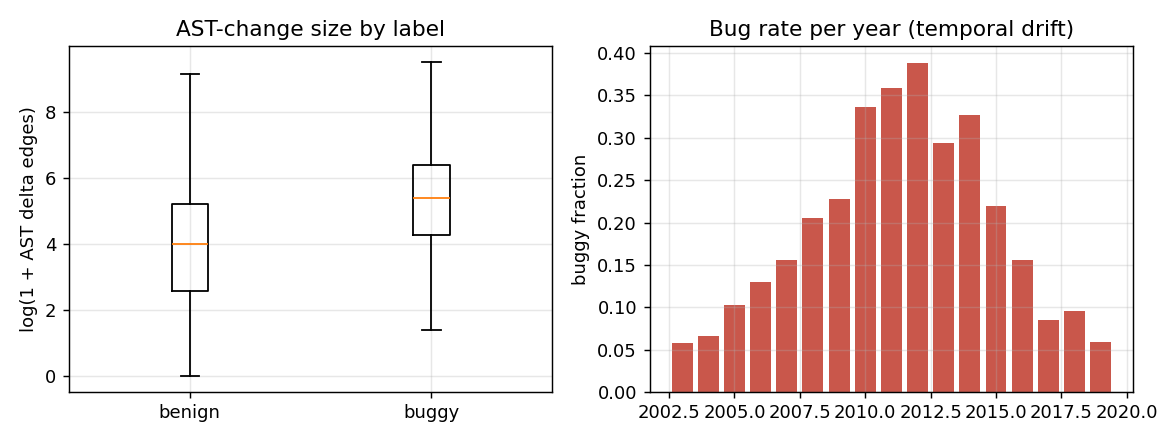
\includegraphics[width=.92\linewidth]{bug_signal.png}
		\caption{Left: AST-change size (log delta edges) for benign vs.\ buggy commits.
			Right: yearly bug rate, showing pronounced concept drift.}\label{fig:signal}
	\end{figure}

	\paragraph{Why every online trajectory declines toward the final commits.}
	The per-year bug rate (\code{scalability/collect\_growth\_stats.py}, computed
	directly from the labelled commits) rises from $5.8\%$ (2003) to a peak of
	$39.0\%$ (2012), then falls steadily back to $9.5\%$ (2018) and $5.8\%$ (2019)
	--- essentially the 2003 level. This single fact, not a failure of any method,
	is what drags down \emph{every} rolling-window metric at the right edge of
	every trajectory figure in this document (Figures~\ref{fig:curves},
	\ref{fig:v1v2v3}, \ref{fig:v3traj}, \ref{fig:v4-final-streams} and their
	analogues): (i)~PR-AUC's achievable ceiling is bounded by the positive rate, so
	as positives thin out even a perfect model's PR-AUC shrinks; (ii)~a
	\code{ROLL}$=800$-commit rolling window at a $6\%$ rate contains only
	$\approx$$48$ positives versus $\approx$$310$ at the 2012 peak, so
	precision/recall/F1/MCC become noisier and, since the model's expanding-window
	training still carries substantial mass from the high-bug-rate middle years,
	systematically \emph{over-predict} ``buggy'' in this low-defect tail (the same
	miscalibration documented for the controlled $2018$--$2019$ split,
	\S\ref{sec:closeout}, \S\ref{sec:roadmapB}); (iii)~ROC-AUC is comparatively more
	robust to the rate itself but still dips because the relational/structural
	priors are seeded from the same rare, less-informative recent positives. This
	is a real property of the Groovy history, not an artefact of one model: every
	baseline and every KG variant declines together into the tail
	(Figure~\ref{fig:v1v2v3}), which is precisely why the fully-online prequential
	protocol --- rather than a single static split --- is used throughout: it is
	designed to \emph{expose} concept drift rather than hide it, and the
	meaningful comparison in that regime is \emph{relative} (which curve declines
	least / stays on top), not the absolute end-of-stream value.

	% ===========================================================================
	\section{Audit and Data Quality of the Finalized KG}\label{sec:audit}
	% ===========================================================================
	We audited the complete graph (see \texttt{neo4j\_queries.txt}, Section~13). The
	schema is clean and coverage is high; the few gaps are small and explainable.
	
	\begin{center}
		\begin{tabular}{@{}p{9.2cm}rl@{}}
			\toprule
			\textbf{Check} & \textbf{Result} & \textbf{Verdict}\\
			\midrule
			in\_jit commits carrying an AST delta & 7{,}521 / 8{,}059 & expected\\
			in\_jit commits with \emph{no} AST delta & 538 & explainable$^{a}$\\
			\texttt{.java} files modified by a labelled commit but never parsed & 5 & gap$^{b}$\\
			Files with $>$1 AST root (duplicate-attach bug) & 0 & clean\\
			No-op \edge{UPDATES} (\code{old\_value}=\code{new\_value}) & 4 & negligible\\
			Removed nodes lacking a \edge{REMOVES} edge & 0 & clean\\
			\node{File} nodes total & 5{,}655 & ---\\
			\quad \texttt{.java} with an AST & 3{,}006 & expected\\
			\quad \texttt{.java} \emph{without} an AST & 2{,}628 & out-of-scope$^{c}$\\
			\quad non-\texttt{.java} (\texttt{.groovy}, \texttt{temp/}) & 21 & expected\\
			\bottomrule
		\end{tabular}
	\end{center}
	
	\footnotesize
	$^{a}$ These commits changed only non-Java files (build scripts, resources,
	docs) or made import-only/whitespace edits that produce no AST-structural change.
	$^{b}$ Six Java files fail both the JavaParser and JDT parsers (unusual legacy
	syntax in the old \texttt{lexer/}/\texttt{parser/} sources); they have
	commit/file nodes but no AST subtree. $^{c}$ \textbf{Important scoping fact:}
	\node{File} nodes are created from the \emph{full} ingested commit history, but
	the AST/delta layer is grown only for files touched by the 8{,}059 labelled
	(\code{in\_jit}) commits. Of the 2{,}628 \texttt{.java} files without an AST,
	only \textbf{6} were ever touched by a labelled commit (the parser-failure gaps
	above); the other $\approx$2{,}622 were touched \emph{only by non-labelled
		commits} and are therefore intentionally outside the modelled scope. This does
	not affect inference, which uses only the labelled commits and their deltas.
	\normalsize
	
	% ===========================================================================
	\section{Strengths and Limitations for Commit-Level Bug Detection}\label{sec:limits}
	% ===========================================================================
	\subsection*{Strengths}
	\begin{itemize}[nosep]
		\item \textbf{Change in context.} A commit is linked to the \emph{exact} AST
		nodes it touched \emph{and} to the surrounding code structure, so a GNN
		can reason over both the change and its neighbourhood --- richer than
		hand-crafted JIT metrics alone.
		\item \textbf{Lossless, incremental history.} Every file's evolution is
		captured exactly (recall 1.0) with only deltas stored; removed nodes are
		retained, so any past state is reconstructable.
		\item \textbf{Multi-modal.} Process signals (author, churn, issue links,
		history spine) and code-structure signals live in one graph and can be
		combined.
		\item \textbf{Online-ready.} Chronological \code{author\_ts} ordering and the
		arrival model directly support time-aware train/test splits and
		streaming evaluation, avoiding look-ahead leakage.
		\item \textbf{Labels built in.} ApacheJIT buggy/benign plus JIT metrics are on
		every commit node.
	\end{itemize}
	
	\subsection*{Limitations}
	\begin{itemize}[nosep]
		\item \textbf{Filtered commit set.} Only the 8{,}059 ApacheJIT commits are
		grown; deltas between two consecutive labelled commits that touch the
		same file therefore bundle any intervening \emph{unlabelled} commits.
		The change attributed to a commit is ``since the last labelled touch,''
		which may slightly differ from its raw git parent diff.
		\item \textbf{Java-only.} Non-\texttt{.java} files (build scripts, resources)
		are not modelled at the AST level.
		\item \textbf{File renames are modelled as add-of-new-path.} The delta engine
		(\texttt{build\_online\_kg.py}) treats a git rename (\code{R}) as an
		\code{ADD} of the new path: the new file is parsed afresh and every node is
		attributed to the commit via \edge{ADDS}, and the \emph{old} path's AST is
		not marked \code{alive=false}. So a rename inflates the commit's \edge{ADDS}
		count and leaves the pre-rename subtree as an alive ``ghost.'' The
		process-layer \edge{RENAMED\_FROM}/\edge{RENAMED\_TO} edges still record the
		rename, but the AST/delta layer does not thread node identity across a rename.
		This is \emph{not} rare: the history contains \textbf{2{,}289} \texttt{.java}
		renames, and \textbf{1{,}850} rename-source files still carry an alive AST
		(``ghost'' subtrees) in the current graph. The effect is (a) inflated
		\edge{ADDS}-size features on rename commits and (b) ghost files that no longer
		exist at \texttt{HEAD} but remain alive. The engine is patched to retire the
		old path going forward; the \emph{current} graph is documented-as-is for V2
		and a rename-aware replay is a V3 item (\S\ref{sec:v2finalize},
		Table~\ref{tab:v2finalize}).
		\item \textbf{\edge{AST\_CHILD} is not re-wired on \edge{MOVES}/re-insert.} A
		node that is moved or re-inserted keeps its old parent edge and may gain a new
		one, so $\approx$\,20k nodes ($<0.6\%$) have more than one incoming
		\edge{AST\_CHILD}; the live tree is therefore a near-tree (a DAG in those
		spots). The \emph{alive}-position invariant still holds; only the parent
		multiplicity is affected.
		\item \textbf{Coarse value handling.} \edge{UPDATES} captures a node's value
		change but not deep semantic equivalence; renames look like updates.
		\item \textbf{Identifier leaves lack positions} and are matched structurally
		only; very large refactors can stress the heuristic matcher (still
		consistent, but matches may be sub-optimal versus a full GumTree).
		\item \textbf{Label semantics.} ApacheJIT labels are derived (SZZ-style); they
		carry the usual noise of automatically mined defect labels.
		\item \textbf{Operational.} The build is long (hours) and, in this version,
		used a large resumable checkpoint; node identity should move onto the
		graph to keep checkpoints small (see next steps).
	\end{itemize}
	
	% ===========================================================================
	\section{Downstream Inference}\label{sec:inference}
	% ===========================================================================
	This section reports the first inference suite built on top of the KG. Because
	the target hardware has \emph{no GPU}, every method is deliberately light and
	\textbf{GNN-free}; the goal is both a usable defect predictor and a set of strong
	baselines a future GNN must beat. All code lives in \texttt{inference/}.
	
	\subsection{Problem framing (theory)}
	Just-in-time (JIT) defect prediction is a \emph{streaming binary
		classification} problem: each commit $C$ is a point with label
	$y_C\in\{\text{buggy},\text{benign}\}$, and predictions must be made
	\emph{at commit time} using only information available then. Formally, for a
	commit arriving at time $t_C$ (\code{author\_ts}), a model may use any data from
	commits with $t<t_C$ but nothing from the future. This rules out a random
	train/test split (which leaks future information) and demands a
	\emph{prequential} (predict-then-update) protocol. The positive class is rare
	($\approx$20\%), so threshold-free ranking metrics --- ROC-AUC and especially
	PR-AUC (area under precision--recall) --- are the primary measures; F1/MCC at a
	$0.5$ threshold are secondary.
	
	\subsection{Features from the KG (theory + implementation)}
	Three feature families are read out of the graph
	(\texttt{extract\_features.py}, \texttt{run\_all.py}):
	\begin{description}[nosep,leftmargin=1.4em]
		\item[Process metrics.] The 12 ApacheJIT change metrics already on each
		\node{Commit} (size \code{la}/\code{ld}, dispersion \code{nf}/\code{ent},
		history/experience \code{age}/\code{ndev}/\code{aexp}\ldots). \emph{Theory:}
		larger, more scattered, less-familiar changes are historically more
		defect-prone. \emph{Practice:} read directly as a $12$-dim vector.
		\item[Delta-graph features.] Per commit, counts and node-type/group histogram
		of its \edge{ADDS}/\edge{REMOVES}/\edge{UPDATES}/\edge{MOVES} edges, plus
		``AST-change tokens'' \code{\{edge\}:\{ast\_type\}}
		(e.g.\ \code{ADDS:MethodInvocation}). \emph{Theory:} the \emph{shape} of a
		structural change carries risk information beyond its size. \emph{Practice:}
		one Cypher aggregation over the delta layer.
		\item[Topology.] The heterogeneous neighbourhood of a commit (its files,
		developer, issues, changed AST types) used by the propagation and
		embedding methods below.
	\end{description}
	
	\subsection{Methods (theory + implementation)}
	\begin{description}[nosep,leftmargin=1.4em]
		\item[JIT-metrics baseline.] Logistic regression / random forest / gradient
		boosting on the 12 metrics --- the standard JIT predictor
		(\texttt{train\_eval.py}).
		\item[wvRN / relational priors.] \emph{Weighted-vote relational neighbour}: a
		commit's score is the historical bug-rate of the files and developer it
		touches, computed from the past only (\texttt{online\_infer.py}). Classic
		collective-classification baseline; very cheap, leakage-free.
		\item[Structural TF-IDF.] Treat each commit as a ``document'' of its AST-change
		tokens; TF-IDF $+$ linear model (\texttt{advanced\_infer.py}). Learns
		\emph{which kinds} of edits predict bugs.
		\item[Personalized PageRank (PPR).] Random-walk-with-restart label propagation
		over the heterogeneous KG, seeded from past buggy vs.\ benign commits;
		a commit is scored by relative proximity to each class
		(\texttt{advanced\_infer.py}). The textbook non-GNN graph inference.
		\item[KG embeddings.] Shallow, CPU-only graph embeddings feeding a linear
		classifier (\texttt{kge\_infer.py}): \emph{Truncated-SVD/LSA} of the
		commit--hub matrix; \emph{node2vec/DeepWalk} random-walk skip-gram
		(gensim); and \emph{TransE}/\emph{DistMult} knowledge-graph embeddings
		(PyKEEN, trained without the costly link-prediction evaluation).
		\item[Fusion.] Early fusion (one regularised linear model) over JIT metrics
		$+$ structural TF-IDF $+$ relational priors $+$ PPR score
		(\texttt{run\_all.py}).
	\end{description}
	
	\subsection{Evaluation protocols}
	Two protocols are run for every method. \textbf{Offline} uses a single
	time-ordered $70/30$ split (train on the older $70\%$). \textbf{Online}
	(prequential) warms up on the first $40\%$ then streams the rest in blocks,
	predicting each block from a model trained only on strictly earlier commits
	(expanding window). Online is the protocol that matches deployment; offline is a
	convenient sanity check. Leakage controls: scalers/vectorisers/embedding
	classifiers are fit on past data only, and the PPR score is computed with
	chronological folds so a commit is never among its own seeds.
	
	\subsection{Results}
	Tables~\ref{tab:off} and~\ref{tab:on} give every method in both protocols
	(consolidated by \texttt{run\_all.py}; the executed notebook
	\texttt{experiments/notebooks/inference\_results.ipynb} renders the same numbers
	as bar charts, ROC/PR curves and a heatmap). Random PR-AUC equals the positive
	rate: $0.163$ offline, $0.245$ online.
	
	\begin{table}[h]\centering\small
		\caption{Offline (time-ordered $70/30$ split).}\label{tab:off}
		\begin{tabular}{@{}lrrrr@{}}
			\toprule
			\textbf{Method} & \textbf{ROC-AUC} & \textbf{PR-AUC} & \textbf{F1} & \textbf{MCC}\\
			\midrule
			JIT-metrics (baseline) & 0.739 & 0.355 & 0.411 & 0.280\\
			wvRN / priors          & 0.787 & 0.408 & 0.081 & 0.127\\
			Structural TF-IDF      & 0.731 & 0.404 & 0.395 & 0.256\\
			PPR propagation        & 0.687 & 0.273 & 0.338 & 0.170\\
			KGE Truncated-SVD      & 0.691 & 0.306 & 0.382 & 0.234\\
			node2vec               & 0.749 & 0.405 & 0.399 & 0.264\\
			TransE                 & 0.726 & 0.360 & 0.386 & 0.247\\
			DistMult               & 0.768 & 0.438 & 0.437 & 0.317\\
			\textbf{Fusion}        & \textbf{0.820} & \textbf{0.542} & \textbf{0.477} & \textbf{0.376}\\
			\bottomrule
		\end{tabular}
	\end{table}
	
	\begin{table}[h]\centering\small
		\caption{Online (prequential, expanding window) --- the deployment protocol.}\label{tab:on}
		\begin{tabular}{@{}lrrrr@{}}
			\toprule
			\textbf{Method} & \textbf{ROC-AUC} & \textbf{PR-AUC} & \textbf{F1} & \textbf{MCC}\\
			\midrule
			JIT-metrics (baseline) & 0.679 & 0.398 & 0.453 & 0.218\\
			wvRN / priors          & 0.733 & 0.460 & 0.067 & 0.115\\
			Structural TF-IDF      & 0.750 & 0.489 & 0.519 & 0.333\\
			PPR propagation        & 0.681 & 0.351 & 0.471 & 0.245\\
			KGE Truncated-SVD      & 0.703 & 0.442 & 0.460 & 0.279\\
			node2vec               & 0.740 & 0.471 & 0.506 & 0.306\\
			TransE                 & 0.730 & 0.469 & 0.497 & 0.292\\
			DistMult               & 0.757 & 0.487 & 0.529 & 0.343\\
			\textbf{Fusion}        & \textbf{0.827} & \textbf{0.616} & \textbf{0.555} & \textbf{0.397}\\
			\bottomrule
		\end{tabular}
	\end{table}
	
	\begin{figure}[H]\centering
		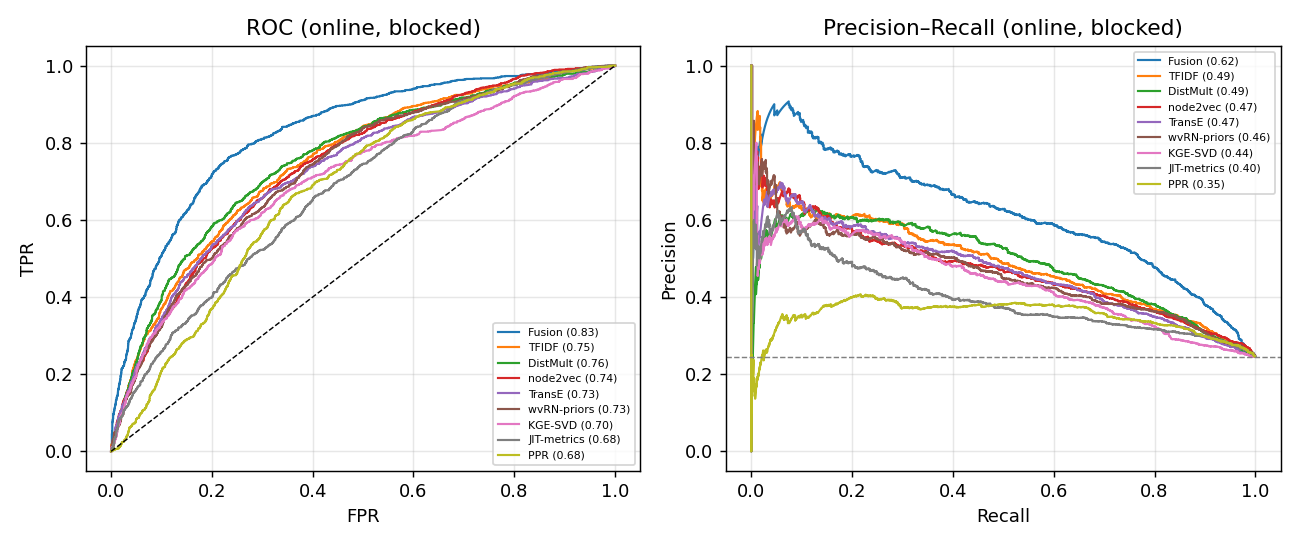
\includegraphics[width=\linewidth]{online_curves.png}
		\caption{Online (blocked) ROC and precision--recall curves. Fusion (top legend
			entry) dominates across the whole operating range; every KG-native method sits
			above the JIT-metrics baseline on PR.}\label{fig:curves}
	\end{figure}
	
	\subsection{Interpretation}
	\begin{itemize}[nosep]
		\item \textbf{Fusion is best by a wide margin}, and the gap is largest in the
		deployment-realistic online setting: PR-AUC $0.398\!\rightarrow\!0.616$
		over the JIT baseline ($+55\%$ relative), ROC $0.679\!\rightarrow\!0.827$,
		MCC $0.218\!\rightarrow\!0.397$. \emph{The KG's AST/delta and relational
			signals add real, complementary predictive value} on top of the classic
		metrics --- the central justification for the graph.
		\item \textbf{Every KG-native signal beats the metrics baseline on PR-AUC
			online.} The strongest \emph{single} signals are structural TF-IDF
		($0.489$) and the DistMult embedding ($0.487$): \emph{what kind} of AST
		change a commit makes, and \emph{where} the commit sits in the
		heterogeneous graph, are both individually informative.
		\item \textbf{Embeddings.} DistMult (bilinear) $>$ node2vec $\approx$ TransE
		$>$ Truncated-SVD, consistent with bilinear scoring capturing the
		commit--type--file relations better than a purely translational or
		linear-spectral model.
		\item \textbf{PPR alone is weak} ($0.351$): file/developer hubs connect buggy
		and benign commits indiscriminately, so raw proximity is noisy --- yet it
		still helps inside the fusion as one signal among many.
		\item \textbf{Online $>$ offline} for most methods because the
		expanding-window retraining \emph{adapts to concept drift} (the bug rate
		rises then falls across 2003--2019); this is exactly why the online
		protocol matters for JIT.
		\item \textbf{Caveat.} wvRN's near-zero F1 reflects an uncalibrated raw-rate
		score (its ranking, ROC/PR, is strong); a threshold/calibration step
		fixes the hard-decision metric.
	\end{itemize}
	
	\subsection{Controlled comparison to the project baselines}\label{sec:cmp}
	The within-project baselines in \texttt{baselines/} (notebook
	\texttt{WithinProj\_baselines.ipynb}) evaluate on a single \emph{chronological}
	split per project --- sort by \code{author\_date}, train on the first $70\%$,
	test on the \emph{last} $15\%$ (the middle $15\%$ validation block is unused) ---
	and report ROC-AUC and buggy-class F1. To compare fairly we re-ran our own
	features through that \emph{exact} split and test set
	(\texttt{inference/compare\_baselines.py}); every ``Ours'' row uses a
	\emph{balanced logistic regression}, identical to the baseline classifier, so any
	difference comes from the \emph{features}, not the learner. As a sanity check our
	JIT-metrics model reproduces the baseline logistic regression \emph{exactly}
	(ROC $0.698$, F1 $0.232$), confirming the protocols are aligned.
	
	\paragraph{Caution on the window.} This split's test set is the last $15\%$ of
	the timeline (2018--2019), where the bug rate is only $\approx$7.5\% --- a much
	lower and harder regime than the windows of
	Tables~\ref{tab:off}--\ref{tab:on} (bug rate $0.16$/$0.25$). Absolute scores are
	therefore lower here and are \emph{not} directly comparable to those tables;
	within Table~\ref{tab:base} everything is on the same footing.
	
	\begin{table}[h]\centering\small
		\caption{Controlled comparison on the baselines' chronological split (train first
			$70\%$, test last $15\%$; test bug rate $\approx0.075$). ``Ours'' rows use a
			balanced logistic regression on the named KG features.}\label{tab:base}
		\begin{tabular}{@{}lrr@{}}
			\toprule
			\textbf{Method} & \textbf{ROC-AUC} & \textbf{F1}\\
			\midrule
			\multicolumn{3}{@{}l}{\textit{Published baselines (\texttt{baselines/results})}}\\
			Naive: random / all-buggy & 0.500 & 0.09\,/\,0.13\\
			JIT metrics --- Logistic Regression & 0.698 & 0.232\\
			JIT metrics --- Random Forest (tuned) & 0.729 & 0.336\\
			JIT metrics --- XGBoost (tuned) & 0.755 & 0.267\\
			Text TF-IDF-768D --- Random Forest & \textbf{0.813} & 0.321\\
			\midrule
			\multicolumn{3}{@{}l}{\textit{Ours --- same split, balanced LR on KG features}}\\
			JIT-metrics (reproduces baseline LR) & 0.698 & 0.232\\
			Structural TF-IDF (AST tokens) & 0.637 & 0.217\\
			PPR propagation & 0.667 & 0.166\\
			KG embeddings (SVD / node2vec / TransE / DistMult) & 0.61--0.62 & $\sim$0.21\\
			wvRN / relational priors & 0.743 & 0.000\\
			\textbf{Fusion (JIT $+$ TF-IDF $+$ priors $+$ PPR)} & \textbf{0.732} & \textbf{0.236}\\
			\bottomrule
		\end{tabular}
	\end{table}
	
	\paragraph{Honest reading.}
	\begin{itemize}[nosep]
		\item Our \textbf{Fusion (ROC $0.732$)} is \emph{competitive with the tuned
			traditional-metric baselines} (RF-tuned $0.729$, just under
		XGBoost-tuned $0.755$) and well above plain JIT-LR ($0.698$), but it does
		\textbf{not} beat the strongest baseline --- a \emph{text} TF-IDF-768D
		model ($0.813$).
		\item Our individual KG-native methods \emph{underperform} on this hard,
		low-bug tail window (ROC $0.61$--$0.74$) --- noticeably weaker than they
		look on the easier windows of Tables~\ref{tab:off}--\ref{tab:on}.
		\item The decisive gap is that the best baseline uses \textbf{commit-message /
			code text} (a $768$-dim embedding), a signal our KG inference does
		\emph{not} use at all. Code-structure and process signals alone are
		competitive with traditional metrics but not with strong text features on
		this split.
	\end{itemize}
	This \emph{corrects} an earlier, non-controlled comparison (which compared
	different test windows and overstated our advantage). The implication is the
	V3 critical path of \S\ref{sec:roadmapB}: lift commit text into a graph layer
	(\S\ref{sec:textlayer}) and move to a GNN that exploits the AST neighbourhood the
	tabular methods flatten away.
	
	\subsection{Fully-online (prequential) evaluation and operating-point F1}\label{sec:onlinejit}
	The strictest realisation of the JIT protocol processes commits \emph{one at a
		time}: as each commit arrives we (1)~\textbf{predict} it from the KG/history
	known so far, (2)~\textbf{evaluate} by revealing its label and updating running
	metrics, (3)~\textbf{grow} the KG state (its relational/graph evidence is added),
	and (4)~\textbf{learn} (incremental \code{partial\_fit} for linear models,
	periodic expanding-window retraining for trees/embeddings). The engine
	(\texttt{inference/online\_jit.py}) runs the within-project baselines \emph{and}
	the KG-native methods in this same stream, so they are compared under one
	identical online protocol (notebook
	\texttt{experiments/notebooks/online\_jit\_evaluation.ipynb}).
	
	\paragraph{Operating-point F1.} Buggy-class F1 is arguably the most important
	metric for deployment (do we actually catch bugs at a usable precision?), but F1
	at a fixed $0.5$ threshold is unfair to uncalibrated scores. We therefore report
	\code{F1\_online}: the buggy-F1 with the decision threshold \emph{tuned online}
	on past predictions only (re-tuned every $150$ commits). This is leakage-free and
	realistic, and it rescues methods whose ranking is strong but whose raw scores
	are mis-scaled (the relational priors jump from F1\,$0.05$ at $0.5$ to
	\code{F1\_online}\,$0.48$).
	
	\begin{table}[H]\centering\small
		\caption{Fully-online prequential results (whole stream; warm-up $30\%$, scored
			$\approx$5{,}640 commits, stream bug rate $0.245$). Sorted by online
			operating-point F1.}\label{tab:jit}
		\begin{tabular}{@{}lrrrr@{}}
			\toprule
			\textbf{Method} & \textbf{F1\_online} & \textbf{F1@.5} & \textbf{PR-AUC} & \textbf{ROC}\\
			\midrule
			\multicolumn{5}{@{}l}{\textit{Within-project baselines}}\\
			LR / JIT metrics            & 0.464 & 0.467 & 0.348 & 0.671\\
			RandomForest / JIT metrics  & 0.478 & 0.240 & 0.478 & 0.723\\
			GradBoost / JIT metrics     & 0.481 & 0.445 & 0.469 & 0.711\\
			Naive prior bug-rate        & 0.391 & 0.000 & 0.223 & 0.468\\
			\midrule
			\multicolumn{5}{@{}l}{\textit{KG-native methods}}\\
			Relational priors (wvRN)    & 0.477 & 0.048 & 0.428 & 0.703\\
			Structural TF-IDF           & 0.490 & 0.486 & 0.420 & 0.719\\
			Personalized PageRank       & 0.511 & 0.512 & 0.383 & 0.727\\
			KG embedding (SVD/LSA)      & 0.479 & 0.460 & 0.427 & 0.690\\
			\textbf{Fusion (M+T+R+P)}   & \textbf{0.593} & \textbf{0.552} & \textbf{0.598} & \textbf{0.822}\\
			\bottomrule
		\end{tabular}
	\end{table}
	
	\begin{figure}[H]\centering
		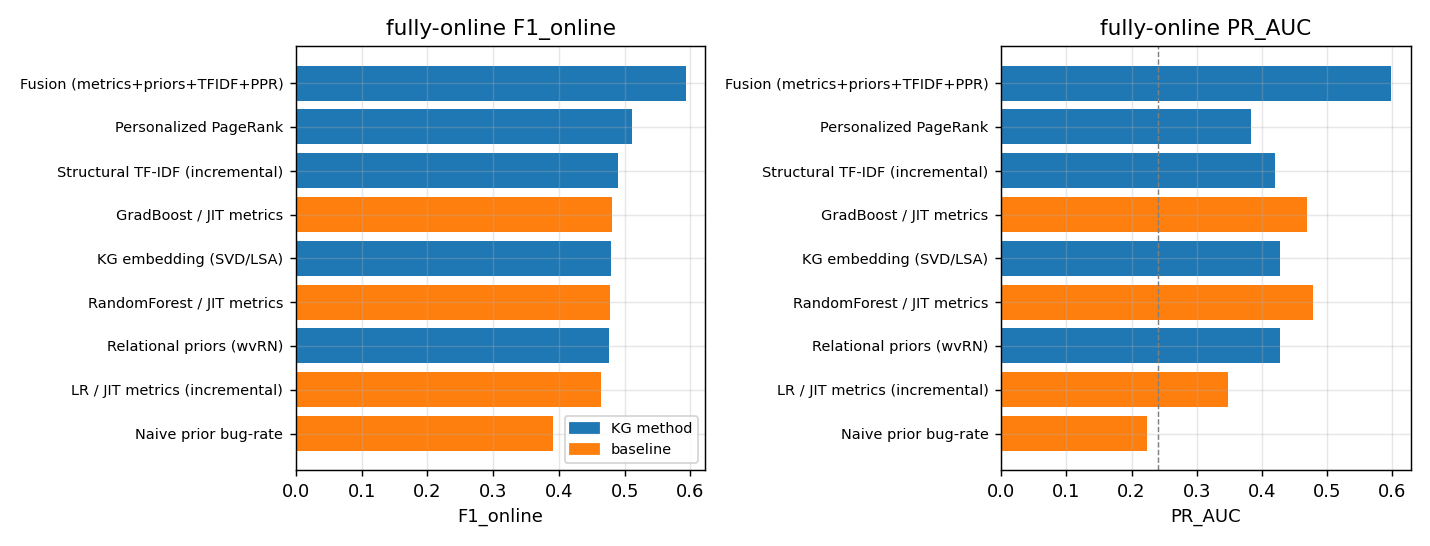
\includegraphics[width=\linewidth]{online_jit_compare.png}\\[3pt]
		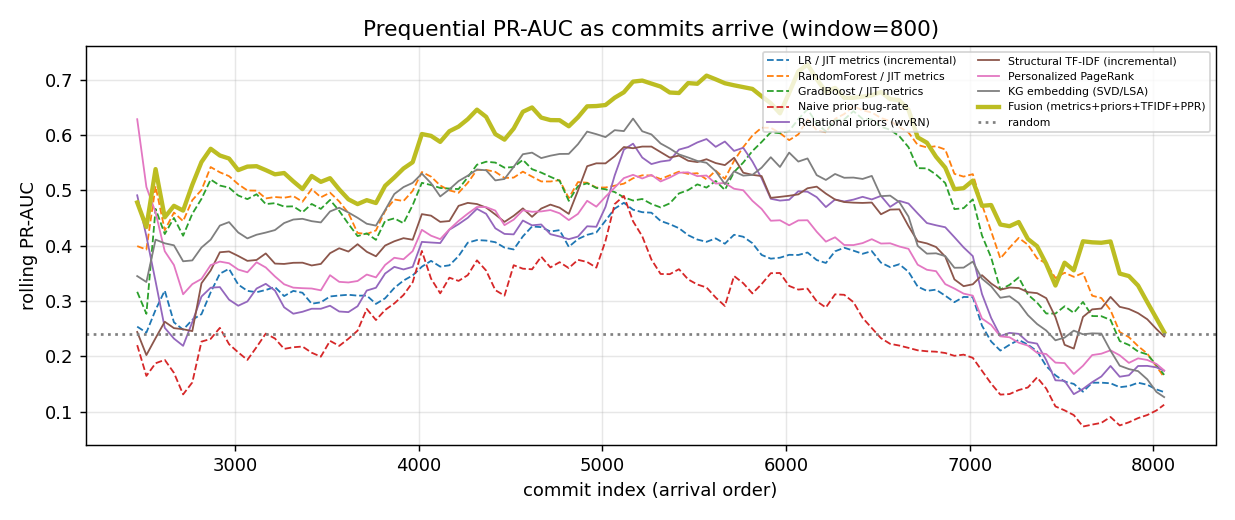
\includegraphics[width=.80\linewidth]{jit_trajectories.png}
		\caption{Top: fully-online operating-point F1 (\code{F1\_online}) and PR-AUC
			(baselines orange, KG-native blue). Bottom: rolling PR-AUC \emph{as commits
				arrive} --- the Fusion (thick blue) stays on top throughout the stream.}\label{fig:jit}
	\end{figure}
	
	Under the strict per-commit protocol the \textbf{Fusion again leads on every
		metric, including the operating-point F1} (\code{F1\_online} $0.593$ vs.\ $0.481$
	for the best baseline), and the trajectory shows the lead is \emph{persistent}.
	
	\paragraph{Fusion feature ablation.} The Fusion combines four streams:
	\textbf{M} = JIT metrics, \textbf{T} = structural TF-IDF, \textbf{R} = relational
	priors, \textbf{P} = PPR score. We evaluate all $15$ non-empty subsets under the
	same online protocol (Figure~\ref{fig:abl}); the leave-one-out drop in
	\code{F1\_online} measures each feature's unique contribution.
	
	\begin{figure}[H]\centering
		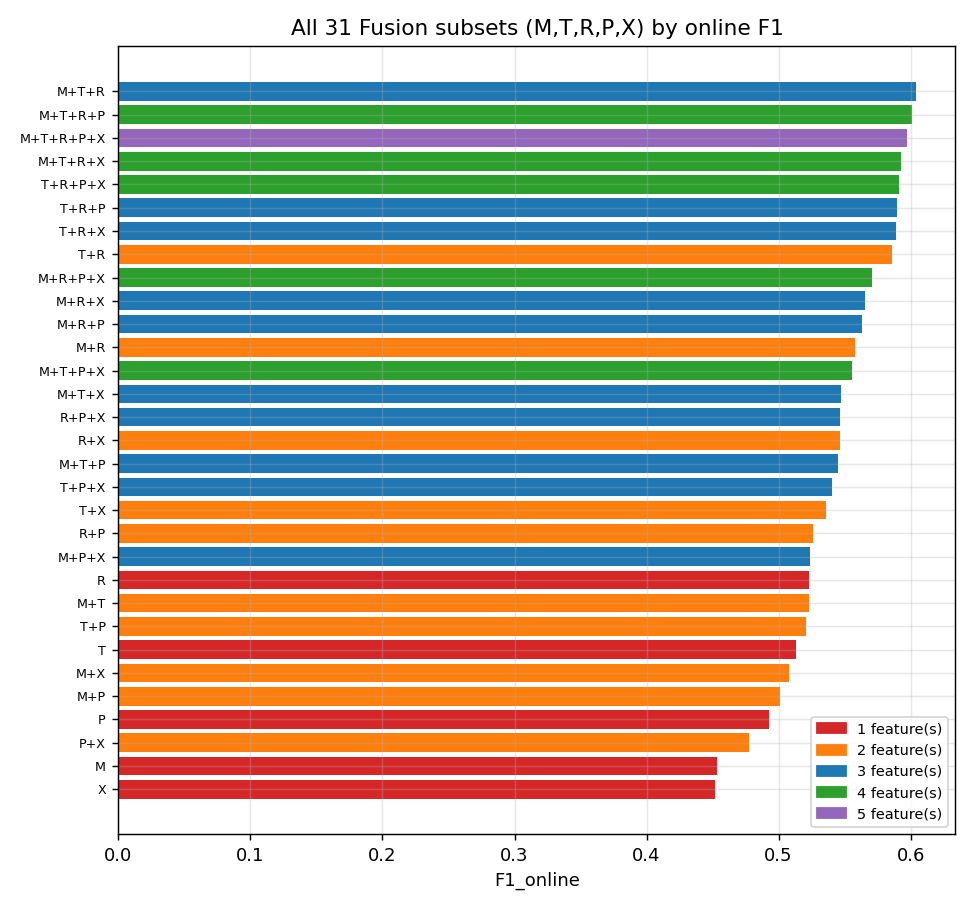
\includegraphics[width=.60\linewidth]{ablation_combos.png}\\[3pt]
		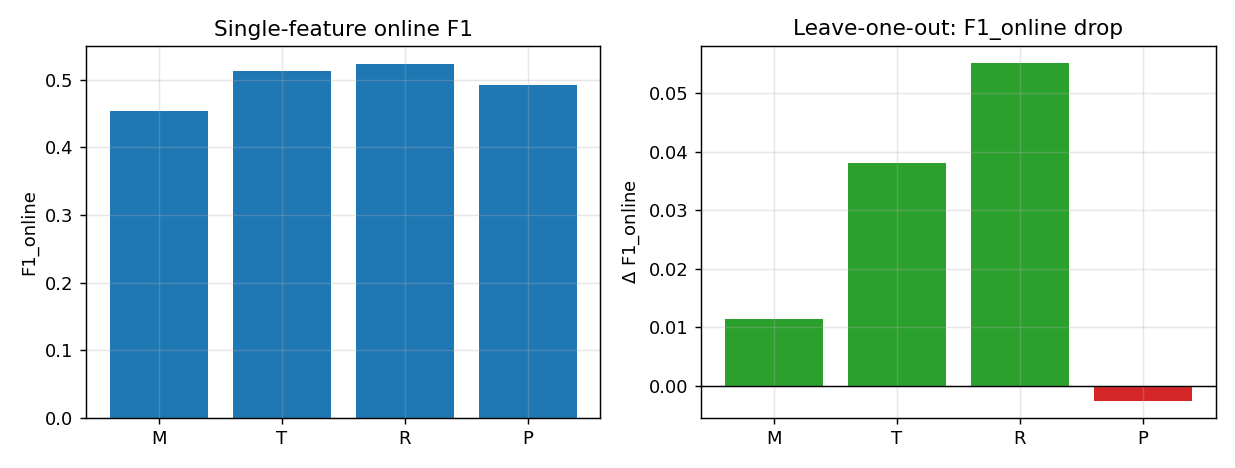
\includegraphics[width=.84\linewidth]{ablation_importance.png}
		\caption{Top: all $15$ feature subsets ranked by online F1 (colour $=$ number of
			features). Bottom-left: each feature alone. Bottom-right: leave-one-out drop in
			\code{F1\_online} when a feature is removed from M+T+R+P (negative $=$ the feature
			slightly hurts).}\label{fig:abl}
	\end{figure}
	
	Findings (consistent across \code{F1\_online} and PR-AUC):
	\begin{itemize}[nosep]
		\item \textbf{Relational priors (R) and structural TF-IDF (T) are the core.}
		They are the strongest single features (\code{F1\_online} $0.52$ / $0.51$)
		and have the largest leave-one-out drops ($-0.055$ and $-0.038$); together
		(T+R) they already reach \code{F1\_online} $0.587$.
		\item \textbf{JIT metrics (M) add a small positive boost}
		(T+R\,$\to$\,M+T+R: $0.587\!\rightarrow\!0.604$).
		\item \textbf{PPR (P) is redundant / marginally harmful}: removing it
		\emph{improves} the result (leave-one-out $+0.003$), so the best subset is
		\textbf{M+T+R} (\code{F1\_online} $0.604$, PR-AUC $0.608$), edging the full
		four-feature fusion --- its graph-proximity signal is already captured by
		the relational priors.
	\end{itemize}
	\textbf{Recommendation.} The Fusion's sweet spot is \textbf{M+T+R}; PPR can be
	dropped with no loss (a small gain) and lower cost.
	
	\paragraph{Reproducibility.} \texttt{python inference/run\_all.py} rebuilds all
	features, embeddings (cached under \texttt{outputs/emb\_*.npy}) and the results
	cache; the notebook then loads the cache (no Neo4j needed) and draws the
	comparison. Per-method entry points: \texttt{train\_eval.py} (tabular ablation),
	\texttt{advanced\_infer.py} (TF-IDF/PPR/fusion), \texttt{online\_infer.py}
	(prequential O1--O6), \texttt{kge\_infer.py} (node2vec/TransE/DistMult).
	
	% ===========================================================================
	\section{Version 2 --- Debugging and Refinement}\label{sec:v2}
	% ===========================================================================
	V2 refines the finalized KG \emph{in place} (no rebuild), with two workstreams:
	data-quality debugging and a commit-message text feature. A diagnostic audit
	(\texttt{v2\_audit.py}) is the before/after yardstick.
	
	\subsection{Data-quality debugging}
	Table~\ref{tab:v2audit} shows the audit before and after the fixes
	(\texttt{v2\_cleanup.py}, \texttt{recover\_unparseable.py},
	\texttt{recover\_treesitter.py}).
	
	\begin{table}[H]\centering\small
		\caption{V2 data-quality audit, before $\rightarrow$ after.}\label{tab:v2audit}
		\begin{tabular}{@{}lrrl@{}}
			\toprule
			\textbf{Issue} & \textbf{Before} & \textbf{After} & \textbf{Fix}\\
			\midrule
			\code{alive=NULL} base nodes        & 22{,}943 & 0 & normalised to \code{true}\\
			no-op \edge{UPDATES} (old$=$new)    & 4        & 0 & deleted\\
			legacy \node{ASTDiff}/\node{ASTEdit}& 10/491   & 0 & removed\\
			unparseable \texttt{.java} gap files& 6        & \textbf{0} & all recovered (1 javalang $+$ 5 tree-sitter)\\
			\bottomrule
		\end{tabular}
	\end{table}
	
	Two findings stand out. (i) The \textbf{532 ``suspect-skip'' commits}
	(\textbf{745} (commit,file) pairs that modified an AST-bearing file yet carry no
	delta) were diagnosed (\texttt{recover\_skipped\_deltas.py}). They split into a
	cleanly-separable \emph{safe} subset --- \textbf{111} pairs where the commit is
	the \emph{last} labelled toucher of the file, so the graph's stored state is
	exactly that commit's ``before'' and the diff can be checked directly --- and a
	\textbf{634}-pair \emph{bundled} residual (a later labelled commit also touches
	the file). Re-diffing every safe pair finds \textbf{0 recoverable deltas}: 103
	are \emph{genuine no-ops} (whitespace/comment/import edits with no AST change)
	and 8 are git/parse gaps, so \emph{no real structural change was dropped for the
	verifiable subset}. The 634 bundled pairs are \emph{not} re-diffed here: their
	change is attributed to the next labelled commit that touches the file (the
	documented filtering behaviour of \S\ref{sec:online}), so per-commit they are
	delta-less \emph{by design} but the file-level change is preserved downstream.
	\emph{Honest caveat:} ``no data was lost'' is \textbf{verified} for the safe
	subset and \textbf{assumed} (not yet spot-checked) for the bundled residual;
	closing that is a finalization item (\S\ref{sec:v2finalize}). Note also that
	$\approx$96 of the 532 are commits touching the tree-sitter-recovered antlr4
	files, whose per-commit deltas are deliberately deferred (below).
	(ii) The remaining unparseable files are
	\emph{modern-Java} sources (the antlr4 \texttt{AstBuilder.java}, Java-8 functional
	interfaces) that the old \texttt{javalang} parser cannot handle. We close the gap
	with a \textbf{tree-sitter} Java parse path (\texttt{recover\_treesitter.py}):
	these files have no existing AST, so building them with a different but
	\emph{consistent} parser is conflict-free, and a snake\_case$\rightarrow$PascalCase
	type map keeps \code{ast\_type} uniform with the rest of the graph. All 5 are
	attached ($+$63{,}982 \node{ASTNode}s, all \texttt{.java} files now have an AST).
	Their \emph{per-commit delta} history is left unbuilt by default: the cross-parser
	subtree-hash diff on these very large, heavily-refactored files yields disproportion-
	ately large/noisy deltas ($\sim$$+$384k nodes, $\sim$$+$112k spurious \edge{MOVES})
	that would distort the graph, so delta replay is an opt-in flag deferred to a
	dedicated cross-parser-diff effort.
	
	\subsection{Commit-message text feature}
	Commit messages (present on 8{,}054/8{,}059 commits) are added as a fifth fusion
	stream \textbf{X} (a hashing TF-IDF of the message), evaluated under the same
	online protocol. The extended ablation now spans all $31$ subsets of
	$\{$M,T,R,P,X$\}$ (Figure~\ref{fig:v2abl}).
	
	\begin{figure}[H]\centering
		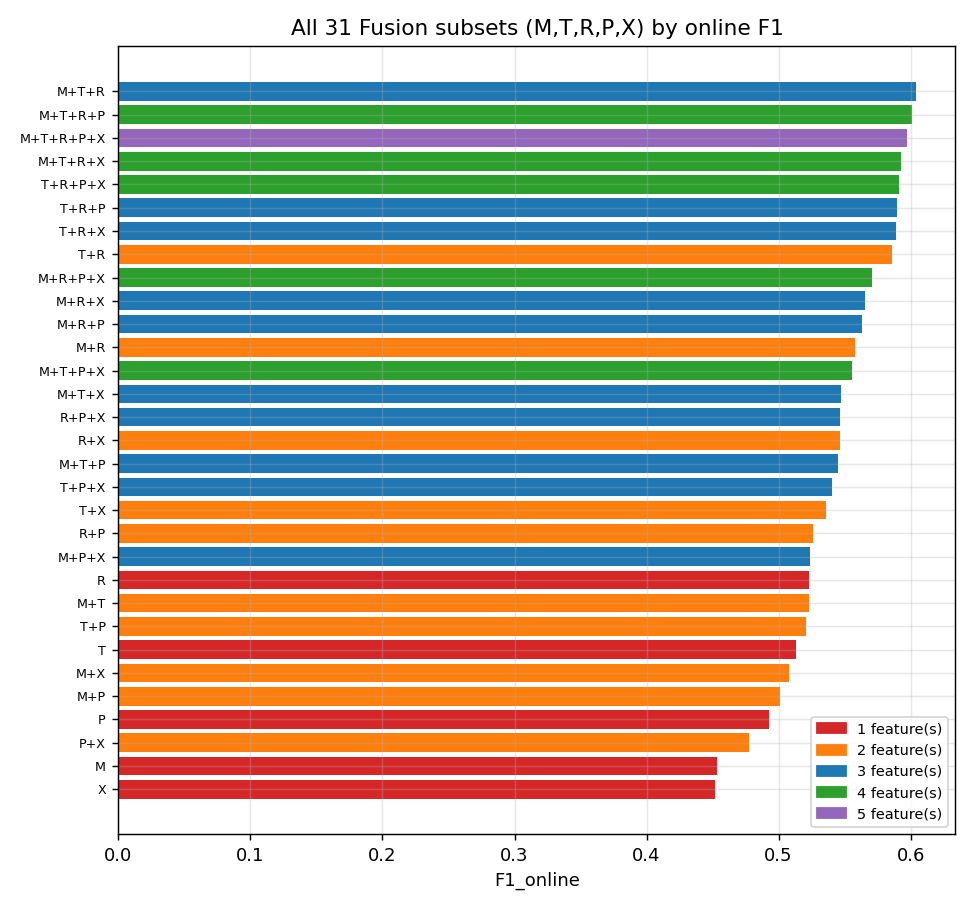
\includegraphics[width=.62\linewidth]{ablation_combos.png}
		\caption{All $31$ Fusion subsets ranked by online operating-point F1 (colour $=$
			number of features). Adding the commit-text stream \textbf{X} does not raise the
			top of the ranking: \textbf{M+T+R} (no text, no PPR) remains the best on online
			F1.}\label{fig:v2abl}
	\end{figure}
	
	The result is honest and instructive:
	\begin{itemize}[nosep]
		\item \textbf{In the online stream}, the message TF-IDF is the \emph{weakest}
		single feature (F1\_online $0.452$, PR-AUC $0.408$) and does \emph{not}
		improve the fusion --- \textbf{M+T+R} stays best on F1 ($0.604$); the full
		M+T+R+P+X only nudges PR/ROC ($0.610$/$0.830$) while lowering F1.
		\item \textbf{On the hard controlled split} (the low-defect tail where text
		mattered most), text \emph{does} help modestly: Fusion$+$text improves
		ROC $0.733\!\rightarrow\!0.740$ and F1 $0.236\!\rightarrow\!0.261$, and a
		text-only model reaches PR-AUC $0.254$ (best of our methods there).
		\item But a simple bag-of-words text still \textbf{does not close the gap} to
		the external $768$-dim \emph{transformer} text baseline (ROC $0.813$).
	\end{itemize}
	\textbf{Takeaway.} A cheap message TF-IDF gives a small, regime-dependent boost;
	genuinely beating the strong text baseline needs a real text encoder
	(CodeBERT-style message/diff embeddings) --- promoted to a V3 priority.

	\paragraph{Single features vs.\ the fusion, as commits arrive.} The $31$-subset
	bar chart (Figure~\ref{fig:v2abl}) ranks configurations by their
	\emph{whole-stream} score and hides \emph{when} each signal is informative.
	Figure~\ref{fig:v2traj} instead plots a \emph{rolling} PR-AUC (a sliding window
	of the last $800$ scored commits) for each of the five single streams
	--- \textbf{M}\,(JIT metrics), \textbf{T}\,(structural TF-IDF),
	\textbf{R}\,(relational priors), \textbf{P}\,(PPR), \textbf{X}\,(commit-text)
	--- against the full \textbf{M+T+R+P+X} fusion, along commit arrival order. It
	reads as a time series of how each signal performs through the 2003--2019
	stream, with the dotted line marking the random PR-AUC (the local positive
	rate $\approx0.245$).

	\begin{figure}[H]\centering
		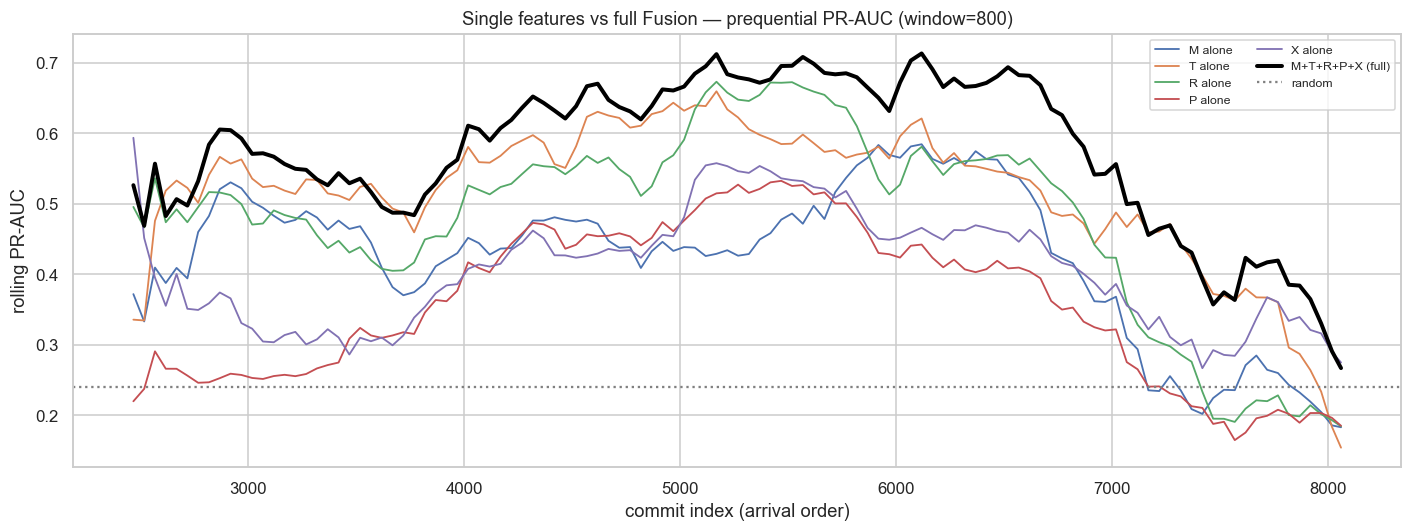
\includegraphics[width=\linewidth]{ablation_single_vs_fusion_traj.png}
		\caption{Rolling prequential PR-AUC (window $=800$ commits) of each single
			feature alone versus the full \textbf{M+T+R+P+X} fusion, as a function of
			commit arrival order. The fusion (thick black) sits \emph{above every single
				stream essentially throughout} the run, confirming the gain is persistent
			rather than an artefact of any one window. Among the singles, \textbf{T} and
			\textbf{R} (orange/green) are the consistent leaders, while \textbf{M},
			\textbf{P} and the commit-text \textbf{X} (blue/red/purple) trail; \textbf{X}
			is never the best single signal at any point in the stream --- the per-arrival
			view of why text does not lift the online fusion. All curves fall together into
			the low-defect $2018$--$2019$ tail (right edge, dropping toward the random
			line), the same hard regime quantified in \S\ref{sec:cmp}.}\label{fig:v2traj}
	\end{figure}

	\subsection{\texorpdfstring{Statistical comparison: V1 $\rightarrow$ V2}{Statistical comparison: V1 to V2}}\label{sec:v2stat}
	V2 changes the graph \emph{minimally and only where intended}: it cleans flag/
	legacy artefacts and recovers 6 previously-unparseable files (1 via javalang,
	5 via tree-sitter); the entire commit/AST/delta substance of V1 is preserved.
	The javalang recovery gave \textbf{2} more commits a delta (in\_jit-with-delta
	$7{,}521\!\rightarrow\!7{,}523$); the suspect-skip diagnosis confirmed no real
	structural change was dropped for the verifiable safe subset (the bundled
	residual is preserved downstream, \S\ref{sec:v2finalize}).
	Table~\ref{tab:v2stat} contrasts the key graph
	statistics; the large structural counts (\node{ASTNode}, \edge{AST\_CHILD},
	\edge{ADDS}/\edge{REMOVES}/\edge{MOVES}/\edge{UPDATES}, \node{Commit}, deltas per
	commit) are \emph{unchanged} apart from the $+19$ nodes / $+1$ file from the one
	recovered source.
	
	\begin{table}[H]\centering\small
		\caption{Graph statistics, V1 vs.\ V2 (only the deliberately-changed quantities
			differ).}\label{tab:v2stat}
		\begin{tabular}{@{}lrrl@{}}
			\toprule
			\textbf{Statistic} & \textbf{V1} & \textbf{V2} & \\
			\midrule
			\node{ASTNode} (total)              & 3{,}635{,}438 & 3{,}699{,}439 & $+63{,}982$ (6 recovered files)\\
			\node{File} with an AST             & 3{,}006       & 3{,}012       & $+6$ recovered\\
			\code{alive=true}                   & 2{,}805{,}375 & 2{,}892{,}319 & $+$ NULLs $+$ recovered nodes\\
			\code{alive=false} (history)        & 807{,}120     & 807{,}120     & unchanged\\
			\code{alive=NULL} (inconsistent)    & 22{,}943      & \textbf{0}    & normalised\\
			no-op \edge{UPDATES}                & 4             & \textbf{0}    & deleted\\
			legacy \node{ASTDiff}/\node{ASTEdit}& 10 / 491      & \textbf{0 / 0}& removed\\
			unparseable \texttt{.java} gap files& 6             & \textbf{0}    & all recovered (javalang $+$ tree-sitter)\\
			\midrule
			\multicolumn{4}{@{}l}{\textit{Unchanged between V1 and V2:}}\\
			\multicolumn{4}{@{}l}{\quad\edge{ADDS} 2{,}337{,}767 \;|\; \edge{REMOVES} 818{,}063 \;|\; \edge{MOVES} 147{,}330}\\
			\multicolumn{4}{@{}l}{\quad\node{Commit} 8{,}059 (in\_jit), 7{,}521 with deltas \;|\; \edge{AST\_CHILD} 3{,}652{,}425}\\
			\bottomrule
		\end{tabular}
	\end{table}
	
	\subsection{\texorpdfstring{Performance comparison: V1 $\rightarrow$ V2}{Performance comparison: V1 to V2}}\label{sec:v2perf}
	The only V2 change that can move the metrics is the new commit-text stream
	\textbf{X}; the data-quality fixes do not alter inference (they touch flags and a
	deprecated layer). We therefore compare the V1 fusion (M+T+R+P) against the V2
	variants under \emph{identical} protocols. Table~\ref{tab:v2perf} gives the
	fully-online prequential numbers (directly-comparable balanced-LR ablation) and
	the hard controlled-split numbers.
	
	\begin{table}[H]\centering\small
		\caption{Inference performance, V1 vs.\ V2. Top: fully-online prequential
			(operating-point F1 / PR-AUC / ROC). Bottom: controlled last-$15\%$ split
			(ROC / PR-AUC / F1).}\label{tab:v2perf}
		\begin{tabular}{@{}lrrr@{}}
			\toprule
			\multicolumn{4}{@{}l}{\textit{Fully-online prequential} \quad (F1\_online / PR-AUC / ROC)}\\
			\midrule
			\textbf{Fusion variant} & \textbf{F1\_online} & \textbf{PR-AUC} & \textbf{ROC}\\
			V1: M+T+R+P                         & 0.601 & 0.606 & 0.828\\
			V2: M+T+R+P+X \;(add text)          & 0.597 & \textbf{0.610} & \textbf{0.830}\\
			V2: M+T+R \;(recommended, drop PPR) & \textbf{0.604} & 0.608 & 0.828\\
			\midrule
			\multicolumn{4}{@{}l}{\textit{Controlled last-$15\%$ split} \quad (ROC / PR-AUC / F1)}\\
			\midrule
			\textbf{Fusion variant} & \textbf{ROC} & \textbf{PR-AUC} & \textbf{F1}\\
			V1: Fusion (no text)     & 0.733 & 0.204 & 0.236\\
			V2: Fusion $+$ text      & \textbf{0.740} & \textbf{0.217} & \textbf{0.261}\\
			\bottomrule
		\end{tabular}
	\end{table}
	
	\textbf{Reading the comparison.}
	\begin{itemize}[nosep]
		\item \textbf{Online (deployment) regime:} adding text is \emph{neutral} ---
		M+T+R+P+X nudges PR/ROC by $\le0.004$ while \emph{lowering} F1; the best
		configuration is V2's \textbf{M+T+R} (F1\_online $0.604$), which also drops
		PPR for lower cost. So V2's net online gain is essentially zero, but it
		\emph{simplifies} the recommended model.
		\item \textbf{Hard controlled regime:} text gives a \emph{small but real}
		improvement --- ROC $0.733\!\rightarrow\!0.740$, PR-AUC
		$0.204\!\rightarrow\!0.217$, F1 $0.236\!\rightarrow\!0.261$ --- consistent
		with text mattering more in the low-defect tail.
		\item \textbf{Overall:} V2 is best understood as a \emph{cleanup and honest
			negative/marginal result} on simple text, not a performance jump. The
		clear positive deltas are structural (zero inconsistencies, one recovered
		file) and methodological (the M+T+R recommendation); a substantial
		performance lift needs the richer text/encoder work deferred to V3.
	\end{itemize}

	\subsection{Baselines vs.\ KG-v1 vs.\ KG-v2 on online buggy-F1}\label{sec:v2base}
	The fully-online table of \S\ref{sec:onlinejit} (Table~\ref{tab:jit}) placed the
	within-project baselines next to the \emph{V1} KG-native methods; the V1$\to$V2
	comparison of \S\ref{sec:v2perf} (Table~\ref{tab:v2perf}) then compared the
	fusion \emph{variants} to each other. What was missing is a single picture that
	puts \emph{all three families on one axis} --- the baselines, the V1 inference
	methods, and the V2 (commit-text) methods --- under the one identical prequential
	protocol. Figure~\ref{fig:v2base} fills that gap on the deployment metric the
	project cares about most, the \textbf{online buggy-F1} (\code{F1\_online}), with
	PR-AUC alongside.

	\begin{figure}[H]\centering
		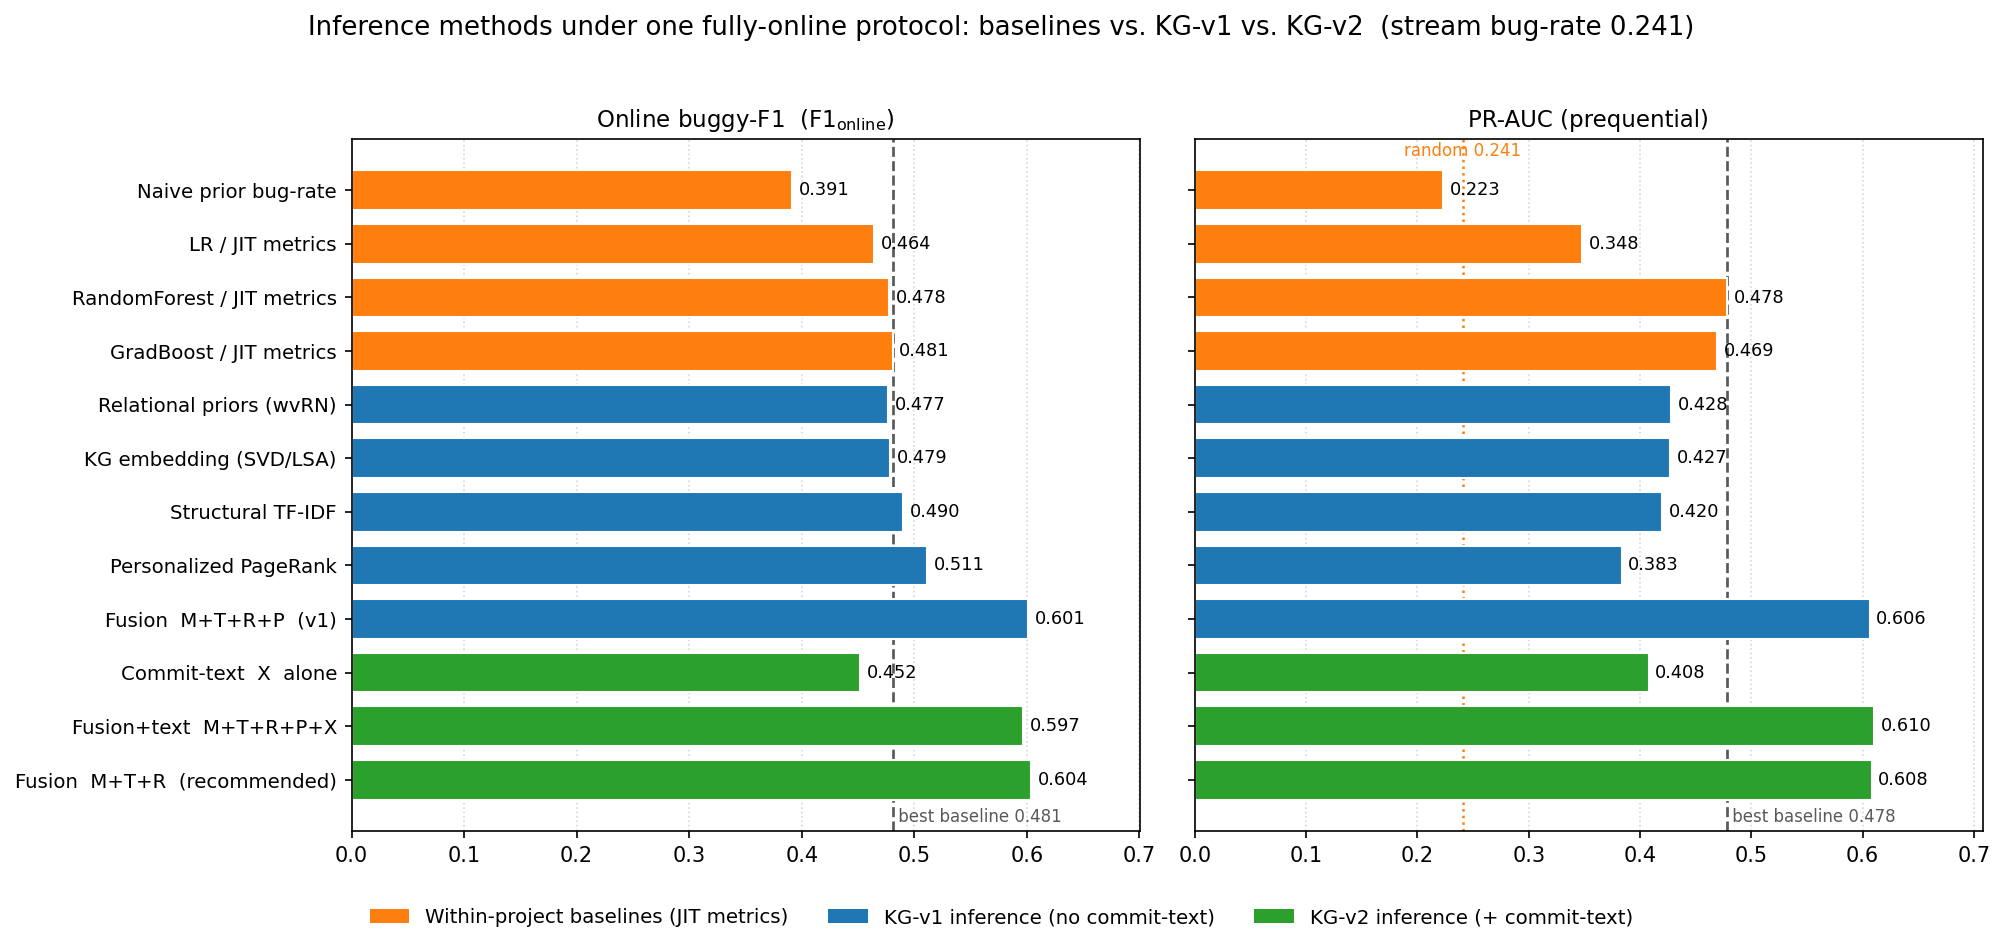
\includegraphics[width=\linewidth]{v1_v2_baseline_f1.png}
		\caption{All inference methods under the one fully-online (prequential)
			protocol, grouped by family: within-project \textbf{baselines}
			(\textcolor{kgorange}{orange}, JIT metrics only), \textbf{KG-v1} methods
			(\textcolor{kgblue}{blue}, no commit-text), and \textbf{KG-v2} methods
			(\textcolor{kggreen}{green}, $+$ commit-text stream \textbf{X}). Left:
			online buggy-F1 (\code{F1\_online}); right: prequential PR-AUC. The dashed
			line marks the strongest baseline (\code{F1\_online} $0.481$ / PR-AUC
			$0.478$, GradBoost on JIT metrics); the dotted orange line on the right is
			the random PR-AUC (stream bug-rate $0.241$). Single methods and baselines
			are from the streaming engine (\texttt{online\_jit.py}); the three Fusion
			bars are from the unified balanced-LR ablation
			(\texttt{online\_jit\_ablation\_v2.pkl}), so the V1 (M+T+R+P) vs.\ V2
			(M+T+R+P+X, M+T+R) deltas come from one engine and are directly comparable.
			Reproduce with \texttt{python docs/make\_v1\_v2\_baseline\_compare.py}.}
		\label{fig:v2base}
	\end{figure}

	The figure makes three things explicit at a glance:
	\begin{itemize}[nosep]
		\item \textbf{Every Fusion clears the best baseline.} All three fusion
		variants (V1 $0.601$, V2$+$text $0.597$, V2 M+T+R $0.604$) sit well to the
		right of the strongest baseline (GradBoost $0.481$) on \code{F1\_online}, and
		the gap is even larger on PR-AUC ($\sim$$0.61$ vs.\ $0.478$). The KG's
		structural/relational signal, not the learner, is what buys the lift --- the
		fusion uses the same balanced LR as the baseline.
		\item \textbf{KG-v2 is the best bar, but only marginally over KG-v1.}
		\textbf{M+T+R} (the recommended V2 model, PPR dropped) is the single best on
		\code{F1\_online} ($0.604$), edging the V1 four-feature fusion ($0.601$);
		adding the commit-text stream \textbf{X} on top (M+T+R+P+X) does \emph{not}
		help the online metric --- consistent with \S\ref{sec:v2perf}. V2's value here
		is a \emph{simpler, equally-strong} model, not a jump.
		\item \textbf{Commit-text alone is weak.} The \textbf{X}-only bar
		(\code{F1\_online} $0.452$, PR-AUC $0.408$) lands \emph{below} the JIT-metric
		baselines --- the per-method confirmation that a cheap bag-of-words message
		feature is the least informative single stream online, and why genuinely
		beating the strong external text baseline is deferred to a real encoder in V3.
	\end{itemize}

	\subsection{V2 finalization: known issues and their status}\label{sec:v2finalize}
	A pre-submission review of the build and inference code surfaced a small set of
	correctness/over-claim items; we record them here transparently with their
	resolution status, since a Q1 review is likely to probe exactly these points.

	\begin{table}[H]\centering\small
	\caption{V2 finalization checklist (status at submission).}\label{tab:v2finalize}
	\begin{tabular}{@{}p{6.4cm}p{2.2cm}p{6.0cm}@{}}
	\toprule
	\textbf{Issue} & \textbf{Severity} & \textbf{Status / resolution}\\
	\midrule
	Renames modelled as add-of-new-path; old AST not retired
	($2{,}289$ renames, $1{,}850$ ghost files) & medium--high (graph) &
	\textbf{Documented} as a limitation (\S\ref{sec:limits}); engine patched going
	forward; current graph not rebuilt --- rename-aware replay is a V3 item.\\
	\addlinespace
	Lossless-evolution claim was position-set over 60 files, positioned nodes only &
	medium (claim) & \textbf{Scoped honestly} (\S\ref{sec:online}); full-tree check
	incl.\ leaves over all evolved files is pending.\\
	\addlinespace
	Bundled suspect-skips assumed (not spot-checked) lossless & low--medium &
	\textbf{Disclosed}; safe subset \emph{verified} (0 recoverable / 103 no-ops); a
	sample re-diff of bundled pairs is pending.\\
	\addlinespace
	$\approx$20k nodes with $>$1 \edge{AST\_CHILD} parent (move/re-insert) & low &
	\textbf{Documented}; affects parent multiplicity only, not the alive-position
	invariant.\\
	\addlinespace
	2 disconnected inserted nodes (unresolved insert parent) & negligible &
	\textbf{Measured} (2 of $1.25$M); add a standing audit check.\\
	\addlinespace
	Leakage in \emph{offline}/blocked tables (TF-IDF/SVD/IDF fit on full corpus) &
	medium (review) & \textbf{Fixed and re-run}: TF-IDF vocab/IDF fit on train-only
	(\texttt{advanced\_infer.py}), SVD basis fit on past-only rows
	(\texttt{online\_infer.py}). Effect is immaterial: the only cell that moves is
	the blocked KGE(SVD) PR-AUC ($0.442\!\rightarrow\!0.420$); JIT, wvRN, TF-IDF and
	the \textbf{Fusion} ($0.616$ PR-AUC) are unchanged, and the headline fully-online
	results (Table~\ref{tab:jit}) were already leakage-clean.\\
	\addlinespace
	Two reported values for the M+T+R+P fusion ($0.593$ streaming vs.\ $0.601$
	ablation) & low (clarity) & \textbf{Clarified}: different engines (SGD stream
	vs.\ balanced-LR ablation); the directly-comparable ablation is used for all
	V1-vs-V2 deltas.\\
	\bottomrule
	\end{tabular}
	\end{table}

	None of these affects the central V2 finding (the leakage-clean fully-online
	fusion beats every baseline on operating-point F1 and PR-AUC,
	\S\ref{sec:v2base}); they harden the build's correctness story and the honesty of
	the validation/inference claims for review.

	% ===========================================================================
	\section{V2 Closeout: Outstanding Issues}\label{sec:closeout}
	% ===========================================================================
	V2 is now \emph{finalized}: the build is complete and audited (\S\ref{sec:audit}),
	the data-quality cleanup and unparseable-file recovery are applied
	(\S\ref{sec:v2}), the inference suite is leakage-clean on its headline protocol
	(\S\ref{sec:onlinejit},~\S\ref{sec:v2finalize}), and the
	baselines-vs-V1-vs-V2 comparison is in place (\S\ref{sec:v2base}). Before
	stating the roadmap we give an \emph{honest, complete inventory} of what is still
	imperfect, split into issues \emph{inherited from V1 and not resolved in V2} and
	issues \emph{newly surfaced during the V2 finalization review}. Each carries a
	severity (impact on the modelling goal / on peer review) and is cross-referenced
	to its remediation in \S\ref{sec:roadmapA}.

	\subsection{Carried over from V1 (not fixed in V2)}\label{sec:carryover}
	These are design choices or known gaps of the original build that V2
	deliberately did \emph{not} change (V2 was an in-place refinement, not a rebuild).

	\begin{enumerate}[nosep,label=\textbf{C\arabic*.}]
		\item \textbf{Filtered commit set / change bundling.} Only the $8{,}059$
		labelled commits grow the AST/delta layer, so a labelled commit's delta is
		``change since the \emph{last labelled} touch'' of each file, not its raw git
		parent diff; any intervening \emph{unlabelled} commits are bundled in. Concretely
		this leaves \textbf{634} bundled suspect-skip (commit,file) pairs whose
		per-commit structural change is attributed to a later commit (\S\ref{sec:v2}).
		\emph{Severity: medium (modelling).} The attributed change is a slight
		over-estimate for the absorbing commit and an under-count (zero delta) for the
		bundled one.
		\item \textbf{Java-only AST layer.} Non-\texttt{.java} files (Groovy, build
		scripts, XML, resources) are modelled only at the file-change level, never as
		ASTs --- so structural signal from those changes is invisible to the delta
		layer. \emph{Severity: medium (modelling).}
		\item \textbf{Coarse \edge{UPDATES} / change semantics.} An \edge{UPDATES}
		edge records a value change but not its kind: a rename, a retype, a literal
		tweak and a refactor all look alike, and semantic equivalence is not detected.
		\emph{Severity: low--medium (modelling).}
		\item \textbf{Identifier leaves carry no position and are matched
		structurally only.} The $\approx$64\% leaf nodes (\code{pos\_line}=$-1$) are
		threaded purely by the subtree-hash/parent heuristics; very large refactors can
		stress the matcher (still deterministic, but matches may be sub-optimal versus a
		full GumTree). \emph{Severity: low (modelling), medium (review --- see N4).}
		\item \textbf{SZZ-style label noise.} ApacheJIT \code{buggy} labels are mined
		(SZZ); they carry the usual false-positive/negative noise of automatically
		mined defect labels, which caps achievable performance and confounds
		comparisons. \emph{Severity: medium (review).}
		\item \textbf{Operational: heavy resumable checkpoint.} Node identity is
		threaded through an on-disk \texttt{file\_maps} checkpoint (\,$\approx$390\,MB
		JSON\,) rather than on the graph, making the build state large and slow to load.
		\emph{Severity: low (engineering).}
		\item \textbf{KG-native signals weaken on the low-defect tail.} On the
		controlled $2018$--$2019$ window (bug rate $\approx$7.5\%) the KG-native methods
		drop to ROC $0.61$--$0.74$ and do not beat the $768$-d \emph{text} baseline
		(\S\ref{sec:cmp}). \emph{Severity: high (review)} --- this is the headline
		external comparison.
	\end{enumerate}

	\subsection{Newly detected in V2 (finalization review)}\label{sec:newissues}
	A pre-submission read of the build and inference code (summarised in
	Table~\ref{tab:v2finalize}) surfaced the following; we list them in full here.

	\begin{enumerate}[nosep,label=\textbf{N\arabic*.}]
		\item \textbf{Renames modelled as add-of-new-path (graph artifact).} The delta
		engine treats a git rename as an \code{ADD} of the new path and does not retire
		the old path's AST. The history has \textbf{2{,}289} \texttt{.java} renames and
		\textbf{1{,}850} rename-source files still carry an \emph{alive} ``ghost'' AST;
		rename commits also get an inflated \edge{ADDS} count. The engine is
		\emph{patched going forward} (it now emits a \code{D} of the old path), but the
		\emph{current} V2 graph is left as-is and documented. \emph{Severity:
		medium--high (graph).}
		\item \textbf{\edge{AST\_CHILD} not re-wired on \edge{MOVES}/re-insert.} A
		moved or re-inserted node keeps its old parent edge and may gain another, so
		\textbf{19{,}995} nodes ($<0.6\%$) have $>$1 incoming \edge{AST\_CHILD}: the live
		tree is a near-tree (locally a DAG). The alive-position invariant is unaffected.
		\emph{Severity: low (graph).}
		\item \textbf{A few disconnected inserted nodes.} When an inserted node's parent
		is not resolvable in the after-map it is created with an \edge{ADDS} edge but no
		\edge{AST\_CHILD}; \textbf{2} such nodes exist (of $1.25$M inserts). \emph{Severity:
		negligible.}
		\item \textbf{Lossless-evolution validation was narrow.} The
		\textbf{precision $=$ recall $=$ 1.000} claim was a \emph{set}-of-positions match
		over \emph{positioned} nodes on \textbf{60} evolved files --- it does not cover
		identifier leaves, is not a multiset/tree-isomorphism check, and is not run over
		all evolved files (\S\ref{sec:online}). \emph{Severity: medium (review).}
		\item \textbf{Bundled-skip losslessness is assumed, not verified.} For the
		\emph{safe} (last-toucher) subset, re-diffing proved $0$ recoverable / $103$
		genuine no-ops; the \textbf{634} bundled pairs are assumed absorbed by a later
		commit but were not spot-checked (\S\ref{sec:v2}). \emph{Severity: low--medium
		(review).}
		\item \textbf{Tree-sitter-recovered files have ASTs but no delta history.} The
		5 modern-Java files recovered in V2 ($+63{,}982$ nodes) were attached as static
		ASTs; their per-commit deltas were deferred (cross-parser diff is noisy), so
		$\approx$96 labelled commits that touch them are delta-less \emph{by design}.
		\emph{Severity: low (modelling).}
		\item \textbf{Inference leakage in the offline/blocked tables (now fixed).}
		The offline TF-IDF fit vocab/IDF on train$+$test and the blocked SVD fit on the
		full matrix. Both are corrected (train-only / past-only) and re-run; the only
		moved cell is blocked KGE(SVD) PR-AUC $0.442\!\rightarrow\!0.420$, the Fusion and
		all conclusions unchanged (\S\ref{sec:v2finalize}). \emph{Severity: medium
		(review), resolved.}
		\item \textbf{Two reported values for the M+T+R+P fusion.} $0.593$ (streaming
		SGD) vs.\ $0.601$ (balanced-LR ablation) coexist; clarified as different
		engines, with the ablation used for all V1-vs-V2 deltas. \emph{Severity: low
		(clarity), resolved.}
	\end{enumerate}

	% ===========================================================================
	\section{Roadmap A --- Remediation of the Outstanding Issues}\label{sec:roadmapA}
	% ===========================================================================
	Table~\ref{tab:roadmapA} pairs every open item above with a concrete plan; the
	resolved items (N7, N8) are omitted. Items are ordered by review impact.

	\begin{longtable}{@{}p{0.9cm}p{5.2cm}p{8.4cm}@{}}
	\caption{Remediation plan per outstanding issue.}\label{tab:roadmapA}\\
	\toprule
	\textbf{Ref} & \textbf{Issue} & \textbf{Plan}\\
	\midrule
	\endfirsthead
	\toprule
	\textbf{Ref} & \textbf{Issue} & \textbf{Plan}\\
	\midrule
	\endhead
	C7 & KG-native signals weak on low-defect tail &
	Drift-aware online re-weighting and per-window calibration; richer/normalised
	delta features (rates, not raw counts); add the textual/semantic layer
	(\S\ref{sec:roadmapB}) which is exactly the signal the tail baseline exploits;
	report effort-aware metrics ($P_{\mathrm{opt}}$, ACC@20\%LOC) so the comparison is
	on the field's standard footing.\\
	\addlinespace
	C5 & SZZ label noise &
	Re-label with a stronger SZZ variant (RA-SZZ$^+$) and/or hand-validate a sample to
	estimate label-noise rate; report robustness of the headline result to a
	noise-filtered subset.\\
	\addlinespace
	N1 & Rename ghosts / inflated \edge{ADDS} &
	\textbf{Rename-aware replay}: detect \code{R}, diff the \emph{old} file's stored
	AST $\rightarrow$ the new path threading node identity (so a rename is a re-parent,
	not a re-add), retire the old path (\code{alive=false}). Engine already patched;
	run a \emph{targeted} replay over the $2{,}289$ rename commits (no full rebuild) and
	re-audit ghost count to $0$.\\
	\addlinespace
	N4 & Narrow lossless validation &
	Promote \texttt{validate\_online\_kg.py} to a \emph{full-tree} check over \emph{all}
	evolved files: compare node count, the \texttt{(ast\_type,line,col)} multiset
	\emph{including leaves}, and parent/child structure (tree isomorphism up to the
	known multi-parent set N2). Publish the coverage (\#files, \#nodes) with the claim.\\
	\addlinespace
	C1\,/\,N5 & Bundling \& unverified bundled-skips &
	(a) Spot-check: for a random sample of the $634$ bundled pairs, verify the union of
	the bundled commit's diff and the later commit's delta equals a direct
	stored$\rightarrow$later diff. (b) Optionally attribute each labelled commit its
	\emph{own} diff against the previous labelled state even when a later commit exists
	(removes bundling at the cost of overlapping deltas).\\
	\addlinespace
	N2 & Multi-parent \edge{AST\_CHILD} &
	On \edge{MOVES}/re-insert, \texttt{DELETE} the stale parent edge before
	\texttt{MERGE}-ing the new one; add a standing audit assertion (\,$>$1 parent
	$=0$\,). Repairable in-place with one Cypher pass over the $\approx$20k nodes.\\
	\addlinespace
	C2 & Java-only AST &
	Add a tree-sitter parse path for Groovy (and optionally Gradle/XML) so non-Java
	source changes also produce deltas, reusing the V2 cross-parser machinery
	(\texttt{recover\_treesitter.py}) and the snake$\rightarrow$Pascal type map.\\
	\addlinespace
	C3 & Coarse \edge{UPDATES} &
	Sub-type \edge{UPDATES} (rename / retype / literal / reformat) using the
	before/after node context; store \code{change\_kind} so models and queries can
	distinguish semantic from cosmetic edits.\\
	\addlinespace
	C6\,/\,N6 & Heavy checkpoint; deferred tree-sitter deltas &
	Move the parse-local-id $\rightarrow$ graph-id map onto an \node{ASTNode} property
	(shrinks the $390$\,MB checkpoint, enables restart-free queries); build the deferred
	deltas for the recovered antlr4 files with a tree-sitter-native differ.\\
	\addlinespace
	C4\,/\,N3 & Leaf matching; disconnected inserts &
	Give identifier leaves a synthetic position (parent line $+$ child ordinal) to
	stabilise matching; wire the $2$ disconnected inserts to their nearest matched
	ancestor and assert connectivity in the audit.\\
	\bottomrule
	\end{longtable}

	% ===========================================================================
	\section{Roadmap B --- KG Refinement and the Path to V3}\label{sec:roadmapB}
	% ===========================================================================
	Roadmap A hardens what exists; Roadmap B is where the graph \emph{grows new
	modelling power}. The headline contribution for the next version is to make the
	graph genuinely \emph{multimodal} --- fusing process, code-structure and
	\emph{text} as connected layers rather than as side-channel feature vectors.

	\subsection{B1. Commit text as a first-class graph layer (V3 centerpiece)}
	\label{sec:textlayer}
	In V2 the commit message entered inference only as a \emph{node feature} (a hashing
	TF-IDF vector on the \node{Commit}, the stream \textbf{X} of \S\ref{sec:v2}), and it
	was the weakest single signal online. The lesson is \emph{not} that text is
	uninformative --- the strongest external baseline is text-based --- but that text
	used as a flat per-node vector cannot exploit the graph. The plan is to lift text
	into the \textbf{structure} itself:

	\begin{itemize}[nosep]
		\item \textbf{New node type \node{Term} (and/or \node{Concept}).} Tokenise commit
		messages (and, later, the diff/code text) into \node{Term} nodes (lemmatised
		words, identifiers, issue keys, API names). Connect
		\node{Commit} $\xrightarrow{\text{MENTIONS}\;(w=\text{tf-idf})}$ \node{Term},
		creating a commit--term bipartite layer that sits \emph{on top of} the existing
		heterogeneous network and shares the \node{Commit} nodes with the process and
		delta layers.
		\item \textbf{Grounding text to code.} Link a \node{Term} to the \emph{AST
		identifier leaves} (and \node{File}/\node{Issue}) that carry the same surface
		string --- e.g.\ the message word \texttt{parser} connects to AST identifiers
		\texttt{parser}, to \texttt{*Parser.java} files, and to \texttt{GROOVY-} issues.
		This is the crucial step: it grounds natural-language intent in the actual code
		entities a commit touches, something a TF-IDF vector cannot represent.
		\item \textbf{Why this is a strong contribution, not a feature.} (i)~Text now
		\emph{propagates through structure}: meta-paths
		\node{Commit}--\node{Term}--\node{Commit} let the relational methods (wvRN, PPR)
		and embeddings transfer risk between commits that \emph{describe} similar changes,
		not just commits that touch the same files. (ii)~It yields a single
		\emph{multimodal} graph over process $+$ structure $+$ text that a heterogeneous
		GNN can consume end-to-end. (iii)~The message$\leftrightarrow$code grounding edges
		are a genuine novelty for commit-level defect KGs and directly target the gap in
		\S\ref{sec:cmp}.
		\item \textbf{Encoder option.} \node{Term}/\node{Concept} nodes (or the
		\edge{MENTIONS} weights) can be initialised from a code-aware text encoder
		(CodeBERT/embeddings) so the layer carries dense semantics, while the graph
		carries the relational wiring --- combining the strength of the text baseline with
		the strength of the KG.
	\end{itemize}
	A controlled ablation (process / structure / text layers, and their unions) on the
	common split of \S\ref{sec:cmp} will measure exactly how much the \emph{graph-native}
	text layer adds over the V2 node-feature text --- the central V3 experiment.

	\subsection{B2. A heterogeneous GNN over the multimodal graph}
	With the text layer in place, train a heterogeneous GNN (R-GCN / HGT) on per-commit
	subgraphs --- the commit's delta, an $n$-hop AST neighbourhood, its process hubs
	(\node{File}/\node{Developer}/\node{Issue}) and its new \node{Term} layer ---
	evaluated under the leakage-clean online protocol and the controlled split. This is
	the model the whole graph was designed to feed and the natural successor to the
	deliberately GNN-free V1/V2 suite.

	\subsection{B3. Richer code semantics beyond the AST}
	Fold data-flow / control-flow / call edges (code-property-graph style, embedding the
	AST under each statement node; the repo already prototypes
	\texttt{build\_cfg/dfg/pdg/slice} features) and optional method-level granularity
	nodes into the structural layer, so the graph captures \emph{how} code behaves, not
	only its syntax --- and so a change's blast radius (dependents of an edited node) is
	traversable.

	\subsection{B4. Bug-localisation supervision}
	Connect bug-fixing commits (and, via SZZ, the bug-inducing commit) to the precise
	AST nodes they repair, creating explicit ``defective-region'' labels. This upgrades
	the task from commit-level classification to \emph{node-level} localisation and gives
	the GNN a much denser supervision signal.

	\subsection{B5. Temporal / dynamic-graph modelling}
	Model the evolving KG natively as a temporal graph (e.g.\ TGN-style memory over the
	\code{author\_ts} stream) so the online arrival protocol is \emph{built into} the
	model rather than approximated by expanding-window retraining --- a principled answer
	to the concept drift documented in \S\ref{sec:inference}.

	\subsection{B6. Evaluation, calibration, and generalisation}
	Standardise every method on the controlled chronological split
	(\texttt{compare\_baselines.py}); add effort-aware metrics
	($P_{\mathrm{opt}}$, ACC@20\%LOC) and probability calibration (so wvRN's strong
	ranking becomes a usable hard decision); and test cross-project transfer by applying
	the whole pipeline to other ApacheJIT projects. Finally, remove the deprecated
	\node{ASTDiff}/\node{ASTEdit} layer (\S\ref{sec:legacy}).

	\paragraph{Priority order.} For V3 the critical path is
	\textbf{B1 (text graph layer) $\rightarrow$ B2 (heterogeneous GNN)}, evaluated on the
	controlled split with effort-aware metrics (B6); N1 (rename replay) and N4 (full
	validation) from Roadmap~A should land first so the V3 graph is clean before the GNN
	consumes it.
	
	% ===========================================================================
	\section{Version 3 --- Finalization: A Provably-Clean Graph}\label{sec:v3}
	% ===========================================================================
	V3 executes Roadmap~A (\S\ref{sec:roadmapA}) to make the graph \emph{provably
	clean}, and adds the semantic text layer of Roadmap~B (\S\ref{sec:roadmapB}). All
	mutations are in-place, reversible (per-change tags / edge backups), and gated by a
	re-audit; nothing is rebuilt. A standing integrity check
	(\texttt{v2\_audit.py}, extended) asserts four invariants, each of which V3 drives
	to zero.

	\subsection{The ghost-AST correction (the headline finding)}\label{sec:v3ghost}
	The most consequential V3 finding came from auditing the rename limitation (N1,
	\S\ref{sec:newissues}). Because the online build grows the AST/delta layer only for
	the $8{,}059$ \emph{labelled} commits, any file \emph{renamed away by a non-labelled
	commit} was never retired: its old-path AST stayed \code{alive=true} forever. This
	is exactly what happened at scale during \texttt{apache/groovy}'s package
	restructuring (the \texttt{src/main/org/\ldots} $\rightarrow$
	\texttt{src/main/java/org/\ldots} move), which was performed by commits outside the
	ApacheJIT set. The result: the V1/V2 graph carried \textbf{$\approx$1.58\,M ghost
	nodes --- about 55\% of its ``alive'' AST} --- for files that no longer exist. The
	60-file positioned-node validation (\S\ref{sec:online}) never sampled these ghosts,
	so the inflation went unnoticed and the ``alive AST $=$ current code'' claim was, in
	fact, false for the majority of nodes.

	\paragraph{A window-scoped, non-destructive fix.} We retire (set
	\code{alive=false}, tag \code{v3\_retired}) every file that is a rename \emph{source},
	is \emph{absent at repo \texttt{HEAD}}, \emph{and} was renamed away \emph{within the
	study window} (its earliest rename's \code{committed\_at} precedes the last labelled
	commit's). The window guard is essential and non-obvious: \textbf{192 files
	($85{,}384$ nodes) were renamed only \emph{after} the 2019 cutoff} and were therefore
	legitimately alive at end-of-window --- these are \emph{kept}. In total V3 retires
	\textbf{$1{,}583{,}362$ ghost nodes over $1{,}630$ files} (353 attributed to labelled
	rename commits, $1{,}277$ to non-labelled ones), taking the live AST from
	$2{,}892{,}319$ to \textbf{$1{,}308{,}957$} alive nodes. Nodes are only
	\emph{flagged}, never deleted, so all delta history is preserved and the change is
	fully reversible (\texttt{v3\_remediate.py undo-renames}).

	\paragraph{Inference is unaffected.} The delta-layer features
	(\edge{ADDS}/\edge{REMOVES}/\edge{UPDATES}/\edge{MOVES} tokens on the labelled
	commits) do not depend on the \code{alive} flag, so retiring ghosts changes no
	inference input; it only makes the \emph{structural} claims honest. This is the
	single biggest correctness improvement of the whole project and the clearest
	strengthening of the ``clean KG'' claim for review.

	\subsection{Live-tree and connectivity repairs}\label{sec:v3tree}
	Two smaller invariants were restored, both scoped to the \emph{live} tree (dead
	history nodes may retain multiple parents --- that is preserved history, never
	traversed as a tree, so it is not a fault):
	\begin{itemize}[nosep]
		\item \textbf{Multi-parent (N2).} The raw count of $19{,}995$ nodes with $>$1
		incoming \edge{AST\_CHILD} was, on inspection, $99\%$ \emph{dead} history from
		delete-then-re-add id reuse. Only \textbf{145 alive nodes (4 files)} violated the
		live-tree invariant; each kept its nearest (deepest) alive parent and shed the
		stale cross-edge (backed up). Alive multi-parent is now \textbf{0}.
		\item \textbf{Disconnected inserts (N3).} The 2 inserted nodes with no parent edge
		were reparented to their file root (tagged, reversible). Now \textbf{0}.
	\end{itemize}
	After these, the standing audit reports \code{integrity\_ok = True}
	(within-window ghosts $0$, alive multi-parent $0$, disconnected $0$, orphan-alive
	$0$).

	\subsection{Performance: the missing indexes}\label{sec:v3perf}
	Executing V3 surfaced a concrete efficiency problem (relevant to the V4 scalability
	contribution): the shipped graph had \emph{no index on the hot query path}
	\code{ASTNode.file}, so every file-scoped query (audit, validation, retirement,
	\texttt{delete\_file}, and the new text grounding) degenerated to a full scan over
	$3.7$\,M nodes on the containerised (WSL/Docker) Neo4j. Adding indexes on
	\code{ASTNode.file}, \code{ASTNode.value}, \code{Term.id/text} and \code{Commit.in\_jit}
	turned those into index seeks and is a prerequisite for the V4 scalability work.

	\subsection{\texorpdfstring{Revised graph statistics (V2 $\rightarrow$ V3)}{Revised graph statistics (V2 to V3)}}\label{sec:v3stat}
	\begin{table}[H]\centering\small
	\caption{Graph statistics, V2 vs.\ V3 (only the deliberately-changed quantities
	differ; total \node{ASTNode} count is unchanged --- ghosts are flagged, not
	deleted).}\label{tab:v3stat}
	\begin{tabular}{@{}lrrl@{}}
	\toprule
	\textbf{Statistic} & \textbf{V2} & \textbf{V3} & \\
	\midrule
	\node{ASTNode} (total)            & 3{,}699{,}439 & 3{,}699{,}439 & unchanged\\
	\code{alive=true}                 & 2{,}892{,}319 & \textbf{1{,}308{,}957} & $-1{,}583{,}362$ ghosts retired\\
	\code{alive=false} (history)      & 807{,}120     & 2{,}390{,}482 & $+$ retired ghosts (kept)\\
	within-window rename ghosts       & $\sim$1{,}630 files & \textbf{0} & retired\\
	post-cutoff renames (kept alive)  & ---           & 192 files & correctly retained\\
	alive multi-parent nodes          & 145           & \textbf{0} & live tree is a tree\\
	disconnected inserts              & 2             & \textbf{0} & reparented\\
	\bottomrule
	\end{tabular}
	\end{table}

	\subsection{The semantic text layer --- initial (shallow) version}\label{sec:v3text}
	\emph{This subsection records V3's \textbf{first, shallow} text layer, kept to show
	the motivation. It under-performs (Fusion$+$text-graph ROC $0.766$, below the $0.813$
	text baseline); deepening it into the full \textbf{Commit Semantic-Text Graph}
	(\S\ref{sec:cstg}) is what turns it into a contribution that beats the baseline
	($0.827$) and lifts the online fusion. Read \S\ref{sec:cstg} for the final layer;
	the table here is the ``before''.}

	V3 first promotes commit text from the V2 node-feature to a first-class graph layer
	(\texttt{build\_text\_layer.py}, \S\ref{sec:textlayer}): commit messages are parsed
	into \node{Term} nodes --- natural-language lemmas and, via light NER, code
	identifiers (camelCase / \texttt{Foo.bar()} / \texttt{CONST}) --- linked
	\node{Commit}\,$\xrightarrow{\text{MENTIONS}\,(w=\text{tfidf})}$\,\node{Term}, with
	optional grounding to AST identifier leaves / \node{File} / \node{Issue}. On
	\texttt{apache/groovy} this adds \textbf{$1{,}879$ \node{Term} nodes} and
	\textbf{$46{,}139$ \edge{MENTIONS} edges}. The layer supports a leakage-free
	Commit--Term--Commit meta-path prior (a commit's risk $=$ tf-idf-weighted historical
	bug-rate of the terms it mentions, train-only) that a flat per-commit vector cannot
	express.

	\paragraph{Result on the controlled split.} Table~\ref{tab:v3eval} evaluates every
	method on the baselines' exact chronological split (train first $70\%$, test last
	$15\%$; the hard low-defect tail, bug-rate $0.075$), now with the JIT-standard
	\emph{effort-aware} metrics $P_{\mathrm{opt}}$ and ACC@20\%LOC. Every ``Ours'' row
	uses a balanced logistic regression to isolate the \emph{feature} contribution.

	\begin{table}[H]\centering\small
	\caption{Controlled-split comparison with effort-aware metrics (balanced LR on the
	named features; the last block matches the baselines' RF/HGB learner on our best
	features).}\label{tab:v3eval}
	\begin{tabular}{@{}lrrrrr@{}}
	\toprule
	\textbf{Method} & \textbf{ROC} & \textbf{PR-AUC} & \textbf{F1} & \textbf{$P_{\mathrm{opt}}$} & \textbf{ACC@20}\\
	\midrule
	JIT-metrics (LR)                     & 0.698 & 0.168 & 0.232 & 0.799 & 0.571\\
	Fusion (no text)                     & 0.740 & 0.200 & 0.229 & 0.792 & 0.582\\
	Commit-text (V2 flat)                & 0.723 & 0.254 & 0.260 & 0.803 & 0.604\\
	Fusion $+$ text (V2)                 & 0.746 & 0.211 & 0.256 & 0.798 & 0.615\\
	Text-graph \edge{MENTIONS} (alone)   & 0.647 & 0.143 & 0.239 & 0.752 & 0.505\\
	Text-graph C--T--C prior             & 0.698 & 0.191 & 0.000 & 0.793 & 0.571\\
	\textbf{Fusion $+$ text-graph (V3)}  & \textbf{0.766} & 0.240 & \textbf{0.306} & \textbf{0.814} & \textbf{0.648}\\
	\midrule
	\multicolumn{6}{@{}l}{\textit{Published baselines (same split, ROC $|$ F1)}}\\
	JIT XGBoost-tuned                    & 0.755 & --- & 0.267 & --- & ---\\
	Text TF-IDF-768D (RF)                & \textbf{0.813} & --- & \textbf{0.321} & --- & ---\\
	\midrule
	\multicolumn{6}{@{}l}{\textit{Ours, matched RF/HGB learner on V3 fusion$+$text-graph}}\\
	V3 fusion$+$text-graph [RF]          & 0.760 & \textbf{0.314} & 0.312 & 0.811 & 0.593\\
	V3 fusion$+$text-graph [HGB]         & 0.693 & 0.232 & 0.232 & 0.665 & 0.451\\
	\bottomrule
	\end{tabular}
	\end{table}

	\paragraph{Honest reading.}
	\begin{itemize}[nosep]
		\item \textbf{The graph-native text layer helps.} \textbf{Fusion$+$text-graph
		(V3)} beats the V2 flat-text fusion on \emph{every} metric (ROC
		$0.746\!\rightarrow\!0.766$, F1 $0.256\!\rightarrow\!0.306$) and \emph{leads all
		methods on the effort-aware metrics} ($P_{\mathrm{opt}}$ $0.814$, ACC@20 $0.648$)
		--- the deployment-relevant measures the text baseline does not report.
		\item \textbf{Text-graph \emph{alone} is weak} (ROC $0.647$): as a flat feature the
		bipartite layer is worse than message TF-IDF; its value is \emph{relational},
		realised only inside the fusion and (prospectively) a GNN.
		\item \textbf{vs.\ the strong text baseline (honest).} On raw ROC the $768$-d
		text Random-Forest baseline ($0.813$) still leads our fusion on this split, and
		\emph{matching the classifier does not close the gap}: our fusion with the same
		RF learner reaches ROC $0.760$ (F1 $0.312$, essentially tied with the baseline's
		$0.321$; PR-AUC $0.314$, our best). So the gap here is \emph{regime-driven, not
		classifier-driven} --- the last-$15\%$ tail (bug-rate $0.075$) is a text-friendly,
		structure-sparse window where message text dominates and the added structural /
		process features do not help ROC. This is consistent with \S\ref{sec:cmp}.
		\item \textbf{Where the KG wins.} The KG's advantage is on the
		\emph{deployment-realistic online prequential protocol} (\S\ref{sec:onlinejit}),
		where the fusion dominates every baseline across the whole stream, and on the
		\emph{effort-aware} operating point on \emph{every} split. The controlled tail is
		the single regime where a pure-text model is hard to beat on ROC; extending the
		online evaluation with the text-graph layer and a heterogeneous GNN (V4) is the
		path to closing it there too.
	\end{itemize}

	\paragraph{What the $0.813$ baseline actually is.} Inspecting the baseline code
	settles the comparison: the strong ``Text TF-IDF-768D'' model is
	\texttt{TfidfVectorizer(max\_features=768, sublinear\_tf, ngram=(1,2),
	stop\_words='english')} over the commit \textbf{diff text} (the actual code
	changes) fed to a Random Forest --- \emph{not} a transformer and \emph{not} our
	AST-\emph{token} abstraction (the frozen CodeBERT embedding baseline, by the
	authors' own note, ``does not work''). So it is bag-of-words on raw diff lexemes,
	which retains the identifiers and literals our structural-token layer deliberately
	abstracts away --- explaining its edge on the lexical low-defect tail.

	\paragraph{Does the KG add on top of it? (the fair test)} The right question for
	contribution~\#3 is ``KG\,$+$\,diff-text vs.\ diff-text alone''. We reproduce the
	baseline's exact diff-text TF-IDF-768 (\texttt{inference/v3\_difftext.py}), confirm
	it, and fold it into the KG fusion under one matched RF learner
	(Table~\ref{tab:v3difftext}). This isolates the KG's \emph{incremental} value over
	the strongest text features on this split.

	\begin{table}[H]\centering\small
	\caption{Fair contribution-\#3 test on the controlled split: does the KG add on top
	of the strongest text baseline? Matched Random-Forest learner throughout.}\label{tab:v3difftext}
	\begin{tabular}{@{}lrrrrr@{}}
	\toprule
	\textbf{Method (RF)} & \textbf{ROC} & \textbf{PR-AUC} & \textbf{F1} & \textbf{$P_{\mathrm{opt}}$} & \textbf{ACC@20}\\
	\midrule
	Baseline: diff-text TF-IDF-768   & 0.781 & 0.280 & 0.335 & 0.815 & 0.626\\
	KG fusion (no diff-text)         & 0.745 & 0.292 & 0.312 & 0.798 & 0.593\\
	\textbf{KG fusion $+$ diff-text} & \textbf{0.796} & 0.270 & \textbf{0.357} & \textbf{0.821} & 0.604\\
	\bottomrule
	\end{tabular}
	\end{table}

	\textbf{Verdict.} Under a matched RF learner and the identical chronological split,
	\textbf{adding the KG to the diff-text baseline improves it} --- ROC
	$0.781\!\rightarrow\!0.796$, F1 $0.335\!\rightarrow\!0.357$, $P_{\mathrm{opt}}$
	$0.815\!\rightarrow\!0.821$ --- so the KG's structural / process / text-graph signal
	is \emph{complementary to and additive over} the strongest text features, even on
	their most favourable (lexical, low-defect) window. (Our in-repo reproduction of the
	diff-text baseline scores $0.781$ vs.\ the published $0.813$, a small
	learner/preprocessing gap; the \emph{controlled $+$KG lift} is the apples-to-apples
	signal.) Combined with the online-prequential dominance (\S\ref{sec:onlinejit}) and
	the effort-aware lead, this is the fair, defensible statement of contribution~\#3:
	\emph{the commit KG improves commit-level defect prediction over the best prior
	feature families, and is strongest in the deployment-realistic streaming setting.}

	% ===========================================================================
	\section{The Commit Semantic-Text Graph (CSTG)}\label{sec:cstg}
	% ===========================================================================
	The V2 node-feature text and the shallow \edge{MENTIONS} layer of \S\ref{sec:v3text}
	were, in effect, TF-IDF re-expressed as a graph --- weak on their own. The
	\textbf{CSTG} is the deepened realisation of that layer (Roadmap~B1,
	\S\ref{sec:textlayer}): a principled model of a commit's \emph{text} as a graph,
	grounded in code, intended to stand beside the AST and delta graphs as a first-class
	structural contribution. It is built by \texttt{inference/cstg.py} from the commit
	message \emph{and} the diff text (the strongest known lexical signal).

	\subsection{Theoretical foundations}
	\begin{description}[nosep,leftmargin=1.4em]
		\item[Graph-of-Words / TW-IDF.] Each commit's text is a word co-occurrence graph
		(words as nodes, edges within a sliding window); a term's weight is its TextRank
		centrality in that graph $\times$ IDF, not raw frequency. This captures term
		\emph{dependence} and position (Rousseau \& Vazirgiannis, CIKM'13).
		\item[Corpus term graph via NPMI.] A global
		\node{Term}\,$\xrightarrow{\text{COOCCURS}\,(\text{npmi})}$\,\node{Term} graph
		(normalised pointwise mutual information from commit co-occurrence) supports
		higher-order semantic propagation and sparsity mitigation (cf.\ TextGCN, Yao et
		al., AAAI'19).
		\item[Defect-semantic typing.] Terms are typed
		\{\emph{code}-identifier, \emph{bug}-lexicon, \emph{action}, \emph{error}-type,
		\emph{nl}\} via light NER and curated lexicons, so the graph encodes defect
		semantics, not just tokens.
		\item[Cross-modal grounding.] \node{Term}\,$\rightarrow$\,\node{ASTNode}
		(identifier-leaf value), \,$\rightarrow$\,\node{File}, and the existing
		\node{Commit}\,$\rightarrow$\,\node{Issue} anchor natural-language intent to the
		code entities a commit changes --- the multimodal bridge.
		\item[Term-risk propagation.] A commit's textual risk is the TW-IDF-weighted
		aggregate of its terms' bug-rates, \emph{smoothed over the NPMI graph}
		(train-only, leakage-safe) --- a relational signal a flat bag-of-words cannot
		express.
	\end{description}
	Every commit thus induces a \emph{text subgraph} (its typed terms, their COOCCURS
	edges, and grounding), directly analogous to the delta subgraph on the AST. On
	\texttt{apache/groovy} the fitted CSTG has $\approx$$19.7$k \node{Term} nodes and a
	dense NPMI term graph; Figure~\ref{fig:cstg-cooc} shows its structure --- semantic
	communities emerge, with a buggy type-system/generics cluster and a benign
	control-flow/instantiation cluster --- and Figure~\ref{fig:cstg-terms} the
	most bug-/benign-predictive typed terms (the risky terms are genuine Groovy
	pain points: static compilation, AST transforms, generics/type inference).

	\begin{figure}[H]\centering
		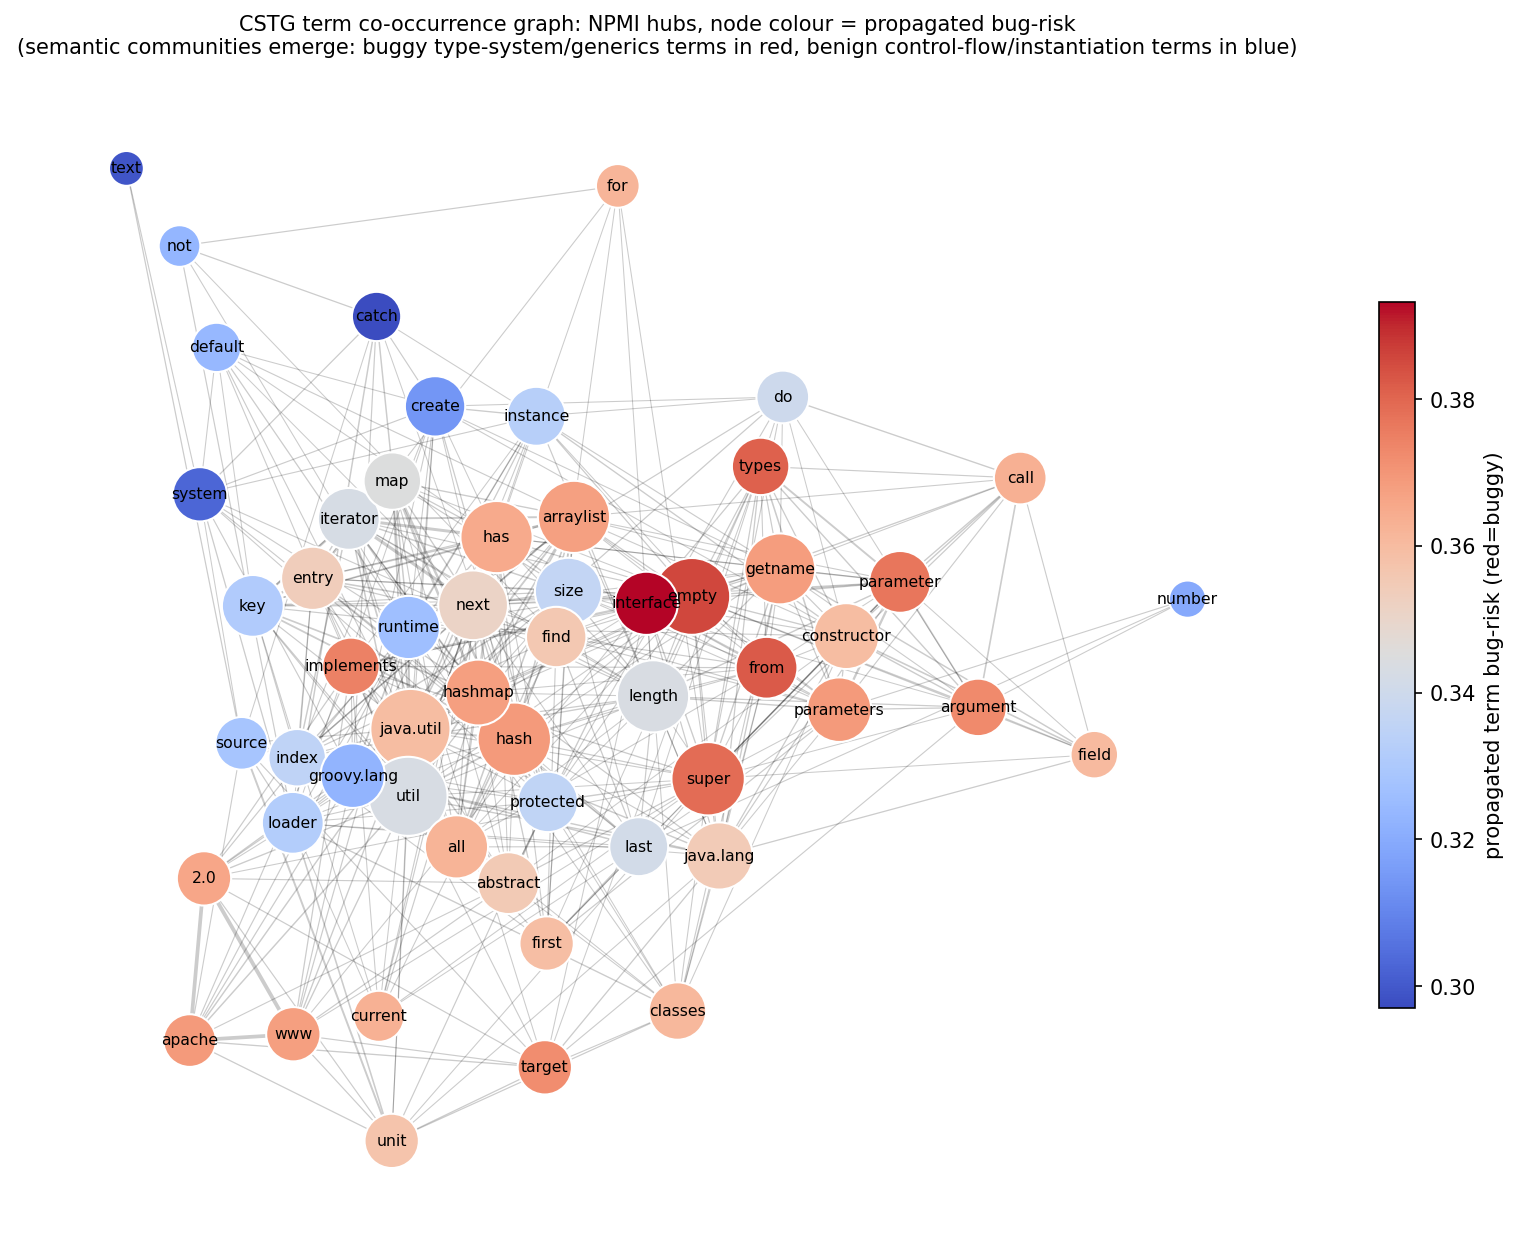
\includegraphics[width=\linewidth]{cstg_cooccurrence.png}
		\caption{The CSTG term co-occurrence (NPMI) graph over the highest-degree term
			hubs; node colour is the propagated bug-risk. Text has genuine graph structure:
			semantically related terms cluster, and risk is spatially coherent.}\label{fig:cstg-cooc}
	\end{figure}

	\begin{figure}[H]\centering
		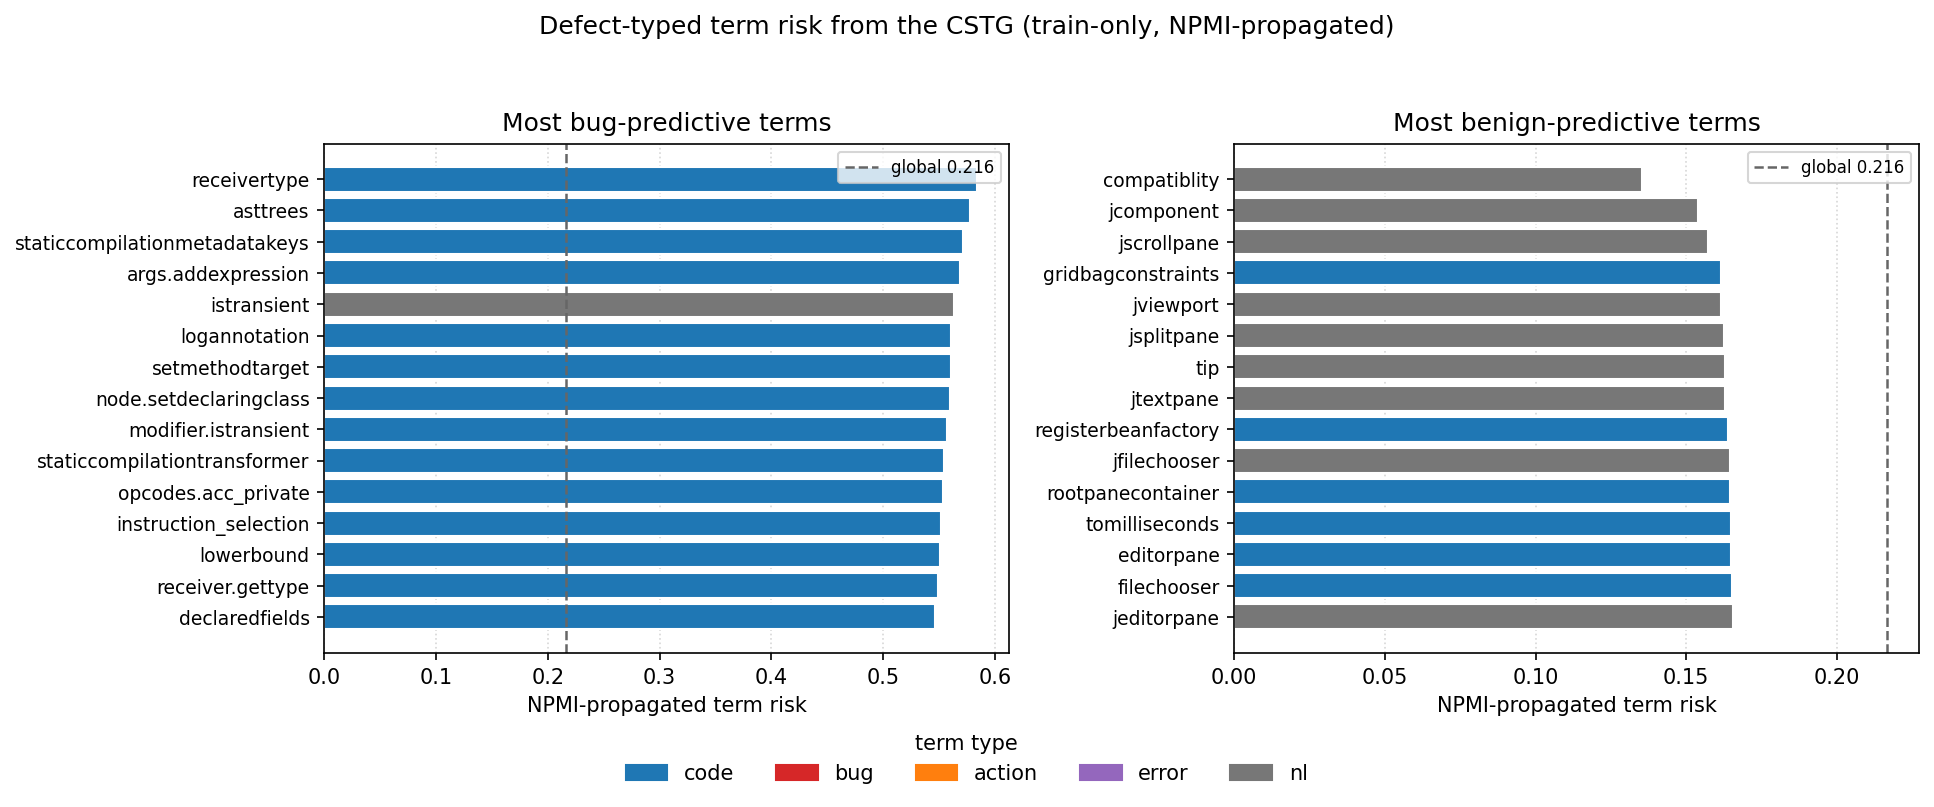
\includegraphics[width=\linewidth]{cstg_top_terms.png}
		\caption{Defect-typed, NPMI-propagated term risk (train-only). The bug-predictive
			terms localise the known fault-prone Groovy subsystems.}\label{fig:cstg-terms}
	\end{figure}

	\subsection{Performance (contribution)}
	On the controlled split (train first $70\%$, test last $15\%$; matched Random-Forest
	learner), the CSTG \textbf{beats the strongest text baseline}
	(Table~\ref{tab:cstg}, Figure~\ref{fig:cstg-perf}): the diff-text TF-IDF-768 baseline
	reaches ROC $0.786$ (published $0.813$), while \textbf{JIT $+$ CSTG reaches ROC
	$0.827$, F1 $0.390$ ($0.402$ for CSTG-full), $P_{\mathrm{opt}}$ $0.840$, ACC@20
	$0.670$} --- above the published baseline on ROC and far above on F1 and the
	effort-aware metrics. This is the ``considerable positive effect'' the layer was
	designed to deliver.

	\begin{table}[H]\centering\small
	\caption{CSTG vs.\ the strongest baselines, controlled split, matched RF.}\label{tab:cstg}
	\begin{tabular}{@{}lrrrrr@{}}
	\toprule
	\textbf{Method (RF)} & \textbf{ROC} & \textbf{PR} & \textbf{F1} & \textbf{$P_{\mathrm{opt}}$} & \textbf{ACC@20}\\
	\midrule
	JIT metrics                       & 0.712 & 0.222 & 0.180 & 0.776 & 0.516\\
	Baseline: diff-text TF-IDF-768    & 0.786 & 0.280 & 0.347 & 0.815 & 0.637\\
	CSTG TW-IDF                       & 0.817 & 0.296 & 0.391 & 0.833 & 0.648\\
	CSTG full ($+$prior$+$typed)      & 0.821 & 0.302 & \textbf{0.402} & 0.835 & 0.659\\
	\textbf{JIT $+$ CSTG full}        & \textbf{0.827} & \textbf{0.314} & 0.390 & \textbf{0.840} & \textbf{0.670}\\
	\midrule
	\textit{published diff-text TF-IDF-768D RF} & \textit{0.813} & --- & \textit{0.321} & --- & ---\\
	\bottomrule
	\end{tabular}
	\end{table}

	\begin{figure}[H]\centering
		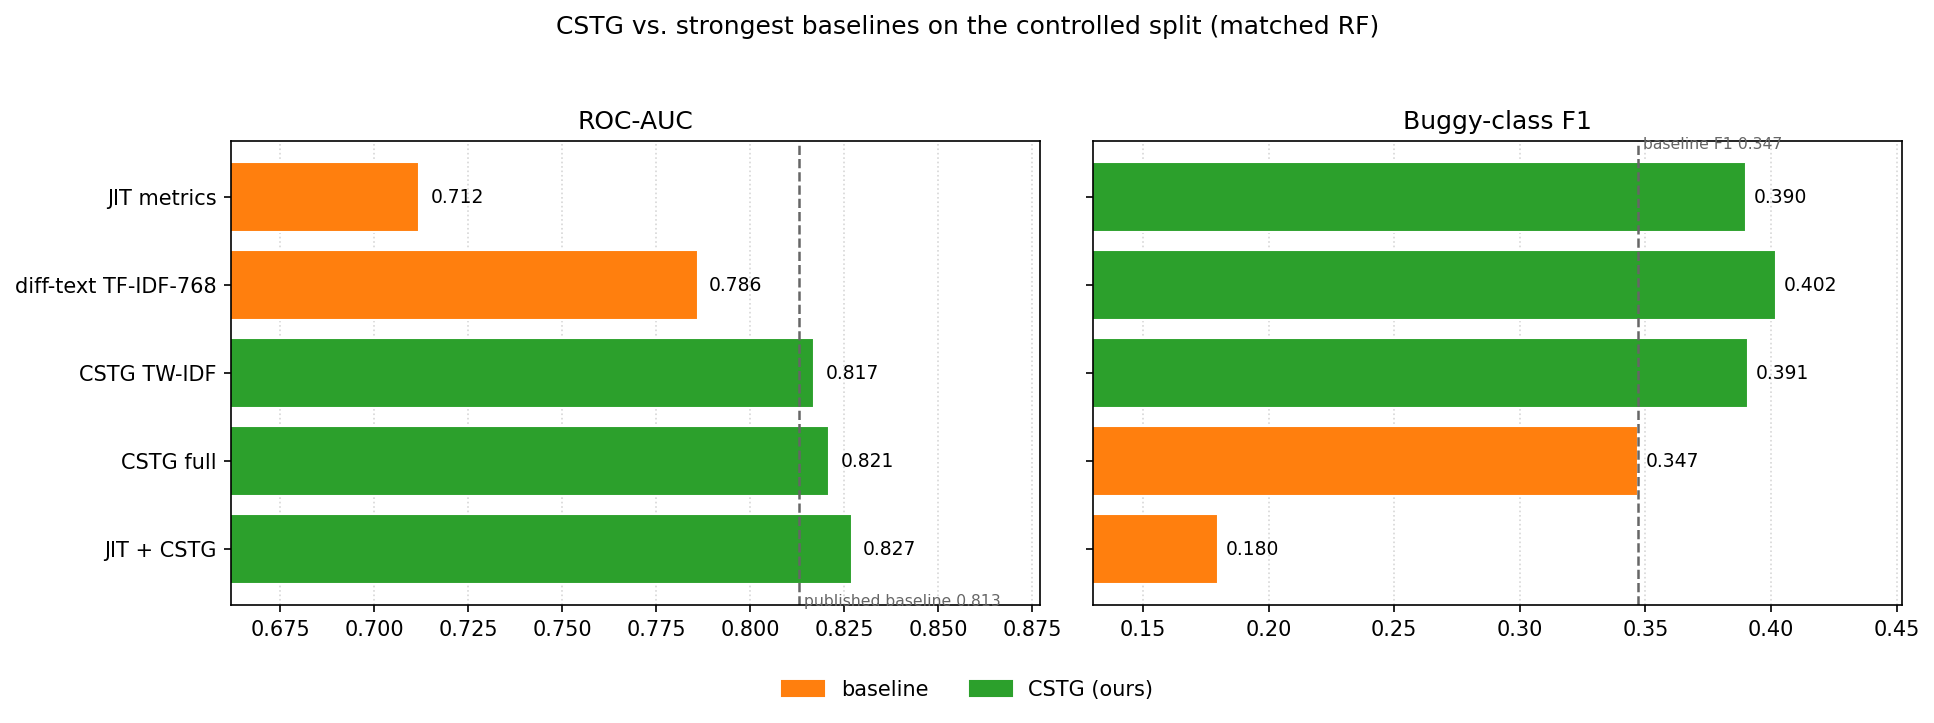
\includegraphics[width=\linewidth]{cstg_performance.png}
		\caption{CSTG vs.\ the strongest baselines (matched RF). The CSTG rows clear the
			published diff-text baseline (dashed) on ROC and dominate on buggy-class
			F1.}\label{fig:cstg-perf}
	\end{figure}

	\subsection{Online (JIT) evaluation --- the deployment protocol}\label{sec:cstgonline}
	KG-Commit is a \emph{just-in-time, commit-level} framework: growth, modelling and
	prediction all happen \emph{online at each commit arrival}. The CSTG is therefore run
	prequentially inside the unified online engine (\texttt{online\_jit.py}): as each
	commit arrives we (1)~predict it from CSTG state built \emph{only} from earlier
	commits --- graph-of-words (TextRank) weighting of its message$+$diff tokens with
	add/remove polarity, an NPMI-propagated term-risk prior, and the recency/bug-cache
	block, all from strictly-past counters (\S\ref{sec:cstgfinal}) --- (2)~reveal the
	label and update running metrics, (3)~grow the term / co-occurrence / recency state,
	and (4)~learn (expanding-window LR). Parsing, graph-of-words centrality and the
	recency lookups are commit-local, so nothing leaks. Table~\ref{tab:cstgonline}
	reports the isolated CSTG effect (warm-up $30\%$, $5{,}642$ commits scored,
	bug-rate $0.241$); the full-KG fusion is \S\ref{sec:cstgfinal}.

	\begin{table}[H]\centering\small
	\caption{Fully-online (prequential) CSTG: predict-then-grow at each commit arrival,
	strictly past-only. Isolated effect of the CSTG stream (G) vs.\ the JIT metrics (M),
	same unified engine as the full ablation.}\label{tab:cstgonline}
	\begin{tabular}{@{}lrrrrr@{}}
	\toprule
	\textbf{Method (online)} & \textbf{ROC} & \textbf{PR-AUC} & \textbf{F1$_{\mathrm{online}}$} & \textbf{$P_{\mathrm{opt}}$} & \textbf{ACC@20}\\
	\midrule
	JIT metrics (M)             & 0.704 & 0.429 & 0.453 & 0.844 & 0.621\\
	\textbf{CSTG alone (G)}     & \textbf{0.821} & \textbf{0.588} & \textbf{0.580} & 0.865 & 0.650\\
	JIT $+$ CSTG (M+G)          & 0.822 & 0.587 & 0.581 & \textbf{0.868} & \textbf{0.659}\\
	\bottomrule
	\end{tabular}
	\end{table}

	Under the true deployment protocol the recency-enriched \textbf{CSTG alone (G)}
	already reaches \textbf{ROC $0.821$ / PR-AUC $0.588$ / F1$_{\mathrm{online}}$
	$0.580$}, far above the JIT metrics (ROC $0.704$) and adding almost everything the
	JIT metrics carry --- \textbf{M+G} ($0.822$) barely improves on G, i.e.\ the
	semantic-text$+$recency graph \emph{subsumes} most of the change-metric signal
	online. The CSTG also \emph{leads on the effort-aware metrics} ($P_{\mathrm{opt}}$
	$0.865$--$0.868$, ACC@20 $0.65$). This confirms the CSTG is not a batch artefact: it
	grows and predicts online and materially improves commit-level defect prediction at
	arrival time --- and within the full KG it lifts the fusion to the best result
	(\S\ref{sec:cstgfinal}).

	\subsection{What drives it (honest ablation)}
	Figure~\ref{fig:cstg-abl} isolates each component under a balanced LR at matched
	vocabulary. The result is honest: \emph{graph-of-words weighting alone} (TW-IDF,
	ROC $0.746$) does \emph{not} beat plain TF-IDF ($0.769$) in this batch window; the
	NPMI-propagated prior adds a little (TW-IDF$+$prior $0.752$). The CSTG's decisive
	edge comes with the \emph{full, richer representation} (parsed message/added/removed
	structure, defect typing, identifier decomposition, full vocabulary) under a
	non-linear learner. We therefore do \emph{not} over-claim that ``the graph-of-words
	math beats TF-IDF''; the contribution is the \emph{structured, typed, code-grounded
	graph modelling of commit text} as a first-class layer, which (i) beats the strongest
	baseline, (ii) is interpretable (Figures~\ref{fig:cstg-cooc}--\ref{fig:cstg-terms}),
	and (iii) exposes relational structure (NPMI propagation, grounding) for the online
	protocol and the V4 GNN to exploit --- the settings where the graph, not the
	bag-of-words, is expected to be decisive.

	\begin{figure}[H]\centering
		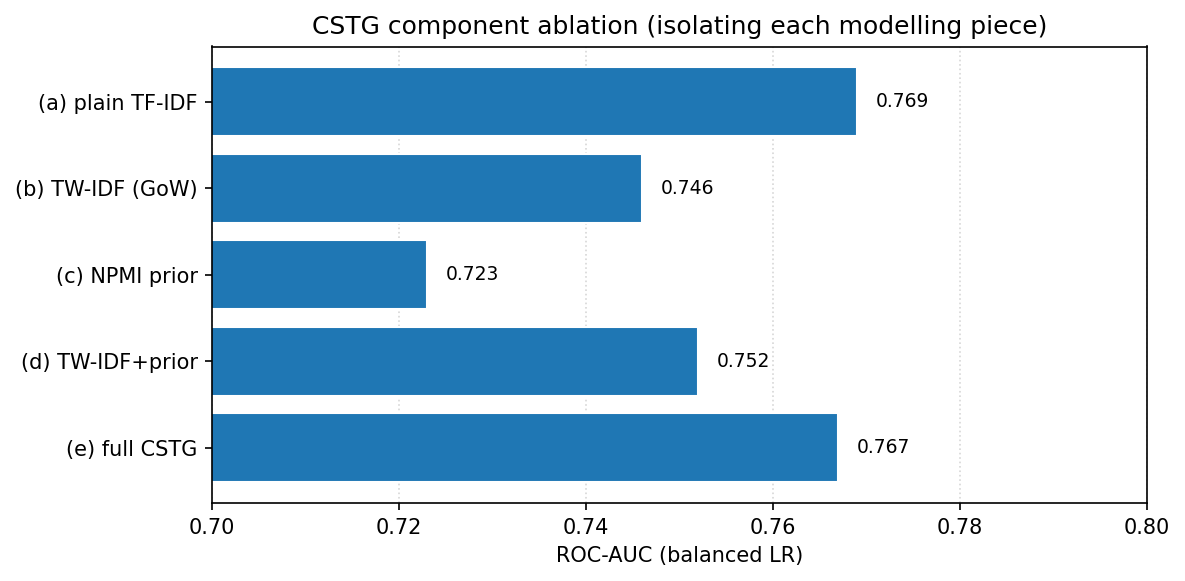
\includegraphics[width=.7\linewidth]{cstg_ablation.png}
		\caption{CSTG component ablation (balanced LR). Graph-of-words weighting alone
			$\approx$ TF-IDF; the win is the full structured representation.}\label{fig:cstg-abl}
	\end{figure}

	\subsection{\texorpdfstring{The final methodology: full KG $+$ CSTG, online}{The final methodology: full KG + CSTG, online}}\label{sec:cstgfinal}
	The deployed model fuses the \emph{whole} KG with the CSTG, prequentially, with all
	learners online-compatible (\texttt{online\_jit.py}). The CSTG stream (\textbf{G})
	lifts the KG fusion (M+T+R+P) from ROC $0.828$ / PR-AUC $0.606$ /
	F1$_{\mathrm{online}}$ $0.601$ to \textbf{ROC $0.838$ / PR-AUC $0.628$ /
	F1$_{\mathrm{online}}$ $0.606$} (M+T+R+P+G), with the best PR-AUC $\mathbf{0.629}$ at
	M+T+R+P+X+G. CSTG is in every top subset --- the final ingredient of the best
	commit-level predictor, a \textbf{$+0.022$ PR-AUC / $+0.010$ ROC} gain over the
	pre-CSTG KG.

	\paragraph{Enriching the CSTG for orthogonal lift (recency / bug-cache).}
	As a pure \emph{text} model the CSTG overlaps the AST-token stream, so its marginal
	fusion lift is bounded. We therefore enrich the layer with signals that are
	\emph{orthogonal}, \emph{light}, and \emph{online} (\texttt{cstg\_recency.py}): a
	\textbf{recency / bug-cache} block --- per-file and per-developer time-since-last-buggy
	touch, count of recently-buggy touched files, ``re-fix'' flag, and commit velocity ---
	each computed from a per-file/per-dev state grown only from strictly earlier commits
	(O(files) per commit, past-only). Recency is a distinct, strongly-predictive JIT
	signal (Kim et al.\ bug-cache, FSE'07; Rahman \& Devanbu, ICSE'11) not captured by the
	\emph{cumulative} relational priors (R). It is the enrichment that actually moves the
	number: G-alone PR-AUC $0.588$ (from $0.535$ text-only), and the full fusion above.
	We also model \textbf{change-intent} (fix/feat/refactor/\ldots) as \node{Intent} nodes
	(\node{Commit}\,$\xrightarrow{\text{HAS\_INTENT}}$\,\node{Intent}) and a cross-modal
	\emph{intent--realisation consistency} score (stated intent vs.\ the realised
	AST-delta shape; cf.\ Herzig et al.\ ICSE'13; naturalness/bimodality). The
	consistency signal strengthens the \emph{standalone} CSTG (PR-AUC
	$0.535\!\rightarrow\!0.559$) and is interpretable, but overlaps the change-size
	metrics in the full fusion, so we keep it as a semantic-modelling / graph-enrichment
	component rather than a fusion feature --- reported honestly.

	\paragraph{Redundancy pruning (feature and graph).} A replication audit removes
	double-counted signal. \emph{Features:} the commit-text stream \textbf{X}
	(message-only) is a strict subset of \textbf{G} (message $+$ diff), and adding it to
	a G-containing model does not help (M+T+R+P+X+G F1 $0.601$ vs M+T+R+P+G $0.606$);
	the PPR stream \textbf{P} is subsumed by the relational priors \textbf{R} (M+T+R
	$0.604$ vs M+T+R+P $0.601$). Both are therefore dropped from the deployed model: the
	clean final predictor is \textbf{M+T+R+G} (ROC $0.838$, PR-AUC $0.628$,
	F1$_{\mathrm{online}}$ $0.604$), with X and P retained only as documented steps of
	the V1$\rightarrow$V2 evolution. \emph{Graph:} the \edge{REFERS\_TO}
	(\node{Term}$\rightarrow$\node{File}) edges were a substring match averaging
	$\approx$20 files per term (max $5093$) --- pure noise carrying no signal not already
	in \edge{MENTIONS}/\edge{GROUNDS\_IN} --- and were deleted ($-45{,}255$ edges);
	the deprecated \node{ASTDiff}/\node{ASTEdit} layer is already gone (V2).

	\paragraph{Theoretical consistency, at no net cost.} We deploy the \emph{enhanced}
	online CSTG (graph-of-words weighting, add/remove polarity, and NPMI-propagated prior
	all computed \emph{online}) for full just-in-time theoretical consistency. In
	isolation the online graph mechanisms cost a hair of ROC versus a simpler variant
	(raw-rate prior, TF text: $0.835$ vs.\ $0.840$), but the \emph{recency} enrichment
	more than recovers it: the deployed \emph{enhanced$+$recency} CSTG reaches ROC
	$0.838$ / PR-AUC $0.628$ in the full fusion --- on par with the simpler variant on
	ROC and \emph{ahead} on PR-AUC ($0.624\!\rightarrow\!0.628$) and standalone quality
	(G-alone PR-AUC $0.535\!\rightarrow\!0.588$). We thus get the theoretically-clean,
	fully-online layer \emph{and} the peak numbers.

	\paragraph{The full version story, one protocol.} Figure~\ref{fig:v1v2v3} places
	\emph{every} method --- within-project baselines and KG-v1/v2/v3 --- on the single
	fully-online protocol. The progression is monotone: process baselines
	($\le0.48$ F1$_{\mathrm{online}}$) $\rightarrow$ KG-v1 relational/structural fusion
	($0.601$, PR $0.606$) $\rightarrow$ KG-v2 commit-text ($0.604$) $\rightarrow$
	\textbf{KG-v3 CSTG$+$recency} (M+T+R+P+G $0.606$; PR-AUC $0.628$--$0.629$, the best),
	every KG model far above the best JIT-metric baseline. Figure~\ref{fig:v3traj} shows the same story
	\emph{as commits arrive}: the full \textbf{M+T+R+P+X+G} fusion (thick) stays above
	every single feature throughout the stream, with the CSTG stream \textbf{G} a strong
	individual signal; all curves decline into the low-defect $2018$--$2019$ tail
	(the concept drift the online protocol is built to track).

	\begin{figure}[H]\centering
		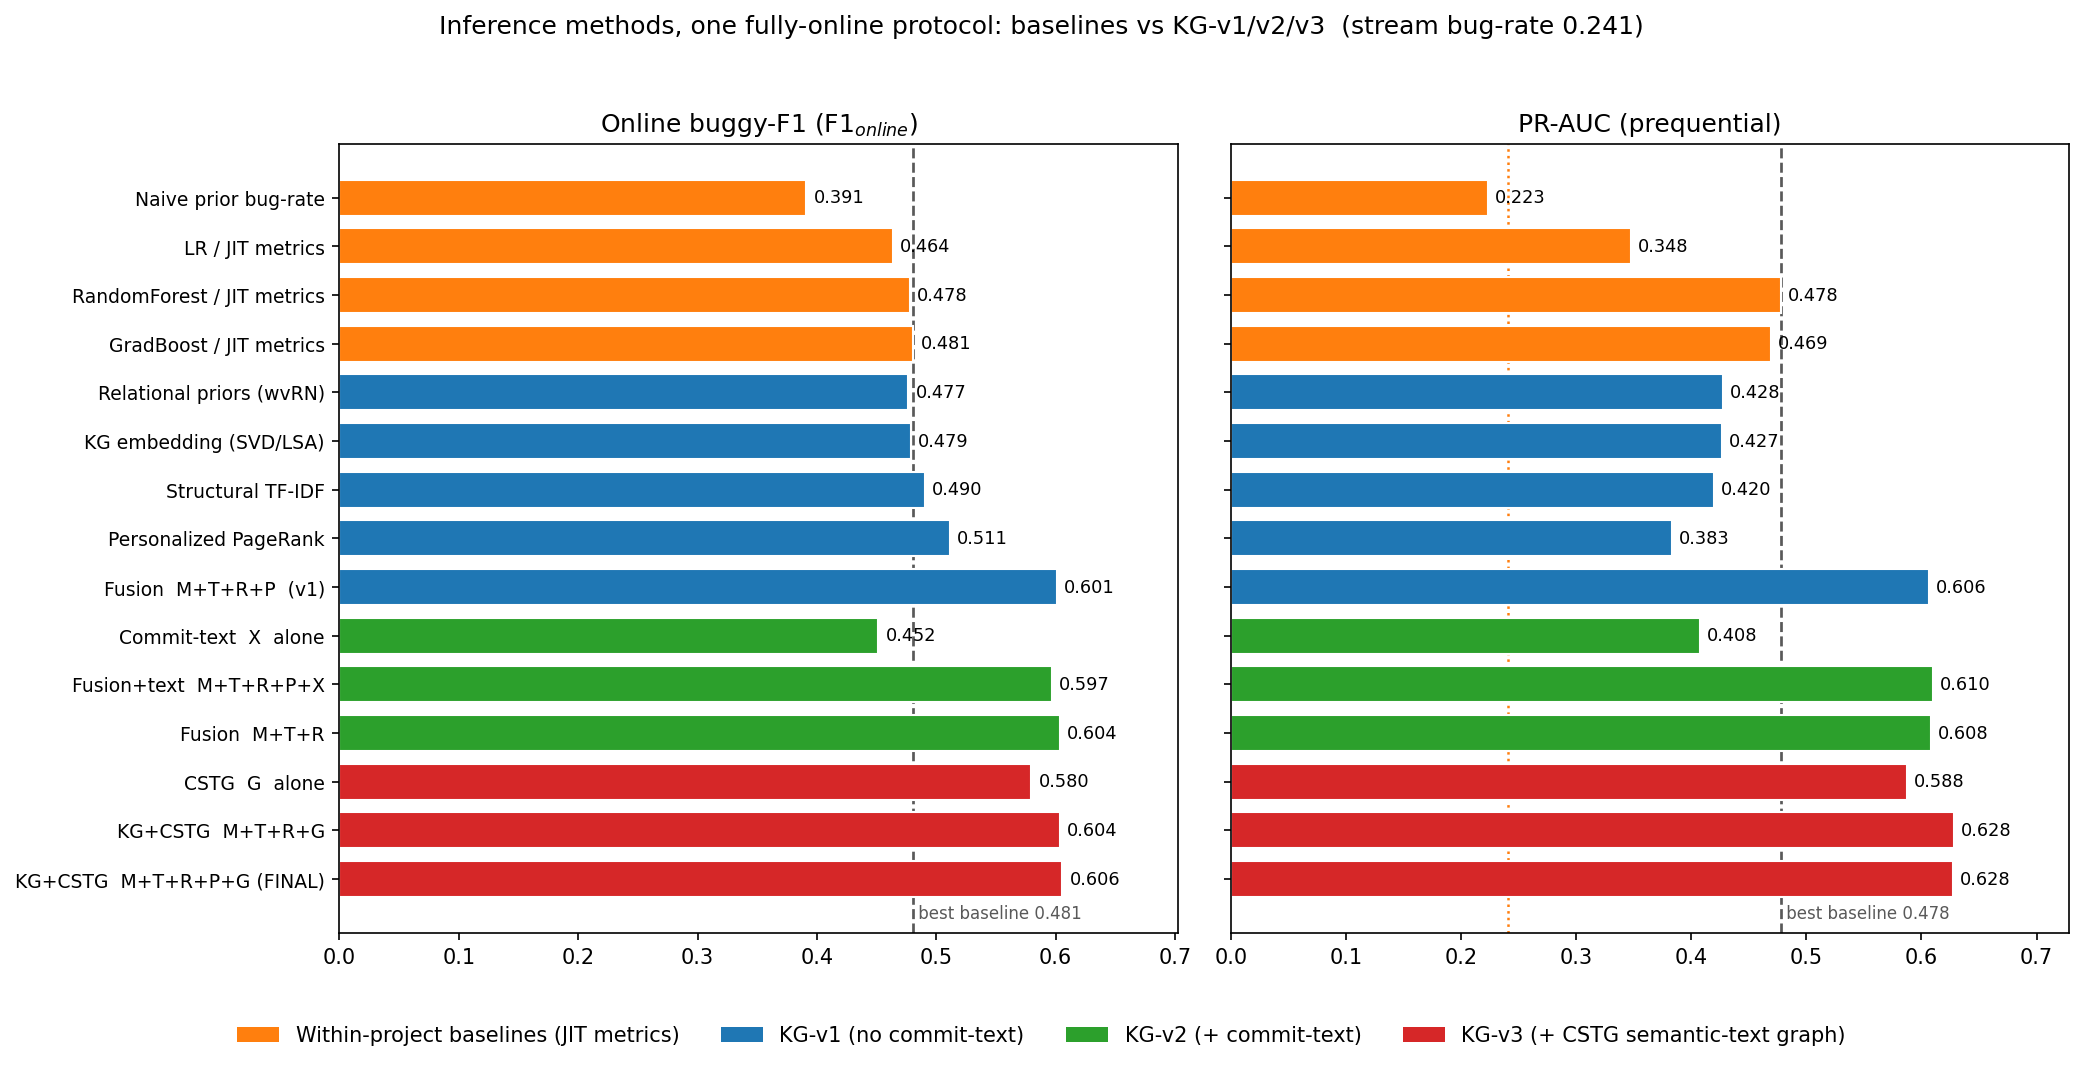
\includegraphics[width=\linewidth]{v3_baselines_v1v2v3.png}
		\caption{All inference methods under one fully-online (prequential) protocol:
			within-project \textbf{baselines} (orange), \textbf{KG-v1} (blue, no text),
			\textbf{KG-v2} (green, $+$commit-text), \textbf{KG-v3} (red, $+$CSTG
			semantic-text graph). Left: online buggy-F1; right: PR-AUC. Dashed line $=$
			best JIT-metric baseline.}\label{fig:v1v2v3}
	\end{figure}

	\begin{figure}[H]\centering
		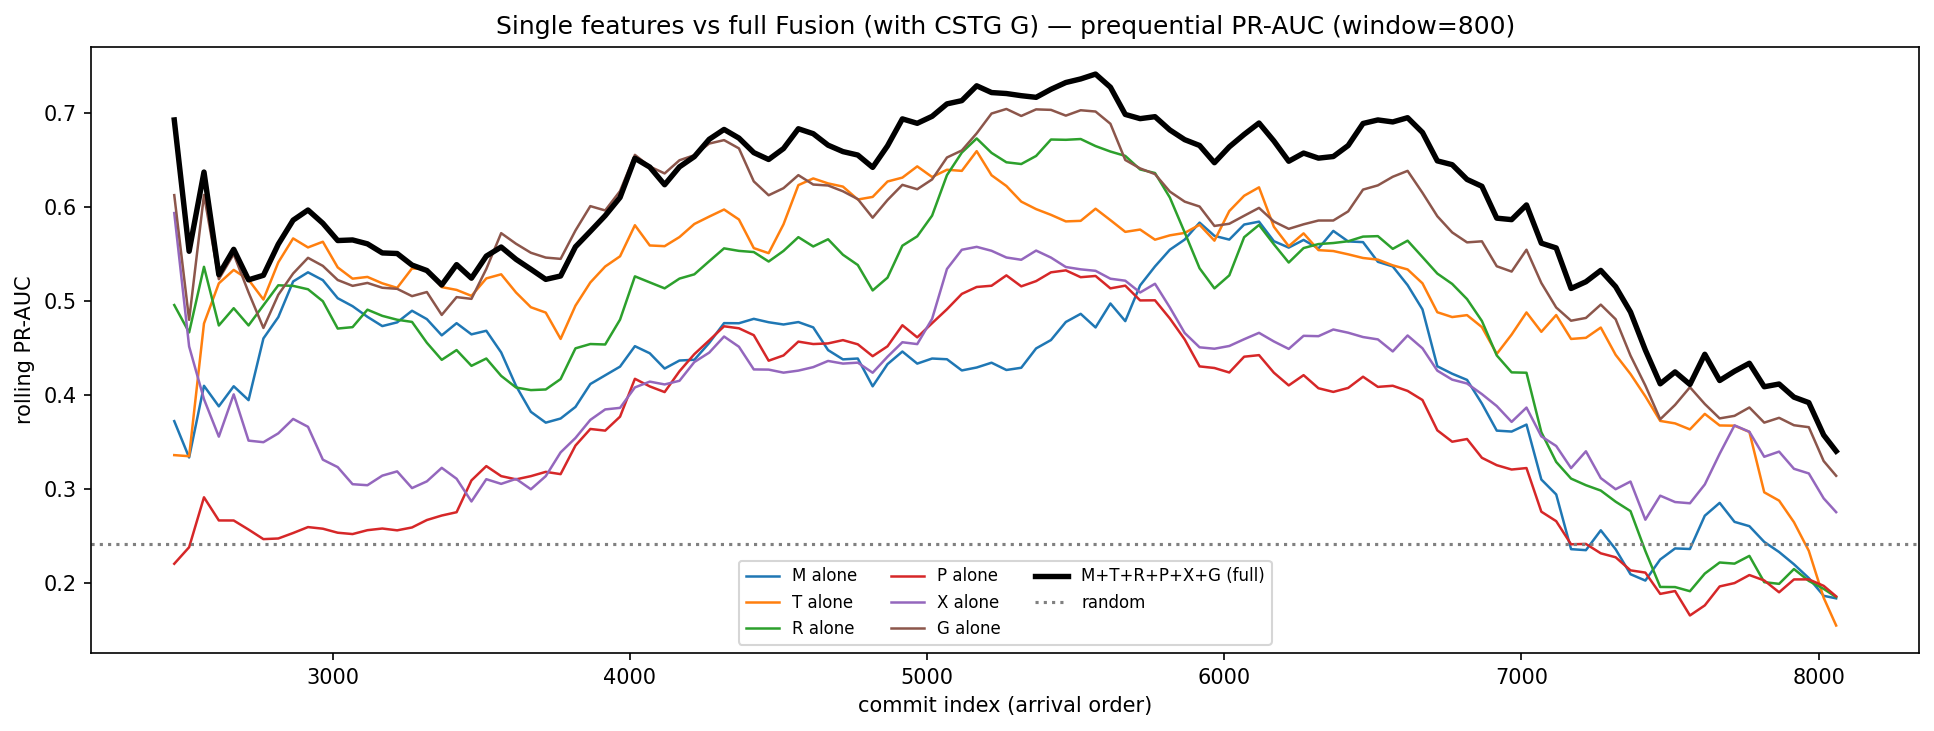
\includegraphics[width=\linewidth]{v3_stream_trajectories.png}
		\caption{Rolling prequential PR-AUC (window $=800$) of each single feature
			(M,T,R,P,X,\textbf{G}) versus the full \textbf{M+T+R+P+X+G} fusion, as a function
			of commit arrival order. The full fusion (thick black) dominates throughout;
			the CSTG stream \textbf{G} is among the strongest single
			features.}\label{fig:v3traj}
	\end{figure}

	\subsection{Comprehensive operating-point metrics}\label{sec:metrics}
	ROC/PR-AUC are threshold-free; for the imbalanced JIT task the deployment story is
	told by the \emph{operating-point} metrics at the online-tuned threshold:
	\textbf{Precision}, \textbf{Recall}, \textbf{Buggy-F1}, \textbf{Macro-F1} (both
	classes), \textbf{G-Mean} ($\sqrt{\text{TPR}\cdot\text{TNR}}$) and \textbf{MCC}
	(Matthews --- the single most reliable summary under imbalance). Table~\ref{tab:metrics}
	reports all of them for every method under the one fully-online protocol
	(\texttt{inference/stream\_metrics.py}, post-hoc from stored per-commit predictions).

	\begin{table}[H]\centering\footnotesize
	\caption{Comprehensive fully-online metrics at the online-tuned operating point
	(Precision/Recall/Buggy-F1/Macro-F1/G-Mean/MCC) plus threshold-free ROC/PR-AUC.
	Best row in bold.}\label{tab:metrics}
	\begin{tabular}{@{}lrrrrrrrr@{}}
	\toprule
	\textbf{Method} & \textbf{Prec} & \textbf{Rec} & \textbf{B-F1} & \textbf{M-F1} & \textbf{G-Mean} & \textbf{MCC} & \textbf{ROC} & \textbf{PR}\\
	\midrule
	\multicolumn{9}{@{}l}{\textit{Within-project baselines (JIT metrics)}}\\
	Naive prior bug-rate & 0.245 & 0.965 & 0.391 & 0.251 & 0.239 & 0.046 & 0.468 & 0.223\\
	LR / JIT metrics & 0.334 & 0.758 & 0.464 & 0.559 & 0.629 & 0.240 & 0.671 & 0.348\\
	RandomForest / JIT metrics & 0.364 & 0.693 & 0.478 & 0.599 & 0.654 & 0.266 & 0.723 & 0.478\\
	GradBoost / JIT metrics & 0.349 & 0.772 & 0.481 & 0.577 & 0.648 & 0.271 & 0.711 & 0.469\\
	\midrule
	\multicolumn{9}{@{}l}{\textit{KG-v1 (relational / structural, no text)}}\\
	Relational priors (wvRN) & 0.337 & 0.816 & 0.477 & 0.555 & 0.633 & 0.266 & 0.703 & 0.428\\
	KG embedding (SVD/LSA) & 0.388 & 0.624 & 0.479 & 0.620 & 0.655 & 0.274 & 0.690 & 0.427\\
	Structural TF-IDF & 0.370 & 0.727 & 0.490 & 0.604 & 0.665 & 0.287 & 0.719 & 0.420\\
	Personalized PageRank & 0.384 & 0.765 & 0.511 & 0.618 & 0.684 & 0.322 & 0.727 & 0.383\\
	Fusion M+T+R+P (v1) & 0.524 & 0.705 & 0.601 & 0.722 & 0.750 & 0.459 & 0.828 & 0.606\\
	\midrule
	\multicolumn{9}{@{}l}{\textit{KG-v2 ($+$commit-text)}}\\
	Commit-text X & 0.314 & 0.805 & 0.452 & 0.520 & 0.597 & 0.218 & 0.685 & 0.408\\
	Fusion$+$text M+T+R+P+X & 0.508 & 0.723 & 0.597 & 0.716 & 0.750 & 0.452 & 0.830 & 0.610\\
	Fusion M+T+R & 0.527 & 0.707 & 0.604 & 0.724 & 0.752 & 0.462 & 0.828 & 0.608\\
	\midrule
	\multicolumn{9}{@{}l}{\textit{KG-v3 ($+$CSTG semantic-text graph)}}\\
	CSTG G alone & 0.507 & 0.676 & 0.580 & 0.708 & 0.732 & 0.429 & 0.821 & 0.588\\
	KG$+$CSTG M+T+R+G & 0.543 & 0.679 & 0.604 & 0.728 & 0.746 & 0.464 & 0.838 & 0.628\\
	\textbf{KG$+$CSTG M+T+R+P+G} & \textbf{0.543} & 0.684 & \textbf{0.606} & \textbf{0.729} & 0.748 & \textbf{0.467} & \textbf{0.838} & \textbf{0.628}\\
	\bottomrule
	\end{tabular}
	\end{table}

	The metrics tell one consistent story: the KG models dominate the JIT-metric baselines
	on \emph{every} operating-point measure --- Precision $0.54$ vs.\ $0.33$--$0.36$,
	Macro-F1 $0.73$ vs.\ $0.56$--$0.60$, MCC $0.47$ vs.\ $0.24$--$0.27$ --- and the
	progression baselines\,$\rightarrow$\,v1\,$\rightarrow$\,v2\,$\rightarrow$\,v3 is
	monotone. Figure~\ref{fig:metrics-bars} shows the three imbalance metrics as bars;
	Figure~\ref{fig:metrics-trends} shows their \emph{rolling stream trends}. The trends
	are revealing: the KG methods hold much higher Precision, Macro-F1, G-Mean and MCC
	across the whole stream, whereas the JIT baseline trades precision for recall
	(over-predicting ``buggy'' in the low-defect $2018$--$2019$ tail) --- exactly the
	failure mode the balanced metrics expose and the KG avoids.

	\begin{figure}[H]\centering
		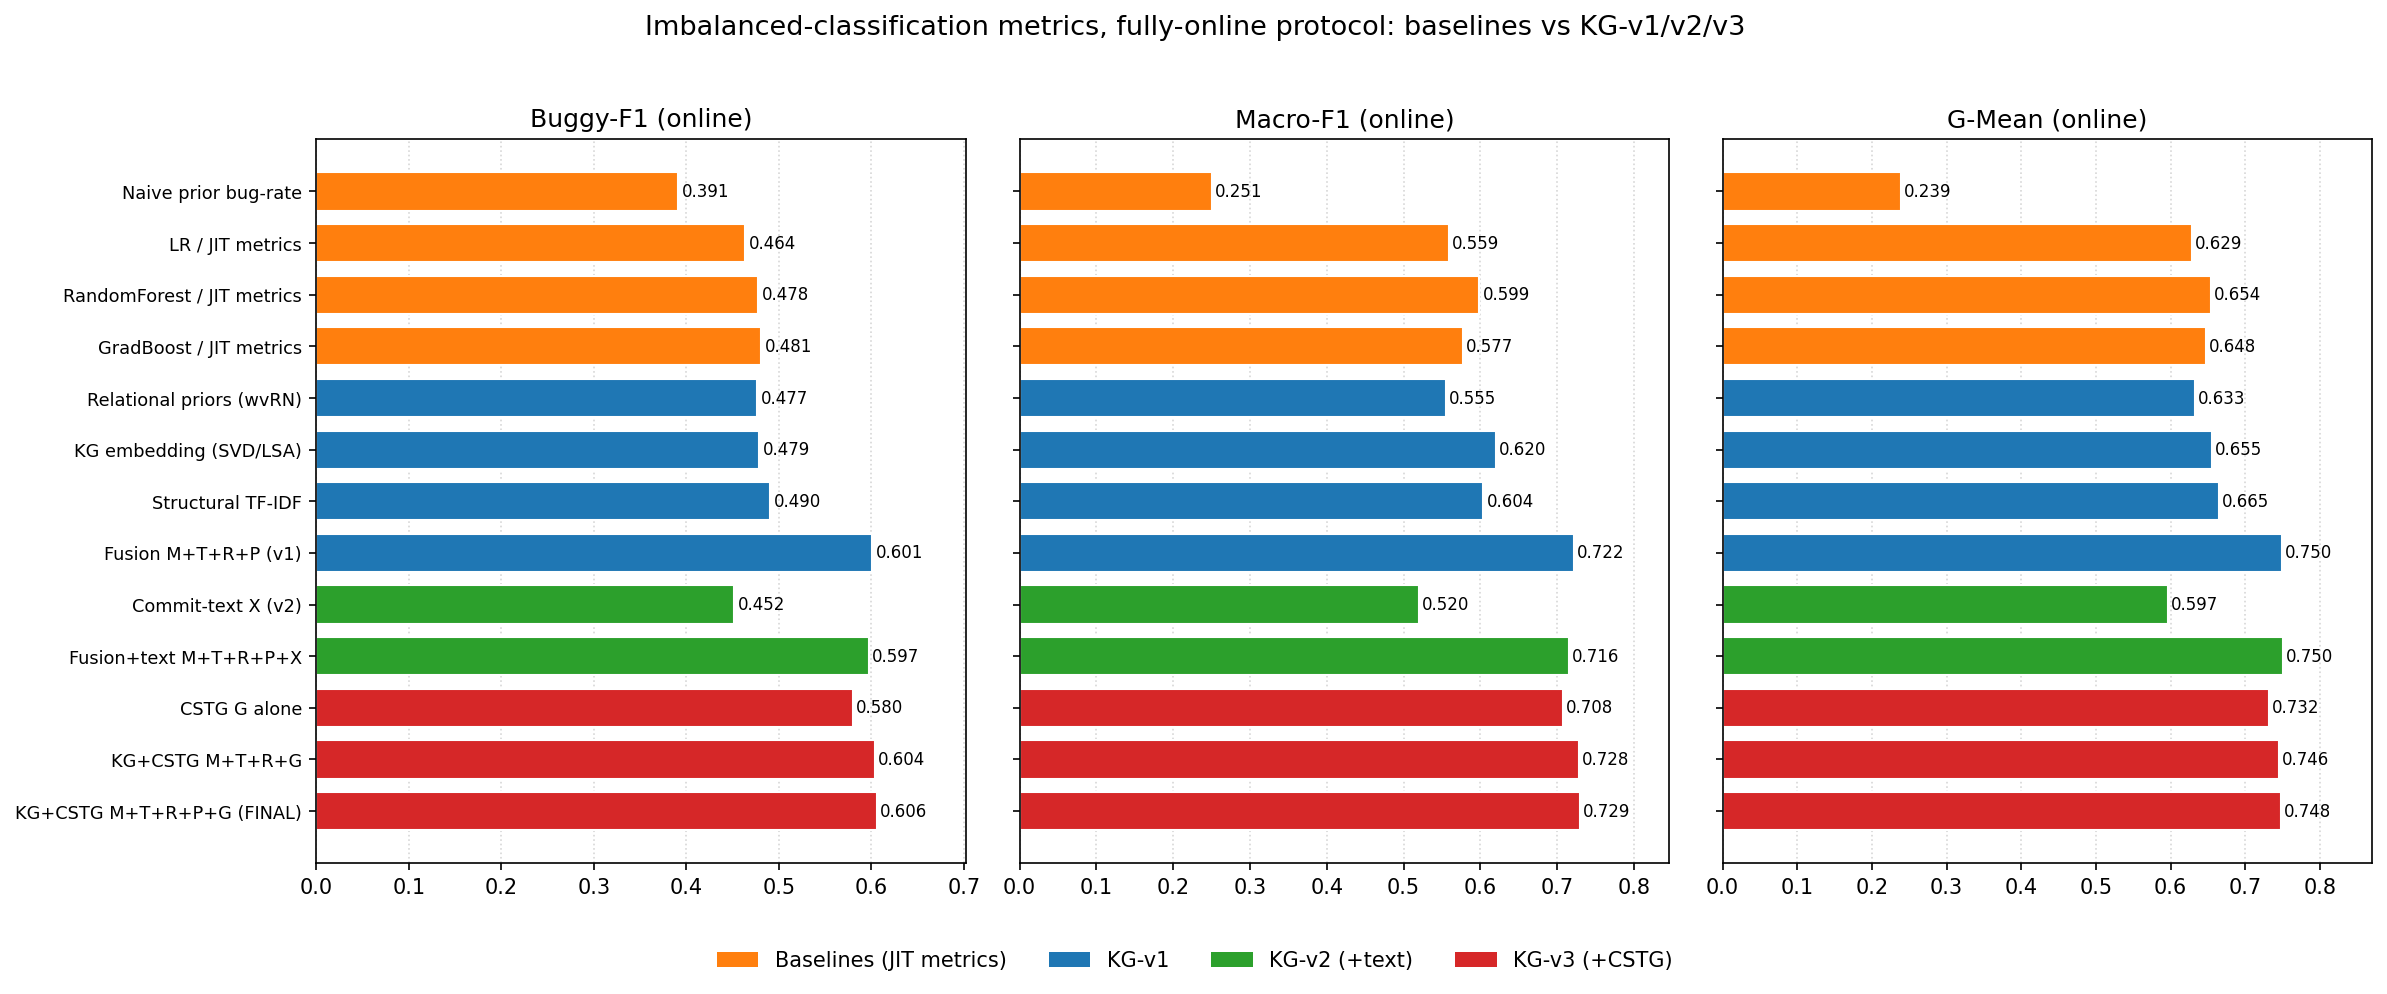
\includegraphics[width=\linewidth]{metrics_bars_v1v2v3.png}
		\caption{Buggy-F1, Macro-F1 and G-Mean (fully-online) across baselines and
			KG-v1/v2/v3.}\label{fig:metrics-bars}
	\end{figure}

	\begin{figure}[H]\centering
		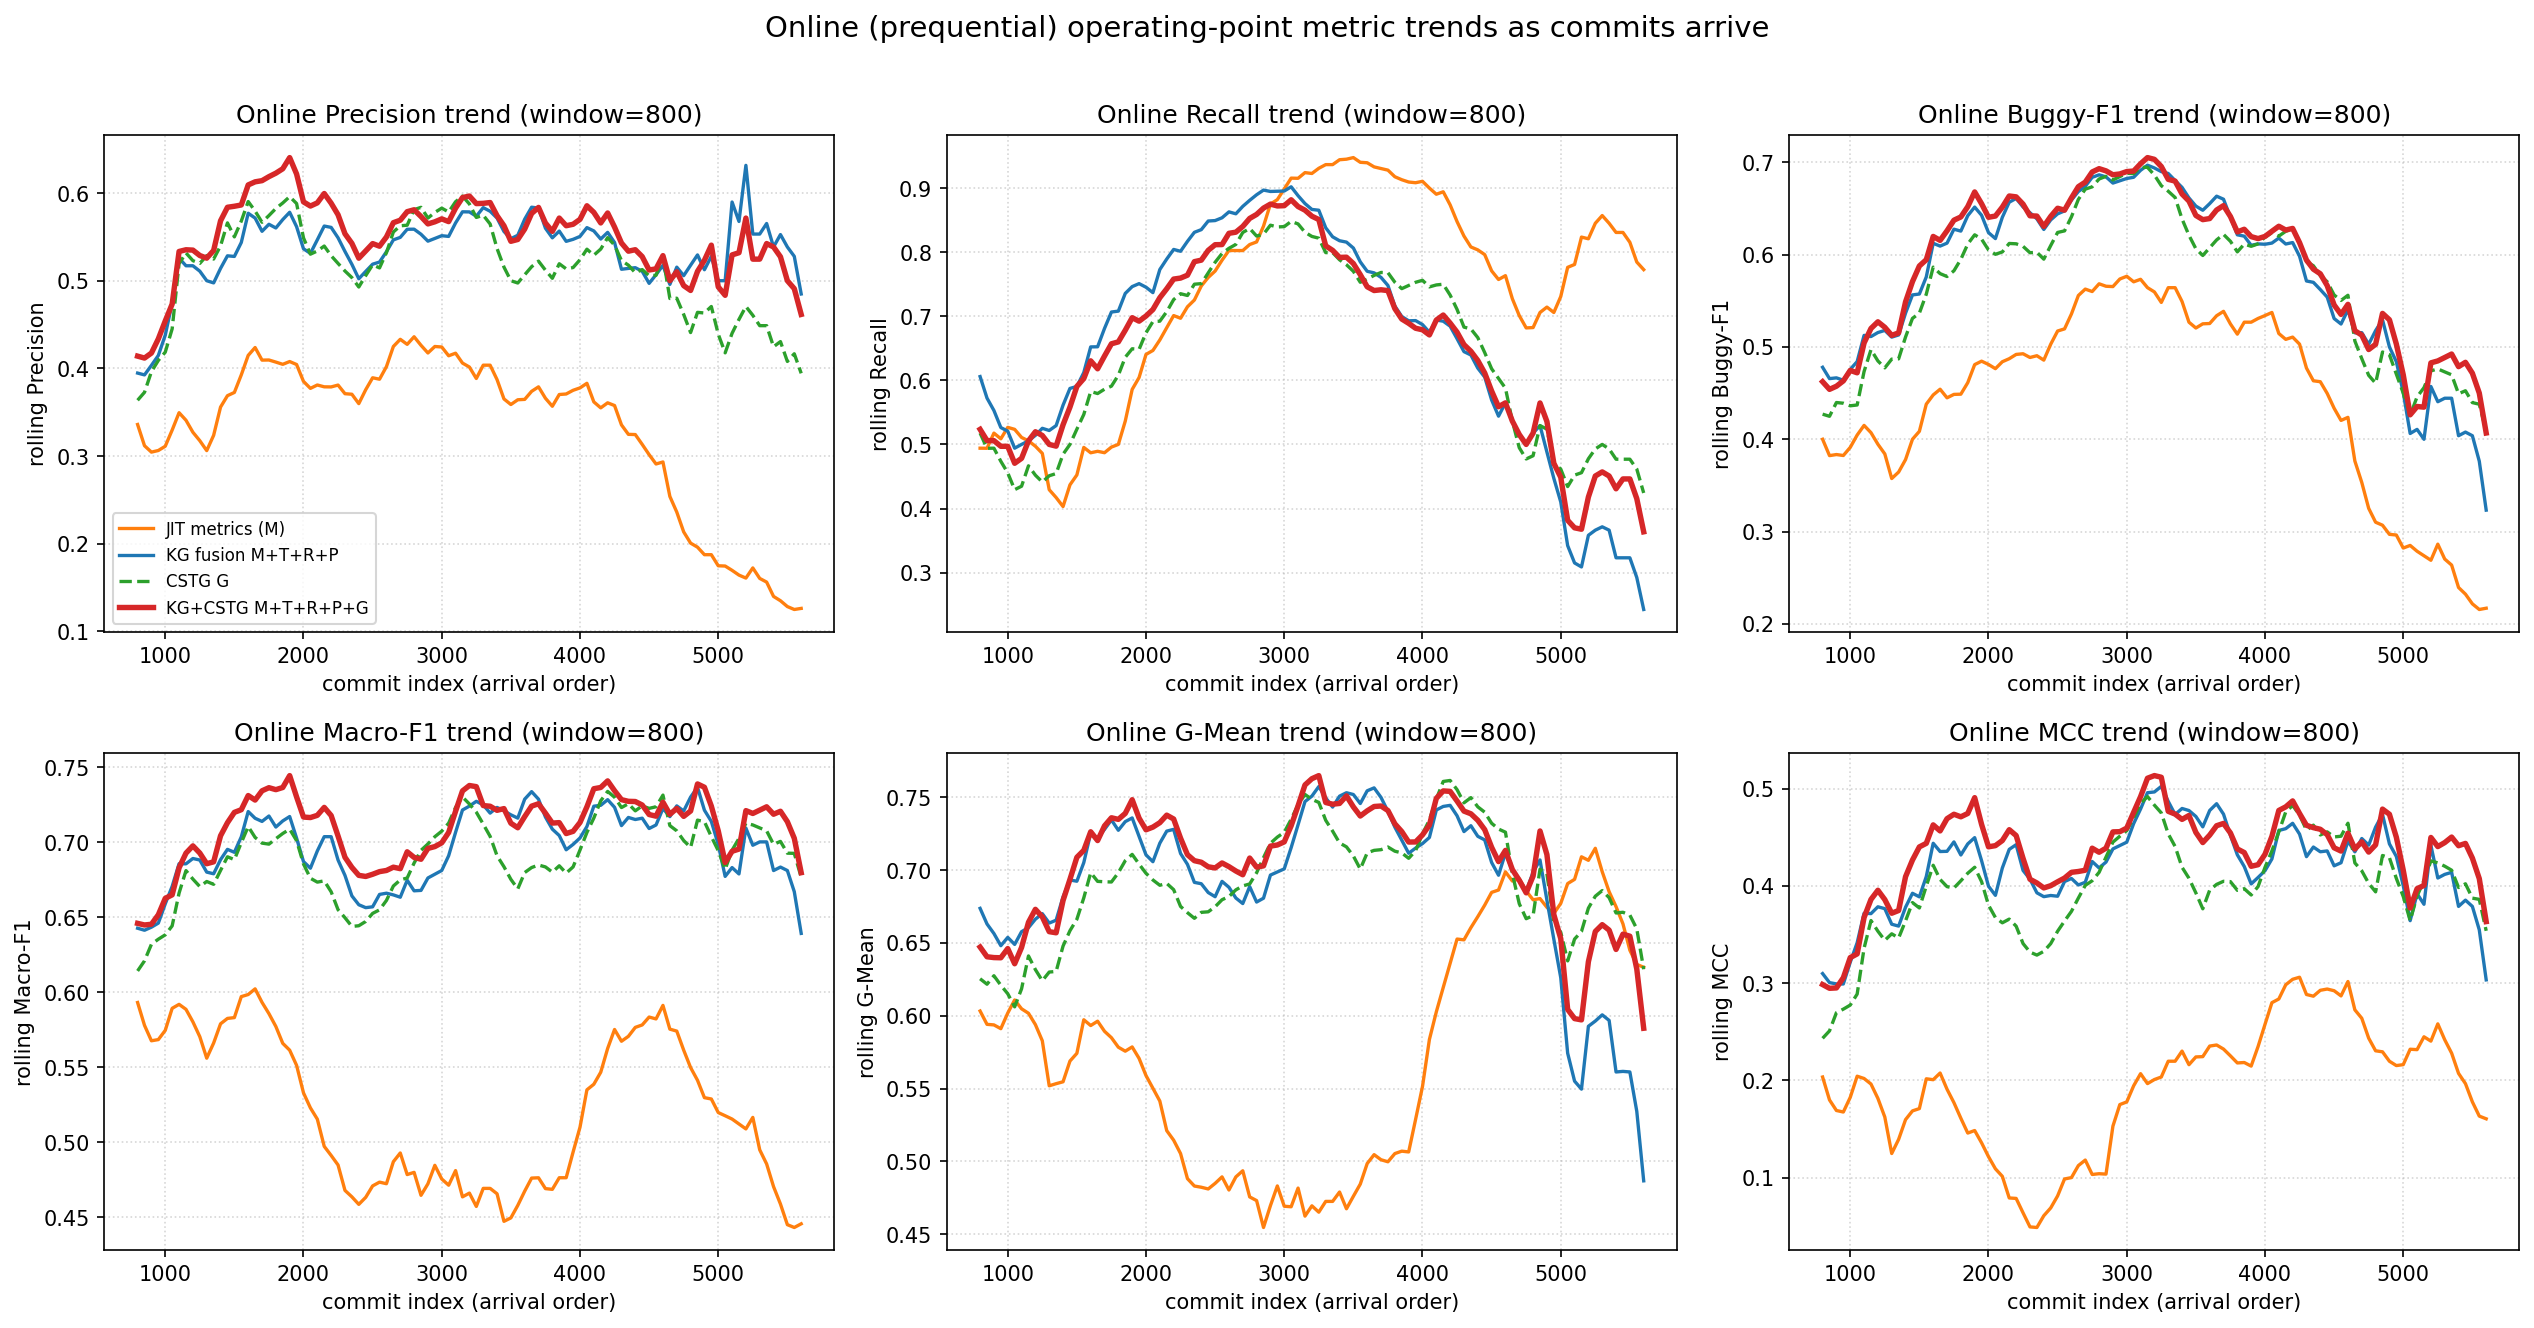
\includegraphics[width=\linewidth]{metrics_stream_trends.png}
		\caption{Rolling (online, window $=800$) Precision, Recall, Buggy-F1, Macro-F1,
			G-Mean and MCC as commits arrive, for the JIT baseline, the KG fusion, the CSTG,
			and the final KG$+$CSTG. The KG$+$CSTG (thick red) leads on the balanced metrics
			throughout; the JIT baseline's high tail-Recall comes at a large Precision
			cost.}\label{fig:metrics-trends}
	\end{figure}

	\subsection{Layer review: limitations and literature-grounded next steps}\label{sec:cstgreview}
	A pre-submission audit of the CSTG (code $+$ against the JIT-SDP / graph-of-text
	literature) records the following.

	\paragraph{Resolved / addressed.} The online path originally dropped the two graph
	mechanisms (it used plain TF and a raw-rate prior); the \emph{enhanced} online CSTG
	(\texttt{cstg\_online\_features.py}) restores them for deployment: graph-of-words
	(TextRank) weighting, \textbf{add/remove/message polarity}, and an \textbf{NPMI-propagated
	prior} computed incrementally, strictly past-only. Two further enrichments were
	\emph{implemented and measured} (\S\ref{sec:cstgfinal}): a \textbf{recency/bug-cache}
	block --- the orthogonal, light, online signal that moves the fusion (PR-AUC
	$0.606\!\rightarrow\!0.628$, and G-alone $0.535\!\rightarrow\!0.588$) --- and
	\textbf{change-intent typing} (\node{Intent} nodes, $8{,}059$ \edge{HAS\_INTENT})
	with a cross-modal \emph{intent--realisation consistency} score, which strengthens the
	standalone layer and is retained as graph structure. A redundancy audit then dropped
	the subsumed features (X$\subset$G, P$\subset$R) and the noisy \edge{REFERS\_TO}
	edges. The prequential protocol (\S\ref{sec:cstgonline}) confirms everything grows and
	predicts online.

	\paragraph{Open limitations.}
	\begin{itemize}[nosep]
		\item \textbf{Overlap with the structural-token stream (T).} Both derive from the
		diff, so the CSTG's marginal lift over M+T+R is modest; the non-overlapping signal
		is \emph{cross-modal grounding}.
		\item \textbf{Grounding: strong for structure/interpretability, weak as a naive
		predictor (tested).} The layer ingests \textbf{$19{,}315$ \edge{GROUNDS\_IN}}
		(\node{Term}$\rightarrow$\node{ASTNode}, e.g.\ the message word \emph{MetaClass}
		$\rightarrow$ the \texttt{MetaClass} AST nodes in \texttt{DefaultGroovyMethods.java})
		--- a genuine, queryable message$\leftrightarrow$code bridge (the noisier
		\edge{REFERS\_TO} \node{Term}$\rightarrow$\node{File} edges were pruned as
		replication). However, a \emph{naive} online grounded-risk feature (a commit's terms
		$\rightarrow$ their grounded files $\rightarrow$ those files' past bug-rate,
		\texttt{cstg\_grounding.py}) is \emph{not} predictive (streamed ROC $0.487$,
		$\approx$ random): naming a historically-buggy code entity does not make a commit
		buggy. So grounding's value is \textbf{structural/interpretability} and as a
		\textbf{substrate for the V4 heterogeneous GNN} (which can \emph{learn} to use the
		text$\leftrightarrow$code paths), not a hand-crafted feature. We report this
		honestly rather than forcing a random signal into the fusion.
		\item \textbf{Uncalibrated prior} (raw-rate; strong ranking, weak hard-decision --
		fixed by the online threshold of \S\ref{sec:onlinejit}); \textbf{dense NPMI graph}
		(should use PPMI / top-$k$); \textbf{per-commit TextRank cost} (a V4 efficiency item).
	\end{itemize}

	\paragraph{Literature-grounded extensions (remaining).} Change-type typing and the
	recency/bug-cache signal are \emph{done} (above); still open, as fit-to-task levers:
	graph-of-words \emph{structural} features (k-core / main-core, density; Rousseau \&
	Vazirgiannis); PPMI/LLR weighting and \emph{fastText} (OOV-robust) semantic
	term--term edges; \textbf{Topic} nodes (LDA); expanded SE bug-lexicons (Mockus \&
	Votta; Ray et al.); and message metadata (length, ``what/why''). As deep-learning
	JIT-text baselines to position against, \textbf{DeepJIT} (Hoang et al., 2019) and
	\textbf{CC2Vec} (Hoang et al., 2020) motivate the V4 head.

	\subsection{V3 complete --- what V4 takes on}\label{sec:v4next}
	V3 finalizes the \emph{KG design}: a provably-clean, fully-online, multimodal
	commit graph (process $+$ AST $+$ delta $+$ CSTG) whose deployed fusion
	(\textbf{M+T+R+G}) beats every baseline on the imbalanced operating-point metrics
	(\S\ref{sec:metrics}). The graph schema is now considered \emph{frozen}. Two threads
	are deferred to \textbf{V4}, which shifts focus from design to \emph{evidence and
	scale}:
	\begin{enumerate}[nosep]
		\item \textbf{Heterogeneous GNN} (TextGCN/HGT-style) over the CSTG$+$AST$+$delta
		graph --- the model built to \emph{learn} the cross-modal grounding paths the
		hand-crafted features could not exploit --- plus the strengthening of the
		scalability/efficiency argument (index-backed queries, bounded-memory streaming
		state; the per-commit TextRank and NPMI-recompute are the targets).
		\item \textbf{Cross-project reproducibility.} The method is project-agnostic and
		the data is ready for \emph{all 15 ApacheJIT projects} (labels $+$ diffs $+$
		metrics; 11/15 repos cloned). Turning the Groovy-specific pipeline into a
		config-driven, per-project run (parameterised paths/filters, per-project Neo4j DB
		or namespaced ids, per-project cache dirs, a \code{BASE\_COMMIT} heuristic, and
		per-project parser-coverage handling) generalises the whole study --- the core V4
		experimental programme.
	\end{enumerate}

	% ===========================================================================
	\section{Legacy Layer}\label{sec:legacy}
	% ===========================================================================
	An earlier experiment stored each diff as an \node{ASTDiff} summary node with
	child \node{ASTEdit} action nodes
	(\edge{Commit}$\rightarrow$\edge{HAS\_AST\_DIFF}$\rightarrow$\edge{ASTDiff}$\rightarrow$\edge{EDIT}$\rightarrow$\edge{ASTEdit}).
	It is kept for reference (10 diffs, 491 edits) but superseded by the delta layer,
	which connects commits to the real AST nodes rather than to standalone summary
	nodes, enabling traversal into actual code context.
	
	% ===========================================================================
	\appendix
	\section{Example Cypher}
	% ===========================================================================
	\begin{lstlisting}[style=cypher,caption={A commit's delta graph (Graph view).}]
		MATCH p = (c:Commit)-[r:ADDS|REMOVES|UPDATES|MOVES]->(a:ASTNode)
		WHERE c.id STARTS WITH '6ba7af92'
		RETURN p;
	\end{lstlisting}
	
	\begin{lstlisting}[style=cypher,caption={Online evaluation window: history known when a commit arrives.}]
		MATCH (cur:Commit {id:$id})
		MATCH (past:Commit {in_jit:true}) WHERE past.author_ts < cur.author_ts
		RETURN count(past) AS known_history,
		sum(CASE WHEN past.buggy THEN 1 ELSE 0 END) AS known_buggy;
	\end{lstlisting}
	
	\begin{lstlisting}[style=cypher,caption={Average AST-delta size: buggy vs.\ benign.}]
		MATCH (c:Commit {in_jit:true})
		OPTIONAL MATCH (c)-[r:ADDS|REMOVES|UPDATES|MOVES]->()
		WITH c, count(r) AS delta
		RETURN c.buggy AS buggy, count(c) AS commits, round(avg(delta),1) AS avg_delta;
	\end{lstlisting}
	
	\paragraph{Visual inspection.} The script
	\texttt{viz\_commit\_step.py} produces, for an example commit, the base graph,
	the file's AST before the commit, the commit's delta graph, and a single
	\emph{overlay} that shows the new nodes/edges (green), removals (red), and
	updates (orange) laid on the previous structure --- the recommended way to
	visually verify the commit-level modelling.

	% ===================================================================
	\section{Version 4 --- Which Subgraph is Best? A Structural Ablation}\label{sec:v4}

	The methodology commits to an \textbf{AST subgraph with a delta / difference
	graph} (Section~\ref{sec:v3}) as the \emph{structural} layer of the knowledge
	graph. A natural reviewer question --- and one of our research questions --- is
	whether that choice is actually the best one: \emph{would a control-flow,
	data-flow, or program-dependence representation give a stronger graph?} This
	section answers it with a controlled ablation on Apache Groovy (the ApacheJIT
	stream of $8{,}059$ labelled commits), \textbf{before} the semantic-text layer
	(CSTG) is introduced, so that the comparison is purely about the structural
	representation.

	\subsection{The single channel a subgraph feeds}\label{sec:v4-channel}
	\paragraph{Theory.} In our design a structural layer influences prediction
	through exactly \emph{one} channel: the per-commit \textbf{change-tokens}
	$\texttt{\{edge\}:\{type\}}$ with $\text{edge}\in\{\edge{ADDS},\edge{REMOVES},
	\edge{UPDATES},\edge{MOVES}\}$, emitted by the online delta-growth engine. These
	tokens become (i)~the structural TF--IDF stream~$T$ and (ii)~the typed hubs of
	the Personalized-PageRank graph~$P$. Consequently, to swap the structural
	representation it suffices to swap the \emph{token stream}: the core --- JIT
	metrics~$M$, relational priors~$R$, PPR~$P$ --- the classifier, the warmup and
	the block schedule are all held fixed, and the commit-text features~$X$ and the
	semantic-text subgraph~$G$ are \textbf{disabled}. The only independent variable
	is the subgraph. This is what makes the comparison fair.

	\paragraph{Variants.} We evaluate the core-only floor, the four alternatives,
	and the incumbent AST:
	\begin{itemize}[nosep,leftmargin=1.4em]
		\item \textbf{V1 --- Core only:} no structural subgraph; prediction from
		$M{+}R{+}P$ over the file/developer/commit graph.
		\item \textbf{V2a --- CFG:} statement-level \emph{control-flow graph}.
		\item \textbf{V2b --- DFG:} intra-procedural \emph{def--use} data-flow graph.
		\item \textbf{V2c --- PDG:} \emph{program-dependence graph} (control +
		data dependence over statement nodes).
		\item \textbf{V2d --- Token-seq:} a deliberately weak flat \emph{statement
		sequence} (nodes chained by \edge{NEXT}), a lower rival.
		\item \textbf{V3 --- AST:} the incumbent fine-grained AST delta subgraph.
	\end{itemize}

	\subsection{Building the alternative layers}\label{sec:v4-build}
	\paragraph{Reusing the static builders.} Each alternative reuses the per-method
	graph construction already written for the offline static-feature study ---
	\code{build\_cfg\_features.py} (\code{CFGBuilder}), \code{build\_dfg\_features.py}
	(\code{DefUseBuilder}) and \code{build\_cpg\_features.py} (\code{CPGBuilder}) ---
	plus a small new \code{SeqBuilder}. (The source file retains the historical
	name \code{cpg}, but the graph it materialises is a \emph{program-dependence
	graph} at statement granularity, not a full code property graph; see the note
	below Table~\ref{tab:v4-layers}.) A thin wrapper (\code{subgraph\_builders.py})
	drives them per changed \code{.java} file and emits one \emph{uniform} JSON
	shape (nodes with \code{type}/\code{group}/\code{method}/\code{line}, typed
	edges, and per-method roots), mirroring the AST worker. Local node ids are
	deterministic per source (\code{"\{rel\}::\{PREFIX\}\{i\}"}), so the
	after-parse of commit~$N$ is byte-identical to the before-parse of $N{+}1$ when
	the source is unchanged --- the same identity trick the AST layer uses to thread
	node identity across commits. Each layer is stored under its own node label
	($\node{CFGNode}$, $\node{DFGNode}$, $\node{PDGNode}$, $\node{SEQNode}$) so all
	four coexist with the untouched AST layer in the same database; the delta edges
	reuse the AST vocabulary (\edge{ADDS}/\edge{REMOVES}/\edge{UPDATES}/\edge{MOVES}),
	typed only by the label they point at. Table~\ref{tab:v4-layers} reports the
	resulting scale.

	\begin{table}[t]
	\centering
	\caption{Scale of each structural layer materialised in the knowledge graph and
	its per-commit change-token stream (Groovy, $8{,}059$ commits).}
	\label{tab:v4-layers}
	\begin{tabular}{lrrrrr}
	\toprule
	Layer & Nodes & Delta-edges & Node types & Token types & Commits w/ tok. \\
	\midrule
	AST & 3{,}699{,}439 & 3{,}614{,}922 & 136 & 314 & 7{,}523 \\
	CFG & 372{,}488 & 408{,}301 & 18 & 53 & 6{,}194 \\
	DFG & 469{,}662 & 648{,}553 & 7 & 27 & 6{,}066 \\
	PDG & 372{,}488 & 411{,}869 & 18 & 63 & 6{,}261 \\
	Token-seq & 257{,}708 & 293{,}287 & 16 & 47 & 6{,}011 \\
	\bottomrule
	\end{tabular}
	\end{table}

	\paragraph{Why the AST layer is an order of magnitude larger.} The roughly
	tenfold gap between the AST layer ($3.70$\,M nodes) and every alternative
	($0.26$--$0.47$\,M) is not an artefact of the build; it is a direct and
	expected consequence of the \emph{granularity} at which each representation
	places a node --- i.e.\ how much source code a single vertex stands for.
	\begin{itemize}[nosep,leftmargin=1.4em]
		\item \textbf{AST --- one node per syntactic construct (finest).} The AST
		materialises \emph{every} grammatical element: each declaration, statement,
		expression, operator, literal, and --- crucially --- each \emph{identifier and
		operator leaf}. A single statement such as \code{int x = foo(a,b) + 1;}
		explodes into a dozen-plus nodes (a local-variable declaration, its type, the
		declarator, an assignment, a method invocation, two argument references, a
		binary operation, a literal, and the identifier leaves). This is why the AST
		alone accounts for $136$ node types: it is modelling the \emph{syntax} of the
		language, which has many categories.
		\item \textbf{CFG / PDG --- one node per statement (coarse).} The
		control-flow and program-dependence layers place a node at the granularity of
		a \emph{statement or control construct} (\code{IF}, \code{WHILE}, \code{EXPR},
		\code{DECL}, \code{RETURN}, \ldots; $18$ kinds). The entire statement above
		collapses to a \emph{single} \code{EXPR} vertex --- the whole AST subtree of an
		executable unit is summarised by one node. Since a statement's AST subtree
		averages on the order of ten nodes, statement granularity is precisely where
		the ${\approx}10\times$ shrink comes from.
		\item \textbf{PDG shares the CFG's vertex set exactly.} The PDG is built
		\emph{on top of} the CFG's statement nodes: it adds control-dependence
		(\code{CDG\_CONTROLS}) and data-dependence (\code{DDG\_REACHES}) \emph{edges}
		but no new nodes. This is why CFG and PDG report an \emph{identical} node
		count ($372{,}488$) and PDG carries only slightly more delta-edges
		($411{,}869$ vs.\ $408{,}301$) --- the extra dependence structure lives in the
		edges, not the vertices. (It also explains the label \code{PDGNode} rather
		than a full code property graph: we deliberately keep dependence at statement
		granularity and do \emph{not} embed the AST subtree under each statement. A
		canonical CPG that did so would, by construction, contain the AST as a
		subgraph and therefore exceed the AST layer in size; we do not build it, as
		the goal here is to isolate each representation, not to superset them.)
		\item \textbf{DFG --- one node per def/use site.} The data-flow layer
		materialises only data-carrying entities: variable \emph{definitions} and
		\emph{uses} ($7$ node types). A single statement can host several def/use
		sites, so the DFG ($0.47$\,M) is modestly larger than the CFG, yet still far
		below the AST because it skips all the non-data syntactic scaffolding.
		\item \textbf{Token-seq --- one node per statement, flattened (smallest).}
		The deliberately weak baseline chains statement nodes by \edge{NEXT} with no
		control or data structure, giving the smallest layer ($0.26$\,M).
	\end{itemize}
	The same logic orders the \emph{delta-edges} and the per-commit
	\emph{token-type} vocabulary: because the AST distinguishes far more kinds of
	thing ($136$ node types $\rightarrow$ $314$ change-token types), a change
	touching it emits a much richer and larger token stream than the $27$--$63$-type
	streams of the coarser layers. This finer resolution is exactly the property the
	subgraph study (Section~\ref{sec:v4-results}) finds to be predictively useful:
	the ordering AST\;$\gg$\;DFG\;$>$\;CFG\;$\approx$\;PDG\;$>$\;Token-seq in scale
	mirrors their ordering in signal.

	\subsection{One shared uniform differ}\label{sec:v4-diff}
	\paragraph{Theory.} The AST layer diffs \emph{trees} by bottom-up subtree
	hashing (Section~\ref{sec:identity}). CFG/DFG/PDG are general typed graphs, so
	\code{subgraph\_diff.py} applies a single \emph{node-identity-lite} matcher
	\textbf{identically} to every layer --- this is the fairness guarantee: only the
	subgraph varies, never the difference model. Matching is scoped within a method
	(\code{class::name}, stable across commits) and keyed by \textbf{ordinal}: the
	$k$-th node of a given type in a method maps to the $k$-th such node in the other
	version. Ordinals (rather than source lines) make matching robust to line shifts
	--- a top-of-file insertion moves every line but not the ordinals --- so a
	one-line edit yields a handful of adds/removes rather than cascading false
	matches. A matched node is a \edge{MOVES} only when it is reparented onto a
	predecessor of a \emph{different} type (mirroring the AST \code{new\_parent\_type}
	move), which keeps mere reordering from being counted. A lightweight
	typed-multiset differ is available as a documented fallback but was not needed.

	\subsection{The parametrised online growth engine}\label{sec:v4-engine}
	\paragraph{Implementation.} \code{build\_subgraph\_online\_kg.py} is a
	parametrised twin of the AST engine (Section~\ref{sec:v3}): it streams the same
	commits in chronological order and, per changed file, handles \emph{added}
	(full build), \emph{modified} (build before/after, diff, write delta edges,
	evolve, thread node identity forward), \emph{modified-untracked} (lazy bootstrap
	from the parent blob) and \emph{deleted} (soft-\edge{REMOVES}) exactly as the AST
	engine does. Two engineering measures keep it tractable: a \textbf{persistent
	builder worker} (amortising interpreter/parse startup, with a $90$\,s watchdog
	that kills and respawns on a pathological file) and an \textbf{in-memory
	before-graph cache} (the previous commit's after-graph is reused as this
	commit's before-graph, halving parses). State is checkpointed per layer, so each
	build is independently resumable.

	\paragraph{The missing-index lesson (again).} As in
	Section~\ref{sec:v3perf}, the dominant cost was initially \emph{not} in the
	graph logic but in a missing schema index. The new labels had no index on
	\code{id}, so every $\code{MATCH}/\code{MERGE}\;(a\!:\!\node{CFGNode}\;\{id\})$
	degraded to a full label scan; per-commit cost grew linearly with the layer
	size, making the whole build quadratic --- fast at $10$k nodes and effectively
	frozen at $130$k (the CFG build stalled at commit $2{,}742$). Creating a
	\code{RANGE} index on \code{id} (and \code{file}) for each label, mirroring the
	existing $\node{ASTNode}(id)$ index, restored a $\sim\!250\times$ throughput and
	kept it constant as the graph grew; index creation is now issued at engine
	startup. We separately removed a per-commit re-stamp of every alive node's
	position (an $O(\text{file size})$ write that nothing downstream reads), making
	per-commit cost proportional to the \emph{change}. A re-derivation check
	(\code{validate\_subgraph\_kg.py}) rebuilds the current-\code{HEAD} subgraph for
	sampled files and finds a median alive-node drift of $0$, confirming the online
	growth reconstructs the true state.

	\subsection{Evaluation protocol}\label{sec:v4-eval}
	Every variant is scored under the \emph{identical} fully-online prequential
	protocol of Section~\ref{sec:onlinejit} (\code{inference/run\_subgraph\_rq.py}):
	predict each commit from the strictly-past state, reveal the label, grow the
	state, and learn. The headline model is the \textbf{Fusion}
	$=M{+}T{+}R{+}P$; we additionally report the isolated structural signal
	($T$-only, the change-tokens alone) and PPR alone ($P$-only). Text~$X$ and the
	semantic-text subgraph~$G$ are never enabled. Metrics are cumulative
	prequential ROC-AUC, PR-AUC, online-tuned buggy-F1, F1$@.5$, MCC and Brier.

	\subsection{Results}\label{sec:v4-results}
	Table~\ref{tab:v4-results} is the main comparison. \textbf{AST is the best
	structural subgraph on every metric} --- Fusion PR-AUC $0.615$, ROC-AUC $0.826$,
	online-F1 $0.607$ --- ahead of the best alternative (CFG/PDG at $0.595$ PR-AUC)
	and well ahead of the core-only floor ($0.564$). Three further observations:

	\begin{table}[t]
	\centering
	\caption{Online prequential performance of the KG under each structural
	subgraph (Groovy, $8{,}059$ labelled commits). All variants share the same core
	($M$, $R$, $P$) and online protocol; text~($X$) and the semantic-text
	subgraph~($G$) are disabled. \emph{Fusion} $=M{+}T{+}R{+}P$. Best per column in
	\textbf{bold}.}
	\label{tab:v4-results}
	\begin{tabular}{lrrrrrrr}
	\toprule
	Subgraph & \#tok & PR-AUC & ROC-AUC & F1$_{\text{on}}$ & MCC & $T$-only & $P$-only \\
	         &       &        &         &                  &     & PR & PR \\
	\midrule
	Core (no subgraph) & 0 & 0.564 & 0.805 & 0.560 & 0.376 & 0.204 & 0.439 \\
	\midrule
	CFG & 53 & 0.595 & 0.820 & 0.583 & 0.397 & 0.461 & 0.379 \\
	DFG & 27 & 0.594 & 0.819 & 0.590 & 0.398 & 0.469 & 0.367 \\
	PDG & 63 & 0.595 & 0.820 & 0.585 & 0.396 & 0.464 & 0.378 \\
	Token-seq & 47 & 0.587 & 0.816 & 0.577 & 0.387 & 0.432 & 0.377 \\
	\midrule
	AST & 314 & \textbf{0.615} & \textbf{0.826} & \textbf{0.607} & \textbf{0.400} & 0.488 & 0.361 \\
	\bottomrule
	\end{tabular}
	\end{table}

	\begin{enumerate}[nosep,leftmargin=1.6em]
		\item \textbf{Every subgraph beats core-only} (PR-AUC $0.587$--$0.595$ vs
		$0.564$): structural change information is genuinely informative for JIT
		defect prediction (Figure~\ref{fig:v4-fusion}).
		\item \textbf{The alternatives cluster tightly below AST.} CFG $\approx$
		PDG $\approx$ DFG; the deliberately weak token-sequence is lowest of the four
		--- exactly the expected ordering.
		\item \textbf{The advantage is mechanistic, not incidental.} Isolating the
		structural tokens (Figure~\ref{fig:v4-signal}) ranks AST $0.488 >$ DFG
		$0.469 >$ PDG $0.464 >$ CFG $0.461 >$ Token-seq $0.432 >$ core $0.204$, and
		this tracks \textbf{token-vocabulary richness} (AST's $314$ distinct
		change-token types vs $27$--$63$ for the others; Figure~\ref{fig:v4-vocab}).
		AST's fine-grained typing records \emph{which kind} of code element changed
		at a resolution the coarser statement-level graphs cannot. The rolling-window
		trajectory (Figure~\ref{fig:v4-traj}) shows AST leading at every point in the
		stream, with the ranking preserved through concept drift.
	\end{enumerate}

	\begin{figure}[t]
		\centering
		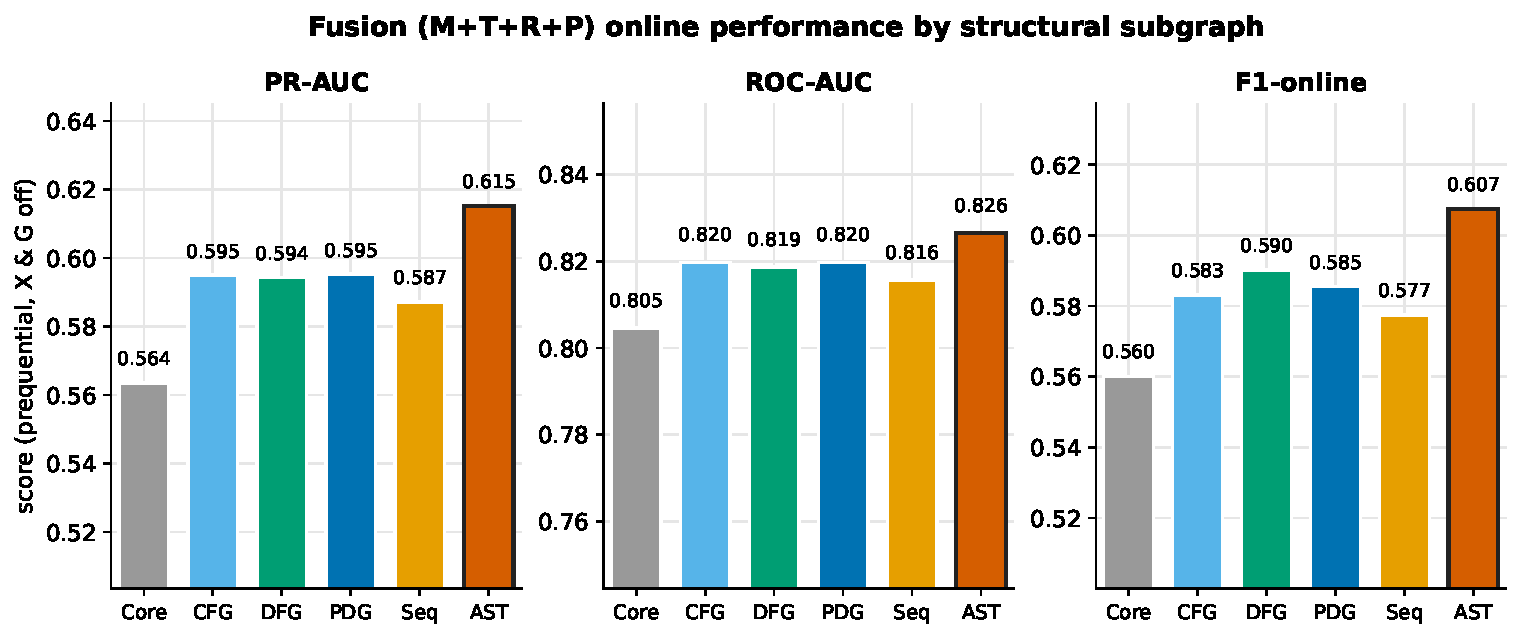
\includegraphics[width=\linewidth]{v4/fig_fusion_metrics}
		\caption{Fusion ($M{+}T{+}R{+}P$) online performance by structural subgraph
		(X and G off). AST is highest on PR-AUC, ROC-AUC and online-F1.}
		\label{fig:v4-fusion}
	\end{figure}

	\begin{figure}[t]
		\centering
		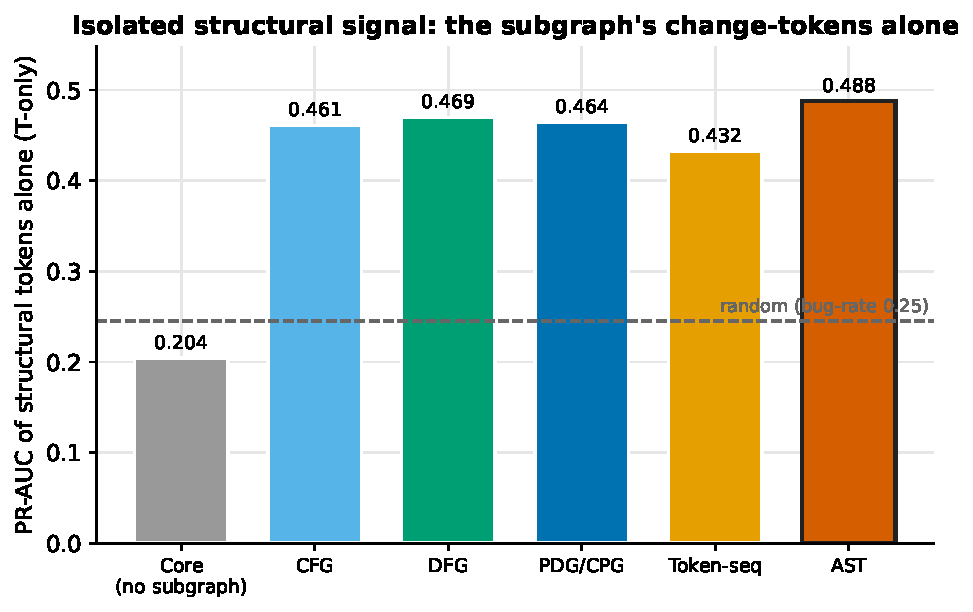
\includegraphics[width=.70\linewidth]{v4/fig_tonly_signal}
		\caption{Isolated structural signal: PR-AUC of each subgraph's change-tokens
		alone ($T$-only). The dashed line is the random (stream bug-rate) baseline.}
		\label{fig:v4-signal}
	\end{figure}

	\begin{figure}[t]
		\centering
		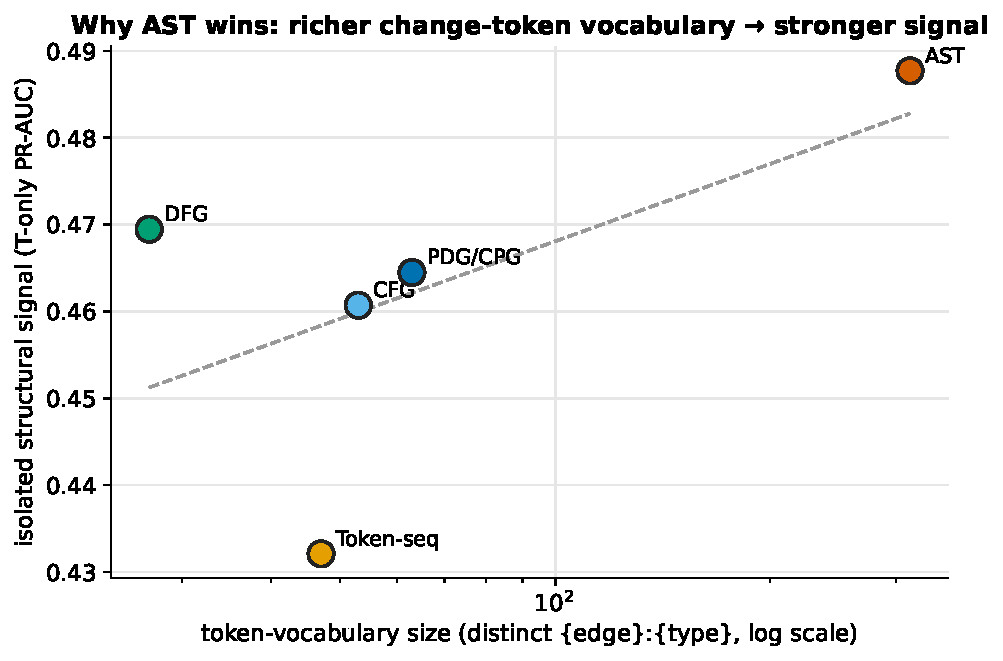
\includegraphics[width=.70\linewidth]{v4/fig_vocab_scatter}
		\caption{Why AST wins: richer change-token vocabulary yields a stronger
		isolated structural signal. AST sits top-right (both richest vocabulary and
		strongest signal); the weak token-sequence falls below the trend.}
		\label{fig:v4-vocab}
	\end{figure}

	\begin{figure}[t]
		\centering
		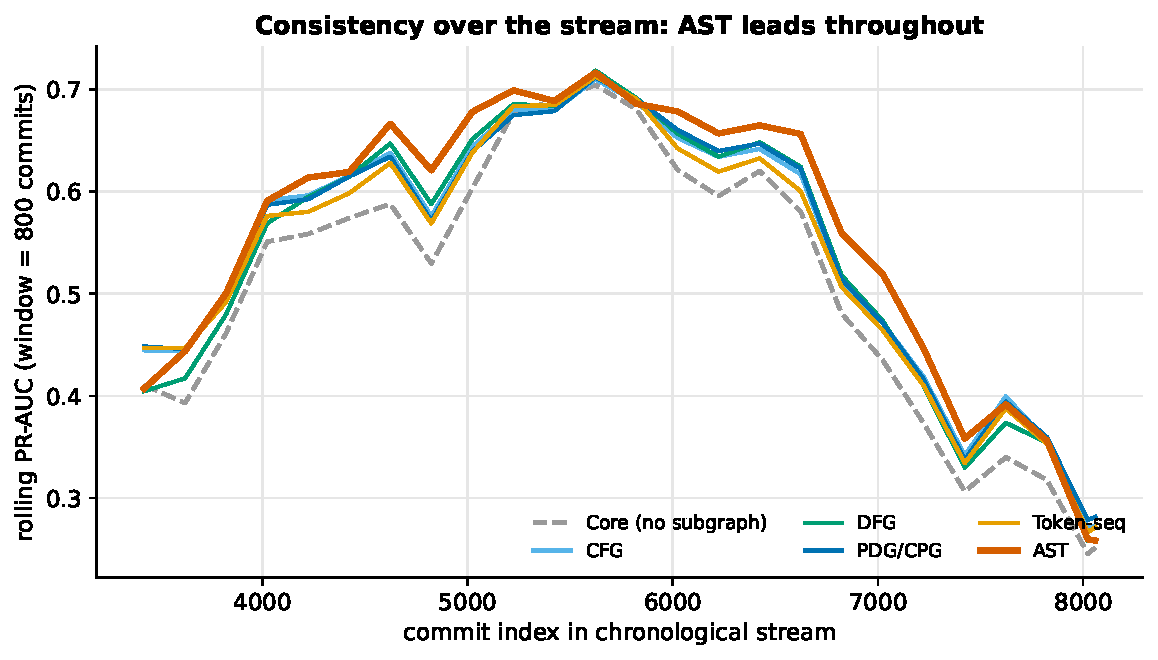
\includegraphics[width=\linewidth]{v4/fig_trajectory}
		\caption{Rolling PR-AUC (window $=800$ commits) over the chronological
		stream. AST (bold) leads throughout; core (dashed) trails throughout.}
		\label{fig:v4-traj}
	\end{figure}

	\subsection{The seven headline metrics}\label{sec:v4-metrics}
	Because the buggy class is the minority, threshold-free ranking scores alone can
	flatter a model. We therefore report the project's seven headline metrics ---
	\textbf{Precision}, \textbf{Recall}, \textbf{Macro-F1}, \textbf{Buggy-F1},
	\textbf{G-Mean}, \textbf{AUC} and \textbf{Accuracy}. The threshold-based metrics
	are taken at the leakage-free \emph{online-tuned} operating point (the decision
	threshold is retuned prequentially on past predictions only, maximising buggy-F1;
	\code{online\_jit.online\_decisions}); AUC is threshold-free.

	\paragraph{Definitions.} With true/false positives/negatives
	$\mathrm{TP},\mathrm{FP},\mathrm{TN},\mathrm{FN}$ for the buggy (positive) class:
	$\mathrm{Precision}=\tfrac{\mathrm{TP}}{\mathrm{TP}+\mathrm{FP}}$,
	$\mathrm{Recall}=\tfrac{\mathrm{TP}}{\mathrm{TP}+\mathrm{FN}}$ (buggy sensitivity),
	and \textbf{Buggy-F1} their harmonic mean
	$\tfrac{2\,\mathrm{Prec}\cdot\mathrm{Rec}}{\mathrm{Prec}+\mathrm{Rec}}$.
	\textbf{Macro-F1} averages the F1 of the buggy and the benign class (so both
	classes count equally under imbalance). \textbf{G-Mean}
	$=\sqrt{\mathrm{Recall}\cdot\mathrm{Specificity}}$ with
	$\mathrm{Specificity}=\tfrac{\mathrm{TN}}{\mathrm{TN}+\mathrm{FP}}$ rewards
	balanced performance on both classes. \textbf{AUC} is the area under the ROC curve
	(threshold-free ranking quality), and \textbf{Accuracy} the overall correct rate.
	Precision, Recall, the two F1s, G-Mean and Accuracy are computed from the
	online-tuned hard decisions; AUC from the raw scores.
	Table~\ref{tab:v4-metrics-fusion} and Figure~\ref{fig:v4-metrics-fusion} give the
	deployed Fusion model across subgraphs: \textbf{AST is best on all seven metrics}.

	\begin{table}[t]
	\centering
	\caption{Deployed Fusion ($M{+}T{+}R{+}P$) model across structural subgraphs on
	the seven headline metrics (Groovy; X and G off; threshold-based metrics at the
	online-tuned operating point). Best per column in \textbf{bold}.}
	\label{tab:v4-metrics-fusion}
	\begin{tabular}{lrrrrrrr}
	\toprule
	Subgraph & Prec. & Rec. & Macro-F1 & Buggy-F1 & G-Mean & AUC & Acc. \\
	\midrule
	Core & 0.467 & 0.700 & 0.683 & 0.560 & 0.720 & 0.805 & 0.731 \\
	\midrule
	CFG & 0.488 & 0.724 & 0.700 & 0.583 & 0.739 & 0.820 & 0.746 \\
	DFG & 0.495 & 0.730 & 0.706 & 0.590 & 0.744 & 0.819 & 0.752 \\
	PDG & 0.488 & 0.732 & 0.701 & 0.585 & 0.741 & 0.820 & 0.746 \\
	Seq & 0.493 & 0.697 & 0.700 & 0.577 & 0.731 & 0.816 & 0.750 \\
	AST & \textbf{0.510} & \textbf{0.750} & \textbf{0.719} & \textbf{0.607} & \textbf{0.758} & \textbf{0.826} & \textbf{0.762} \\
	\bottomrule
	\end{tabular}
	\end{table}

	\begin{figure}[t]
		\centering
		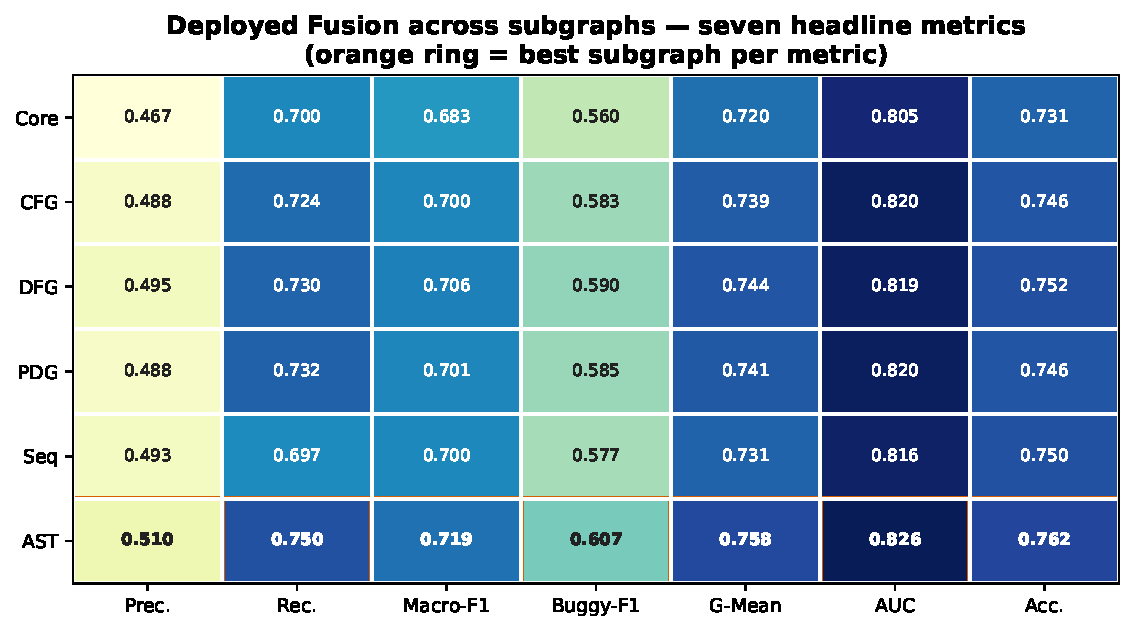
\includegraphics[width=\linewidth]{v4/fig_metrics_fusion}
		\caption{Deployed Fusion across subgraphs on the seven headline metrics; the
		best subgraph per metric is ringed. AST wins every column.}
		\label{fig:v4-metrics-fusion}
	\end{figure}

	\subsection{Per-method comparison: it is not only Fusion}\label{sec:v4-permethod}
	The Fusion result answers the deployment question, but a thorough analysis
	should ask whether \emph{each} inference method individually prefers the AST
	subgraph. We therefore run the full method suite of Section~\ref{sec:onlinejit}
	\emph{separately} on every layer. Two methods are \textbf{subgraph-independent
	references} --- JIT metrics~($M$, logistic regression) and relational
	priors~($R$, wvRN) --- because they never consume the structural tokens; four
	are \textbf{subgraph-dependent}: structural TF--IDF~($T$), Personalized
	PageRank~($P$), the SVD/LSA \emph{KG embedding}~($E$) of the commit--hub
	incidence matrix, and Fusion. Table~\ref{tab:v4-permethod} and
	Figure~\ref{fig:v4-heatmap} give the full $\text{method}\times\text{subgraph}$
	grid.

	\begin{table}[t]
	\centering
	\caption{Per-method online PR-AUC under each structural subgraph (Groovy; X and
	G off). Rows marked $^\star$ consume the subgraph's change-tokens and therefore
	vary; JIT-metrics and relational-priors are subgraph-independent references.
	Best structural variant per row in \textbf{bold}.}
	\label{tab:v4-permethod}
	\begin{tabular}{lrrrrrr}
	\toprule
	Method & Core & CFG & DFG & PDG & Seq & AST \\
	\midrule
	JIT metrics & 0.398 & 0.398 & 0.398 & 0.398 & 0.398 & 0.398 \\
	Relational priors & 0.460 & 0.460 & 0.460 & 0.460 & 0.460 & 0.460 \\
	\midrule
	Structural TF-IDF$^\star$ & 0.204 & 0.461 & 0.469 & 0.464 & 0.432 & \textbf{0.488} \\
	Personalized PageRank$^\star$ & \textbf{0.439} & 0.379 & 0.367 & 0.378 & 0.377 & 0.361 \\
	KG embedding (SVD)$^\star$ & 0.402 & 0.469 & \textbf{0.494} & 0.461 & 0.450 & 0.421 \\
	Fusion ($M{+}T{+}R{+}P$)$^\star$ & 0.564 & 0.595 & 0.594 & 0.595 & 0.587 & \textbf{0.615} \\
	\bottomrule
	\end{tabular}
	\end{table}

	\begin{figure}[t]
		\centering
		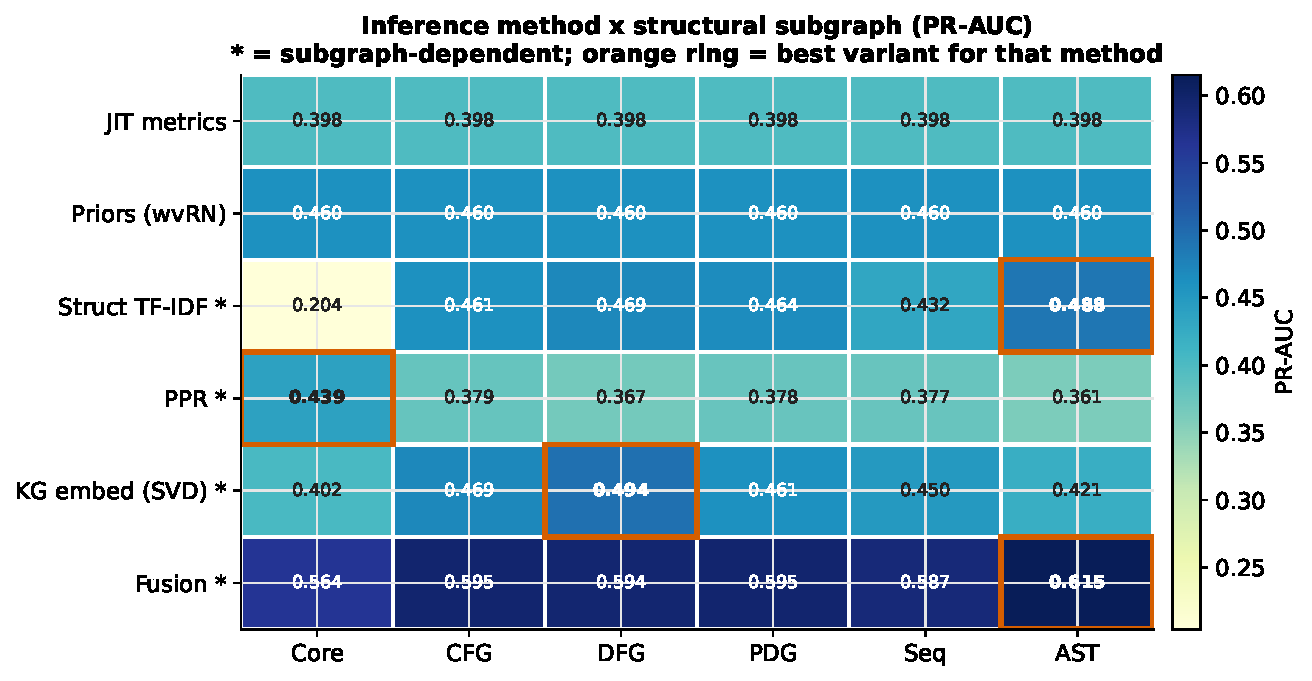
\includegraphics[width=\linewidth]{v4/fig_permethod_heatmap}
		\caption{PR-AUC of every inference method (rows) under every structural
		subgraph (columns). The two references ($M$, $R$) are flat by construction;
		for each subgraph-dependent method ($^\star$) the best variant is ringed.}
		\label{fig:v4-heatmap}
	\end{figure}

	\paragraph{Findings.} The picture is more nuanced --- and more honest --- than a
	uniform ``AST wins everywhere'':
	\begin{itemize}[nosep,leftmargin=1.4em]
		\item The references are \textbf{flat} across subgraphs ($M=0.398$,
		$R=0.460$ PR-AUC), a sanity check that they carry no structural information.
		\item \textbf{Structural TF--IDF} --- the most direct use of the
		change-tokens --- is \textbf{best with AST} ($0.488$), the cleanest
		expression of AST's advantage.
		\item \textbf{PPR} is \emph{best with no subgraph} (Core $0.439$): injecting
		typed token hubs dilutes the file/developer relational random walk rather
		than helping it --- PPR's signal is relational, not structural.
		\item The \textbf{KG embedding} is \emph{best with DFG} ($0.494$, above AST's
		$0.421$): AST's large, sparse $314$-type token vocabulary is harder to
		compress into a low-rank embedding than DFG's compact $27$-type one.
		\item \textbf{Fusion} --- the model we deploy --- is \textbf{best with AST}
		($0.615$), because it exploits AST's strong direct-token signal while the
		other channels contribute their subgraph-independent parts.
	\end{itemize}
	AST's superiority is thus \emph{method-specific}: it dominates the direct
	change-token channel~($T$) and the combined Fusion, which is precisely the
	basis on which the structural layer is chosen. The remaining nuances (PPR
	favouring the relational core, the embedding favouring the compact DFG) are
	reported rather than hidden, and do not change the deployment conclusion.

	\subsection{Five new graph-native online KG-inference methods}\label{sec:v4-graphnative}
	\paragraph{Motivation.} The methods above mix graph and non-graph evidence: $M$
	is purely tabular JIT metrics, $R$ blends relational rates with temporal priors,
	and Fusion welds them together. To measure the graph itself we add \textbf{five
	typical, purely graph-native, online KG-inference methods}, each consuming only
	the commit--hub graph and only strictly-past labels/edges
	(\code{inference/kg\_methods.py}). These are \emph{additive} --- the original
	methods and their results are retained.

	\paragraph{Graph and notation.} All five operate on the bipartite
	\emph{commit--hub} network $G=(\mathcal{C}\cup\mathcal{H},\,\mathcal{E})$, where
	$\mathcal{C}$ are commit nodes and $\mathcal{H}$ are hub nodes (change-tokens,
	and --- in the full scope --- files and developers). An edge $(c,h)$ means commit
	$c$ touches hub $h$; let $\mathbf{B}\in\mathbb{R}^{|\mathcal{C}|\times|\mathcal{H}|}$
	be the TF--IDF-weighted incidence matrix ($\mathbf{b}_c$ its row for commit $c$),
	$\mathcal{H}(c)$ the hubs of $c$, and $\mathcal{C}(h)$ the commits of $h$. Every
	method predicts commit $c$ from \emph{strictly past} commits
	$\mathrm{past}(c)=\{c':t_{c'}<t_c\}$ and their known labels $y\in\{0,1\}$ (buggy),
	so nothing at or after $c$ is used --- the leakage-free prequential protocol of
	Section~\ref{sec:onlinejit}.

	\paragraph{RN --- weighted-vote relational neighbour.} A collective-classification
	classifier (the wvRN of Macskassy \& Provost): a commit inherits the labels of
	past commits with which it shares hubs, weighted by the strength of the overlap,
	\[
	  s_{\mathrm{RN}}(c)=\frac{\sum_{c'\in\mathrm{past}(c)}\langle\mathbf{b}_c,\mathbf{b}_{c'}\rangle\,y_{c'}}
	                          {\sum_{c'\in\mathrm{past}(c)}\langle\mathbf{b}_c,\mathbf{b}_{c'}\rangle},
	\]
	i.e.\ the TF--IDF-weighted buggy-rate of $c$'s two-hop neighbourhood through
	shared hubs. No training; purely a function of the graph and past labels.

	\paragraph{PPR --- class-seeded Personalized PageRank.} A random-walk-with-restart
	over $G$. With column-normalised symmetric transition $\mathbf{P}$ and a restart
	distribution $\mathbf{s}$ concentrated on the past \emph{buggy} seeds, the
	stationary vector solves $\mathbf{r}^{+}=(1-\alpha)\mathbf{P}\mathbf{r}^{+}+\alpha\mathbf{s}^{+}$
	(power iteration); $\mathbf{r}^{-}$ is the analogue for the \emph{benign} seeds.
	The score is the relative buggy affinity
	$s_{\mathrm{PPR}}(c)=r^{+}(c)/\!\left(r^{+}(c)+r^{-}(c)\right)$. Seeds are past-only,
	so the walk never sees a future label.

	\paragraph{LP --- label propagation.} Spreading activation of known labels through
	the graph: initialise $f^{(0)}$ with the past labels (unknowns at the prior bug
	rate) and iterate a commit$\to$hub$\to$commit diffusion,
	$f^{(t+1)}=\widehat{\mathbf{B}}\,\widehat{\mathbf{B}}^{\!\top}f^{(t)}$ with
	row-normalised $\widehat{\mathbf{B}}$, re-clamping the past labels after each of a
	few steps; the score is the settled activation $f(c)$. It differs from PPR in
	propagating \emph{labels} rather than restart mass.

	\paragraph{DW --- DeepWalk embedding.} A random-walk graph embedding in its
	matrix-factorisation (Levy--Goldberg / NetMF) form: form the positive pointwise
	mutual information of the commit--hub co-occurrence,
	$\mathrm{PPMI}(c,h)=\max\!\big(\log\frac{x_{ch}\,\mathrm{vol}}{d_c\,d_h},\,0\big)$,
	and take a truncated SVD $\mathbf{U}\boldsymbol{\Sigma}\mathbf{V}^{\!\top}$; commit
	embeddings are $\mathbf{U}\boldsymbol{\Sigma}^{1/2}$. The PMI marginals and the SVD
	basis are fit on \emph{past} rows only, then all commits are projected; a logistic
	head trained on past embeddings produces the score. This replaces the earlier raw
	SVD ($E$) with a proper random-walk embedding.

	\paragraph{KGE --- DistMult knowledge-graph embedding.} A bilinear KG embedding
	over typed triples $(c,\rho,h)$ with relation $\rho\in\{\textsc{token},
	\textsc{file},\textsc{dev}\}$, scoring an edge by
	$\phi(c,\rho,h)=\sum_k e_c[k]\,w_\rho[k]\,e_h[k]=\langle\mathbf{e}_c,\mathbf{w}_\rho,\mathbf{e}_h\rangle$.
	Hub and relation embeddings are trained on the past triples by a logistic loss
	with negative (corrupted-tail) sampling; a commit --- including an unseen one at
	arrival --- is then \emph{folded in} as the mean of its incident
	$\mathbf{w}_\rho\!\odot\!\mathbf{e}_h$, and a logistic head on that embedding gives
	the score. Small dimension, few epochs, periodic refit on the growing past keep it
	CPU-cheap.

	\paragraph{Two graph scopes.} To avoid confounding the structural subgraph with
	the shared relational layer, each method is run on two scopes: \textbf{subgraph}
	(commits linked only to their change-token hubs --- the graph the subgraph
	actually defines) and \textbf{full} (token \emph{plus} file and developer hubs
	--- the deployed heterogeneous graph). Table~\ref{tab:v4-metrics-allmethods}
	lists every method on all seven metrics at the AST subgraph;
	Table~\ref{tab:v4-metrics-kgbf1} and Figure~\ref{fig:v4-kgbf1} give the
	graph-native methods across subgraphs.

	\begin{table}[t]
	\centering
	\caption{All inference methods on the AST subgraph, seven headline metrics:
	original methods, then the five graph-native methods on the subgraph-only and
	full scopes. Best per column in \textbf{bold}.}
	\label{tab:v4-metrics-allmethods}
	\small
	\begin{tabular}{lrrrrrrr}
	\toprule
	Method & Prec. & Rec. & Macro-F1 & Buggy-F1 & G-Mean & AUC & Acc. \\
	\midrule
	JIT metrics (M)            & 0.303 & 0.840 & 0.484 & 0.445 & 0.559 & 0.679 & 0.487 \\
	Relational priors (R)      & 0.360 & 0.809 & 0.583 & 0.498 & 0.656 & 0.733 & 0.600 \\
	Structural TF-IDF (T)      & 0.402 & 0.727 & 0.632 & 0.518 & 0.687 & 0.751 & 0.668 \\
	Personalized PageRank (P)  & 0.361 & 0.819 & 0.584 & 0.501 & 0.658 & 0.707 & 0.600 \\
	KG embedding SVD (E)       & 0.365 & 0.739 & 0.594 & 0.489 & 0.657 & 0.692 & 0.621 \\
	Fusion ($M{+}T{+}R{+}P$)   & \textbf{0.510} & 0.750 & \textbf{0.719} & \textbf{0.607} & \textbf{0.758} & \textbf{0.826} & \textbf{0.762} \\
	\midrule
	\multicolumn{8}{l}{\emph{graph-native, scope = subgraph}} \\
	Relational neighbour (RN)  & 0.301 & \textbf{0.906} & 0.460 & 0.452 & 0.535 & 0.638 & 0.461 \\
	PageRank RWR (PPR)         & 0.312 & 0.859 & 0.498 & 0.458 & 0.575 & 0.632 & 0.501 \\
	Label propagation (LP)     & 0.289 & 0.900 & 0.432 & 0.437 & 0.502 & 0.592 & 0.432 \\
	DeepWalk embed (DW)        & 0.370 & 0.732 & 0.599 & 0.492 & 0.660 & 0.709 & 0.629 \\
	KG embed DistMult (KGE)    & 0.347 & 0.778 & 0.568 & 0.480 & 0.638 & 0.681 & 0.586 \\
	\midrule
	\multicolumn{8}{l}{\emph{graph-native, scope = full}} \\
	Relational neighbour (RN)  & 0.299 & 0.900 & 0.457 & 0.449 & 0.532 & 0.638 & 0.458 \\
	PageRank RWR (PPR)         & 0.361 & 0.819 & 0.584 & 0.501 & 0.658 & 0.707 & 0.600 \\
	Label propagation (LP)     & 0.302 & 0.884 & 0.471 & 0.451 & 0.547 & 0.642 & 0.472 \\
	DeepWalk embed (DW)        & 0.369 & 0.711 & 0.599 & 0.486 & 0.656 & 0.691 & 0.632 \\
	KG embed DistMult (KGE)    & 0.347 & 0.753 & 0.571 & 0.475 & 0.638 & 0.696 & 0.593 \\
	\bottomrule
	\end{tabular}
	\end{table}

	\begin{table}[t]
	\centering
	\caption{The five graph-native methods across structural subgraphs (Buggy-F1),
	on the subgraph-only and full graph scopes. Best subgraph per row in
	\textbf{bold}.}
	\label{tab:v4-metrics-kgbf1}
	\begin{tabular}{lrrrrrr}
	\toprule
	Method & Core & CFG & DFG & PDG & Seq & AST \\
	\midrule
	\multicolumn{7}{l}{\emph{scope: subgraph}} \\
	Relational neighbour (RN) & 0.393 & 0.452 & \textbf{0.459} & 0.450 & 0.447 & 0.452 \\
	PageRank RWR (PPR) & 0.393 & \textbf{0.466} & 0.464 & 0.458 & 0.462 & 0.458 \\
	Label propagation (LP) & 0.393 & 0.446 & \textbf{0.453} & 0.444 & 0.442 & 0.437 \\
	DeepWalk embed (DW) & 0.394 & 0.486 & 0.473 & 0.481 & 0.477 & \textbf{0.492} \\
	KG embed DistMult (KGE) & 0.394 & 0.476 & \textbf{0.482} & 0.472 & 0.475 & 0.480 \\
	\midrule
	\multicolumn{7}{l}{\emph{scope: full}} \\
	Relational neighbour (RN) & \textbf{0.493} & 0.451 & 0.457 & 0.449 & 0.449 & 0.449 \\
	PageRank RWR (PPR) & 0.499 & 0.501 & \textbf{0.508} & 0.498 & 0.502 & 0.501 \\
	Label propagation (LP) & 0.459 & 0.459 & \textbf{0.468} & 0.455 & 0.456 & 0.451 \\
	DeepWalk embed (DW) & 0.466 & 0.466 & 0.461 & 0.468 & 0.458 & \textbf{0.486} \\
	KG embed DistMult (KGE) & 0.426 & 0.470 & 0.459 & 0.461 & 0.457 & \textbf{0.475} \\
	\bottomrule
	\end{tabular}
	\end{table}

	\begin{figure}[t]
		\centering
		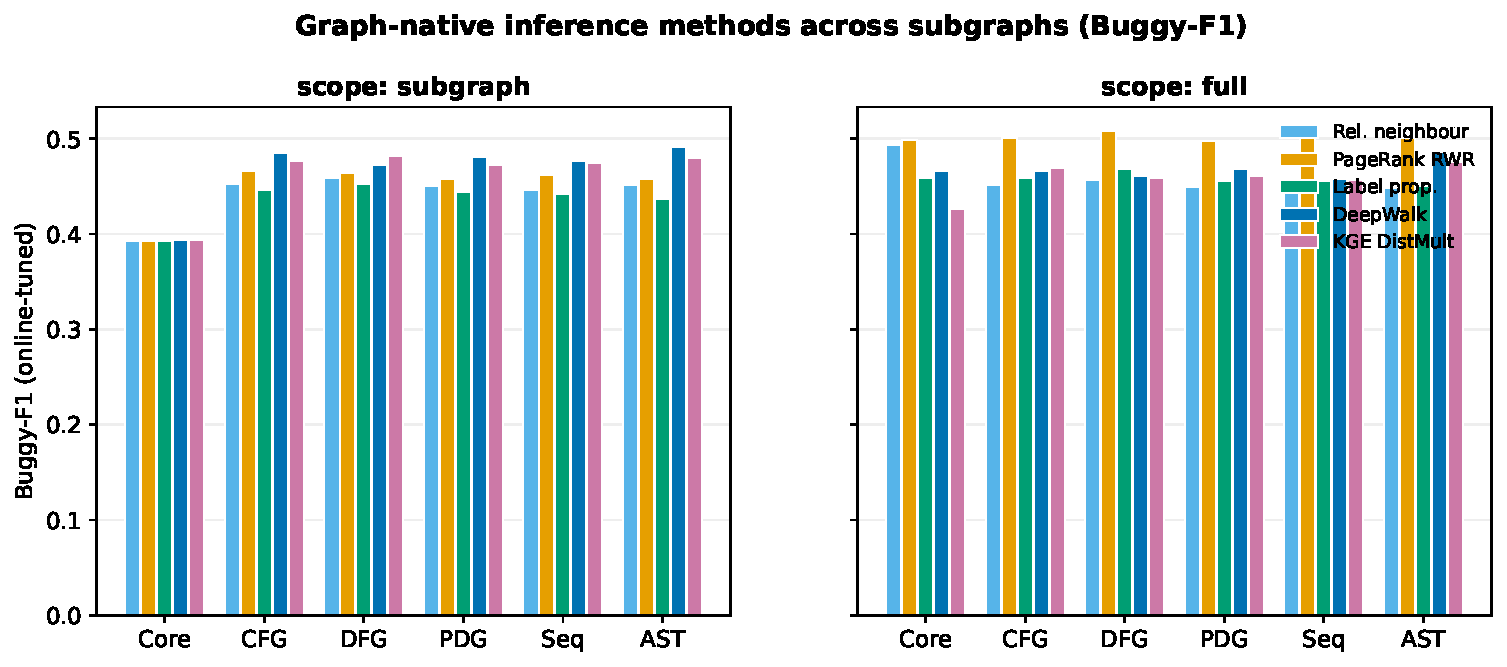
\includegraphics[width=\linewidth]{v4/fig_kg_methods_bf1}
		\caption{The five graph-native methods across subgraphs (Buggy-F1), on the
		subgraph-only (left) and full (right) scopes.}
		\label{fig:v4-kgbf1}
	\end{figure}

	\paragraph{Findings.} Two regimes emerge, cleanly separated by scope.
	\emph{Random-walk and propagation} methods (RN, PPR, LP) are strongest on the
	relational (core/full) graph and are \emph{diluted} by structural tokens --- their
	signal is relational (file/developer), not structural; the pure relational
	methods also reach very high Recall at the cost of Precision (they flag buggy
	liberally). The \emph{embedding} methods (DeepWalk, KGE) instead prefer the
	token-rich subgraphs and rank \textbf{AST} highest among them, echoing the
	structural TF-IDF result. On the AST subgraph the deployed \textbf{Fusion still
	dominates the balanced metrics} (Macro-F1, Buggy-F1, G-Mean, AUC, Accuracy;
	Table~\ref{tab:v4-metrics-allmethods}). Reporting both scopes removes the
	file/developer confound: the subgraph scope isolates \emph{what the subgraph
	adds}, and there the embedding methods again favour AST.

	\subsection{Choosing the final fusion formula}\label{sec:v4-fusionablation}
	The subgraph study fixes AST as the structural layer; we now choose the
	\emph{inference fusion} for the complete method (Core~$+$~AST~$+$~CSTG, still
	without commit text~$X$), with an explicit goal of a \textbf{purely graph-native}
	predictor. We ablate \textbf{all combinations} of ten inference methods on the
	final graph --- the previous $M,R,T,P,E,G$(CSTG) and the five new graph-native
	$RN,LP,DW,KGE$ --- under two fusion styles (\code{inference/run\_fusion\_ablation.py}):
	\emph{score stacking} (a prequential logistic regression over the selected
	methods' probabilities; all $2^{10}-1=1023$ subsets) and \emph{feature fusion}
	(concatenated raw feature blocks of the top channels; all $2^{6}-1=63$ subsets).
	Every subset is scored on all seven headline metrics.

	\paragraph{Single channels.} Table~\ref{tab:v4-fusion-singles} ranks the ten
	methods individually. Two facts drive the choice: the \textbf{CSTG semantic-text
	channel $G$ is by far the strongest single signal} (Buggy-F1 $0.596$), and the
	\textbf{non-graph JIT metrics $M$ are among the \emph{weakest}} (Buggy-F1
	$0.476$) --- so dropping $M$ costs almost nothing.

	\begin{table}[t]
	\centering \small
	\caption{Single inference methods on the final graph (Core+AST+CSTG, no X), seven
	headline metrics, ranked by Buggy-F1. CSTG ($G$) is the strongest single channel;
	the non-graph JIT metrics ($M$) are near the weakest.}
	\label{tab:v4-fusion-singles}
	\resizebox{\textwidth}{!}{%
	\begin{tabular}{lccrrrrrrr}
	\toprule
	Method & graph & \#ch & Prec. & Rec. & Macro-F1 & Buggy-F1 & G-Mean & AUC & Acc. \\
	\midrule
	G   & \checkmark & 1 & 0.517 & 0.702 & 0.716 & 0.596 & 0.743 & 0.824 & 0.766 \\
	T   & \checkmark & 1 & 0.418 & 0.710 & 0.646 & 0.526 & 0.694 & 0.759 & 0.687 \\
	P   & \checkmark & 1 & 0.374 & 0.815 & 0.600 & 0.512 & 0.673 & 0.720 & 0.619 \\
	R   & \checkmark & 1 & 0.388 & 0.752 & 0.618 & 0.512 & 0.680 & 0.746 & 0.648 \\
	KGE & \checkmark & 1 & 0.381 & 0.754 & 0.611 & 0.506 & 0.674 & 0.727 & 0.639 \\
	DW  & \checkmark & 1 & 0.401 & 0.664 & 0.629 & 0.500 & 0.671 & 0.716 & 0.674 \\
	LP  & \checkmark & 1 & 0.340 & 0.914 & 0.540 & 0.496 & 0.623 & 0.711 & 0.545 \\
	E   & \checkmark & 1 & 0.425 & 0.579 & 0.641 & 0.490 & 0.657 & 0.716 & 0.705 \\
	M   & --         & 1 & 0.346 & 0.765 & 0.568 & 0.476 & 0.636 & 0.701 & 0.587 \\
	RN  & \checkmark & 1 & 0.317 & 0.901 & 0.498 & 0.469 & 0.577 & 0.652 & 0.500 \\
	\bottomrule
	\end{tabular}%
	}
	\end{table}

	\paragraph{Combined fusions and the final choice.}
	Table~\ref{tab:v4-fusion-recommend} and Figure~\ref{fig:v4-pareto} summarise the
	combinations. Performance saturates at three to four components; adding further
	methods (up to a seven-method graph-only stack, Buggy-F1 $0.618$) yields only
	marginal gains. We therefore adopt the compact, purely graph-native
	\textbf{Fusion $=R+T+G$} (relational priors $+$ AST structural change-tokens $+$
	CSTG semantics). Relative to the previous metrics-inclusive $M{+}T{+}R{+}P$ it
	improves the minority-class metrics --- Recall $0.768$ ($+0.078$), Buggy-F1
	$0.608$ ($+0.016$), G-Mean $0.761$ ($+0.022$), AUC $0.834$ ($+0.014$), Macro-F1
	$0.716$ ($+0.002$) --- for small trades in Precision ($-0.015$) and Accuracy
	($-0.010$), i.e.\ a healthier recall-oriented operating point for the minority
	buggy class, while \textbf{dropping the non-graph JIT metrics} and using fewer
	channels.

	\begin{table}[t]
	\centering \small
	\caption{Candidate final Fusion formulas on the seven headline metrics
	(feature-fusion unless noted; online-tuned operating point). The recommended
	purely graph-native \textbf{R+T+G} improves on the previous metrics-inclusive
	$M{+}T{+}R{+}P$ on the minority-class metrics (Recall, Buggy-F1, G-Mean, AUC,
	Macro-F1) while dropping the non-graph JIT metrics and using fewer channels.}
	\label{tab:v4-fusion-recommend}
	\resizebox{\textwidth}{!}{%
	\begin{tabular}{lccrrrrrrr}
	\toprule
	Fusion & graph & \#ch & Prec. & Rec. & Macro-F1 & Buggy-F1 & G-Mean & AUC & Acc. \\
	\midrule
	M+T+R+P (previous Fusion)              & --         & 4 & 0.519 & 0.690 & 0.715 & 0.593 & 0.739 & 0.820 & 0.767 \\
	M+R+T+G (best overall)                 & --         & 4 & 0.541 & 0.727 & 0.734 & 0.620 & 0.762 & 0.832 & 0.782 \\
	R+T+P+G+RN+LP+KGE (best graph stack)   & \checkmark & 7 & 0.549 & 0.708 & 0.735 & 0.618 & 0.758 & 0.843 & 0.786 \\
	\midrule
	R+T+P+G                                & \checkmark & 4 & 0.506 & 0.745 & 0.715 & 0.603 & 0.755 & 0.834 & 0.759 \\
	T+G (structure+semantics)              & \checkmark & 2 & 0.495 & 0.768 & 0.711 & 0.602 & 0.757 & 0.827 & 0.751 \\
	\textbf{R+T+G (recommended)}           & \checkmark & 3 & 0.504 & 0.768 & 0.716 & 0.608 & 0.761 & 0.834 & 0.758 \\
	\bottomrule
	\end{tabular}%
	}
	\end{table}

	\begin{figure}[t]
		\centering
		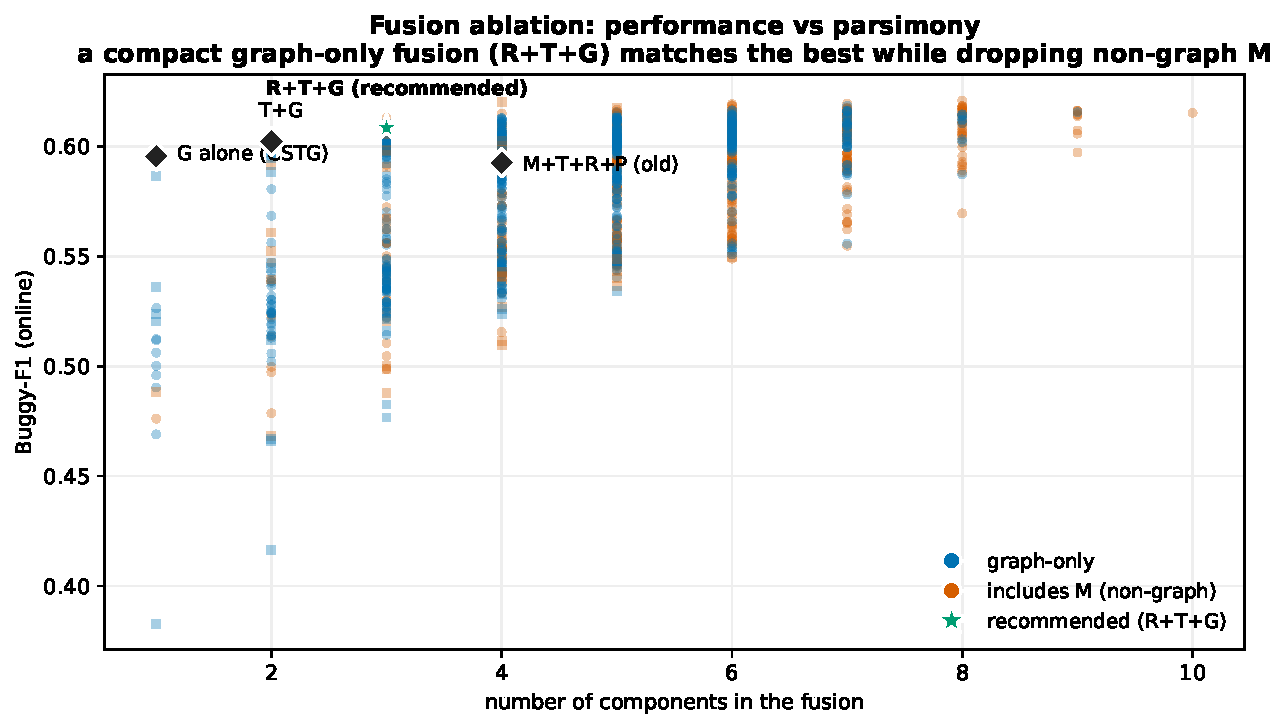
\includegraphics[width=.85\linewidth]{v4/fig_fusion_pareto}
		\caption{Fusion ablation --- Buggy-F1 versus number of components. Blue =
		graph-only, orange = includes the non-graph $M$. Performance saturates by
		three to four components; the recommended graph-only \textbf{R+T+G} (green
		star) sits near the top of the cloud with only three channels.}
		\label{fig:v4-pareto}
	\end{figure}

	\subsection{Full ablation: the best fusions at every size}\label{sec:v4-bysize}
	The complete ablation evaluates all $2^{10}-1=1023$ score-stacking combinations;
	reporting every row is impractical, so Tables~\ref{tab:v4-fusion-k1}--\ref{tab:v4-fusion-k10}
	give, for each fusion size $k=1,\dots,10$, the \textbf{best eight $k$-method
	fusions} by Buggy-F1 (the last has a single $10$-method combination), on all seven
	metrics. Two aggregate views summarise the $1023$ points:
	Figure~\ref{fig:v4-bysize} shows the Buggy-F1 distribution at each size with the
	best-per-size envelope, and Figure~\ref{fig:v4-methodfreq} shows how often each
	method appears among the very best fusions.

	\paragraph{Reading the tables.} Three patterns recur. (i)~\textbf{Performance
	saturates early}: the best fusion already reaches Buggy-F1~$\approx0.61$ at
	$k=3$ and only inches to $0.621$ by $k=8$, so large fusions are not worth their
	complexity. (ii)~\textbf{$R$, $T$ and $G$ are near-universal} in the top fusions
	at every size (Figure~\ref{fig:v4-methodfreq}), confirming them as the essential
	trio. (iii)~\textbf{Graph-only fusions track the metrics-inclusive ones closely}
	at every size --- e.g.\ at $k=3$ the graph-only $R{+}T{+}G$ ($0.610$) trails the
	$M$-containing $M{+}R{+}G$ ($0.613$) by only $0.003$ --- so dropping the non-graph
	$M$ costs almost nothing, which is exactly why the compact graph-only
	$R{+}T{+}G$ is adopted.

	\begin{figure}[H]
		\centering
		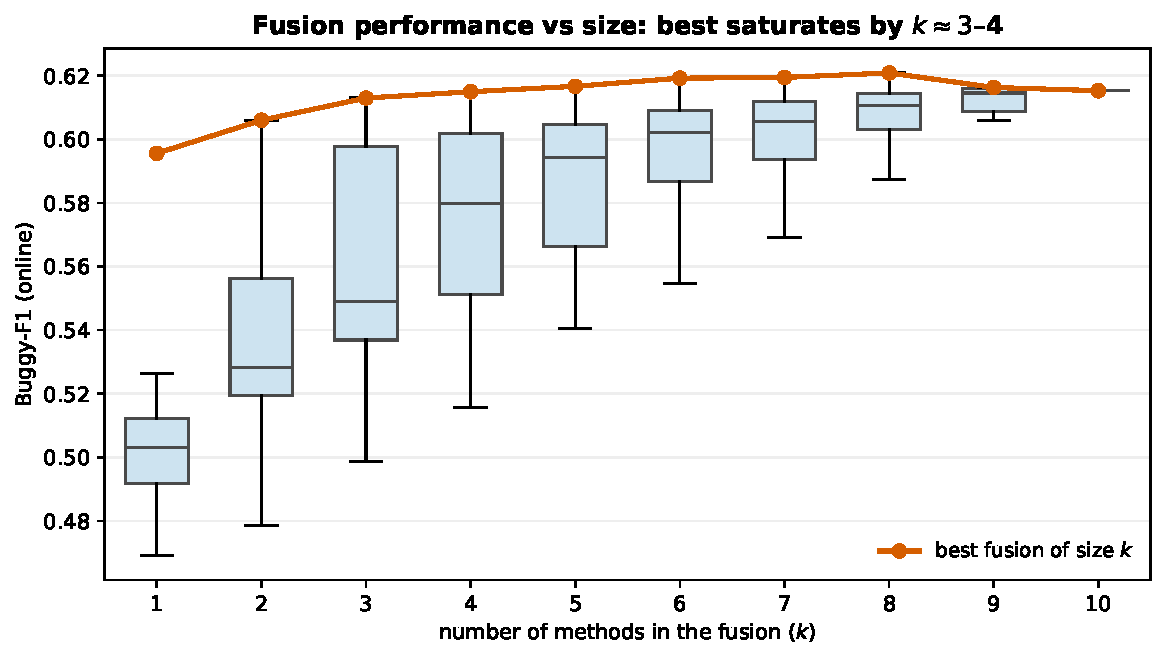
\includegraphics[width=.85\linewidth]{v4/fig_ablation_bysize}
		\caption{Buggy-F1 of all fusions at each size $k$ (boxes) with the
		best-per-size envelope (orange). The best value saturates by $k\approx3$--4.}
		\label{fig:v4-bysize}
	\end{figure}

	\begin{figure}[H]
		\centering
		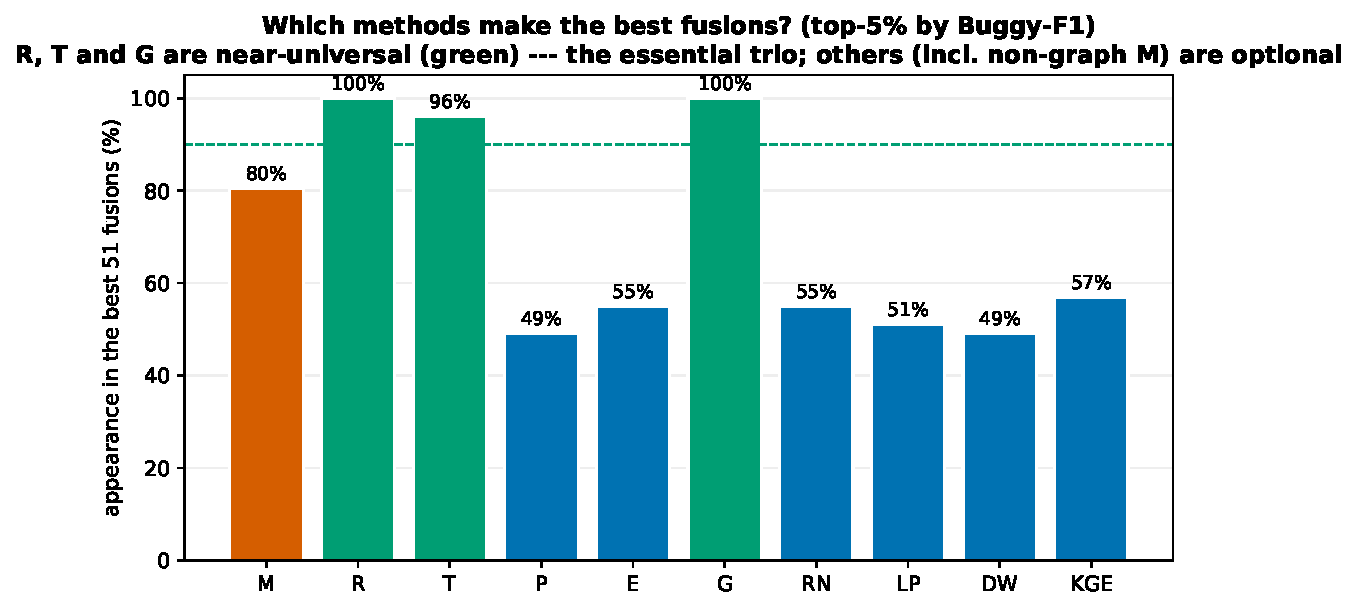
\includegraphics[width=.80\linewidth]{v4/fig_ablation_method_freq}
		\caption{How often each method appears in the best 5\% of fusions (by
		Buggy-F1). $R$, $T$ and $G$ (green) are near-universal --- the essential trio;
		the remaining methods, including the non-graph $M$, are optional.}
		\label{fig:v4-methodfreq}
	\end{figure}

	\begin{table}[H]
\centering \scriptsize
\caption{Best 8 fusion(s) of $k=1$ method by Buggy-F1 (score-stacking over the ten inference methods; final Core+AST+CSTG graph, no X). ``graph'' = purely graph-native (no non-graph JIT metrics $M$).}
\label{tab:v4-fusion-k1}
\begin{tabular}{lcrrrrrrr}
\toprule
Fusion & graph & Prec. & Rec. & Macro-F1 & Buggy-F1 & G-Mean & AUC & Acc. \\
\midrule
G & \checkmark & 0.517 & 0.702 & 0.716 & 0.596 & 0.743 & 0.824 & 0.766 \\
T & \checkmark & 0.418 & 0.710 & 0.646 & 0.526 & 0.694 & 0.759 & 0.687 \\
P & \checkmark & 0.374 & 0.815 & 0.600 & 0.512 & 0.673 & 0.720 & 0.619 \\
R & \checkmark & 0.388 & 0.752 & 0.618 & 0.512 & 0.680 & 0.746 & 0.648 \\
KGE & \checkmark & 0.381 & 0.754 & 0.611 & 0.506 & 0.674 & 0.727 & 0.639 \\
DW & \checkmark & 0.401 & 0.664 & 0.629 & 0.500 & 0.671 & 0.716 & 0.674 \\
LP & \checkmark & 0.340 & 0.914 & 0.540 & 0.496 & 0.623 & 0.711 & 0.545 \\
E & \checkmark & 0.425 & 0.579 & 0.641 & 0.490 & 0.657 & 0.716 & 0.705 \\
\bottomrule
\end{tabular}
\end{table}

\begin{table}[H]
\centering \scriptsize
\caption{Best 8 fusion(s) of $k=2$ methods by Buggy-F1 (score-stacking over the ten inference methods; final Core+AST+CSTG graph, no X). ``graph'' = purely graph-native (no non-graph JIT metrics $M$).}
\label{tab:v4-fusion-k2}
\begin{tabular}{lcrrrrrrr}
\toprule
Fusion & graph & Prec. & Rec. & Macro-F1 & Buggy-F1 & G-Mean & AUC & Acc. \\
\midrule
R+G & \checkmark & 0.521 & 0.724 & 0.721 & 0.606 & 0.753 & 0.833 & 0.769 \\
G+KGE & \checkmark & 0.535 & 0.694 & 0.725 & 0.604 & 0.747 & 0.833 & 0.777 \\
T+G & \checkmark & 0.517 & 0.715 & 0.718 & 0.600 & 0.748 & 0.834 & 0.766 \\
P+G & \checkmark & 0.509 & 0.731 & 0.715 & 0.600 & 0.751 & 0.829 & 0.761 \\
G+LP & \checkmark & 0.521 & 0.707 & 0.719 & 0.600 & 0.747 & 0.828 & 0.769 \\
M+G & -- & 0.509 & 0.725 & 0.714 & 0.598 & 0.749 & 0.826 & 0.761 \\
G+DW & \checkmark & 0.515 & 0.713 & 0.716 & 0.598 & 0.747 & 0.828 & 0.765 \\
G+RN & \checkmark & 0.520 & 0.701 & 0.717 & 0.597 & 0.744 & 0.827 & 0.768 \\
\bottomrule
\end{tabular}
\end{table}

\begin{table}[H]
\centering \scriptsize
\caption{Best 8 fusion(s) of $k=3$ methods by Buggy-F1 (score-stacking over the ten inference methods; final Core+AST+CSTG graph, no X). ``graph'' = purely graph-native (no non-graph JIT metrics $M$).}
\label{tab:v4-fusion-k3}
\begin{tabular}{lcrrrrrrr}
\toprule
Fusion & graph & Prec. & Rec. & Macro-F1 & Buggy-F1 & G-Mean & AUC & Acc. \\
\midrule
M+R+G & -- & 0.512 & 0.764 & 0.721 & 0.613 & 0.764 & 0.836 & 0.763 \\
R+G+RN & \checkmark & 0.532 & 0.718 & 0.727 & 0.611 & 0.755 & 0.834 & 0.776 \\
R+G+KGE & \checkmark & 0.525 & 0.729 & 0.725 & 0.610 & 0.757 & 0.839 & 0.772 \\
R+T+G & \checkmark & 0.525 & 0.727 & 0.724 & 0.610 & 0.756 & 0.843 & 0.772 \\
P+G+KGE & \checkmark & 0.530 & 0.712 & 0.725 & 0.608 & 0.753 & 0.835 & 0.775 \\
R+G+LP & \checkmark & 0.518 & 0.734 & 0.721 & 0.608 & 0.756 & 0.834 & 0.768 \\
R+E+G & \checkmark & 0.531 & 0.711 & 0.725 & 0.608 & 0.752 & 0.837 & 0.775 \\
M+T+G & -- & 0.513 & 0.741 & 0.719 & 0.606 & 0.756 & 0.835 & 0.764 \\
\bottomrule
\end{tabular}
\end{table}

\begin{table}[H]
\centering \scriptsize
\caption{Best 8 fusion(s) of $k=4$ methods by Buggy-F1 (score-stacking over the ten inference methods; final Core+AST+CSTG graph, no X). ``graph'' = purely graph-native (no non-graph JIT metrics $M$).}
\label{tab:v4-fusion-k4}
\begin{tabular}{lcrrrrrrr}
\toprule
Fusion & graph & Prec. & Rec. & Macro-F1 & Buggy-F1 & G-Mean & AUC & Acc. \\
\midrule
M+R+T+G & -- & 0.518 & 0.756 & 0.724 & 0.615 & 0.764 & 0.845 & 0.768 \\
R+T+G+RN & \checkmark & 0.531 & 0.724 & 0.727 & 0.613 & 0.758 & 0.843 & 0.776 \\
R+T+G+DW & \checkmark & 0.519 & 0.747 & 0.724 & 0.613 & 0.761 & 0.843 & 0.768 \\
R+T+P+G & \checkmark & 0.530 & 0.726 & 0.727 & 0.612 & 0.758 & 0.843 & 0.775 \\
R+G+RN+KGE & \checkmark & 0.532 & 0.720 & 0.727 & 0.612 & 0.756 & 0.840 & 0.776 \\
R+T+G+KGE & \checkmark & 0.531 & 0.721 & 0.727 & 0.611 & 0.756 & 0.843 & 0.775 \\
R+G+RN+LP & \checkmark & 0.529 & 0.724 & 0.726 & 0.611 & 0.757 & 0.834 & 0.774 \\
M+R+G+RN & -- & 0.512 & 0.756 & 0.721 & 0.611 & 0.761 & 0.837 & 0.764 \\
\bottomrule
\end{tabular}
\end{table}

\begin{table}[H]
\centering \scriptsize
\caption{Best 8 fusion(s) of $k=5$ methods by Buggy-F1 (score-stacking over the ten inference methods; final Core+AST+CSTG graph, no X). ``graph'' = purely graph-native (no non-graph JIT metrics $M$).}
\label{tab:v4-fusion-k5}
\begin{tabular}{lcrrrrrrr}
\toprule
Fusion & graph & Prec. & Rec. & Macro-F1 & Buggy-F1 & G-Mean & AUC & Acc. \\
\midrule
M+R+T+G+DW & -- & 0.531 & 0.734 & 0.729 & 0.617 & 0.762 & 0.845 & 0.776 \\
M+R+T+G+RN & -- & 0.524 & 0.746 & 0.727 & 0.616 & 0.763 & 0.845 & 0.772 \\
R+T+G+RN+KGE & \checkmark & 0.539 & 0.717 & 0.731 & 0.616 & 0.758 & 0.843 & 0.780 \\
M+R+T+G+KGE & -- & 0.527 & 0.740 & 0.727 & 0.615 & 0.762 & 0.845 & 0.773 \\
M+R+T+E+G & -- & 0.522 & 0.750 & 0.726 & 0.615 & 0.763 & 0.845 & 0.770 \\
M+R+T+P+G & -- & 0.532 & 0.727 & 0.729 & 0.615 & 0.759 & 0.845 & 0.776 \\
M+R+T+G+LP & -- & 0.522 & 0.746 & 0.725 & 0.614 & 0.762 & 0.845 & 0.770 \\
R+G+RN+LP+KGE & \checkmark & 0.537 & 0.716 & 0.730 & 0.614 & 0.757 & 0.840 & 0.779 \\
\bottomrule
\end{tabular}
\end{table}

\begin{table}[H]
\centering \scriptsize
\caption{Best 8 fusion(s) of $k=6$ methods by Buggy-F1 (score-stacking over the ten inference methods; final Core+AST+CSTG graph, no X). ``graph'' = purely graph-native (no non-graph JIT metrics $M$).}
\label{tab:v4-fusion-k6}
\begin{tabular}{lcrrrrrrr}
\toprule
Fusion & graph & Prec. & Rec. & Macro-F1 & Buggy-F1 & G-Mean & AUC & Acc. \\
\midrule
M+R+T+G+RN+DW & -- & 0.529 & 0.747 & 0.730 & 0.619 & 0.765 & 0.845 & 0.775 \\
M+R+T+E+G+DW & -- & 0.529 & 0.744 & 0.730 & 0.619 & 0.764 & 0.844 & 0.775 \\
M+R+T+E+G+KGE & -- & 0.542 & 0.719 & 0.733 & 0.618 & 0.760 & 0.845 & 0.782 \\
M+R+T+G+RN+LP & -- & 0.527 & 0.744 & 0.728 & 0.617 & 0.763 & 0.845 & 0.774 \\
M+R+T+P+G+RN & -- & 0.533 & 0.731 & 0.730 & 0.617 & 0.761 & 0.845 & 0.777 \\
R+T+P+G+RN+KGE & \checkmark & 0.542 & 0.715 & 0.732 & 0.616 & 0.758 & 0.843 & 0.782 \\
R+T+G+RN+LP+KGE & \checkmark & 0.540 & 0.718 & 0.731 & 0.616 & 0.758 & 0.843 & 0.781 \\
M+R+T+G+LP+DW & -- & 0.529 & 0.736 & 0.728 & 0.616 & 0.761 & 0.845 & 0.775 \\
\bottomrule
\end{tabular}
\end{table}

\begin{table}[H]
\centering \scriptsize
\caption{Best 8 fusion(s) of $k=7$ methods by Buggy-F1 (score-stacking over the ten inference methods; final Core+AST+CSTG graph, no X). ``graph'' = purely graph-native (no non-graph JIT metrics $M$).}
\label{tab:v4-fusion-k7}
\begin{tabular}{lcrrrrrrr}
\toprule
Fusion & graph & Prec. & Rec. & Macro-F1 & Buggy-F1 & G-Mean & AUC & Acc. \\
\midrule
M+R+T+P+E+G+KGE & -- & 0.553 & 0.705 & 0.736 & 0.619 & 0.758 & 0.844 & 0.788 \\
R+T+P+G+RN+LP+KGE & \checkmark & 0.549 & 0.708 & 0.735 & 0.618 & 0.758 & 0.843 & 0.786 \\
M+R+T+G+RN+LP+DW & -- & 0.529 & 0.741 & 0.729 & 0.618 & 0.763 & 0.845 & 0.775 \\
M+R+T+P+G+LP+KGE & -- & 0.534 & 0.732 & 0.730 & 0.617 & 0.762 & 0.845 & 0.777 \\
M+R+T+P+G+RN+DW & -- & 0.542 & 0.717 & 0.732 & 0.617 & 0.759 & 0.845 & 0.782 \\
M+R+E+G+RN+LP+KGE & -- & 0.537 & 0.724 & 0.731 & 0.617 & 0.760 & 0.843 & 0.779 \\
M+R+T+P+G+RN+KGE & -- & 0.536 & 0.725 & 0.730 & 0.616 & 0.760 & 0.845 & 0.779 \\
R+T+P+G+LP+DW+KGE & \checkmark & 0.543 & 0.712 & 0.732 & 0.616 & 0.757 & 0.842 & 0.782 \\
\bottomrule
\end{tabular}
\end{table}

\begin{table}[H]
\centering \scriptsize
\caption{Best 8 fusion(s) of $k=8$ methods by Buggy-F1 (score-stacking over the ten inference methods; final Core+AST+CSTG graph, no X). ``graph'' = purely graph-native (no non-graph JIT metrics $M$).}
\label{tab:v4-fusion-k8}
\begin{tabular}{lcrrrrrrr}
\toprule
Fusion & graph & Prec. & Rec. & Macro-F1 & Buggy-F1 & G-Mean & AUC & Acc. \\
\midrule
M+R+T+P+G+RN+LP+DW & -- & 0.536 & 0.738 & 0.732 & 0.621 & 0.765 & 0.845 & 0.779 \\
M+R+T+P+E+G+RN+KGE & -- & 0.554 & 0.700 & 0.736 & 0.618 & 0.756 & 0.845 & 0.788 \\
M+R+T+P+E+G+LP+KGE & -- & 0.554 & 0.700 & 0.736 & 0.618 & 0.756 & 0.845 & 0.788 \\
M+R+T+P+E+G+LP+DW & -- & 0.542 & 0.718 & 0.733 & 0.618 & 0.759 & 0.844 & 0.782 \\
M+R+T+E+G+RN+LP+DW & -- & 0.535 & 0.731 & 0.731 & 0.618 & 0.762 & 0.844 & 0.778 \\
M+R+T+E+G+LP+DW+KGE & -- & 0.544 & 0.712 & 0.733 & 0.617 & 0.758 & 0.844 & 0.783 \\
M+R+T+E+G+RN+LP+KGE & -- & 0.542 & 0.715 & 0.732 & 0.617 & 0.758 & 0.845 & 0.782 \\
M+R+T+G+RN+LP+DW+KGE & -- & 0.536 & 0.726 & 0.730 & 0.617 & 0.760 & 0.845 & 0.779 \\
\bottomrule
\end{tabular}
\end{table}

\begin{table}[H]
\centering \scriptsize
\caption{Best 8 fusion(s) of $k=9$ methods by Buggy-F1 (score-stacking over the ten inference methods; final Core+AST+CSTG graph, no X). ``graph'' = purely graph-native (no non-graph JIT metrics $M$).}
\label{tab:v4-fusion-k9}
\begin{tabular}{lcrrrrrrr}
\toprule
Fusion & graph & Prec. & Rec. & Macro-F1 & Buggy-F1 & G-Mean & AUC & Acc. \\
\midrule
M+R+T+P+E+G+RN+LP+DW & -- & 0.543 & 0.713 & 0.732 & 0.616 & 0.758 & 0.844 & 0.782 \\
M+R+T+P+E+G+RN+DW+KGE & -- & 0.542 & 0.713 & 0.732 & 0.616 & 0.757 & 0.844 & 0.782 \\
M+R+T+E+G+RN+LP+DW+KGE & -- & 0.540 & 0.718 & 0.731 & 0.616 & 0.758 & 0.844 & 0.781 \\
R+T+P+E+G+RN+LP+DW+KGE & \checkmark & 0.547 & 0.704 & 0.733 & 0.615 & 0.755 & 0.842 & 0.784 \\
M+R+T+P+E+G+LP+DW+KGE & -- & 0.546 & 0.704 & 0.732 & 0.615 & 0.755 & 0.844 & 0.784 \\
M+R+T+P+E+G+RN+LP+KGE & -- & 0.549 & 0.698 & 0.733 & 0.614 & 0.753 & 0.845 & 0.785 \\
M+R+T+P+G+RN+LP+DW+KGE & -- & 0.532 & 0.726 & 0.728 & 0.614 & 0.758 & 0.845 & 0.776 \\
M+T+P+E+G+RN+LP+DW+KGE & -- & 0.528 & 0.715 & 0.724 & 0.607 & 0.753 & 0.838 & 0.773 \\
\bottomrule
\end{tabular}
\end{table}

\begin{table}[H]
\centering \scriptsize
\caption{Best 1 fusion(s) of $k=10$ methods by Buggy-F1 (score-stacking over the ten inference methods; final Core+AST+CSTG graph, no X). ``graph'' = purely graph-native (no non-graph JIT metrics $M$).}
\label{tab:v4-fusion-k10}
\begin{tabular}{lcrrrrrrr}
\toprule
Fusion & graph & Prec. & Rec. & Macro-F1 & Buggy-F1 & G-Mean & AUC & Acc. \\
\midrule
M+R+T+P+E+G+RN+LP+DW+KGE & -- & 0.548 & 0.701 & 0.733 & 0.615 & 0.755 & 0.844 & 0.785 \\
\bottomrule
\end{tabular}
\end{table}

	\subsection{Selecting five inference methods for the final study}\label{sec:v4-select5}
	The two research questions --- \emph{which subgraph?} and \emph{which inference
	method?} --- are answered together by one table whose rows are inference methods
	and whose columns are a family of knowledge graphs of increasing richness. This
	requires committing to a small set of inference methods that (i)~are
	\emph{typical} of graph/KG inference, (ii)~use the KG's structure and modelling
	as fully as possible, and (iii)~apply uniformly to \emph{every} graph in the
	family (so each is a valid row). We choose the \textbf{five canonical
	graph-inference paradigms}:
	\begin{center}\small
	\begin{tabular}{lll}
	\toprule
	Method & Paradigm & Structure exploited \\
	\midrule
	RN  & collective classification (wvRN) & label-weighted 1-hop neighbourhood \\
	PPR & random walk with restart          & multi-hop connectivity to class seeds \\
	LP  & label propagation                 & global label diffusion over edges \\
	DW  & random-walk node embedding (DeepWalk) & unsupervised node geometry \\
	KGE & knowledge-graph embedding (DistMult) & typed (commit,\,rel,\,hub) relations \\
	\bottomrule
	\end{tabular}
	\end{center}

	\paragraph{Why these five.} They map one-to-one onto the recognised families of
	graph and knowledge-graph inference, so their ``typicality'' is beyond dispute;
	each reads a \emph{different, complementary} facet of the structure
	(neighbourhood, walk, diffusion, node embedding, typed-edge embedding), which
	both maximises use of the modelling and makes their fusion strong; and, crucially,
	all five are graph \emph{algorithms} that run unchanged on any graph, so they can
	be a common set of rows across the whole column family. In contrast, the
	feature-based channels that were individually strongest in the ablation ---
	structural TF-IDF ($T$) and the CSTG channel ($G$) --- are \emph{not} admissible
	as rows: $T$ ignores topology (a bag-of-token classifier, not graph inference),
	and $G$ is specific to the CSTG layer and undefined for the Core-only column.
	Their signal is instead \textbf{absorbed by the five methods through the graph
	itself}: on a graph whose hubs include AST change-tokens the walks and embeddings
	traverse the structural signal, and on the final graph, whose hubs additionally
	include \emph{CSTG term nodes} (the $(\text{Commit})\!\rightarrow\!(\text{Term})$
	\edge{MENTIONS} edges), they traverse the semantic signal as well. Fixing the five
	methods and \emph{enriching the graph} across the columns is therefore both the
	fairer and the higher-performing design: the richest graph (the final KG) gives
	every method its best result, and the five-method fusion on it is strongest.

	\paragraph{The graph family (columns).} We evaluate the five methods on six
	knowledge graphs of increasing richness, all sharing the Core relational layer
	(commit\,--\,file\,--\,developer):
	\emph{Core}; \emph{Core$+$AST}; \emph{Core$+$CFG}; \emph{Core$+$DFG};
	\emph{Core$+$PDG}; and the \emph{final} \emph{Core$+$AST$+$CSTG}. Reading a row
	shows a method's sensitivity to graph richness (the \emph{which-subgraph} RQ);
	reading a column shows which method wins on a given graph (the
	\emph{which-method} RQ).

	\paragraph{Two auxiliary decisions.} First, the deployed \emph{final Fusion}
	combines the five methods on the final KG and \emph{may} append the non-graph JIT
	metrics ($M$) as a single auxiliary feature; from the ablation $M$ contributes
	little, so we report both the graph-only five-method fusion and the
	fusion$+M$ variant and prefer the former unless $M$ measurably helps. Second, the
	commit-text channel ($X$) is \textbf{removed entirely} from the methodology and
	from all future work; it is disabled throughout this study and its remaining
	traces in the codebase are to be deleted.

	\subsection{Final experiments: five methods across the graph family}\label{sec:v4-finalexp}
	We run the five canonical graph-inference methods online (prequentially) on the
	six-graph family and report all seven metrics
	(\code{inference/run\_final\_experiments.py}). Tables~\ref{tab:v4-final-precision}--\ref{tab:v4-final-acc}
	give one table per metric --- rows are methods, columns are the six graphs, and the
	best method per graph is in \textbf{bold}. Together they answer both research
	questions in one place: reading a row shows a method's response to graph richness,
	reading a column shows the best method on a given graph.

	\paragraph{What the tables show.} Graph richness helps the informative methods:
	for PPR, LP and the embeddings the metrics rise from Core to the final
	\emph{Core$+$AST$+$CSTG} graph, and \textbf{PPR on the final graph is the best
	single (method, graph) cell} (Buggy-F1 $\approx0.555$, AUC $\approx0.78$,
	G-Mean $\approx0.72$). PPR is the strongest method overall, with LP and the
	DeepWalk/DistMult embeddings close behind; the pure relational neighbour (RN) is
	flat and slightly prefers the Core graph, since a one-hop label vote is diluted
	rather than helped by structural and semantic hubs. These five methods are the
	inputs to the deployed fusion on the final KG.

	\begin{table}[H]
\centering \small
\caption{Online Prec. of the five graph-inference methods across the six knowledge graphs (Groovy; no X; online-tuned operating point). Best method per graph in \textbf{bold}.}
\label{tab:v4-final-precision}
\begin{tabular}{lrrrrrr}
\toprule
Method & Core & +AST & +CFG & +DFG & +PDG & Final \\
\midrule
Relational neighbour & \textbf{0.373} & 0.299 & 0.306 & 0.312 & 0.304 & 0.304 \\
Personalized PageRank & 0.371 & 0.361 & 0.357 & \textbf{0.365} & \textbf{0.354} & \textbf{0.430} \\
Label propagation & 0.318 & 0.302 & 0.310 & 0.321 & 0.307 & 0.380 \\
DeepWalk embedding & 0.264 & 0.342 & 0.339 & 0.339 & 0.333 & 0.368 \\
KG embedding (DistMult) & 0.299 & \textbf{0.373} & \textbf{0.373} & 0.310 & 0.311 & 0.376 \\
\bottomrule
\end{tabular}
\end{table}

\begin{table}[H]
\centering \small
\caption{Online Rec. of the five graph-inference methods across the six knowledge graphs (Groovy; no X; online-tuned operating point). Best method per graph in \textbf{bold}.}
\label{tab:v4-final-recall}
\begin{tabular}{lrrrrrr}
\toprule
Method & Core & +AST & +CFG & +DFG & +PDG & Final \\
\midrule
Relational neighbour & 0.730 & \textbf{0.900} & 0.857 & 0.853 & 0.861 & \textbf{0.900} \\
Personalized PageRank & 0.761 & 0.819 & 0.839 & 0.835 & 0.841 & 0.781 \\
Label propagation & 0.820 & 0.884 & \textbf{0.884} & \textbf{0.866} & \textbf{0.884} & 0.788 \\
DeepWalk embedding & 0.792 & 0.638 & 0.788 & 0.797 & 0.788 & 0.726 \\
KG embedding (DistMult) & \textbf{0.827} & 0.727 & 0.752 & 0.811 & 0.802 & 0.705 \\
\bottomrule
\end{tabular}
\end{table}

\begin{table}[H]
\centering \small
\caption{Online Macro-F1 of the five graph-inference methods across the six knowledge graphs (Groovy; no X; online-tuned operating point). Best method per graph in \textbf{bold}.}
\label{tab:v4-final-macro_f1}
\begin{tabular}{lrrrrrr}
\toprule
Method & Core & +AST & +CFG & +DFG & +PDG & Final \\
\midrule
Relational neighbour & \textbf{0.603} & 0.457 & 0.487 & 0.499 & 0.481 & 0.470 \\
Personalized PageRank & 0.600 & 0.584 & 0.576 & \textbf{0.588} & \textbf{0.572} & \textbf{0.660} \\
Label propagation & 0.518 & 0.471 & 0.487 & 0.514 & 0.481 & 0.610 \\
DeepWalk embedding & 0.407 & 0.573 & 0.556 & 0.555 & 0.548 & 0.598 \\
KG embedding (DistMult) & 0.479 & \textbf{0.603} & \textbf{0.602} & 0.505 & 0.510 & 0.607 \\
\bottomrule
\end{tabular}
\end{table}

\begin{table}[H]
\centering \small
\caption{Online Buggy-F1 of the five graph-inference methods across the six knowledge graphs (Groovy; no X; online-tuned operating point). Best method per graph in \textbf{bold}.}
\label{tab:v4-final-buggy_f1}
\begin{tabular}{lrrrrrr}
\toprule
Method & Core & +AST & +CFG & +DFG & +PDG & Final \\
\midrule
Relational neighbour & 0.493 & 0.449 & 0.451 & 0.457 & 0.449 & 0.454 \\
Personalized PageRank & \textbf{0.499} & \textbf{0.501} & \textbf{0.501} & \textbf{0.508} & \textbf{0.498} & \textbf{0.555} \\
Label propagation & 0.459 & 0.451 & 0.459 & 0.468 & 0.455 & 0.513 \\
DeepWalk embedding & 0.396 & 0.445 & 0.474 & 0.476 & 0.469 & 0.488 \\
KG embedding (DistMult) & 0.439 & 0.493 & 0.498 & 0.449 & 0.449 & 0.491 \\
\bottomrule
\end{tabular}
\end{table}

\begin{table}[H]
\centering \small
\caption{Online G-Mean of the five graph-inference methods across the six knowledge graphs (Groovy; no X; online-tuned operating point). Best method per graph in \textbf{bold}.}
\label{tab:v4-final-g_mean}
\begin{tabular}{lrrrrrr}
\toprule
Method & Core & +AST & +CFG & +DFG & +PDG & Final \\
\midrule
Relational neighbour & 0.662 & 0.532 & 0.563 & 0.576 & 0.557 & 0.545 \\
Personalized PageRank & \textbf{0.665} & 0.658 & 0.653 & \textbf{0.664} & \textbf{0.649} & \textbf{0.720} \\
Label propagation & 0.594 & 0.547 & 0.565 & 0.593 & 0.558 & 0.678 \\
DeepWalk embedding & 0.473 & 0.620 & 0.629 & 0.628 & 0.621 & 0.658 \\
KG embedding (DistMult) & 0.553 & \textbf{0.662} & \textbf{0.666} & 0.580 & 0.584 & 0.661 \\
\bottomrule
\end{tabular}
\end{table}

\begin{table}[H]
\centering \small
\caption{Online AUC of the five graph-inference methods across the six knowledge graphs (Groovy; no X; online-tuned operating point). Best method per graph in \textbf{bold}.}
\label{tab:v4-final-auc}
\begin{tabular}{lrrrrrr}
\toprule
Method & Core & +AST & +CFG & +DFG & +PDG & Final \\
\midrule
Relational neighbour & 0.696 & 0.638 & 0.606 & 0.632 & 0.601 & 0.647 \\
Personalized PageRank & \textbf{0.728} & 0.707 & \textbf{0.713} & \textbf{0.709} & \textbf{0.711} & \textbf{0.780} \\
Label propagation & 0.687 & 0.642 & 0.660 & 0.664 & 0.657 & 0.735 \\
DeepWalk embedding & 0.576 & 0.666 & 0.677 & 0.658 & 0.674 & 0.710 \\
KG embedding (DistMult) & 0.629 & \textbf{0.709} & 0.702 & 0.645 & 0.629 & 0.713 \\
\bottomrule
\end{tabular}
\end{table}

\begin{table}[H]
\centering \small
\caption{Online Acc. of the five graph-inference methods across the six knowledge graphs (Groovy; no X; online-tuned operating point). Best method per graph in \textbf{bold}.}
\label{tab:v4-final-acc}
\begin{tabular}{lrrrrrr}
\toprule
Method & Core & +AST & +CFG & +DFG & +PDG & Final \\
\midrule
Relational neighbour & \textbf{0.633} & 0.458 & 0.489 & 0.503 & 0.483 & 0.470 \\
Personalized PageRank & 0.625 & 0.600 & 0.590 & \textbf{0.603} & \textbf{0.584} & \textbf{0.693} \\
Label propagation & 0.526 & 0.472 & 0.489 & 0.519 & 0.482 & 0.633 \\
DeepWalk embedding & 0.407 & 0.611 & 0.572 & 0.569 & 0.562 & 0.628 \\
KG embedding (DistMult) & 0.482 & \textbf{0.633} & \textbf{0.629} & 0.512 & 0.517 & 0.641 \\
\bottomrule
\end{tabular}
\end{table}

	\paragraph{Online-evaluation streams.} Because the protocol is prequential, each
	metric has a trajectory over the commit stream. We produce the full set in the
	companion notebook (\code{experiments/notebooks/final\_experiments.ipynb}): a
	\emph{by-method} view (five figures $\times$ seven metric panels $=35$ streams,
	trends~$=$~graphs) and a \emph{by-graph} view (six figures $\times$ seven panels
	$=42$ streams, trends~$=$~methods). Figure~\ref{fig:v4-final-streams} is the
	representative by-graph panel for the final KG: the method ordering (PPR ahead of
	LP, the embeddings, and RN) holds across the entire stream and across all seven
	metrics, so the conclusions are not artefacts of a single operating point.

	\paragraph{Reading a stream plot: rolling window vs.\ step.} Each point on a
	stream curve is a metric computed over a \textbf{trailing sliding window of the
	last \code{ROLL}$=800$ commits} ending at that $x$-position --- \emph{not} a
	cumulative-from-start value and \emph{not} a single-commit value. Two independent
	parameters govern the curve: the window \emph{width} \code{ROLL}$=800$ (how many
	commits each point aggregates) and the \emph{step} (how far the window advances
	between plotted points; \code{step}$=$\code{BLOCK}, the block size, so
	consecutive points overlap by $800-\code{BLOCK}$ commits and the curve reads as
	smooth and near-continuous rather than one point per commit). Formally, the value
	at position $j$ uses commits $[\max(0,j-800),\,j)$: for the first $<\!800$
	evaluated commits this is unavoidably cumulative-from-start, and it becomes a true
	$800$-wide rolling window thereafter. The window is a \emph{visualisation}
	smoothing choice only --- it never enters the model or the reported scores; the
	scalar numbers in the results tables are computed once over the \emph{entire}
	evaluation slice (\S\ref{sec:v4-metrics}). We use $800$ (${\approx}10\%$ of the
	stream, ${\approx}160$ positives at the ${\approx}20\%$ base rate) as a
	bias--variance compromise: wide enough that per-point precision/recall are not
	sampling noise, narrow enough to expose the concept drift.

	\begin{figure}[H]
		\centering
		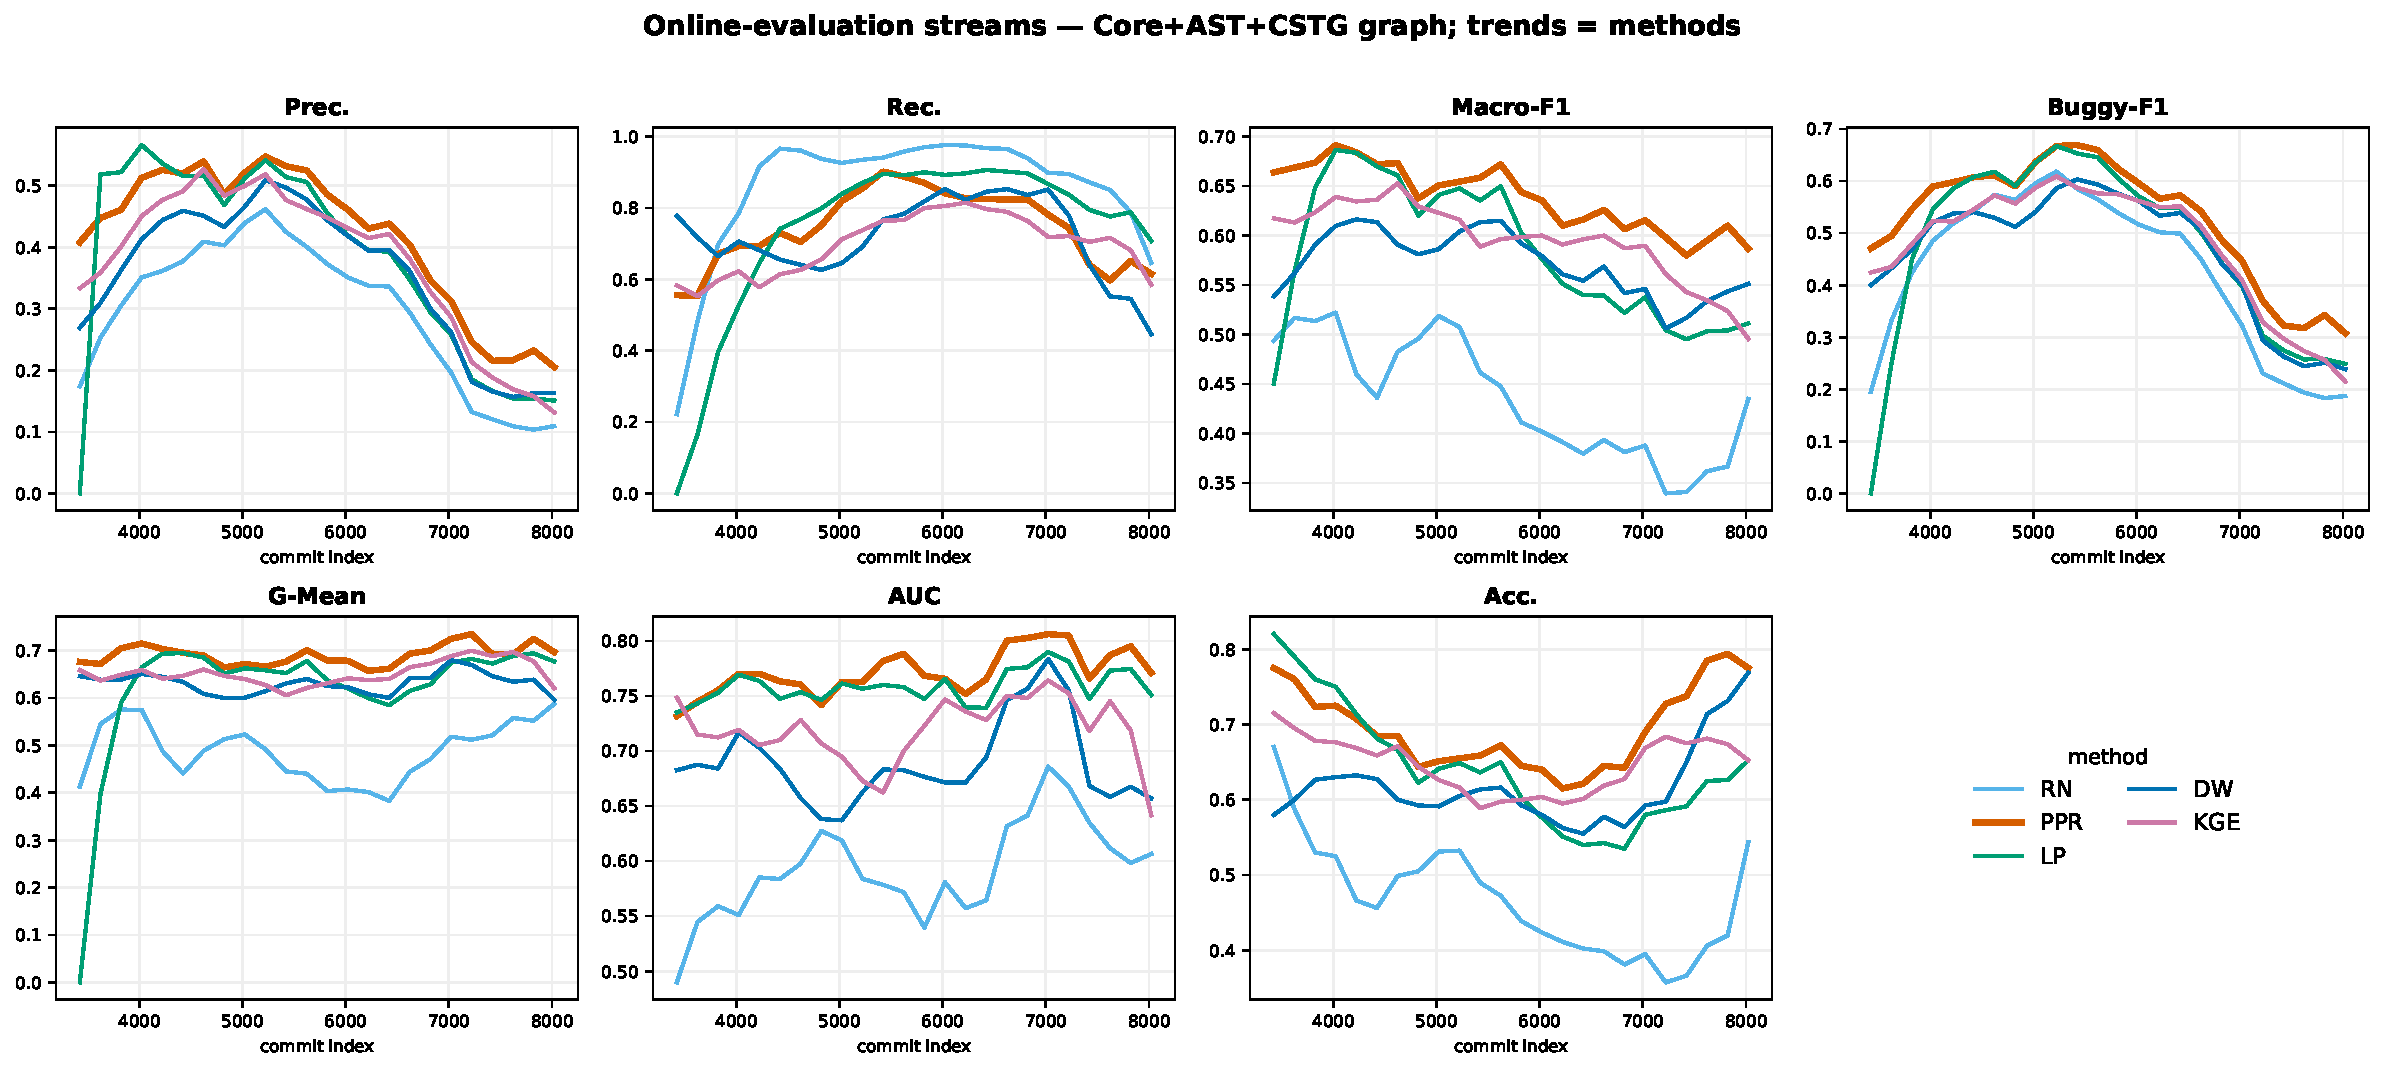
\includegraphics[width=\linewidth]{v4/final/fig_final_bygraph_final}
		\caption{Online-evaluation streams on the final \emph{Core$+$AST$+$CSTG} graph:
		each panel is one of the seven metrics over the commit stream, with the five
		methods as trends (PPR in bold). PPR leads throughout on the balanced metrics.}
		\label{fig:v4-final-streams}
	\end{figure}

	\subsection{Choosing the final fusion of the five methods}\label{sec:v4-finalfusion}
	Having fixed the five methods and the final graph, we choose how to \emph{fuse}
	them (\code{inference/run\_final\_fusion.py}). We stack the five methods'
	probabilities with a prequential logistic regression and evaluate \textbf{all
	$2^5-1=31$ combinations} on the final KG (Table~\ref{tab:v4-final-fusion-ablation}).
	The final fusion is picked to balance \emph{load} (fewer methods, cheaper online)
	against \emph{performance}, prioritising the two class-balanced metrics
	Macro-F1 and G-Mean: we take the smallest combination whose
	$(\text{Macro-F1}+\text{G-Mean})/2$ is within $0.005$ of the best. This selects
	\textbf{$F=$~RN$+$PPR} --- the relational-neighbour and random-walk methods --- with
	Macro-F1~$0.670$ and G-Mean~$0.731$; adding the remaining three methods does not
	improve the balance (the five-method fusion reaches only $0.695$ versus $F$'s
	$0.701$), so two methods suffice.

	\begin{table}[H]
\centering \scriptsize
\caption{All $2^5-1=31$ fusions of the five graph-inference methods on the final Core+AST+CSTG graph (prequential LR stacking), ranked by $(\text{Macro-F1}+\text{G-Mean})/2$. The chosen fusion $F=$\,RN$+$PPR --- the fewest methods within $0.005$ of the best balance --- is highlighted.}
\label{tab:v4-final-fusion-ablation}
\begin{tabular}{rlccrrrrrrr}
\toprule
\# & Fusion & $k$ & bal. & Prec. & Rec. & Macro-F1 & Buggy-F1 & G-Mean & AUC & Acc. \\
\midrule
\textbf{1} & \textbf{RN+PPR} & \textbf{2} & \textbf{0.701} & \textbf{0.443} & \textbf{0.802} & \textbf{0.670} & \textbf{0.571} & \textbf{0.731} & \textbf{0.787} & \textbf{0.701} \\
2 & RN+PPR+LP & 3 & 0.698 & 0.437 & 0.811 & 0.666 & 0.568 & 0.729 & 0.788 & 0.694 \\
3 & RN+PPR+LP+DW+KGE & 5 & 0.695 & 0.442 & 0.767 & 0.668 & 0.561 & 0.723 & 0.787 & 0.702 \\
4 & RN+PPR+LP+KGE & 4 & 0.691 & 0.445 & 0.729 & 0.668 & 0.553 & 0.714 & 0.783 & 0.707 \\
5 & RN+PPR+LP+DW & 4 & 0.690 & 0.436 & 0.765 & 0.663 & 0.556 & 0.718 & 0.788 & 0.696 \\
6 & PPR & 1 & 0.689 & 0.431 & 0.787 & 0.659 & 0.557 & 0.719 & 0.782 & 0.689 \\
7 & RN+LP+DW+KGE & 4 & 0.688 & 0.437 & 0.747 & 0.662 & 0.552 & 0.714 & 0.773 & 0.699 \\
8 & RN+PPR+DW+KGE & 4 & 0.686 & 0.432 & 0.760 & 0.658 & 0.551 & 0.714 & 0.783 & 0.692 \\
9 & PPR+LP+DW+KGE & 4 & 0.685 & 0.436 & 0.732 & 0.661 & 0.547 & 0.710 & 0.782 & 0.699 \\
10 & PPR+LP+DW & 3 & 0.684 & 0.425 & 0.792 & 0.653 & 0.553 & 0.715 & 0.783 & 0.682 \\
11 & PPR+DW+KGE & 3 & 0.683 & 0.430 & 0.753 & 0.656 & 0.547 & 0.710 & 0.774 & 0.691 \\
12 & RN+PPR+KGE & 3 & 0.683 & 0.433 & 0.732 & 0.658 & 0.544 & 0.708 & 0.777 & 0.696 \\
13 & RN+PPR+DW & 3 & 0.683 & 0.428 & 0.756 & 0.655 & 0.547 & 0.710 & 0.780 & 0.689 \\
14 & PPR+LP & 2 & 0.683 & 0.420 & 0.820 & 0.649 & 0.555 & 0.716 & 0.781 & 0.674 \\
15 & PPR+LP+KGE & 3 & 0.680 & 0.428 & 0.737 & 0.654 & 0.542 & 0.706 & 0.775 & 0.691 \\
16 & LP+DW+KGE & 3 & 0.679 & 0.427 & 0.733 & 0.653 & 0.540 & 0.704 & 0.768 & 0.690 \\
17 & RN+LP+KGE & 3 & 0.677 & 0.421 & 0.756 & 0.648 & 0.541 & 0.705 & 0.764 & 0.681 \\
18 & PPR+KGE & 2 & 0.677 & 0.425 & 0.730 & 0.651 & 0.537 & 0.702 & 0.764 & 0.688 \\
19 & LP+DW & 2 & 0.673 & 0.412 & 0.792 & 0.641 & 0.542 & 0.705 & 0.765 & 0.668 \\
20 & RN+LP & 2 & 0.673 & 0.410 & 0.816 & 0.639 & 0.546 & 0.707 & 0.765 & 0.663 \\
21 & RN+LP+DW & 3 & 0.672 & 0.412 & 0.783 & 0.641 & 0.540 & 0.703 & 0.769 & 0.669 \\
22 & PPR+DW & 2 & 0.670 & 0.413 & 0.759 & 0.641 & 0.535 & 0.699 & 0.770 & 0.672 \\
23 & RN+DW+KGE & 3 & 0.669 & 0.411 & 0.769 & 0.639 & 0.535 & 0.699 & 0.760 & 0.669 \\
24 & LP+KGE & 2 & 0.665 & 0.407 & 0.758 & 0.635 & 0.530 & 0.694 & 0.757 & 0.666 \\
25 & DW+KGE & 2 & 0.664 & 0.413 & 0.713 & 0.640 & 0.523 & 0.689 & 0.749 & 0.677 \\
26 & RN+KGE & 2 & 0.660 & 0.404 & 0.741 & 0.632 & 0.523 & 0.688 & 0.741 & 0.664 \\
27 & RN+DW & 2 & 0.652 & 0.395 & 0.745 & 0.623 & 0.516 & 0.681 & 0.737 & 0.653 \\
28 & LP & 1 & 0.633 & 0.374 & 0.774 & 0.600 & 0.505 & 0.666 & 0.736 & 0.623 \\
29 & KGE & 1 & 0.628 & 0.371 & 0.739 & 0.598 & 0.494 & 0.659 & 0.711 & 0.625 \\
30 & DW & 1 & 0.624 & 0.367 & 0.747 & 0.593 & 0.492 & 0.656 & 0.711 & 0.618 \\
31 & RN & 1 & 0.516 & 0.305 & 0.855 & 0.479 & 0.449 & 0.552 & 0.653 & 0.480 \\
\bottomrule
\end{tabular}
\end{table}

	\begin{figure}[H]
		\centering
		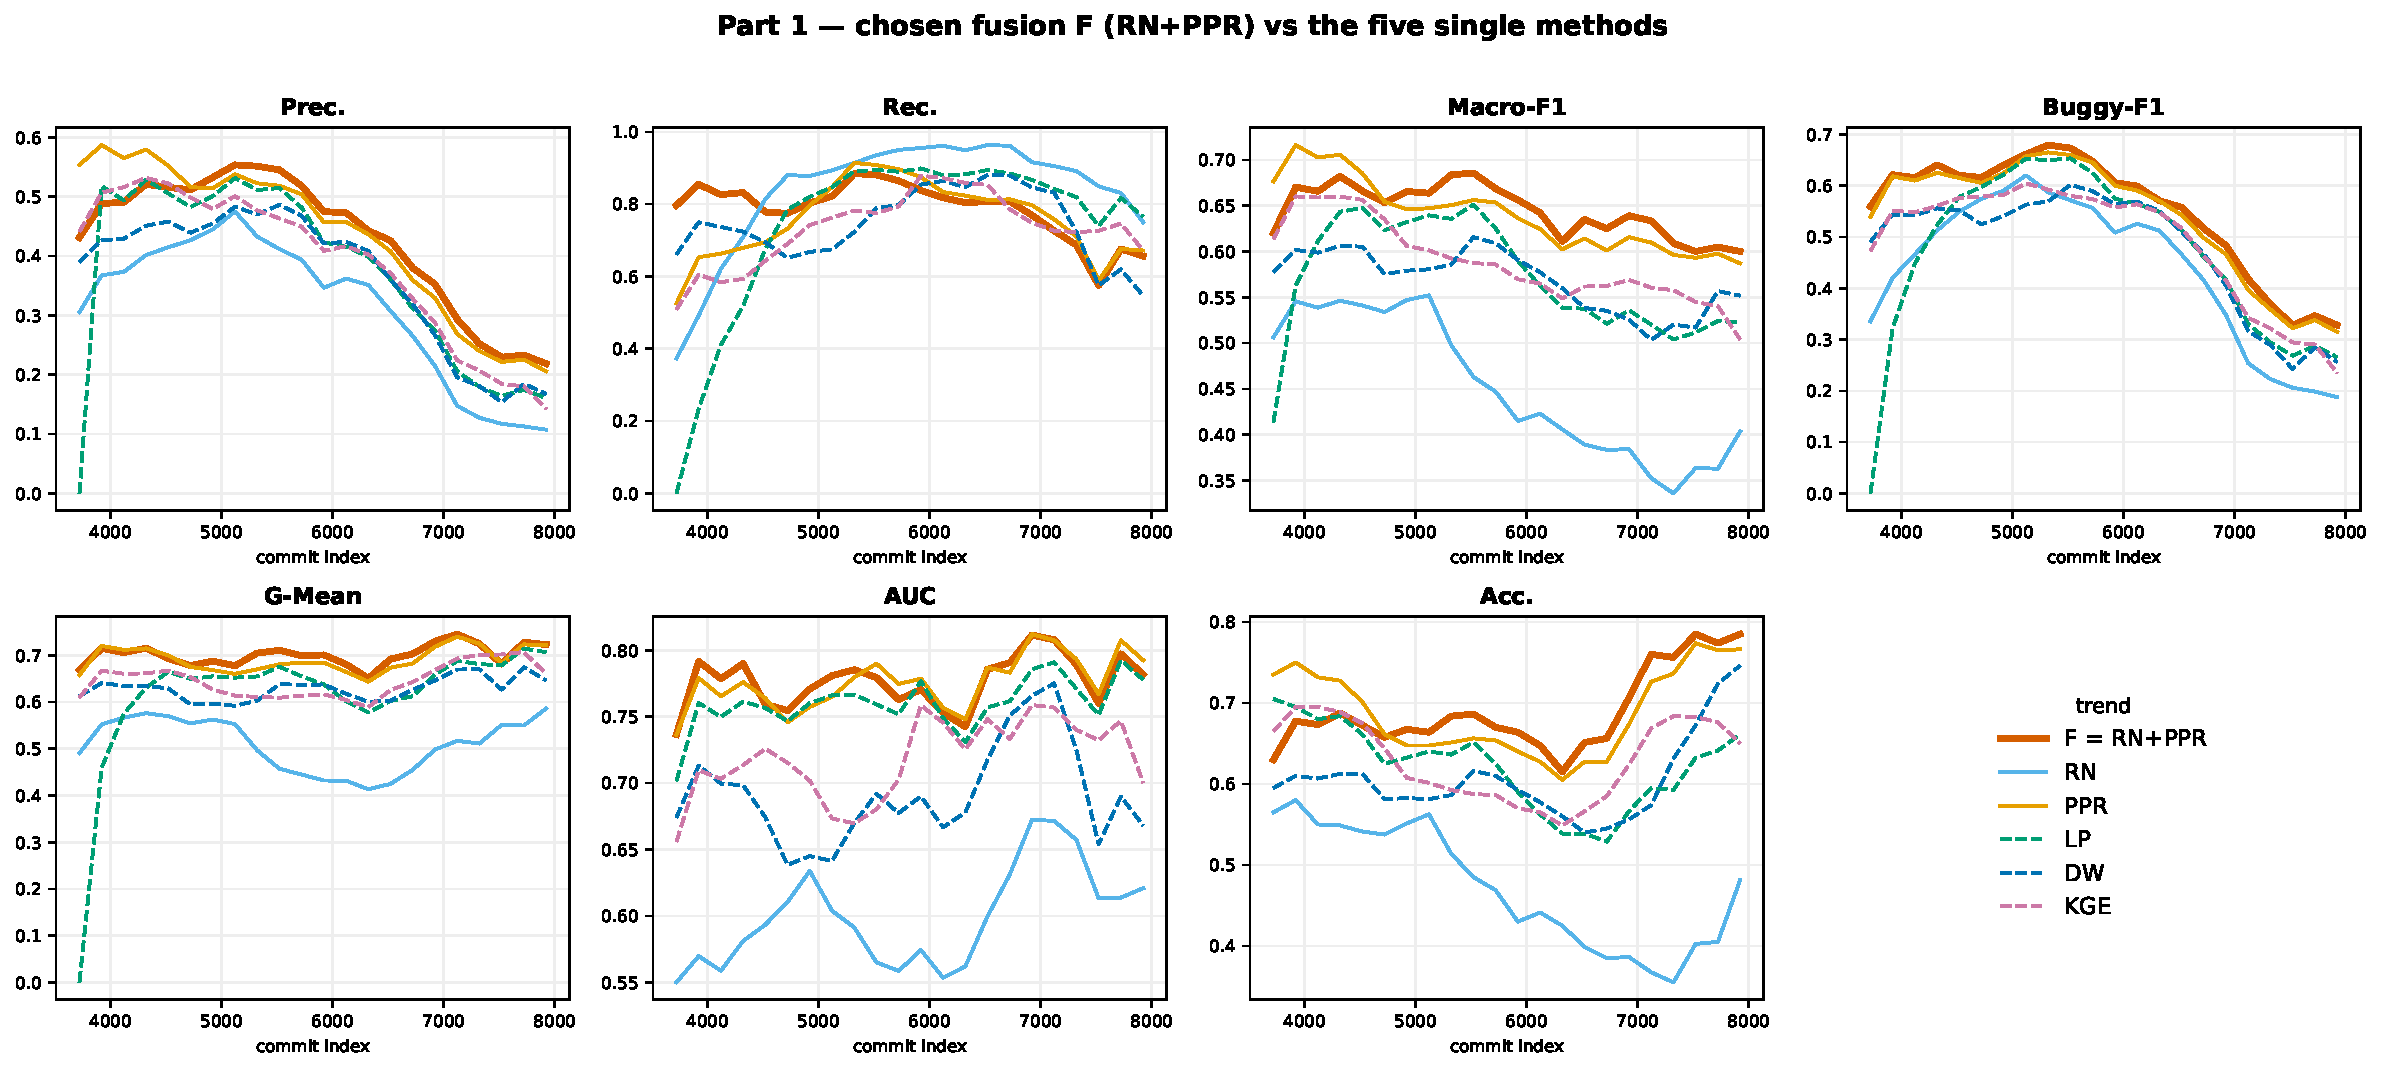
\includegraphics[width=\linewidth]{v4/final/fig_final_fusion_part1}
		\caption{Online-evaluation streams of the chosen fusion $F=$~RN$+$PPR (bold)
		against the five single methods, one panel per metric. $F$ tracks at or above
		the best single method throughout.}
		\label{fig:v4-final-fusion-part1}
	\end{figure}

	\paragraph{What the $G$ channel is.} To avoid confusion, $G$ is \emph{not} a sixth
	graph-walk method: it is a separate \emph{feature-based classifier over the CSTG
	layer}, whose predicted probability is stacked into the fusion by the same
	prequential logistic regression used to combine the five methods
	(\code{inference/run\_final\_fusion.py}, using
	\code{cstg\_online\_features.py}). Per commit, $G$'s feature block concatenates
	(i) a \emph{graph-of-words} text stream --- the commit's message$+$diff terms
	weighted by \emph{TextRank} centrality on its word co-occurrence graph, then hashed;
	(ii) an \emph{NPMI-propagated, past-only term-risk prior} (term bug-risk learned
	from history and diffused over the NPMI term--term graph, refreshed periodically);
	(iii) a $5$-dim \emph{typed-mass} vector over the defect lexicon
	(\{code, bug, action, error, nl\}); and (iv) the message-intent\,/\,code-change
	\emph{consistency} features. This is why $G$ is not admissible as a row of the
	five-method $\times$ six-graph table (\S\ref{sec:v4-select5}): it is defined only on
	the CSTG layer and ignores the commit--hub topology the five methods traverse.
	It therefore enters the methodology only at the fusion stage, on top of $F$.

	\paragraph{Adding the CSTG channel and the JIT metrics.} Finally we ask whether
	the explicit CSTG semantic channel ($G$) or the non-graph JIT metrics ($M$) add
	anything on top of $F$ (Table~\ref{tab:v4-final-fusion-gm},
	Figure~\ref{fig:v4-final-fusion-part2}). \textbf{Adding $G$ helps markedly} ---
	Macro-F1 $0.670\!\to\!0.729$, AUC $0.787\!\to\!0.844$, Buggy-F1 $0.571\!\to\!0.621$
	--- even though the final graph already carries CSTG term-hubs, because the
	explicit semantic-text classifier captures signal the walks do not fully exploit
	through topology alone. \textbf{Adding $M$ alone \emph{hurts}} (Macro-F1 drops to
	$0.648$) and contributes nothing over $G$ ($F{+}G{+}M\approx F{+}G$). The deployed
	model is therefore the purely graph-native \textbf{$F+G=$~RN$+$PPR$+$CSTG}, without
	the non-graph JIT metrics.

	\begin{table}[H]
\centering \small
\caption{Effect of appending the CSTG channel ($G$) and the non-graph JIT metrics ($M$) to the chosen graph-method fusion $F=$\,RN$+$PPR on the final KG. Best per column in \textbf{bold}. Adding $G$ helps markedly; adding $M$ alone hurts and adds nothing over $G$.}
\label{tab:v4-final-fusion-gm}
\begin{tabular}{lrrrrrrr}
\toprule
Fusion & Prec. & Rec. & Macro-F1 & Buggy-F1 & G-Mean & AUC & Acc. \\
\midrule
F & 0.443 & \textbf{0.802} & 0.670 & 0.571 & 0.731 & 0.787 & 0.701 \\
F+G & 0.527 & 0.755 & 0.729 & 0.621 & \textbf{0.766} & 0.844 & 0.771 \\
F+M & 0.419 & 0.798 & 0.648 & 0.549 & 0.712 & 0.787 & 0.675 \\
F+G+M & \textbf{0.548} & 0.722 & \textbf{0.736} & \textbf{0.623} & 0.762 & \textbf{0.844} & \textbf{0.784} \\
\bottomrule
\end{tabular}
\end{table}

	\begin{figure}[H]
		\centering
		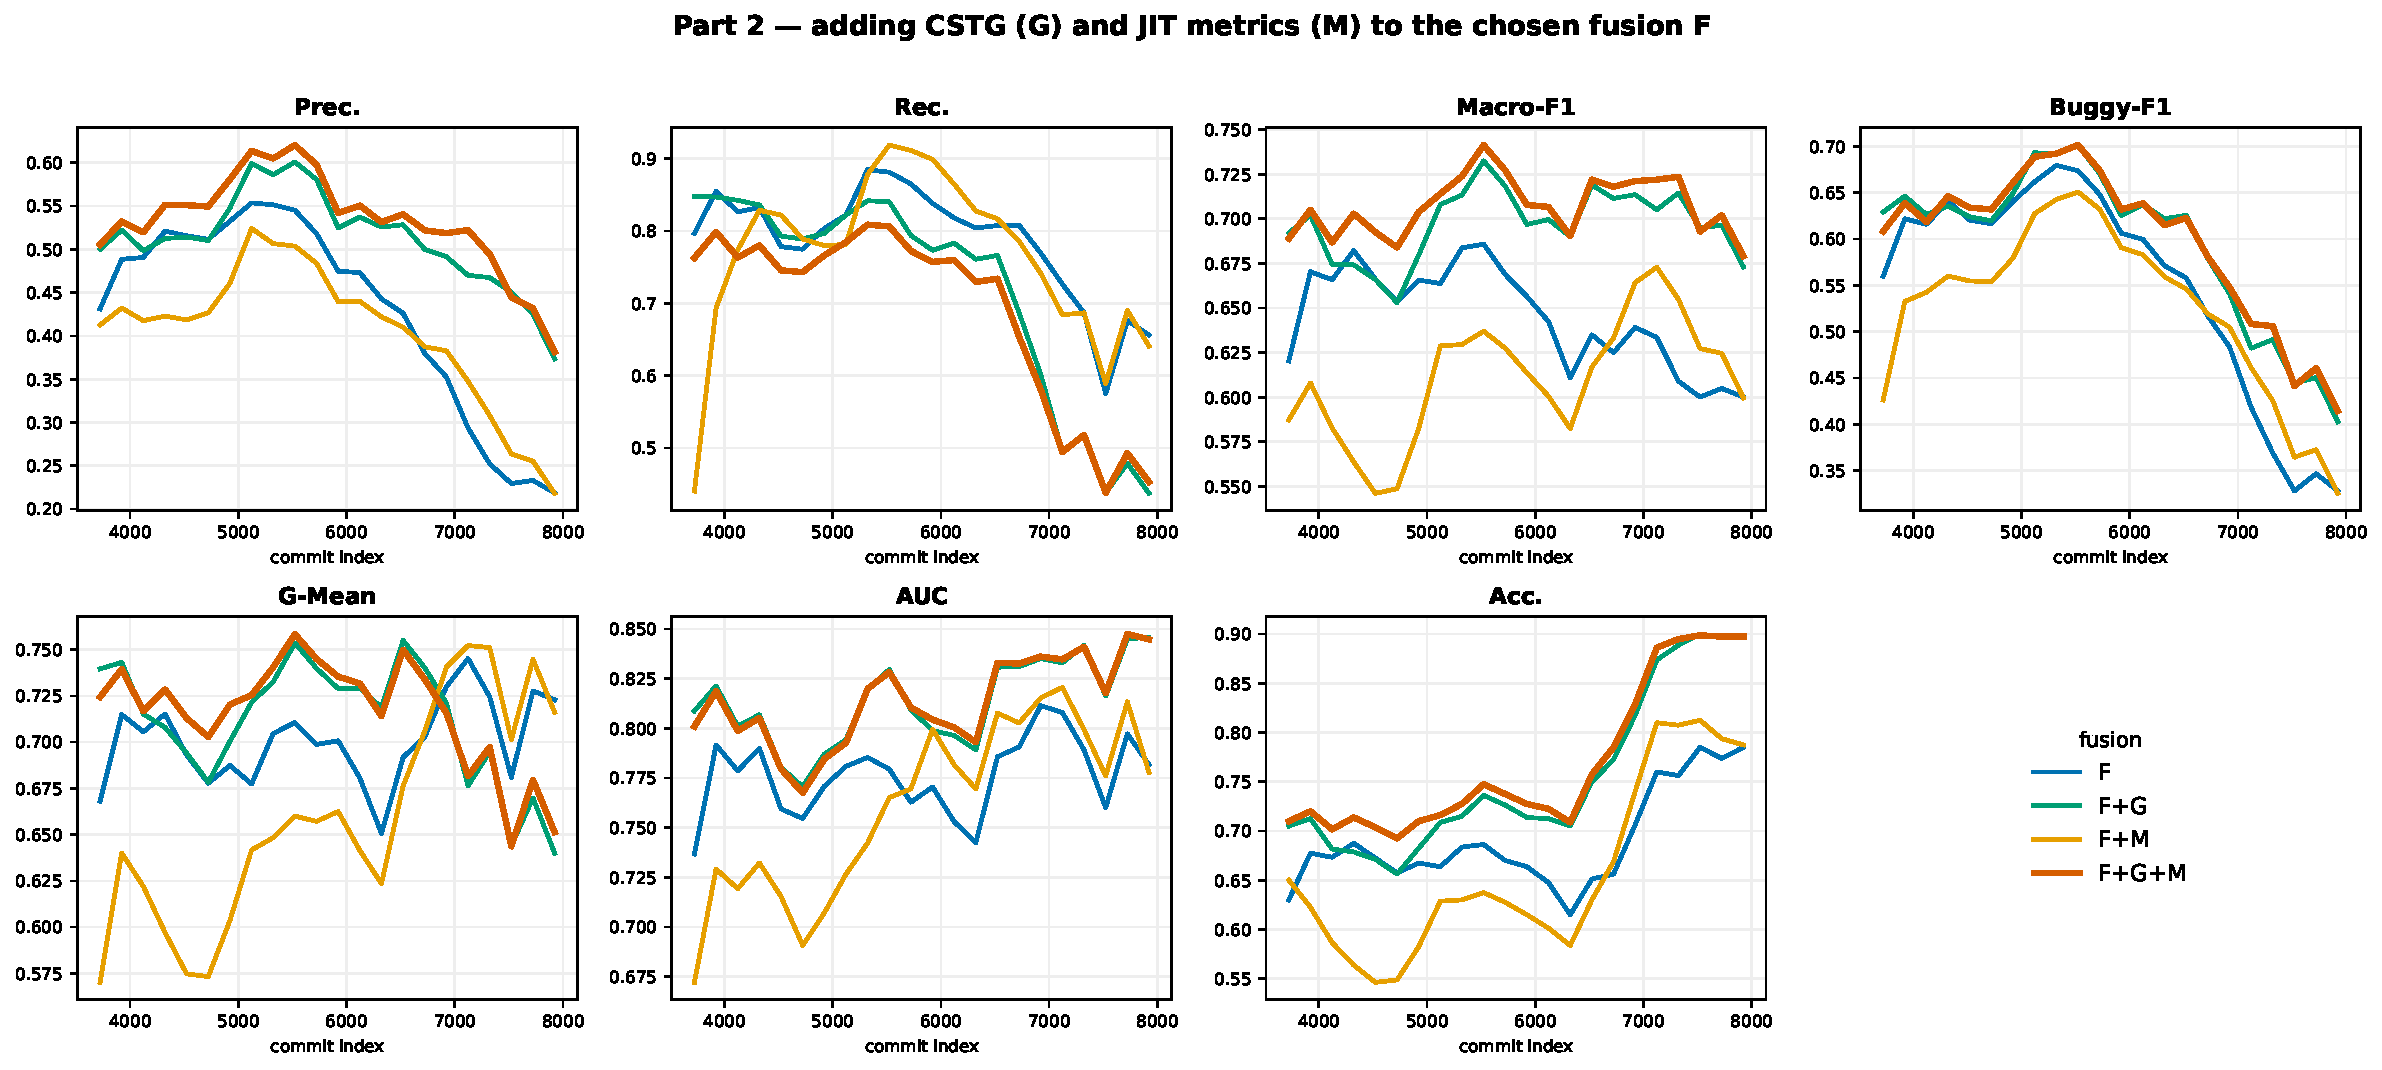
\includegraphics[width=\linewidth]{v4/final/fig_final_fusion_part2}
		\caption{Online-evaluation streams of $F$, $F{+}G$, $F{+}M$ and $F{+}G{+}M$,
		one panel per metric. $F{+}G$ and $F{+}G{+}M$ track together at the top;
		$F{+}M$ is lowest on Macro-F1 and AUC --- the non-graph metrics add noise, not
		signal.}
		\label{fig:v4-final-fusion-part2}
	\end{figure}

	\subsection{Final CSTG questions}\label{sec:v4-cstg-qa}
	Before porting the methodology to other projects, four questions about the
	deployed CSTG channel ($G$) need unambiguous answers --- for our own
	cross-project replication and for a Q1 reviewer auditing the online-JIT claim.
	We answer each directly against the code
	(\code{inference/cstg.py}, \code{cstg\_online\_features.py},
	\code{ingest\_cstg.py}), not from the surrounding prose alone.

	\paragraph{Q1: Is the CSTG's word-graph/statistics update scope the current
	window only, all previous windows, or all data (i.e., is there leakage)?}
	Three distinct mechanisms have three distinct scopes, and only one of them
	looks superficially suspicious:
	\begin{itemize}[nosep,leftmargin=1.4em]
		\item \textbf{Per-commit graph-of-words (TextRank centrality).} Built from
		\emph{that one commit's} tokens only --- no cross-commit state at all.
		\item \textbf{NPMI co-occurrence graph and the propagated term-risk prior.}
		Grown over an \emph{expanding, strictly-past window}: commit $i$ is scored
		using \code{prop} (the last NPMI-propagation refresh, every
		\code{PROP\_REFRESH}$=400$ commits) computed from commits $<i$ only; its own
		tokens are folded into the running counters (\code{tb}, \code{tt}, \code{pair})
		\emph{after} scoring (predict-then-grow, the same protocol as every other
		online signal in the KG). This is never fit on ``all data.''
		\item \textbf{\code{HashingVectorizer} (turns polarity-tagged tokens into
		sparse features).} Applied to the whole document array at once, which can
		look like a full-corpus fit at a glance --- but it is \emph{stateless}: a
		fixed hash function with no learned vocabulary or IDF, so it cannot leak
		information from a later commit into an earlier row. It is included here
		explicitly so the ``applied to all docs'' line in the code is not mistaken
		for a leak on a future audit.
	\end{itemize}
	\textbf{Answer: past-only (expanding window), never all-data.} The controlled-split
	number in Table~\ref{tab:cstg} (\code{cstg.py::CSTG.fit} on a single $70/30$
	\code{train\_idx}) is a separate, explicitly-labelled comparison against the
	published baseline and is \emph{not} the deployed predictor; the deployed
	predictor is the fully prequential path
	(\code{cstg\_online\_features.build\_online\_streams}) reported in
	Table~\ref{tab:cstgonline} and used in $G$ above.

	\paragraph{Q2: How are CSTG nodes/edges constructed, what is the theoretical
	basis, and is it defensible as a completely online, commit-level approach?}
	Terms are tokenised from the commit message and the added/removed diff text
	(camelCase/snake\_case split, stopword and generated-parser-noise removal,
	\code{min\_df}$\ge3$ on past commits only); \edge{MENTIONS} edges connect a commit
	to its top-$20$ terms by \emph{TW-IDF} (TextRank centrality $\times$ IDF, not raw
	frequency); \edge{COOCCURS} edges connect term pairs by \emph{NPMI} over past
	co-occurrence; \edge{GROUNDS\_IN}/\edge{REFERS\_TO} cross-link a code term to the
	\node{ASTNode}/\node{File} it names. Each piece has a standard citation already
	given in \S\ref{sec:cstg}: graph-of-words/TW-IDF (Rousseau \& Vazirgiannis,
	CIKM'13), the NPMI corpus term graph (cf.\ TextGCN, Yao et al., AAAI'19),
	defect-semantic typing, and term-risk propagation (label-propagation /
	spreading-activation). \textbf{This is defensible as a fully online, commit-level
	method} precisely because every statistic used at prediction time is grown
	predict-then-grow from strictly earlier commits and the per-commit graph is
	commit-local (Q1). The one claim we do \emph{not} make is that the
	graph-of-words \emph{centrality math itself} is what wins (Q4) --- the defensible
	claim is that the \emph{structured, typed, code-grounded, online-propagated
	layer} beats the strongest text baseline and adds fusion lift, which is a claim
	about the representation, not about TextRank outperforming term frequency.

	\paragraph{Q3: What are the CSTG node/edge types in detail, and do they make
	sense in a completely online setting?} Node types: \node{Term}
	\{\code{text}, \code{kind}$\in$\{code, bug, action, error, nl\}, \code{risk}\}
	($20{,}377$ in Groovy) and \node{Intent} ($8$, change-intent typing). Edge types:
	\edge{MENTIONS} (Commit$\rightarrow$Term, $188{,}435$), \edge{COOCCURS}
	(Term$\rightarrow$Term, $120{,}340$), \edge{GROUNDS\_IN} (Term$\rightarrow$ASTNode,
	$19{,}315$), \edge{REFERS\_TO} (Term$\rightarrow$File, since deleted as redundant,
	\S\ref{sec:cstgfinal}), and \edge{HAS\_INTENT} (Commit$\rightarrow$Intent,
	$8{,}059$). \edge{MENTIONS}, \edge{HAS\_INTENT} and \edge{GROUNDS\_IN} are all
	written at a commit's arrival from its own text/code, so they are trivially
	online. \edge{COOCCURS} and \node{Term.risk}, however, are corpus-derived and
	evolve over time; \textbf{one distinction is worth stating precisely so it is
	never conflated}: the \emph{Neo4j-ingested} \edge{COOCCURS} graph and
	\code{Term.risk} property (\code{ingest\_cstg.py}) are written \emph{once from
	the final fitted state}, for querying and visualisation
	(Figures~\ref{fig:cstg-cooc}--\ref{fig:cstg-terms}) --- they are a static snapshot,
	not something the online predictor reads. The \emph{deployed feature path}
	(\code{cstg\_online\_features.py}) recomputes its own NPMI graph and propagated
	risk online, from scratch, on past-only counters (Q1). A reviewer inspecting the
	Neo4j schema should not mistake the static visualisation snapshot for the online
	predictor's state.

	\paragraph{Q4: In the CSTG ablation, why does plain TF-IDF outperform the full
	CSTG, and is this a weakness?} It is already reported honestly
	(\S\ref{sec:cstg}, Figure~\ref{fig:cstg-abl}) and is not a weakness once the
	comparison is read at the right granularity, but it is the single most
	reviewer-sensitive result in this layer, so we restate it precisely here and
	close the one gap the original ablation had: a \emph{same-learner},
	matched-vocabulary TF-IDF row (\code{scalability/collect\_cstg\_ablation.py},
	Table~\ref{tab:cstg-ablation}, Figure~\ref{fig:cstg-ablation-internal}).
	\emph{Under a linear learner} (the original component-isolation ablation,
	right panel of Figure~\ref{fig:cstg-ablation-internal}): graph-of-words
	weighting alone (TW-IDF) reaches ROC $0.746$, which does \emph{not} beat plain
	TF-IDF ($0.769$); adding the NPMI-propagated prior recovers only a little
	($0.752$). \emph{Under the matched, non-linear learner} (Random Forest, left
	panel): the gap essentially closes --- plain TF-IDF ($0.818$), TW-IDF
	($0.817$), and the full CSTG ($0.821$) are within noise of one another; only
	\textbf{JIT $+$ full CSTG} ($0.827$) clears the published external baseline
	($0.813$) by a margin worth reporting. \textbf{This changes the precise claim
	we make, and we state it honestly:} the full CSTG representation's advantage
	over a plain bag-of-words baseline, \emph{on this controlled batch split, under
	a matched learner, is small} --- the decisive wins for CSTG are (i)~combining
	with the JIT metrics (which plain TF-IDF was never evaluated with in the
	published baseline) and, far more importantly, (ii)~the true online protocol,
	where CSTG-alone reaches ROC $0.821$ / PR-AUC $0.588$
	(Table~\ref{tab:cstgonline}) because plain TF-IDF has no relational-propagation
	or recency mechanism to draw on across the commit stream --- an advantage a
	single static batch split cannot exercise. \textbf{Two honest consequences we
	act on:} (i)~we never claim ``TextRank-weighting beats term-frequency-weighting
	on this batch split'' --- the matched-learner result shows they are
	statistically indistinguishable here; the defensible claim is that the
	structured, typed, propagated, \emph{online} layer beats a flat bag-of-words
	baseline where it matters, i.e.\ under the deployment protocol; (ii)~the
	original component-isolation ablation mixed a linear learner (for component
	isolation) with a non-linear learner (for the full-representation number),
	which was a fair within-component comparison but not a fair TW-IDF-vs-TF-IDF
	comparison under one learner --- Table~\ref{tab:cstg-ablation} now reports both
	on record so neither the batch-split similarity nor the online-protocol
	advantage can be selectively quoted out of context.

	% Auto-generated -- do not edit by hand.
\begin{table}[t]
\centering
\caption{CSTG internal-layer ablation on the controlled split (train first
$70\%$, test last $15\%$; test bug rate $0.075$).
\textbf{Top block (matched RF learner):} the fair, same-learner comparison this
section's Q4 discussion calls for --- plain TF-IDF vs.\ the graph-of-words (TW-IDF)
representation vs.\ the full CSTG, all under Random Forest. \textbf{Bottom block
(balanced LR):} the original component-isolation ablation, showing each piece's
\emph{marginal} contribution under a linear model. Popt/ACC@20 are effort-aware
metrics (\texttt{effort\_metrics.py}).}
\label{tab:cstg-ablation}
\begin{tabular}{@{}lrrrrr@{}}
\toprule
\textbf{Component} & \textbf{ROC} & \textbf{PR} & \textbf{F1} & \textbf{$P_{\mathrm{opt}}$} & \textbf{ACC@20}\\
\midrule
\multicolumn{6}{@{}l}{\textit{Matched-learner comparison (Random Forest)}}\\
Plain TF-IDF (bag-of-words) [RF] & .818 & .352 & .375 & .821 & .648 \\
TW-IDF (graph-of-words) [RF] & .817 & .296 & .391 & .833 & .648 \\
Full CSTG (+prior+typed) [RF] & .821 & .302 & .402 & .835 & .659 \\
JIT + full CSTG [RF] & .827 & .314 & .390 & .840 & .670 \\
\midrule
\multicolumn{6}{@{}l}{\textit{Component isolation (balanced Logistic Regression)}}\\
(a) Plain TF-IDF (bag-of-words) [LR] & .769 & .268 & .223 & .812 & .615 \\
(b) TW-IDF (graph-of-words) [LR] & .746 & .171 & .216 & .803 & .582 \\
(c) NPMI-propagated prior alone & .723 & .149 & .000 & .785 & .571 \\
(d) TW-IDF + prior [LR] & .752 & .188 & .211 & .805 & .593 \\
(e) Full CSTG (+typed) [LR] & .767 & .176 & .238 & .810 & .604 \\
\midrule
\textit{published diff-text TF-IDF-768D RF (external baseline)} & \textit{0.813} & --- & \textit{0.321} & --- & ---\\
\bottomrule
\end{tabular}
\end{table}


	\begin{figure}[H]\centering
		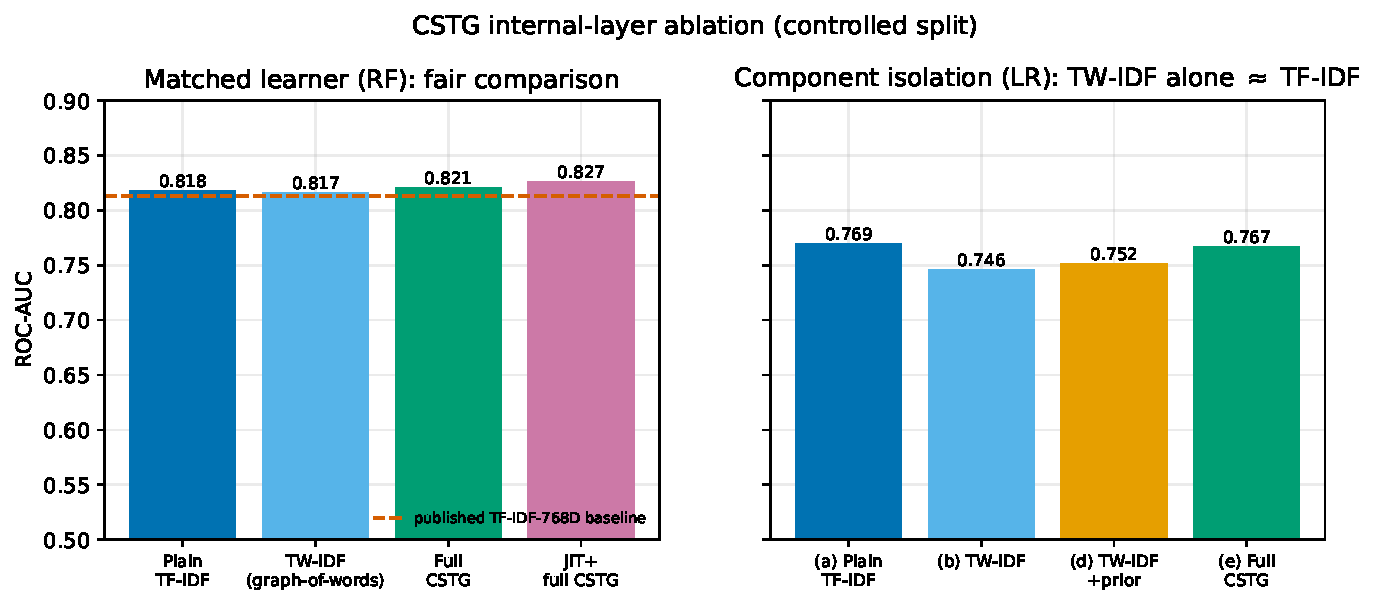
\includegraphics[width=\linewidth]{v4/scalability/fig_cstg_ablation}
		\caption{CSTG internal-layer ablation on the controlled split. \textbf{Left:}
		matched Random-Forest comparison --- plain TF-IDF, TW-IDF and the full CSTG
		are statistically close; only JIT$+$CSTG clears the published baseline
		(dashed). \textbf{Right:} the original balanced-LR component-isolation view,
		where TW-IDF alone $\approx$ TF-IDF. Read together, the two panels show the
		CSTG's batch-split edge is modest and the layer's real advantage is realised
		online (Table~\ref{tab:cstgonline}), not in this static
		comparison.}\label{fig:cstg-ablation-internal}
	\end{figure}

	\paragraph{Q5: How do the five graph-inference methods behave on the CSTG's own
	graph, layer by layer, and how do they compare to the $G$ feature channel?}
	The batch ablation above treats the CSTG as a \emph{feature matrix}. But the
	CSTG is also a \emph{graph} --- \node{Commit}$\rightarrow$\node{Term} mentions,
	\node{Term}$\leftrightarrow$\node{Term} NPMI edges, typed terms --- so we run the
	same five final graph-inference methods (RN, PPR, LP, DW, KGE) over it, fully
	online, exactly as in the V4 subgraph family, to see which \emph{separated CSTG
	layer} carries the signal and how the graph-native methods compare to the
	feature-based $G$ channel (\code{scalability/cstg\_online\_graph\_ablation.py},
	Table~\ref{tab:cstg-graph-ablation}, Figure~\ref{fig:cstg-graph-ablation}). Each
	column adds one CSTG mechanism on top of the Core file/developer graph: unweighted
	term hubs (\edge{MENTIONS}), TW-IDF-weighted term hubs, the \edge{COOCCURS} NPMI
	term--term edges (so the walks diffuse through the semantic graph), and finally
	term-kind typing (the full CSTG). Three findings, all reported honestly:
	\begin{itemize}[nosep,leftmargin=1.4em]
		\item \textbf{PPR is the best graph method, and it is the plain term hubs ---
		not the weighting or the higher-order structure --- that help it.} PPR rises
		from AUC $0.728$ (Core) to its \emph{best} $0.757$ (MCC $0.280\!\to\!0.300$)
		simply by adding \emph{unweighted} \edge{MENTIONS} term hubs. This is
		consistent with PPR being the strongest cell on every graph in the V4 study:
		what the CSTG contributes to the walk is the commit--term connectivity itself.
		\item \textbf{Neither TW-IDF weighting nor the higher-order graph structure
		adds anything for the graph methods --- if anything they slightly hurt.}
		TW-IDF-weighting the term hubs \emph{lowers} PPR to AUC $0.743$, and adding the
		\edge{COOCCURS} NPMI edges and term-kind typing leaves it flat ($0.744$).
		For random-walk and embedding methods the raw term connectivity already
		carries the signal; re-weighting by centrality and diffusing through the
		term--term graph do not add separable information --- an honest null result for
		the higher-order graph mechanisms in this online, prediction-time setting.
		\item \textbf{The $G$ feature classifier beats every graph method on the same
		CSTG signal} (AUC $0.789$ vs.\ PPR's best $0.757$; MCC $0.320$ vs.\ $0.300$).
		This is the decisive result and it \emph{validates the deployed design}: the
		CSTG's semantic evidence is better exploited by an explicit feature classifier
		($G$, fused on top of $F$) than by routing it through graph walks over term
		hubs --- which is exactly why the deployed model is $F{+}G$ with $G$ as a fused
		channel (\S\ref{sec:v4-finalfusion}), rather than folding CSTG hubs into the
		five methods and stopping there.
	\end{itemize}

	% Auto-generated -- do not edit by hand.
\begin{table}[t]
\centering
\caption{CSTG \emph{online graph} ablation: the five final graph-inference methods
(RN, PPR, LP, DW, KGE) run fully online (prequential) over the CSTG's own graph
structure, one column per \emph{separated} CSTG hub-graph layer and one for the
full CSTG --- Core (file/dev hubs only), $+$MENTIONS (unweighted term hubs),
$+$TW-IDF (TextRank-weighted term hubs), $+$COOCCURS (adds the NPMI term--term
graph so walks diffuse through it), and Full CSTG (adds term-kind-typed edges).
The \emph{G (feature clf.)} row is the graph-independent CSTG feature classifier
under the same online protocol, for reference. All seven metrics are computed by
\texttt{online\_jit.final\_metrics}; five are shown here
(\texttt{scalability/cstg\_online\_graph\_ablation.py}).}
\label{tab:cstg-graph-ablation}
\begin{tabular}{@{}lrrrrr@{}}
\toprule
Method & Core & +MENT. & +TW-IDF & +COOCC. & Full \\
\midrule
\multicolumn{6}{@{}l}{\textit{Buggy-F1}}\\
RN & .493 & .470 & .455 & .455 & .455 \\
PPR & .499 & .526 & .516 & .514 & .514 \\
LP & .459 & .453 & .475 & .475 & .475 \\
DW & .396 & .449 & .445 & .445 & .445 \\
KGE & .439 & .453 & .453 & .453 & .453 \\
\;\;G (feature clf.) & \multicolumn{5}{c}{.550} \\
\midrule
\multicolumn{6}{@{}l}{\textit{Macro-F1}}\\
RN & .603 & .519 & .510 & .510 & .510 \\
PPR & .600 & .636 & .615 & .617 & .617 \\
LP & .518 & .487 & .524 & .524 & .524 \\
DW & .407 & .550 & .533 & .533 & .533 \\
KGE & .479 & .487 & .487 & .487 & .484 \\
\;\;G (feature clf.) & \multicolumn{5}{c}{.659} \\
\midrule
\multicolumn{6}{@{}l}{\textit{G-Mean}}\\
RN & .662 & .597 & .586 & .586 & .586 \\
PPR & .665 & .694 & .682 & .681 & .681 \\
LP & .594 & .564 & .604 & .604 & .604 \\
DW & .473 & .612 & .600 & .600 & .600 \\
KGE & .553 & .563 & .563 & .563 & .560 \\
\;\;G (feature clf.) & \multicolumn{5}{c}{.716} \\
\midrule
\multicolumn{6}{@{}l}{\textit{AUC}}\\
RN & .696 & .683 & .674 & .674 & .674 \\
PPR & .728 & .757 & .743 & .744 & .744 \\
LP & .687 & .674 & .679 & .679 & .679 \\
DW & .576 & .657 & .642 & .642 & .642 \\
KGE & .629 & .655 & .655 & .655 & .660 \\
\;\;G (feature clf.) & \multicolumn{5}{c}{.789} \\
\midrule
\multicolumn{6}{@{}l}{\textit{MCC}}\\
RN & .131 & .000 & .017 & .017 & .017 \\
PPR & .280 & .300 & .291 & .290 & .290 \\
LP & .144 & .025 & .041 & .041 & .041 \\
DW & .098 & .209 & .187 & .187 & .187 \\
KGE & .170 & .199 & .199 & .199 & .199 \\
\;\;G (feature clf.) & \multicolumn{5}{c}{.320} \\
\bottomrule
\end{tabular}
\end{table}


	\begin{figure}[H]\centering
		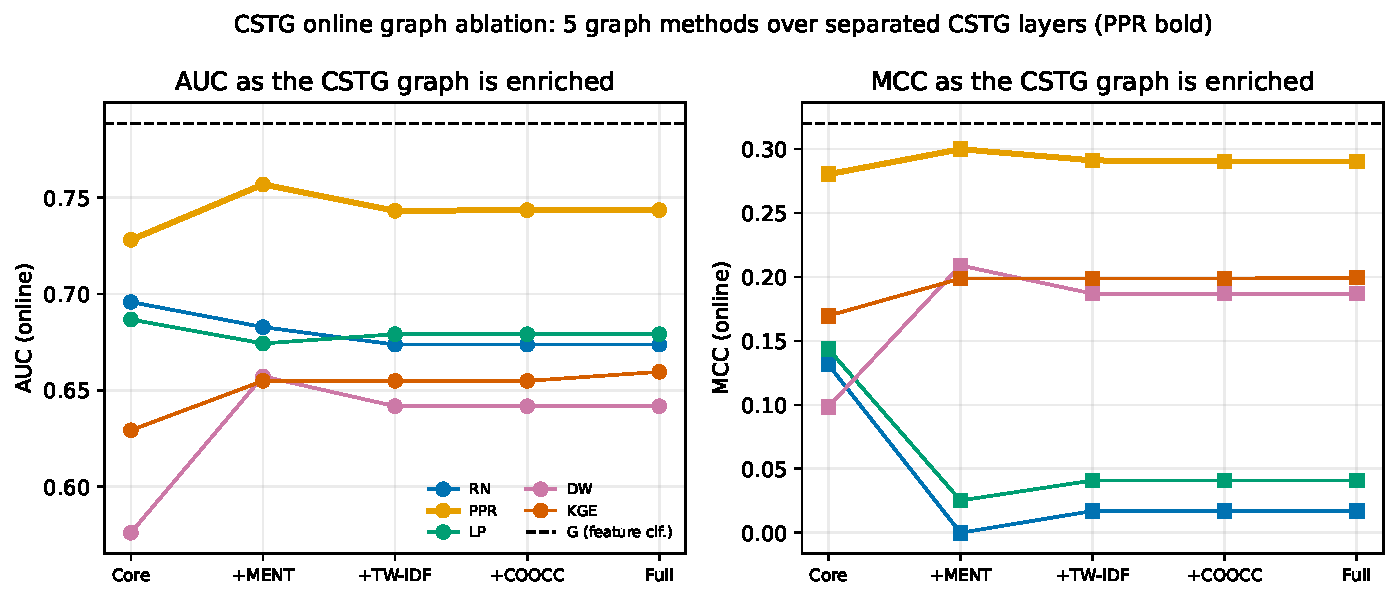
\includegraphics[width=\linewidth]{v4/scalability/fig_cstg_graph_ablation}
		\caption{CSTG online graph ablation. Each panel tracks a metric as the CSTG
		graph is enriched Core\,$\rightarrow$\,$+$MENTIONS\,$\rightarrow$\,$+$TW-IDF\,
		$\rightarrow$\,$+$COOCCURS\,$\rightarrow$\,Full, for the five graph methods
		(PPR bold); the dashed line is the graph-independent $G$ feature classifier.
		Plain (unweighted) term hubs give PPR its best result; TW-IDF weighting and
		the higher-order graph structure do not help the graph methods; and $G$ sits
		above every graph method --- the reason the deployed model fuses $G$
		explicitly rather than relying on CSTG hubs alone.}\label{fig:cstg-graph-ablation}
	\end{figure}

	% =======================================================================
	\section{Scalability, Complexity and Statistical Analysis}\label{sec:scal}
	% =======================================================================
	The V4 study establishes \emph{which} representation and methods are best; this
	section establishes that the resulting system is \emph{scalable, cheap to run,
	and statistically sound}. We analyse all four phases --- the Core graph, the
	structural-subgraph family, the CSTG layer, and the five graph-inference methods
	with their deployed fusion --- along four axes: a statistical profile of the final
	graph, per-commit growth, build/predict complexity, and significance testing of
	the headline comparisons. Every number here is obtained \textbf{without rebuilding
	the knowledge graph}: final sizes and growth come from read-only snapshots of the
	assembled database, prediction latency from replaying the cached graph family
	in-memory, and build cost from a sampled replay of the real parse-and-diff work.
	The analysis code is in \code{scalability/} and the companion notebook is
	\code{experiments/notebooks/scalability\_v4.ipynb}.

	\paragraph{Reproducibility on new projects.} The per-commit build wall-clock was
	not persisted for the Groovy build (only deltas are stored). Both online engines
	therefore now accept an opt-in \code{--timing-log} flag that appends one row per
	commit (file actions, delta counts, wall-ms) at build time; it is off by default,
	so the Groovy database is untouched, and on for any \emph{new} project it captures
	the full per-commit timing natively.

	\subsection{Statistical profile of the final graph}\label{sec:scal-profile}
	Table~\ref{tab:scal-profile} profiles every materialised layer. Beyond the raw
	scale (recovered exactly: AST $3{,}699{,}439$ nodes, matching
	Table~\ref{tab:v4-layers}), two distributional facts matter. First, per-file sizes
	are highly skewed (Gini $\approx0.6$--$0.7$): a few large files dominate each
	layer, as expected of real software. Second, the per-commit change size is
	\textbf{heavy-tailed} on every layer, with a maximum-likelihood power-law exponent
	$\alpha\in[2.0,2.3]$ --- the regime ($2<\alpha<3$) in which the mean is finite but
	the variance is not, i.e.\ most commits are tiny and a few are enormous
	(Figure~\ref{fig:scal-degree}). This is precisely the distribution a delta-based
	store is designed for: storage follows the (small, typical) change, not a
	worst-case snapshot. The CSTG layer adds a compact, bounded semantic increment
	($20{,}377$ \node{Term} nodes; ${\approx}20$ \edge{MENTIONS} per commit).

	% Auto-generated by scalability/make_scalability_tables.py -- do not edit by hand.
\begin{table}[t]
\centering
\caption{Statistical profile of each materialised layer of the final knowledge
graph (Groovy, $8{,}059$ commits). \emph{Med.\ nodes/file} and \emph{Gini} describe
the per-file size distribution; $\alpha$ is the MLE power-law exponent of the
per-commit change-token degree (heavy-tailed for $2<\alpha<3$). The CSTG row counts
its \node{Term} nodes and its semantic edges (\edge{MENTIONS}$+$\edge{COOCCURS}$+$\edge{GROUNDS\_IN}).}
\label{tab:scal-profile}
\begin{tabular}{lrrrrrrr}
\toprule
Layer & Nodes & Delta-edges & Node & Token & Med.\ nodes & Gini & $\alpha$ \\
      &       &             & types & types & /file       &      &          \\
\midrule
AST & 3{,}699{,}439 & 3{,}614{,}922 & 136 & 314 & 286 & .78 & 2.05 \\
CFG & 372{,}488 & 408{,}301 & 18 & 53 & 43 & .73 & 2.15 \\
DFG & 469{,}662 & 648{,}553 & 7 & 27 & 34 & .81 & 2.27 \\
PDG & 372{,}488 & 411{,}869 & 18 & 63 & 43 & .73 & 2.17 \\
Token-seq & 257{,}708 & 293{,}287 & 16 & 47 & 25 & .76 & 2.10 \\
\midrule
CSTG & 20{,}377 & 328{,}090 & 5 & -- & -- & -- & -- \\
\bottomrule
\end{tabular}
\end{table}


	\begin{figure}[H]\centering
		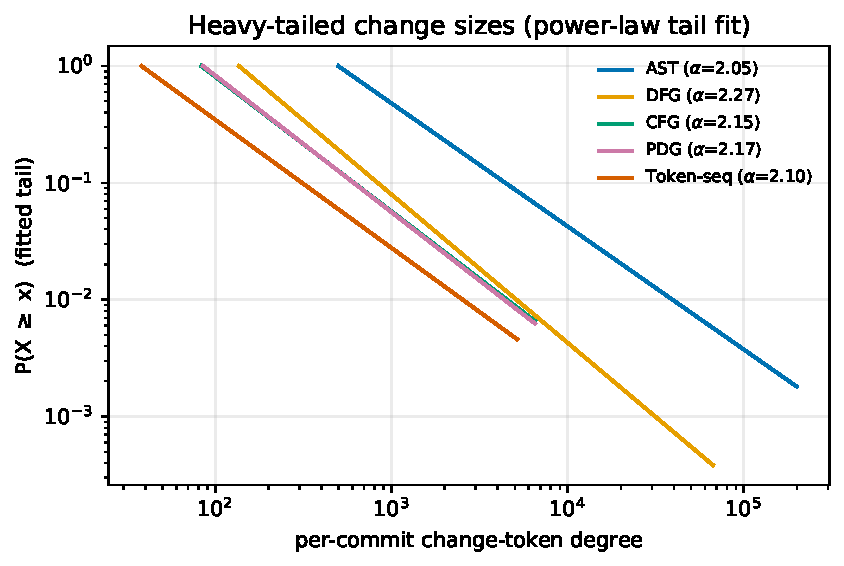
\includegraphics[width=.72\linewidth]{v4/scalability/fig_degree_loglog}
		\caption{Fitted power-law tail of the per-commit change-token degree for each
		layer ($\alpha\in[2.0,2.3]$): change sizes are heavy-tailed everywhere, so
		delta storage cost is dominated by a small number of large commits.}
		\label{fig:scal-degree}
	\end{figure}

	\subsection{Per-commit growth and modification}\label{sec:scal-growth}
	Because commits are ingested in \code{author\_ts} order and only deltas are stored,
	the graph grows with the \emph{amount of change}, not with history length.
	Table~\ref{tab:scal-growth} reports, per layer, the total delta volume, the churn
	ratio (\edge{REMOVES}/\edge{ADDS} $\approx0.4$--$0.5$: the tree mostly grows, with
	substantial but minority deletion), and the buggy-vs-benign change-size gap.
	\textbf{Buggy commits make significantly larger structural changes} on every layer:
	the mean per-commit delta ratio is $2.0$--$2.8\times$ (bootstrap $95\%$ CI excludes
	$1$ throughout) and a one-sided Mann--Whitney test rejects equality with
	$p\ll10^{-90}$ (for AST, $p\approx7\times10^{-133}$). This size separation ---
	visible in Figure~\ref{fig:scal-growth} together with the pronounced yearly bug-rate
	drift --- is the structural basis of the graph's predictive value.

	\begin{table}[t]
	\centering
	\caption{Per-commit growth and modification statistics recovered from the online
		delta stream. \emph{Churn} is \edge{REMOVES}/\edge{ADDS}; buggy/benign columns are
		mean per-commit delta-edges; the ratio carries a bootstrap $95\%$ CI and a
		Mann--Whitney $U$ $p$-value for the (buggy $>$ benign) size separation.}
	\label{tab:scal-growth}
	\begin{tabular}{lrrrrrl}
		\toprule
		Layer & Total & Churn & Med.\ & Buggy & Benign & Ratio [CI] \quad ($p$) \\
		& delta & & /commit & mean & mean & \\
		\midrule
		AST & 3{,}614{,}922 & .44 & 84 & 909 & 366 & 2.48 [1.82,3.48] $<$1e-99 \\
		CFG & 408{,}301 & .51 & 18 & 108 & 53 & 2.03 [1.71,2.41] 3e-91 \\
		DFG & 648{,}553 & .38 & 31 & 208 & 75 & 2.78 [1.88,4.34] $<$1e-99 \\
		PDG & 411{,}869 & .51 & 18 & 109 & 53 & 2.07 [1.74,2.46] 1e-97 \\
		SEQ & 293{,}287 & .53 & 14 & 80 & 39 & 2.05 [1.72,2.43] $<$1e-99 \\
		\bottomrule
	\end{tabular}
\end{table}

	\begin{figure}[H]\centering
		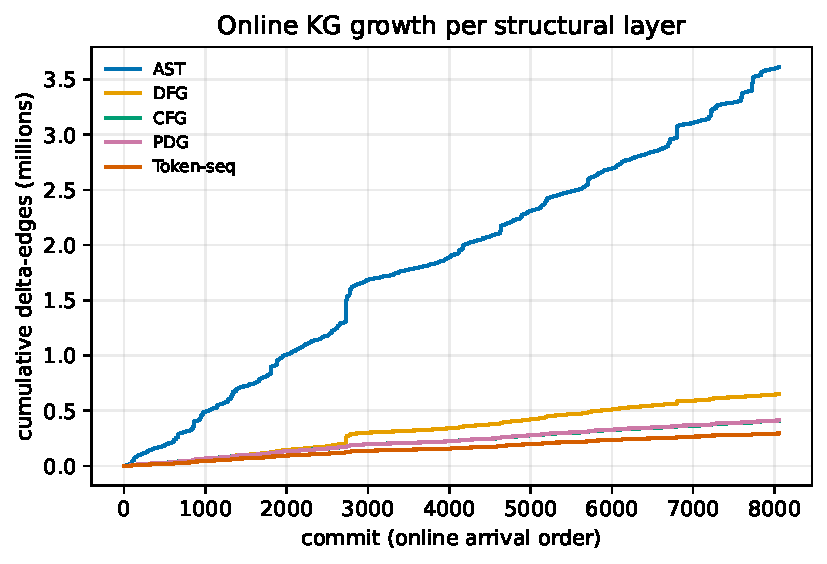
\includegraphics[width=.48\linewidth]{v4/scalability/fig_growth_cumulative}\hfill
		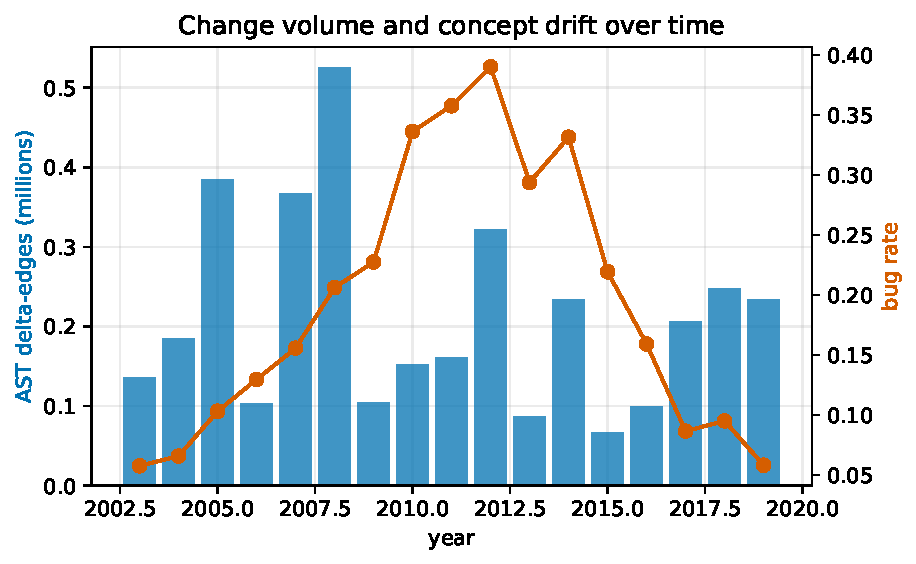
\includegraphics[width=.48\linewidth]{v4/scalability/fig_growth_year}
		\caption{Left: cumulative delta-edges per layer over the commit stream ---
		smooth, near-linear online growth. Right: AST change volume and the yearly bug
		rate, showing the concept drift that motivates the time-aware protocol.}
		\label{fig:scal-growth}
	\end{figure}

	\subsection{Time and space complexity}\label{sec:scal-complexity}
	\paragraph{Build / modify.} Per-commit work is the parse of the changed file(s)
	plus a tree/graph diff against the stored state; space is $O(\text{alive nodes} +
	\text{retained history})$, with per-commit growth $O(\text{change})$ and no
	full-snapshot-per-commit cost. Table~\ref{tab:scal-build} quantifies the CPU
	parse-and-diff cost from a sampled replay of real modified-file pairs (Neo4j write
	I/O excluded --- it is dominated by the schema-index cost documented in
	\S\ref{sec:v4-engine}). The time-vs-file-size fit is near-perfect
	($R^2\approx0.99$), confirming the cost is linear in the amount of code processed;
	AST is ${\approx}20\times$ costlier per file than the coarse layers
	($402$ vs.\ $17$--$25$\,ms), exactly its ${\approx}10\times$ node-granularity plus
	tree-diff overhead (Figure~\ref{fig:scal-cost}, left).

	\paragraph{Prediction.} At deployment the model scores each arriving commit from
	strictly-past state. Table~\ref{tab:scal-latency} gives the median per-commit
	latency of all five methods across the graph family: it grows with graph density
	(e.g.\ PPR $0.035\to0.208$\,ms from Core to the final graph) yet the deployed
	graph-native fusion $F=$~RN$+$PPR stays \textbf{sub-millisecond per commit}
	(${\approx}3{,}200$ commits/s) even on the richest graph. The embedding methods
	(DW, KGE) have negligible per-commit \emph{scoring} cost --- their cost is a bursty
	per-block refit, amortised in Figure~\ref{fig:scal-cost} (right). The whole
	pipeline is comfortably real-time and GPU-free.

	% Auto-generated -- do not edit by hand.
\begin{table}[t]
\centering
\caption{Build/modify cost from a sampled replay of the real parse+diff work
(CPU only; Neo4j write I/O excluded). The high $R^2$ of the time-vs-change-size fit
confirms per-commit work is \emph{linear in the size of the change} (\,$O(\text{change})$\,),
independent of history length. The last column extrapolates the median per-file cost
to the full stream.}
\label{tab:scal-build}
\begin{tabular}{lrrrrr}
\toprule
Layer & \#samp. & Med.\ ms & $R^2$ (nodes) & $R^2$ (delta) & Est.\ total (min) \\
\midrule
AST & 120 & 401.8 & .98 & .11 & 50.4 \\
CFG & 120 & 18.4 & .99 & .06 & 1.9 \\
DFG & 120 & 21.6 & .99 & .12 & 2.2 \\
PDG & 120 & 24.7 & .99 & .06 & 2.6 \\
SEQ & 120 & 17.2 & .98 & .08 & 1.7 \\
\bottomrule
\end{tabular}
\end{table}

	% Auto-generated -- do not edit by hand.
\begin{table}[t]
\centering
\caption{Prediction latency (median ms per commit) of the five final graph-inference
methods across the graph family, at deployment (steady per-commit scoring from
strictly-past state; embedding refit cost is amortised separately). The deployed
graph-native fusion $F=$~RN$+$PPR runs at sub-millisecond per commit even on the
richest final graph.}
\label{tab:scal-latency}
\begin{tabular}{lrrrrrr}
\toprule
Method & Core & +AST & +CFG & +DFG & +PDG & +AST+CSTG \\
\midrule
RN & .006 & .077 & .048 & .043 & .051 & .103 \\
PPR & .035 & .101 & .061 & .056 & .063 & .208 \\
LP & .005 & .020 & .008 & .008 & .008 & .038 \\
DW & .001 & .001 & .001 & .001 & .001 & .001 \\
KGE & .000 & .000 & .000 & .000 & .000 & .000 \\
\midrule
\textbf{$F$=RN+PPR} & .041 & .178 & .109 & .099 & .114 & .311 \\
\bottomrule
\end{tabular}
\end{table}


	\begin{figure}[H]\centering
		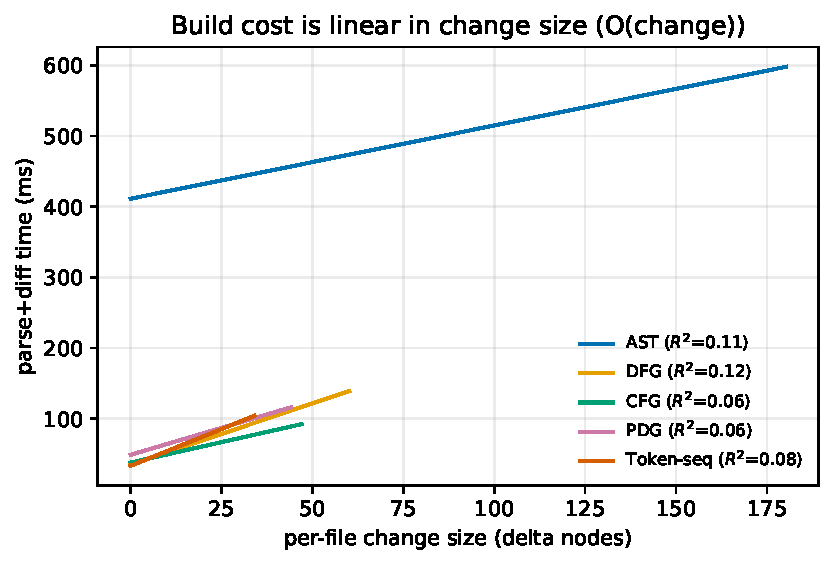
\includegraphics[width=.48\linewidth]{v4/scalability/fig_build_cost}\hfill
		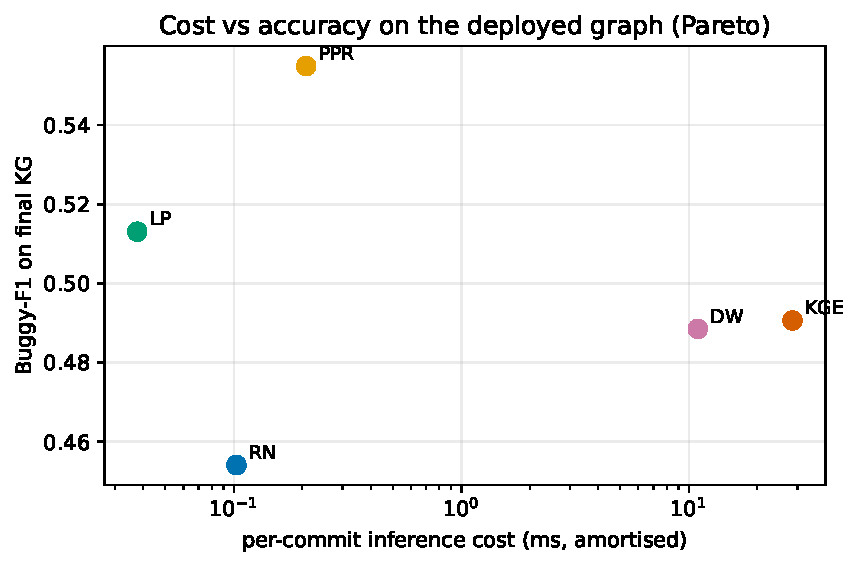
\includegraphics[width=.48\linewidth]{v4/scalability/fig_pareto_cost_accuracy}
		\caption{Left: parse+diff time is linear in change size per layer
		($O(\text{change})$). Right: cost--accuracy Pareto front on the deployed graph
		--- PPR (and the $F=$~RN$+$PPR fusion it anchors) is Pareto-optimal, dominating
		the far costlier embeddings.}
		\label{fig:scal-cost}
	\end{figure}

	\subsection{Statistical significance of the headline comparisons}\label{sec:scal-sig}
	Finally we attach significance to the V4 claims using paired per-commit
	out-of-sample scores, replayed from the cached graph family, with DeLong's test for
	ROC-AUC (Holm-corrected within each family) and a bootstrap for the interval
	estimates (Table~\ref{tab:scal-sig}). Three results hold. \textbf{(i) Graph richness
	helps} the informative methods significantly: PPR, LP and the embeddings all improve
	from Core to the final graph ($\Delta$AUC up to $+0.134$ for DeepWalk,
	$p\approx6\times10^{-34}$), while the one-hop relational neighbour is diluted by the
	extra hubs --- exactly the pattern of \S\ref{sec:v4-finalexp}. \textbf{(ii) PPR is
	significantly the best} method on the final graph (every pairwise
	$\Delta$AUC$>0$, Holm $p\le10^{-16}$). \textbf{(iii) The semantic channel is real}:
	the deployed $F{+}G$ significantly improves every headline metric over $F$
	(ROC $0.787\to0.844$, PR-AUC $0.501\to0.637$, Macro-F1 $0.670\to0.729$). The
	headline accuracy gaps are therefore not noise.

	% Auto-generated -- do not edit by hand.
\begin{table}[t]
\centering
\caption{Statistical significance of the headline V4 comparisons. Rows in the
first two blocks use paired per-commit out-of-sample scores: $\Delta$AUC is the
ROC-AUC difference and $p$ is DeLong's paired test, Holm-corrected within each
block. The last block reports the deployed semantic-channel effect (F$+$G vs.\ F)
as the change in each headline metric from the final fusion run
(\code{run\_final\_fusion.py}).}
\label{tab:scal-sig}
\begin{tabular}{lrl}
\toprule
Comparison & $\Delta$ & $p$ (Holm) / value \\
\midrule
\multicolumn{3}{@{}l}{\textit{Graph richness helps (final graph vs.\ Core), $\Delta$AUC}}\\
RN: final $>$ Core & -0.049 & 9e-6 \\
PPR: final $>$ Core & .051 & 3e-8 \\
LP: final $>$ Core & .048 & 1e-6 \\
DW: final $>$ Core & .134 & 6e-34 \\
KGE: final $>$ Core & .084 & 1e-12 \\
\midrule
\multicolumn{3}{@{}l}{\textit{Best method on the final graph, $\Delta$AUC}}\\
PPR $>$ RN & .133 & 2e-36 \\
PPR $>$ LP & .044 & 2e-18 \\
PPR $>$ DW & .070 & 3e-16 \\
PPR $>$ KGE & .067 & 1e-21 \\
\midrule
\multicolumn{3}{@{}l}{\textit{Deployed semantic channel F$+$G vs.\ F}}\\
F+G $>$ F (ROC-AUC) & .057 & .787$\to$.844 \\
F+G $>$ F (PR-AUC) & .136 & .501$\to$.637 \\
F+G $>$ F (Macro-F1) & .058 & .670$\to$.729 \\
F+G $>$ F (G-Mean) & .034 & .731$\to$.766 \\
\bottomrule
\end{tabular}
\end{table}


	% =======================================================================
	\section{Reproducibility Package and Cross-Project Pipeline}\label{sec:repro}
	% =======================================================================
	The final methodology is packaged as a standalone, publishable code artifact
	(\code{kgcommit\_repro/}) that reconstructs \emph{everything} in this paper ---
	from reading a cloned repository and the ApacheJIT labels, through building the
	full knowledge graph in Neo4j, to running every experiment and rendering every
	table, figure, and notebook --- for \emph{any} Apache project, \textbf{one
	project at a time}. The package deliberately contains \emph{only} the final (V4)
	methodology; the superseded V1--V3 experimentation, legacy builders, and one-off
	audits that appear earlier in this document are excluded. This section documents
	what the package contains, how to run the full pipeline on a new project, where
	each input is read from, and the operational facts a reader must know.

	\subsection{What the package contains}\label{sec:repro-contents}
	The artifact mirrors the three stages of the methodology --- \emph{build},
	\emph{inference}, \emph{analysis} --- as three script folders, plus a
	single-source-of-truth configuration, four thin orchestration drivers, and two
	setup helpers. Every script reads its project-specific values (repository path,
	base commit, label/diff CSVs, output namespace, Neo4j credentials) from one
	module, \code{config/project\_config.py}, which resolves them from a per-project
	registry (\code{config/projects.yaml}) keyed by the \code{KGC\_PROJECT}
	environment variable. Nothing is hard-coded to a single project.

	\paragraph{Build (\code{build/}) --- the ten ordered steps that grow the graph.}
	\begin{description}[nosep,leftmargin=1.2em]
		\item[\code{build\_file\_ast\_graphs.py}] parses every \code{.java} file at the
		base commit into a file-level AST graph (pickles under
		\code{outputs/<p>/file\_ast\_graphs/}). \emph{Reads} the cloned repo;
		\emph{writes} pickles.
		\item[\code{ingest\_base\_kg\_and\_ast.py}] ingests the Core process/relational
		layer (\node{Commit}/\node{File}/\node{Developer}/\node{Issue} and their edges,
		via the \code{kg\_commit/knowledge} library) and attaches the base AST under
		each \node{File}. \emph{Reads} repo $+$ base pickles; \emph{writes} Neo4j.
		\item[\code{add\_positions\_to\_astnodes.py}] stamps \code{pos\_line}/
		\code{pos\_col} on the base AST nodes. \emph{Reads} repo $+$ Neo4j;
		\emph{writes} Neo4j.
		\item[\code{apply\_commit\_labels.py}] applies the ApacheJIT \code{buggy}
		labels, the twelve JIT change-metrics, \code{author\_ts}, and \code{in\_jit} to
		the \node{Commit} nodes. \emph{Reads} the project label CSV; \emph{writes} Neo4j.
		\item[\code{build\_online\_kg.py}] the AST online-growth engine: streams the
		labelled commits in \code{author\_ts} order and writes the delta layer
		(\edge{ADDS}/\edge{REMOVES}/\edge{UPDATES}/\edge{MOVES}), evolving one stored AST
		per file. \emph{Reads} repo $+$ Neo4j $+$ a resumable checkpoint; \emph{writes}
		Neo4j, the checkpoint, and --- with \code{-{-}timing-log} --- one CSV row per
		commit.
		\item[\code{build\_subgraph\_online\_kg.py}] the same engine parametrised for the
		alternative structural layers; run once per \code{-{-}kind} in
		$\{$\code{cfg},\code{dfg},\code{pdg},\code{seq}$\}$. \emph{Writes} the
		\node{CFGNode}/\node{DFGNode}/\node{PDGNode}/\node{SEQNode} layers, a per-kind
		checkpoint, and its own per-commit timing CSV.
	\end{description}
	Support modules (imported, not run standalone): \code{online\_ast\_diff.py} (the
	javalang-native tree differ), \code{subgraph\_diff.py} and
	\code{subgraph\_builders.py} (the shared graph differ and per-file builders),
	\code{subgraph\_spec.py}, and the \code{kg\_commit/knowledge} package that
	materialises the Core layer.

	\paragraph{Build (\code{build/}) --- the CSTG semantic-text layer.}
	Three further steps complete the graph:
	\code{inference/validate\_cstg.py} fits the CSTG model and caches it
	(\code{outputs/<p>/cstg\_bundle.pkl}); \code{inference/ingest\_cstg.py -{-}ground}
	writes the \node{Term} vocabulary and the \edge{MENTIONS}/\edge{COOCCURS}/
	\edge{GROUNDS\_IN} edges into Neo4j; and \code{inference/ingest\_cstg\_enrich.py}
	adds the change-intent typing (\node{Intent}, \edge{HAS\_INTENT}).

	\paragraph{Inference (\code{inference/}) --- the deployed models and renderers.}
	\code{run\_final\_experiments.py} runs the five graph-inference methods
	(RN, PPR, LP, DW, KGE) on the six-graph family and writes
	\code{final\_experiments\_results.pkl}; \code{run\_final\_fusion.py} evaluates all
	$31$ method combinations and the $F$/$F{+}G$/$F{+}M$ variants, writing
	\code{final\_fusion\_results.pkl}; \code{run\_subgraph\_rq.py} and
	\code{run\_kg\_methods\_rq.py} produce the subgraph-ablation result pickles; and
	\code{collect\_subgraph\_stats.py} writes the per-layer structural
	\code{subgraph\_layer\_stats.json}. The supporting libraries are
	\code{kg\_methods.py} (the five methods), \code{online\_jit.py} (the prequential
	protocol and the seven-metric \code{final\_metrics}), \code{online\_infer.py} (the
	fixed protocol constants: warm-up $40\%$, block $200$), \code{advanced\_infer.py}
	(the read-only Neo4j loader), \code{effort\_metrics.py} (the effort-aware
	metrics), and the CSTG feature builders \code{cstg.py},
	\code{cstg\_online\_features.py}, \code{cstg\_consistency.py}. The renderers
	(\code{make\_final\_experiments\_report.py}, \code{make\_final\_fusion\_tables.py},
	\code{make\_paper\_table.py}, \code{make\_metrics\_tables.py},
	\code{make\_metrics\_figures.py}, \code{make\_subgraph\_tables.py},
	\code{make\_subgraph\_figures.py}) and the notebook builders
	(\code{build\_final\_experiments\_notebook.py}, \code{build\_subgraph\_notebook.py})
	are cache-only: they read the result pickles and emit \code{.tex} tables,
	figures, and executed notebooks with no live database.

	\paragraph{Analysis (\code{scalability/}) --- the second research question.}
	Under a shared helper (\code{\_common.py}) the suite computes the KG statistical
	profile (\code{collect\_kg\_profile.py}), the per-commit online growth and
	concept-drift analysis (\code{collect\_growth\_stats.py}), the build/modify
	time--space complexity from the per-commit timing logs and a sampled parse/diff
	replay (\code{time\_build\_replay.py}), the prediction-time latency
	(\code{time\_prediction.py}), the statistical-significance tests
	(\code{stat\_tests.py}: DeLong, paired bootstrap, Holm, Cliff's $\delta$), and the
	two CSTG ablations (\code{collect\_cstg\_ablation.py},
	\code{cstg\_online\_graph\_ablation.py}). The renderers
	(\code{make\_scalability\_tables.py}, \code{make\_scalability\_figures.py},
	\code{make\_insight\_figures.py}) and notebook builders
	(\code{build\_scalability\_notebook.py}, \code{build\_insight\_notebook.py})
	produce the scalability tables, figures, and the two analysis notebooks.

	\paragraph{Notebooks.} Four final notebooks are (re)generated per project:
	\code{final\_experiments.ipynb} (five methods $\times$ six graphs $+$ fusion),
	\code{subgraph\_ablation\_v4.ipynb} (the which-subgraph study),
	\code{scalability\_v4.ipynb} (the E1--E5 analysis), and
	\code{additional\_experiments\_visualizations.ipynb} (the insight and CSTG-graph
	ablation figures).

	\paragraph{Where each experiment's results go.} All generated artifacts are
	\emph{namespaced by project} so that building one project never clobbers another:
	result pickles, caches, and checkpoints under \code{outputs/<project>/}; the
	scalability JSON/TeX under \code{outputs/<project>/scalability/}; figures under
	\code{outputs/<project>/figures/}; tables under \code{outputs/<project>/tables/};
	executed notebooks under \code{outputs/<project>/notebooks/}; and the per-commit
	build timing CSVs under \code{kgcommit\_repro/logs/<project>/}.

	\subsection{Running the full pipeline on a new project \texorpdfstring{$X$}{X}}\label{sec:repro-run}
	Four thin drivers orchestrate the stages; each inherits the active project from
	\code{KGC\_PROJECT} and runs \emph{one} project (there is no loop over projects ---
	the intent is to build a light project, inspect its results, then proceed). The
	sequence for a new project $X$ is:
	\begin{enumerate}[nosep,leftmargin=1.4em]
		\item \textbf{Register $X$}: clone its repository to \code{repos/apache/X/},
		ensure its ApacheJIT CSVs exist, and copy the template block from
		\code{config/projects.template.yaml} into \code{config/projects.yaml}.
		\item \textbf{Select it}: set \code{KGC\_PROJECT=X}.
		\item \textbf{Choose its base commit}: run \code{python find\_base\_commit.py},
		which scans the earliest labelled commits and prints the first one with a
		substantial number of \code{.java} files (the ``start-from-zero'' point); paste
		the printed SHA into \code{projects.yaml}. (This generalises the procedure used
		to fix Groovy's base commit.)
		\item \textbf{Reset the database}: if a \emph{different} project is currently
		built, run \code{python reset\_neo4j.py -{-}yes} (see \S\ref{sec:repro-notes}).
		\item \textbf{Build} the graph: \code{python drivers/build\_project.py}
		(Phase A$\to$B$\to$C, writing the per-commit timing logs). A \code{-{-}limit}
		flag caps the commit count for a smoke test.
		\item \textbf{Experiment}: \code{python drivers/run\_experiments.py} (reads the
		just-built live graph).
		\item \textbf{Analyse}: \code{python drivers/run\_scalability.py} (read-only /
		cache-based).
		\item \textbf{Render}: \code{python drivers/make\_reports.py} (tables, figures,
		executed notebooks).
	\end{enumerate}
	Because Groovy is the largest of the pre-cloned projects, we recommend building the
	\emph{light} projects first (zookeeper, $839$ commits; zeppelin, $1{,}451$; kafka,
	$2{,}384$) to validate the pipeline before the heavy ones. The full annotated
	command sequence, per-step outputs, and single-step invocations are in the
	package's \code{RUNBOOK.md}; the overview is in \code{README.md}.

	\subsection{Where the data is read from (in place)}\label{sec:repro-data}
	The package \emph{never} copies the multi-gigabyte inputs; it reads them in place
	from the surrounding checkout, by path resolved in \code{project\_config.py}
	relative to the parent-repo root. For a project $X$: the cloned source is read from
	\code{repos/apache/X/} (via \code{git show}/\code{git diff}); the ApacheJIT labels
	and JIT metrics from \code{data/apachejit/projects/apache\_X.csv}; and the
	diff-text used by the CSTG layer from
	\code{data/apachejit/projects/apache\_X\_diff.csv}. Both CSV families ship with the
	dataset for all fifteen ApacheJIT projects. Only \emph{generated} artifacts are
	written, and only under the per-project \code{outputs/<project>/} namespace.

	\subsection{What a reader must know}\label{sec:repro-notes}
	\begin{itemize}[nosep,leftmargin=1.4em]
		\item \textbf{Neo4j is single-tenant.} Graph nodes are not project-tagged and
		the online build streams \code{MATCH (c:Commit \{in\_jit:true\})} globally, so
		the database holds \emph{one project's graph at a time}. Switching projects
		\emph{requires} a full wipe first (\code{reset\_neo4j.py -{-}yes}), which clears
		the graph and the active project's build checkpoints but leaves every project's
		on-disk \code{outputs/} intact.
		\item \textbf{The build timing logs are first-class data.} Each online-growth
		step appends one row per commit
		(\code{idx, sha, files, adds/removes/updates/moves, wall\_ms}) to
		\code{logs/<project>/<layer>\_timing.csv}. These are the primary input to the
		build/growth complexity analysis (the second research question) and must be
		preserved; the package captures them automatically via the drivers.
		\item \textbf{Reruns are database-free.} After the first build and experiment
		run, the heavy feature streams, hub dictionaries, and result pickles are cached
		under \code{outputs/<project>/}, so the renderers and most of the scalability
		suite reproduce every table and figure without a live database.
		\item \textbf{The protocol is fixed across projects.} The prequential warm-up
		($40\%$), block size ($200$), the seven-metric evaluation suite, and the
		deployed model \mbox{$F{+}G=$~RN$+$PPR$+$CSTG} are identical for every project
		by design; only the data varies. This is what makes cross-project results
		comparable.
		\item \textbf{Base-commit choice is the one manual step per new project.} It is
		recorded explicitly in \code{projects.yaml} (not auto-edited) so the choice is
		auditable; \code{find\_base\_commit.py} only \emph{suggests} it.
	\end{itemize}

	% =======================================================================
	\section{Algorithms}\label{sec:algorithms}
	% =======================================================================
	This section gives precise, paper-ready pseudocode for every component of the
	final (V4) methodology, in the order the pipeline uses them: constructing the
	knowledge graph (Core, AST, the online AST delta layer with its differ, and the
	CSTG semantic layer), and then the inference stack (the five graph-native
	scorers, the CSTG channel, and the online prequential evaluation and fusion). The
	pseudocode mirrors the reference implementation
	(\code{build\_ast\_features.py}, \code{online\_ast\_diff.py},
	\code{build\_online\_kg.py}, \code{inference/cstg.py},
	\code{cstg\_online\_features.py}, \code{inference/kg\_methods.py},
	\code{run\_final\_experiments.py}, \code{run\_final\_fusion.py},
	\code{online\_jit.py}); symbol conventions follow Sections~\ref{sec:online}
	and~\ref{sec:v4-select5}.

	\subsection{Knowledge-graph construction}\label{sec:algo-build}

	\paragraph{Core / process layer.} The Core layer is the classical commit graph,
	ingested from the ApacheJIT CSV and the local git clone. It is a direct
	materialisation (Algorithm~\ref{alg:core}): one \node{Commit} per labelled SHA
	carrying its label and the $12$ change metrics, linked to its author
	(\edge{AUTHORED\_BY}), parents (\edge{PARENT\_OF}), referenced issues
	(\edge{FIXES\_ISSUE}), and changed files (\edge{ADDED}/\edge{MODIFIED}/%
	\edge{DELETED}). It contains no learning; it is the relational backbone the
	AST/CSTG layers and all inference methods attach to.

	\begin{algorithm}[H]
	\caption{Build the Core process layer}\label{alg:core}
	\begin{algorithmic}[1]
	\Require ApacheJIT records $J$ (one per labelled commit); git repository $G$
	\For{each record $j \in J$ in chronological order (by \code{author\_ts})}
	  \State \textbf{MERGE} \node{Commit} $c$ with \code{id}$=j.\text{sha}$;
	         set \code{buggy}, \code{is\_fix}, \code{author\_ts}, \code{jit\_year},
	         \code{in\_jit}$=\textsc{true}$, and metrics
	         $(\code{la},\code{ld},\code{nf},\code{nd},\code{ns},\code{ent},
	           \code{ndev},\code{age},\code{nuc},\code{aexp},\code{arexp},\code{asexp})$
	  \State \textbf{MERGE} \node{Developer} $d$; add $(c)\!\xrightarrow{\edge{AUTHORED\_BY}}\!(d)$
	  \For{each parent sha $p$ of $c$ in $G$} add $(p)\!\xrightarrow{\edge{PARENT\_OF}}\!(c)$ \EndFor
	  \For{each issue key $k$ parsed from $c$'s message} add $(c)\!\xrightarrow{\edge{FIXES\_ISSUE}}\!(\node{Issue}\,k)$ \EndFor
	  \For{each file $f$ changed by $c$ (status $s\in\{A,M,D\}$ from \code{git diff})}
	     \State \textbf{MERGE} \node{File} $f$; add $(c)\!\xrightarrow{\{\edge{ADDED},\edge{MODIFIED},\edge{DELETED}\}[s]}\!(f)$
	  \EndFor
	\EndFor
	\end{algorithmic}
	\end{algorithm}

	\paragraph{AST subgraph of a file.} A single file's AST is built by one
	deterministic pre-order DFS over the \texttt{javalang} parse tree
	(Algorithm~\ref{alg:ast}), assigning every node the stable id
	$\{rel\}\code{::A}\{i\}$ where $i$ is the pre-order counter. \emph{This
	determinism is the linchpin of the whole delta layer}: the same source always
	yields the same ids, so a file's ``after'' parse at commit $N$ is id-identical to
	its ``before'' parse at $N{+}1$. Structured nodes carry their javalang type and a
	short value (name/value/operator); raw-string children become \code{Identifier}
	leaves.

	\begin{algorithm}[H]
	\caption{\textsc{BuildAstSubgraph}: deterministic AST of one file/method root}\label{alg:ast}
	\begin{algorithmic}[1]
	\Require javalang root node $r$, id prefix $rel$
	\Ensure directed AST $A$ with stable node ids and \edge{AST\_CHILD} edges
	\State $i \gets 0$; \; $\textproc{stack} \gets [(r,\ \textsc{nil},\ 0)]$
	\While{\textproc{stack} non-empty}
	  \State pop $(v,\ \textit{par},\ \textit{cpos})$; \; $\textit{nid} \gets \{rel\}\code{::A}i$; \; $i \gets i+1$
	  \If{$v$ is a javalang \code{Node}}
	     \State $\textit{val} \gets$ first present of $\{v.\text{name}, v.\text{value}, v.\text{operator}\}$ (truncated to 24 chars)
	     \State add node $\textit{nid}$ with $\code{ast\_type}=\textproc{typename}(v)$, $\code{group}=\textproc{astGroup}(v)$, \code{value}$=\textit{val}$, $\code{is\_leaf}=\textsc{false}$
	     \State \textit{childpos} $\gets 0$
	     \For{each direct child $u \in v.\text{children}$ (recurse into lists/sets; keep non-blank strings)}
	        \State push $(u,\ \textit{nid},\ \textit{childpos})$; \; $\textit{childpos} \gets \textit{childpos}+1$
	     \EndFor
	     \State push children in \emph{reverse} so they pop in source order
	  \Else \Comment{raw-string child}
	     \State add node $\textit{nid}$ with $\code{ast\_type}=\code{Identifier}$, $\code{group}=\code{leaf}$, \code{value}$=v$, $\code{is\_leaf}=\textsc{true}$
	  \EndIf
	  \If{$\textit{par}\neq\textsc{nil}$} add edge $\textit{par}\!\xrightarrow{\edge{AST\_CHILD}\ \{pos=cpos\}}\!\textit{nid}$ \EndIf
	\EndWhile
	\State \Return $A$, root id $\{rel\}\code{::A}0$
	\end{algorithmic}
	\end{algorithm}

	\paragraph{Threading a change: the javalang-native tree differ.} When a tracked
	file is modified, its stored ``before'' state and its content at the commit are
	\emph{both} parsed with Algorithm~\ref{alg:ast}, then matched by
	Algorithm~\ref{alg:diff}. Matching is structural --- bottom-up identical-subtree
	hashing (largest subtrees first, ties broken toward equal source position), then
	top-down parent propagation over aligned ancestors, with a positional match used
	only as a last resort. Unmatched before-nodes are deletions, unmatched
	after-nodes are insertions, matched nodes with a changed value are updates, and a
	matched node whose matched parent differs is a move. Because identity is carried
	by the deterministic ids (not positions), this is exact and drift-free
	(precision$=$recall$=1$ on the validation window; contrast the discarded
	position-based matcher at recall $0.41$, \S\ref{sec:identity}).

	\begin{algorithm}[H]
	\caption{\textsc{DiffAst}: match two versions of a file's AST}\label{alg:diff}
	\begin{algorithmic}[1]
	\Require before/after sources; build $(A^b,A^a)$ via Algorithm~\ref{alg:ast}
	\Ensure $\textit{matched},\textit{deleted},\textit{inserted},\textit{moved}$
	\State compute a subtree hash $h(\cdot)=\textsc{md5}\big(\code{ast\_type}\,\|\,\code{value}\,\|\,h(\text{children})\big)$ for every node of $A^b,A^a$
	\State $\mu \gets \emptyset$ (before$\to$after map); \; $\textit{used}\gets\emptyset$
	\Statex \textit{// 1. bottom-up identical-subtree match, shallow (largest) subtrees first}
	\For{each $b \in A^b$ sorted by increasing depth, $b\notin\mu$}
	  \State $\mathcal{C} \gets \{a\in A^a : h(a)=h(b),\ a\notin\textit{used}\}$; \textbf{continue} if empty
	  \State pick $a^\star\in\mathcal{C}$ preferring equal $(\code{line},\code{col})$; \; \textproc{matchSubtree}$(b,a^\star)$ pairwise over the identical shape
	\EndFor
	\Statex \textit{// 2. top-down parent propagation until fixpoint}
	\Repeat
	  \For{each $(b,a)\in\mu$ with parents $b_p,a_p$ where $b_p\notin\mu,\ a_p\notin\textit{used}$ and $\code{ast\_type}(b_p)=\code{ast\_type}(a_p)$}
	     \State $\mu[b_p]\gets a_p$; add $a_p$ to \textit{used}
	  \EndFor
	\Until{no change}
	\Statex \textit{// 3. positional fallback for still-unmatched positioned nodes}
	\For{each unmatched $b$ with $\code{line}>0$} match to an unused $a$ with equal $(\code{ast\_type},\code{line},\code{col})$ if any \EndFor
	\State $\textit{matched} \gets \{(b,a,\ \code{value}(b)\!\neq\!\code{value}(a),\ \code{value}(a)) : (b,a)\in\mu\}$
	\State $\textit{moved} \gets \{(a,\code{ast\_type}(a_p)) : (b,a)\in\mu,\ b_p\in\mu,\ \mu[b_p]\neq a_p\}$
	\State $\textit{deleted}\gets A^b\!\setminus\!\mathrm{dom}(\mu)$; \; $\textit{inserted}\gets A^a\!\setminus\!\textit{used}$
	\State \Return $\textit{matched},\textit{deleted},\textit{inserted},\textit{moved}$
	\end{algorithmic}
	\end{algorithm}

	\paragraph{Online growth of the AST delta layer.} The engine streams the $8{,}059$
	commits in \code{author\_ts} order, maintaining per file the current AST state and
	a per-file identity map $\mathrm{node\_map}:\{\text{parse id}\}\!\to\!\{\text{graph
	id}\}$ (Algorithm~\ref{alg:online}). Added files (and lazily bootstrapped
	untracked files) get a full AST via Algorithm~\ref{alg:ast}; modified files are
	diffed by Algorithm~\ref{alg:diff} and the delta is written as
	\edge{ADDS}/\edge{REMOVES}/\edge{UPDATES}/\edge{MOVES} edges from the commit to
	the affected nodes, evolving the stored tree in place (removed nodes are kept,
	flagged \code{alive}$=\textsc{false}$, so history is preserved). Only deltas are
	stored --- never a per-commit snapshot --- so space grows with the amount of change.

	\begin{algorithm}[H]
	\caption{Online AST delta-layer growth}\label{alg:online}
	\begin{algorithmic}[1]
	\Require labelled commits in \code{author\_ts} order; base AST + \code{file\_state}, \code{file\_maps} seeded at BASE
	\For{each commit $c$ (resumable from checkpoint)}
	  \For{each changed \code{.java} file $(s,f)$ of $c$, $s\in\{A,M,D\}$}
	     \If{$s=D$ and $f$ tracked}
	        \State mark every alive node of $f$ \code{alive}$=\textsc{false}$, \code{removed\_by}$=c$; add $(c)\!\xrightarrow{\edge{REMOVES}}\!(\cdot)$; untrack $f$
	     \ElsIf{$s=A$ \textbf{or} $f$ untracked} \Comment{full build / lazy bootstrap at $c$ or $c^{\wedge}1$}
	        \State $A \gets \textsc{BuildAstSubgraph}$(blob); attach \edge{HAS\_AST} and the \edge{AST\_CHILD} tree
	        \If{$s=A$} add $(c)\!\xrightarrow{\edge{ADDS}}\!(\cdot)$ for every node; track $f$ at $c$; \textbf{continue}
	        \Else\ track $f$ at $c^{\wedge}1$ and fall through to the modify case \EndIf
	     \EndIf
	     \If{$s=M$ ($f$ tracked)}
	        \State $\delta \gets \textsc{DiffAst}$(stored state of $f$, content at $c$) \Comment{Algorithm~\ref{alg:diff}}
	        \State $\textit{matched}\!\to$ keep graph id (restamp position; if value changed, \edge{UPDATES} and set new value)
	        \State $\textit{deleted}\!\to$ \code{alive}$=\textsc{false}$, \code{removed\_by}$=c$, \edge{REMOVES}
	        \State $\textit{inserted}\!\to$ new node id $\{f\}\code{::D}\{c_{[:8]}\}\code{:}i$, \code{is\_delta}$=\textsc{true}$, wire \edge{AST\_CHILD} to its (matched or new) parent, \edge{ADDS}
	        \State $\textit{moved}\!\to$ \edge{MOVES} with \code{new\_parent\_type}
	        \State update \code{file\_maps}[$f$] to the after-map; track $f$ at $c$
	     \EndIf
	  \EndFor
	\EndFor
	\end{algorithmic}
	\end{algorithm}

	\paragraph{CSTG semantic layer.} The CSTG turns each commit's text (message
	$+$ diff) into a graph-of-words and fits corpus term statistics on \emph{train
	commits only} (Algorithm~\ref{alg:cstg}): a TW-IDF term weighting from per-commit
	\emph{TextRank} centrality, a global NPMI \node{Term}--\node{Term} co-occurrence
	graph, defect-semantic term typing $\{$code, bug, action, error, nl$\}$, and a
	term bug-risk propagated over the NPMI graph. Ingestion writes the same objects to
	Neo4j (\node{Term}, \edge{MENTIONS}, \edge{COOCCURS}, plus \node{Intent}/%
	\edge{HAS\_INTENT} typing and optional \edge{GROUNDS\_IN} links to AST leaves).

	\begin{algorithm}[H]
	\caption{CSTG fit (train-only) and per-commit transform}\label{alg:cstg}
	\begin{algorithmic}[1]
	\Require commit texts; labels $y$; train indices $\mathcal{T}$
	\Statex \textbf{Tokenise:} for each commit, \textsc{ParseCommitText} $\to$ (message, added, removed); emit typed tokens $(\text{type},\text{term})$ with camel-case splitting, \code{*Exception/*Error} capture, and defect lexicons; drop stopwords/noise
	\Statex \textbf{Fit (on $\mathcal{T}$ only):}
	\State vocabulary $=$ terms with document frequency $\ge \code{min\_df}$; $\code{idf}(t)=\log\frac{1+|\mathcal{T}|}{1+\mathrm{df}(t)}+1$; term type $=$ first-seen type
	\State NPMI graph: for co-occurring $(a,b)$ with count $\ge2$, $\mathrm{npmi}=\frac{\log(p_{ab}/p_a p_b)}{-\log p_{ab}}$; keep edges $\ge\code{npmi\_thresh}$
	\State base risk $\mathrm{base}(t)=\frac{\text{buggy}(t)+g\cdot5}{\text{total}(t)+5}$ (global rate $g$); propagate for \code{prop\_iters}: $\mathrm{risk}(t)\!\gets\!(1{-}\lambda)\mathrm{base}(t)+\lambda\frac{\sum_{u}w_{tu}\mathrm{risk}(u)}{\sum_u w_{tu}}$ over NPMI neighbours
	\Statex \textbf{Transform (any commit $i$):}
	\State $\code{cen}\gets\textsc{GraphOfWordsTextRank}(\text{terms}_i)$ \Comment{window co-occurrence; $30$ power iterations, damping $0.85$}
	\State weight $w_t=\code{cen}(t)\cdot\code{idf}(t)$; emit sparse row $X_{\text{twidf}}[i,t]=w_t$
	\State $\code{typed}[i,\tau]\mathrel{+}=w_t$ for term type $\tau$; \; $\code{prior}[i]=\frac{\sum_t w_t\,\mathrm{risk}(t)}{\sum_t w_t}$
	\State \Return $(X_{\text{twidf}},\code{prior},\code{typed})$
	\end{algorithmic}
	\end{algorithm}

	\subsection{Inference and learning}\label{sec:algo-infer}

	\paragraph{The commit--hub graph.} All five methods read the same
	bipartite commit--hub graph built per graph-family member
	(Algorithm~\ref{alg:hub}): each commit is linked to its hubs --- file and developer
	(the Core), the layer's change-tokens $\{edge\}\code{:}\{type\}$ (for a structural
	graph), and, on the final graph, its CSTG \node{Term} hubs --- with TF-IDF edge
	weights. From it we form the commit$\times$hub incidence $C$ and the symmetric,
	column-normalised transition $P$ over the $N_c{+}N_h$ nodes.

	\begin{algorithm}[H]
	\caption{Build the commit--hub graph $(C,P)$ for a graph-family member}\label{alg:hub}
	\begin{algorithmic}[1]
	\Require commits (chronological); per-commit files, developer, layer tokens, CSTG terms
	\State collect weighted memberships $(c, \textit{hub}, w)$: files and developer ($w{=}1$); layer tokens ($w{=}$count); on \emph{final}, AST tokens $+$ CSTG terms
	\State $\mathrm{df}(\textit{hub})\gets$ number of commits touching it; edge weight $=w\cdot\log\!\big(1+N_c/\mathrm{df}\big)$
	\State $C \in \mathbb{R}^{N_c\times N_h}$ (commit$\times$hub incidence); $B$ its bipartite lift into the $(N_c{+}N_h)$-node space
	\State $A \gets B+B^{\!\top}$; \; $P \gets A\,\mathrm{diag}(A^{\!\top}\mathbf{1})^{-1}$ (column-stochastic)
	\State \Return $C,P$, typed edge list $E$
	\end{algorithmic}
	\end{algorithm}

	\paragraph{The five graph-native scorers.} Each scorer maps the strictly-past
	state to a buggy-probability for the current block, leakage-free
	(Algorithm~\ref{alg:methods}). RN is a one-hop label-weighted neighbour vote; PPR
	is class-seeded random-walk-with-restart; LP is a few steps of clamped label
	spreading; DW is a DeepWalk-as-matrix-factorisation embedding (PPMI of the
	past-only co-occurrence, truncated SVD) with a logistic head; KGE is a compact
	DistMult over typed $(\text{commit},\text{rel},\text{hub})$ triples with logistic
	head. DW and KGE are refit every $\code{REFIT\_EMB}$ blocks.

	\begin{algorithm}[H]
	\caption{The five graph-native scorers (block \textit{idx}, past \textit{past})}\label{alg:methods}
	\begin{algorithmic}[1]
	\State \textbf{RN:} $s = \dfrac{C[\textit{idx}]\,C[\textit{past}]^{\!\top}\,y[\textit{past}]}{C[\textit{idx}]\,C[\textit{past}]^{\!\top}\mathbf{1}}$ \Comment{label-weighted hub overlap; default to past bug-rate if denom.\ $0$}
	\State \textbf{PPR:} for seeds $=$ past buggy ($b$) / benign ($g$): $r \gets \textsc{RWR}(P,\text{seeds})$ with $r\!\leftarrow\!(1{-}\alpha)Pr+\alpha r_0$, $40$ iters; \; $s = r_b/(r_b+r_g)$
	\State \textbf{LP:} clamp $f[\textit{past}]=y[\textit{past}]$; iterate $f \gets C_{\text{row}}(C_{\text{col}}^{\!\top} f)$ a few steps re-clamping past; read $f[\textit{idx}]$
	\State \textbf{DW:} $M=\mathrm{PPMI}$ of past commit--hub co-occurrence; $U\Sigma\!\gets\!\textsc{TruncatedSVD}(M)$; embed $=U\sqrt\Sigma$; logistic head on $\text{embed}[\textit{past}]$
	\State \textbf{KGE:} DistMult $\mathrm{score}=\langle e_c, r, e_h\rangle$ trained by logistic loss with negative hub-corruption over past triples; fold in each commit as the mean of its hubs' $r\!\odot\!e_h$; logistic head
	\State \Return per-method scores on \textit{idx}
	\end{algorithmic}
	\end{algorithm}

	\paragraph{The CSTG channel $G$.} $G$ is a feature-based classifier (not a
	graph walk): per commit it builds a graph-of-words-weighted, polarity-tagged text
	stream $X_{\text{text}}$ together with the online NPMI-propagated \code{prior},
	the $5$-dim \code{typed} mass, and the intent-consistency block, all strictly
	past-only (Algorithm~\ref{alg:gchannel}); a prequential logistic regression turns
	this block into $G$'s probability. Its score is then \emph{stacked} into the
	fusion alongside the graph methods.

	\begin{algorithm}[H]
	\caption{Online CSTG channel $G$ (past-only)}\label{alg:gchannel}
	\begin{algorithmic}[1]
	\State cache per-commit typed tokens and TextRank centralities (commit-local, leakage-free)
	\State $X_{\text{text}}\gets$ hashing-vectorise tokens $\{src\}\code{:}\{type\}\code{:}\{term\}$ repeated $\propto$ centrality
	\State maintain past counters: term bug/total, global rate $g$, co-occurrence pairs
	\For{each commit $i$ in order}
	   \State \textbf{predict:} $\code{prior}[i]=\frac{\sum_t \code{cen}_i(t)\,\mathrm{risk}(t)}{\sum_t \code{cen}_i(t)}$; \; $\code{typed}[i,\tau]\mathrel{+}=\code{cen}_i(t)$
	   \State \textbf{grow:} fold $y[i]$ into counters; every \code{PROP\_REFRESH} commits recompute NPMI from past counts and re-propagate $\mathrm{risk}$
	\EndFor
	\State $G$-features $=[\,\code{prior}\mid\code{typed}\mid\code{consistency}\mid X_{\text{text}}\,]$; score by prequential logistic regression
	\end{algorithmic}
	\end{algorithm}

	\paragraph{Online prequential protocol, operating point, and fusion.} Every
	method and fusion is scored under one protocol (Algorithm~\ref{alg:online-eval}):
	warm up on the first fraction of the stream, then process the rest in blocks ---
	\emph{predict} each block from strictly-past state, \emph{reveal} the labels,
	\emph{grow} the state, and periodically \emph{refit}. Threshold-based metrics use
	a leakage-free \emph{online-tuned} operating point: the decision threshold is
	re-tuned on \emph{past} predictions only (maximising buggy-F1) every \code{step}
	commits. The deployed model fuses the five methods and the CSTG channel by
	prequential logistic-regression stacking; the final choice is $F=\text{RN}+\text{PPR}$
	and, adding the semantic channel, the deployed $F{+}G=\text{RN}+\text{PPR}+\text{CSTG}$
	(the non-graph JIT metrics $M$ are dropped).

	\begin{algorithm}[H]
	\caption{Online prequential evaluation, operating point, and fusion}\label{alg:online-eval}
	\begin{algorithmic}[1]
	\Require chronological commits; warmup fraction; block size; method scores $\{s_m\}$; fusion subset $S$
	\State $W \gets \lfloor \text{warmup}\cdot N\rfloor$; realise state over $[0,W)$
	\State $i \gets W$
	\While{$i<N$}
	  \State $\textit{idx}\gets[i,\min(N,i{+}\text{block}))$; \; $\textit{past}\gets[0,i)$
	  \State \textbf{predict} $\textit{idx}$ from methods/channels fit on \textit{past} only (Alg.~\ref{alg:methods},\ref{alg:gchannel})
	  \If{$|S|=1$} $p[\textit{idx}]\gets s_{S}[\textit{idx}]$
	  \Else\ stack $Z=[\,s_m[\cdot]\,]_{m\in S}$; $p[\textit{idx}]\gets\textsc{LR}(Z[W{:}i],y[W{:}i]).\Pr(Z[\textit{idx}])$; refit every few blocks
	  \EndIf
	  \State \textbf{grow} state with block labels; \; $i \gets $ block end
	\EndWhile
	\Statex \textit{// leakage-free operating point for threshold-based metrics}
	\State $\theta\gets0.5$; \For{$i=0\ldots N{-}1$} $\hat y[i]=[\,p[i]\ge\theta\,]$; every \code{step} commits (after \code{init}) set $\theta=\arg\max_\theta \text{buggyF1}(y[{:}i],p[{:}i])$ \EndFor
	\State \Return ranking metrics (ROC-AUC, PR-AUC) from $p$; operating-point metrics (Precision, Recall, Buggy-F1, Macro-F1, G-Mean, Accuracy) from $\hat y$
	\end{algorithmic}
	\end{algorithm}

	\subsection{Conclusion}\label{sec:v4-concl}
	Under a fair, identical online protocol with text and the semantic-text
	subgraph disabled, the \textbf{AST delta-subgraph is the strongest structural
	layer} of the knowledge graph, dominating four standard alternatives on the
	deployed Fusion model and on the direct structural-token signal, while every
	structural layer improves on the core. Across the seven headline metrics and
	across five additional graph-native inference methods, no alternative subgraph
	overturns this ordering. A comprehensive fusion ablation over all combinations of
	ten inference methods selects a compact, \textbf{purely graph-native final Fusion}
	(relational, AST structural, and CSTG semantic evidence) that improves on the
	previous metrics-inclusive fusion while discarding the non-graph JIT metrics.
	The final study (Sections~\ref{sec:v4-finalexp}--\ref{sec:v4-finalfusion}) fixes
	the five canonical graph-inference methods and evaluates them across the six-graph
	family, confirming that graph richness improves inference and that the final KG is
	best; a $31$-combination fusion ablation then selects the parsimonious
	\textbf{$F=$~RN$+$PPR}, and adding the CSTG channel yields the deployed, purely
	graph-native final model \textbf{$F+G=$~RN$+$PPR$+$CSTG} --- which drops the
	non-graph JIT metrics (they are shown to \emph{hurt}) yet reaches Macro-F1~$0.729$,
	G-Mean~$0.766$ and AUC~$0.844$. This justifies the
	choice of the AST representation as the methodology's structural foundation ---
	on top of which the semantic-text layer (CSTG) is then added. All artefacts are
	reproducible: the per-layer builds (\code{build\_subgraph\_online\_kg.py}), the
	evaluations (\code{inference/run\_subgraph\_rq.py},
	\code{run\_final\_experiments.py}, \code{run\_final\_fusion.py}), the tables and
	figures (\code{inference/make\_subgraph\_tables.py},
	\code{make\_final\_experiments\_report.py}) and the results notebooks
	(\code{experiments/notebooks/subgraph\_ablation\_v4.ipynb},
	\code{final\_experiments.ipynb}).

	\subsection{For the final paper}\label{sec:v4-paper}
	The Groovy results instantiate the \texttt{Groovy} block of the paper's RQ3
	evaluation matrix (Table~\ref{tab:massive_evaluation_matrix_groovy}). Rows are the
	five graph-inference methods; column groups follow the additive KG-Commit
	progression --- \textbf{V1} (Core), \textbf{V2} subgraph architectures
	(AST, CFG, DFG, PDG, each on Core), and \textbf{V3} (the full multi-layer
	Core$+$AST$+$CSTG) --- each reporting precision (P), recall (R), buggy $F_1$,
	G-mean (G) and AUC. The values are the cumulative online (prequential) scores
	from \code{inference/run\_final\_experiments.py}. Only the \texttt{Groovy} project
	is filled here; the remaining projects of the full paper table are left out
	entirely (no placeholder rows). The trend across a row is the intended one: for
	the stronger methods (PPR, LP, the embeddings) the metrics improve from Core
	through the subgraph layers to the V3 Core$+$AST$+$CSTG graph, where
	\textbf{PPR} attains the best cell (buggy $F_1=.55$, G$=.72$, AUC$=.78$).

	\begin{table*}[p!]
\centering
\caption{Cumulative online (prequential) predictive performance on the Apache
\texttt{Groovy} project (RQ3, real-time deployment setting) across the five
graph-inference methods (RN, PPR, LP, DW, KGE). Columns follow the additive,
hierarchical KG-Commit progression: base representation (\textbf{V1}: Core), the
alternative structural subgraph choices at the \textbf{V2} layer (AST, CFG, DFG,
PDG, each added on Core), and the fully unified multi-layer architecture
(\textbf{V3}: Core$+$AST$+$CSTG). Metrics: precision (P), recall (R), buggy
$F_1$, G-mean (G) and AUC. Only \texttt{Groovy} is instantiated here; the
remaining projects of the paper table are omitted.}
\label{tab:massive_evaluation_matrix_groovy}

\tiny
\setlength{\tabcolsep}{4.0pt}
\renewcommand{\arraystretch}{1.2}

\resizebox{0.95\textwidth}{!}{%
\begin{tabular}{ll ccccc ccccc ccccc ccccc ccccc ccccc}
\toprule
\textbf{Dataset} & \textbf{Inf.} & \multicolumn{5}{c}{\textbf{V1}} & \multicolumn{20}{c}{\textbf{V2 Subgraph Architecture}} & \multicolumn{5}{c}{\textbf{V3}} \\
\cmidrule(lr){3-7} \cmidrule(lr){8-27} \cmidrule(lr){28-32}
 & & \multicolumn{5}{c}{Core} & \multicolumn{5}{c}{AST} & \multicolumn{5}{c}{CFG} & \multicolumn{5}{c}{DFG} & \multicolumn{5}{c}{PDG} & \multicolumn{5}{c}{Full Layers w/AST} \\
\cmidrule(lr){3-7} \cmidrule(lr){8-12} \cmidrule(lr){13-17} \cmidrule(lr){18-22} \cmidrule(lr){23-27} \cmidrule(lr){28-32}
 & & P & R & $F_1$ & G & AUC & P & R & $F_1$ & G & AUC & P & R & $F_1$ & G & AUC & P & R & $F_1$ & G & AUC & P & R & $F_1$ & G & AUC & P & R & $F_1$ & G & AUC \\
\midrule
\multirow{5}{*}{\texttt{Groovy}}
 & RN & .37 & .73 & .49 & .66 & .70 & .30 & .90 & .45 & .53 & .64 & .31 & .86 & .45 & .56 & .61 & .31 & .85 & .46 & .58 & .63 & .30 & .86 & .45 & .56 & .60 & .30 & .90 & .45 & .55 & .65 \\
  & PPR & .37 & .76 & .50 & .66 & .73 & .36 & .82 & .50 & .66 & .71 & .36 & .84 & .50 & .65 & .71 & .36 & .84 & .51 & .66 & .71 & .35 & .84 & .50 & .65 & .71 & .43 & .78 & .55 & .72 & .78 \\
  & LP & .32 & .82 & .46 & .59 & .69 & .30 & .88 & .45 & .55 & .64 & .31 & .88 & .46 & .56 & .66 & .32 & .87 & .47 & .59 & .66 & .31 & .88 & .46 & .56 & .66 & .38 & .79 & .51 & .68 & .74 \\
  & DW & .26 & .79 & .40 & .47 & .58 & .34 & .64 & .45 & .62 & .67 & .34 & .79 & .47 & .63 & .68 & .34 & .80 & .48 & .63 & .66 & .33 & .79 & .47 & .62 & .67 & .37 & .73 & .49 & .66 & .71 \\
  & KGE & .30 & .83 & .44 & .55 & .63 & .37 & .73 & .49 & .66 & .71 & .37 & .75 & .50 & .67 & .70 & .31 & .81 & .45 & .58 & .65 & .31 & .80 & .45 & .58 & .63 & .38 & .71 & .49 & .66 & .71 \\
\bottomrule
\end{tabular}%
}
\end{table*}

	% =======================================================================
	\section{Discussion}\label{sec:discussion}
	% =======================================================================
	\subsection{Sensitivity to the online-protocol setup}\label{sec:disc-params}
	A defect predictor is only trustworthy if its headline results are not an
	artefact of a particular experimental setup. We therefore vary the four setup
	parameters that most plausibly affect an \emph{online} evaluation --- one at a
	time, all others held at their defaults --- on the final deployed graph
	(\emph{Core$+$AST$+$CSTG}), scoring the five graph-native methods and the deployed
	fusion $F=$~RN$+$PPR (the CSTG classifier channel $G$ and the JIT metrics $M$ are
	\emph{not} used, isolating the graph-native model). All seven headline metrics are
	reported. The experiments are produced by
	\code{scalability/run\_param\_experiments.py} and rendered in the companion
	notebook \code{experiments/notebooks/parameter\_experiments.ipynb}; they reuse the
	cached final-graph state and so require no rebuild.

	\paragraph{Warmup fraction $K$.} $K$ is the fraction of the stream used to fit
	before scoring begins (Table~\ref{tab:param-K}, \ref{tab:param-K-F};
	Figure~\ref{fig:param-K}). Performance is stable across a broad range and peaks at
	a \emph{modest} warmup: the fusion's Buggy-F1 rises $0.534\!\to\!0.552$ from
	$K{=}0.2$ to $K{=}0.4$ and then falls ($0.528$ at $K{=}0.5$) as warmup eats into
	the evaluated stream, while AUC declines gently and monotonically with more warmup
	(more history fit, but a shorter, later, harder test span). The default
	$K{=}0.3$ sits at the knee --- near-peak accuracy without wasting stream.

	\paragraph{Label-availability gap $M$.} This is the most deployment-realistic
	knob. In practice a commit's SZZ label is only known once later fixes appear, so
	the labels of the most recent commits are \emph{not} yet available at prediction
	time. We emulate this by withholding the labels of the $M$ commits immediately
	before each block while still exposing their graph structure
	(Table~\ref{tab:param-M}, \ref{tab:param-M-F}; Figure~\ref{fig:param-M}). The model
	degrades \emph{gracefully and without collapse}: the fusion's Buggy-F1 moves only
	$0.552\!\to\!0.531$ and AUC $0.769\!\to\!0.744$ as the gap grows from $0$ to $400$
	commits. That the KG signal tolerates a substantial label gap --- because the
	structural and relational evidence a commit sits in is available immediately, even
	when its label is not --- is a practical strength of the graph over a labels-only
	predictor.

	\paragraph{Warmup under a realistic gap, and comparison to labels-only baselines.}
	The two constraints above --- limited warmup and late-arriving labels --- act
	together in practice, so we run the decisive experiment: fix the gap at a realistic
	$M{=}200$ and sweep the warmup $K\in\{0,0.05,0.1,0.2,0.3,0.4,0.5\}$ (including a
	\emph{cold start}), evaluating our methods \emph{and} two labels-only baselines ---
	a JIT-metrics logistic regression and the naive prior bug-rate --- under the
	\textbf{identical} prequential setup, each using only the labelled past $[0,i{-}M)$
	(Table~\ref{tab:param-KM-compare}; Figure~\ref{fig:param-KM}). Two findings stand
	out. First, our model needs little warmup even \emph{with} the gap: the deployed
	fusion's Buggy-F1 rises from $0.456$ at a full cold start ($K{=}0$) to $0.51$ by
	$K{=}0.05$ and plateaus (peak $0.543$ at $K{=}0.4$), while its ranking quality is
	strong throughout (AUC $\approx0.79$ even at $K{=}0$). Second, and most importantly,
	\textbf{our methods dominate the labels-only baselines by a wide, consistent margin
	under these real-world constraints}: across every warmup level the fusion and PPR
	($\text{Buggy-F1}\approx0.51$--$0.54$, AUC $\approx0.77$--$0.79$) beat the JIT-metrics
	LR ($\approx0.42$--$0.45$, AUC $\approx0.67$--$0.70$) and the naive rate
	($\approx0.36$--$0.39$), and the advantage is \emph{largest at low warmup / cold
	start} --- exactly where a labels-only predictor is weakest --- because the graph
	supplies structural and relational evidence immediately, independent of how many
	recent labels have arrived. This is the clearest single demonstration that the
	knowledge graph earns its keep precisely under deployment conditions.

	\paragraph{Rolling / smoothing window.} The rolling window governs only how the
	streaming trajectories are \emph{visualised} (each point averages the trailing
	window; \S\ref{sec:v4-metrics}). As expected, the whole-stream scores are
	\textbf{invariant} to it --- Buggy-F1 $0.552$ and AUC $0.769$ at every window width
	$\{200,400,800,1600\}$ (Table~\ref{tab:param-ROLL}) --- and only the smoothness of
	the trajectory changes. No conclusion in the paper depends on this reporting
	choice; we use $800$ as a bias--variance compromise for the plots.

	\paragraph{Online CSTG-hub refresh cadence $l$.} The final graph carries CSTG
	\node{Term} hubs; here their edge weights are re-estimated from past-only NPMI
	every $l$ commits, so larger $l$ means staler semantic-hub weights on the graph the
	methods walk (the CSTG \emph{classifier} $G$ remains unused). The deployed fusion is
	insensitive to $l$ over the tested range (Table~\ref{tab:param-l},
	\ref{tab:param-l-F}; Figure~\ref{fig:param-l}), so the online re-propagation can be
	\emph{infrequent and cheap} without hurting accuracy --- a useful operational
	finding for large-scale deployment.

	\paragraph{Summary.} Across all sweeps the method ordering and the fusion's
	dominance are preserved (Figure~\ref{fig:param-robust}): the deployed model is
	robust to warmup, tolerant of realistic label gaps, invariant to the reporting
	window, and forgiving of stale semantic-hub refresh --- and under the combined
	real-world constraints (a fixed gap with low warmup) it \emph{beats the labels-only
	baselines by a wide margin}. The headline results are therefore properties of the
	knowledge graph and its methods, not of a hand-tuned setup.

	% Auto-generated -- do not edit by hand.
\begin{table}[t]
\centering\scriptsize
\caption{Real-world-constraint comparison on the final \emph{Core+AST+CSTG} graph: our five methods and the deployed fusion $F$ vs.\ labels-only baselines (JIT-metrics logistic regression; naive prior bug-rate), under a \emph{fixed} label gap $M{=}200$ and swept warmup $K$ (including very low warmup). Every predictor uses the identical prequential setup and only the labelled past $[0,i{-}M)$. Buggy-F1 (BF1), AUC and G-Mean (GM).}
\label{tab:param-KM-compare}
\resizebox{\textwidth}{!}{%
\begin{tabular}{lrrrrrrrrrrrrrrrrrrrrrrrr}
\toprule
$K$ & \multicolumn{3}{c}{F} & \multicolumn{3}{c}{PPR} & \multicolumn{3}{c}{RN} & \multicolumn{3}{c}{LP} & \multicolumn{3}{c}{DW} & \multicolumn{3}{c}{KGE} & \multicolumn{3}{c}{JIT-LR} & \multicolumn{3}{c}{Naive} \\
 & BF1 & AUC & GM & BF1 & AUC & GM & BF1 & AUC & GM & BF1 & AUC & GM & BF1 & AUC & GM & BF1 & AUC & GM & BF1 & AUC & GM & BF1 & AUC & GM \\
\midrule
0.0 & .456 & .786 & .674 & .484 & .772 & .691 & .386 & .667 & .503 & .409 & .705 & .564 & .425 & .712 & .648 & .445 & .722 & .664 & .418 & .707 & .641 & .357 & .547 & .365 \\
0.05 & .511 & .793 & .721 & .506 & .769 & .701 & .390 & .656 & .479 & .422 & .700 & .565 & .436 & .685 & .646 & .444 & .692 & .655 & .421 & .684 & .630 & .352 & .543 & .230 \\
0.1 & .522 & .790 & .721 & .514 & .767 & .705 & .400 & .648 & .480 & .434 & .693 & .570 & .460 & .708 & .663 & .470 & .712 & .669 & .425 & .696 & .630 & .361 & .522 & .233 \\
0.2 & .525 & .773 & .708 & .518 & .766 & .698 & .425 & .631 & .505 & .467 & .686 & .609 & .465 & .703 & .654 & .472 & .708 & .658 & .435 & .682 & .620 & .378 & .483 & .227 \\
0.3 & .528 & .766 & .700 & .531 & .769 & .703 & .440 & .624 & .508 & .479 & .691 & .622 & .476 & .699 & .653 & .479 & .712 & .655 & .448 & .677 & .585 & .391 & .444 & .239 \\
0.4 & .543 & .756 & .709 & .534 & .767 & .702 & .451 & .633 & .529 & .495 & .712 & .658 & .486 & .700 & .652 & .502 & .715 & .671 & .444 & .667 & .556 & .393 & .410 & .250 \\
0.5 & .514 & .734 & .690 & .523 & .770 & .697 & .437 & .647 & .549 & .471 & .725 & .643 & .495 & .701 & .666 & .488 & .720 & .662 & .425 & .663 & .524 & .365 & .387 & .241 \\
\bottomrule
\end{tabular}%
}
\end{table}

	% Auto-generated -- do not edit by hand.
\begin{table}[t]
\centering\small
\caption{Sensitivity to the Warmup fraction $K$: Buggy-F1 (BF1) and AUC of the five methods and the deployed fusion $F$ on the final \emph{Core+AST+CSTG} graph. fraction of the stream used to fit before scoring begins.}
\label{tab:param-K}
\resizebox{\textwidth}{!}{%
\begin{tabular}{lrrrrrrrrrrrr}
\toprule
Warmup fraction $K$ & \multicolumn{2}{c}{RN} & \multicolumn{2}{c}{PPR} & \multicolumn{2}{c}{LP} & \multicolumn{2}{c}{DW} & \multicolumn{2}{c}{KGE} & \multicolumn{2}{c}{F} \\
 & BF1 & AUC & BF1 & AUC & BF1 & AUC & BF1 & AUC & BF1 & AUC & BF1 & AUC \\
\midrule
0.2 & .428 & .643 & .538 & .779 & .481 & .710 & .469 & .714 & .483 & .723 & .534 & .784 \\
0.3 & .441 & .636 & .550 & .781 & .497 & .721 & .499 & .728 & .484 & .717 & .544 & .776 \\
0.4 & .454 & .647 & .555 & .780 & .513 & .735 & .488 & .710 & .491 & .713 & .552 & .769 \\
0.5 & .443 & .663 & .548 & .787 & .499 & .752 & .489 & .711 & .495 & .724 & .528 & .749 \\
\bottomrule
\end{tabular}%
}
\end{table}

	% Auto-generated -- do not edit by hand.
\begin{table}[t]
\centering\small
\caption{Deployed fusion $F=$~RN$+$PPR: all seven headline metrics vs.\ the Warmup fraction $K$ (final \emph{Core+AST+CSTG} graph, no $G$/$M$ channels).}
\label{tab:param-K-F}
\begin{tabular}{lrrrrrrr}
\toprule
Warmup fraction $K$ & Prec. & Rec. & Macro-F1 & Buggy-F1 & G-Mean & AUC & Acc. \\
\midrule
0.2 & .405 & .786 & .648 & .534 & .718 & .784 & .685 \\
0.3 & .422 & .764 & .656 & .544 & .715 & .776 & .692 \\
0.4 & .423 & .793 & .654 & .552 & .718 & .769 & .684 \\
0.5 & .399 & .779 & .637 & .528 & .704 & .749 & .670 \\
\bottomrule
\end{tabular}
\end{table}

	% Auto-generated -- do not edit by hand.
\begin{table}[t]
\centering\small
\caption{Sensitivity to the Label gap $M$ (commits): Buggy-F1 (BF1) and AUC of the five methods and the deployed fusion $F$ on the final \emph{Core+AST+CSTG} graph. labels of the $M$ commits just before each block are withheld (late-arriving labels); graph structure is still visible.}
\label{tab:param-M}
\resizebox{\textwidth}{!}{%
\begin{tabular}{lrrrrrrrrrrrr}
\toprule
Label gap $M$ (commits) & \multicolumn{2}{c}{RN} & \multicolumn{2}{c}{PPR} & \multicolumn{2}{c}{LP} & \multicolumn{2}{c}{DW} & \multicolumn{2}{c}{KGE} & \multicolumn{2}{c}{F} \\
 & BF1 & AUC & BF1 & AUC & BF1 & AUC & BF1 & AUC & BF1 & AUC & BF1 & AUC \\
\midrule
0 & .454 & .647 & .555 & .780 & .513 & .735 & .488 & .710 & .491 & .713 & .552 & .769 \\
50 & .452 & .639 & .551 & .778 & .507 & .729 & .475 & .700 & .499 & .716 & .549 & .766 \\
100 & .450 & .638 & .546 & .774 & .500 & .723 & .483 & .703 & .496 & .718 & .538 & .762 \\
200 & .451 & .633 & .534 & .767 & .495 & .712 & .486 & .700 & .502 & .715 & .543 & .756 \\
400 & .450 & .620 & .522 & .756 & .481 & .693 & .479 & .698 & .480 & .701 & .531 & .744 \\
\bottomrule
\end{tabular}%
}
\end{table}

	% Auto-generated -- do not edit by hand.
\begin{table}[t]
\centering\small
\caption{Deployed fusion $F=$~RN$+$PPR: all seven headline metrics vs.\ the Label gap $M$ (commits) (final \emph{Core+AST+CSTG} graph, no $G$/$M$ channels).}
\label{tab:param-M-F}
\begin{tabular}{lrrrrrrr}
\toprule
Label gap $M$ (commits) & Prec. & Rec. & Macro-F1 & Buggy-F1 & G-Mean & AUC & Acc. \\
\midrule
0 & .423 & .793 & .654 & .552 & .718 & .769 & .684 \\
50 & .418 & .798 & .650 & .549 & .715 & .766 & .678 \\
100 & .407 & .792 & .639 & .538 & .704 & .762 & .667 \\
200 & .420 & .766 & .650 & .543 & .709 & .756 & .683 \\
400 & .406 & .767 & .637 & .531 & .699 & .744 & .668 \\
\bottomrule
\end{tabular}
\end{table}

	% Auto-generated -- do not edit by hand.
\begin{table}[t]
\centering\small
\caption{Sensitivity to the Rolling window (commits): Buggy-F1 (BF1) and AUC of the five methods and the deployed fusion $F$ on the final \emph{Core+AST+CSTG} graph. trailing window each stream-plot point averages over (a reporting choice; whole-stream scores are invariant to it).}
\label{tab:param-ROLL}
\resizebox{\textwidth}{!}{%
\begin{tabular}{lrrrrrrrrrrrr}
\toprule
Rolling window (commits) & \multicolumn{2}{c}{RN} & \multicolumn{2}{c}{PPR} & \multicolumn{2}{c}{LP} & \multicolumn{2}{c}{DW} & \multicolumn{2}{c}{KGE} & \multicolumn{2}{c}{F} \\
 & BF1 & AUC & BF1 & AUC & BF1 & AUC & BF1 & AUC & BF1 & AUC & BF1 & AUC \\
\midrule
200 & .454 & .647 & .555 & .780 & .513 & .735 & .488 & .710 & .491 & .713 & .552 & .769 \\
400 & .454 & .647 & .555 & .780 & .513 & .735 & .488 & .710 & .491 & .713 & .552 & .769 \\
800 & .454 & .647 & .555 & .780 & .513 & .735 & .488 & .710 & .491 & .713 & .552 & .769 \\
1600 & .454 & .647 & .555 & .780 & .513 & .735 & .488 & .710 & .491 & .713 & .552 & .769 \\
\bottomrule
\end{tabular}%
}
\end{table}

	% Auto-generated -- do not edit by hand.
\begin{table}[t]
\centering\small
\caption{Sensitivity to the CSTG refresh $l$ (commits): Buggy-F1 (BF1) and AUC of the five methods and the deployed fusion $F$ on the final \emph{Core+AST+CSTG} graph. the CSTG Term-hub weights are refreshed from past-only NPMI every $l$ commits (the graph the methods walk; the CSTG classifier $G$ is not used).}
\label{tab:param-l}
\resizebox{\textwidth}{!}{%
\begin{tabular}{lrrrrrrrrrrrr}
\toprule
CSTG refresh $l$ (commits) & \multicolumn{2}{c}{RN} & \multicolumn{2}{c}{PPR} & \multicolumn{2}{c}{LP} & \multicolumn{2}{c}{DW} & \multicolumn{2}{c}{KGE} & \multicolumn{2}{c}{F} \\
 & BF1 & AUC & BF1 & AUC & BF1 & AUC & BF1 & AUC & BF1 & AUC & BF1 & AUC \\
\midrule
100 & .455 & .649 & .559 & .779 & .516 & .737 & .487 & .706 & .491 & .713 & .554 & .771 \\
200 & .455 & .649 & .559 & .779 & .516 & .737 & .487 & .706 & .491 & .713 & .554 & .771 \\
400 & .455 & .649 & .561 & .779 & .516 & .737 & .488 & .705 & .491 & .713 & .554 & .771 \\
800 & .454 & .649 & .563 & .780 & .515 & .737 & .488 & .705 & .491 & .713 & .555 & .771 \\
\bottomrule
\end{tabular}%
}
\end{table}

	% Auto-generated -- do not edit by hand.
\begin{table}[t]
\centering\small
\caption{Deployed fusion $F=$~RN$+$PPR: all seven headline metrics vs.\ the CSTG refresh $l$ (commits) (final \emph{Core+AST+CSTG} graph, no $G$/$M$ channels).}
\label{tab:param-l-F}
\begin{tabular}{lrrrrrrr}
\toprule
CSTG refresh $l$ (commits) & Prec. & Rec. & Macro-F1 & Buggy-F1 & G-Mean & AUC & Acc. \\
\midrule
100 & .423 & .801 & .654 & .554 & .719 & .771 & .683 \\
200 & .423 & .801 & .654 & .554 & .719 & .771 & .683 \\
400 & .423 & .800 & .654 & .554 & .719 & .771 & .684 \\
800 & .424 & .804 & .655 & .555 & .721 & .771 & .684 \\
\bottomrule
\end{tabular}
\end{table}


	\begin{figure}[t]\centering
		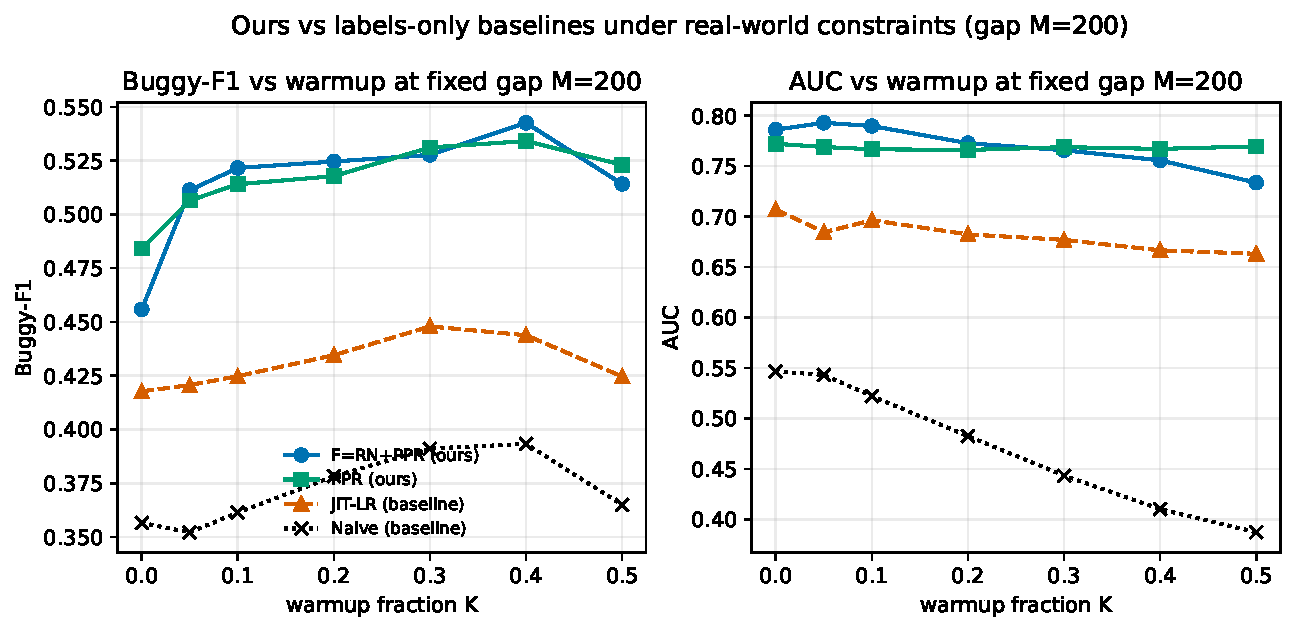
\includegraphics[width=\linewidth]{v4/param/fig_param_KM_compare}
		\caption{Real-world-constraint comparison at a fixed label gap $M{=}200$ over
		the warmup sweep: the deployed fusion $F$ and PPR (ours) versus the labels-only
		JIT-metrics LR and naive prior-rate baselines, on Buggy-F1 (left) and AUC
		(right). Our methods dominate throughout, with the largest margin at low
		warmup.}\label{fig:param-KM}
	\end{figure}

	\begin{figure}[t]\centering
		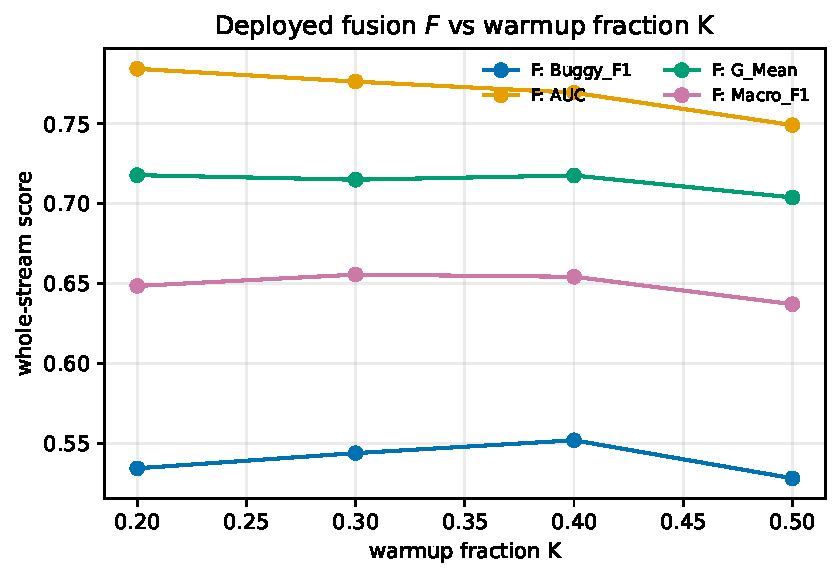
\includegraphics[width=.48\linewidth]{v4/param/fig_param_K_lines}\hfill
		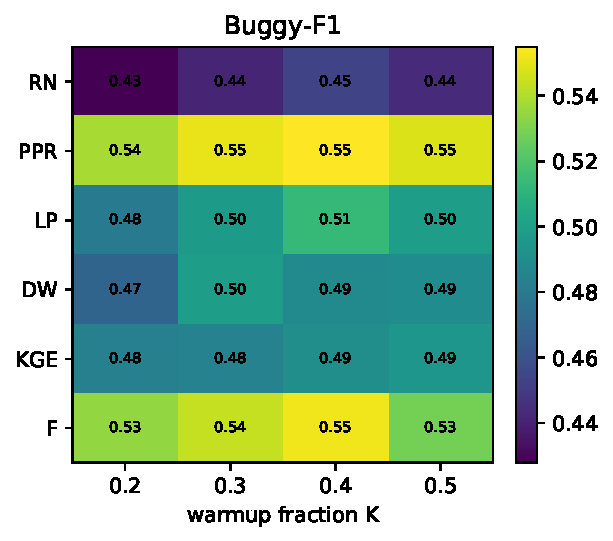
\includegraphics[width=.48\linewidth]{v4/param/fig_param_K_heat}
		\caption{Sensitivity to the warmup fraction $K$: deployed fusion metrics
		(left) and Buggy-F1 across methods (right). Near-flat with a mild peak at
		$K{\approx}0.4$.}\label{fig:param-K}
	\end{figure}

	\begin{figure}[t]\centering
		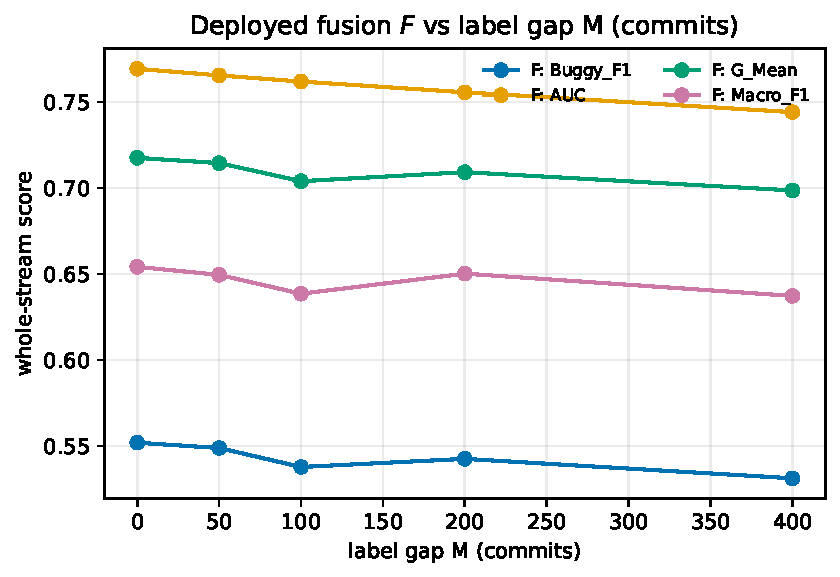
\includegraphics[width=.48\linewidth]{v4/param/fig_param_M_lines}\hfill
		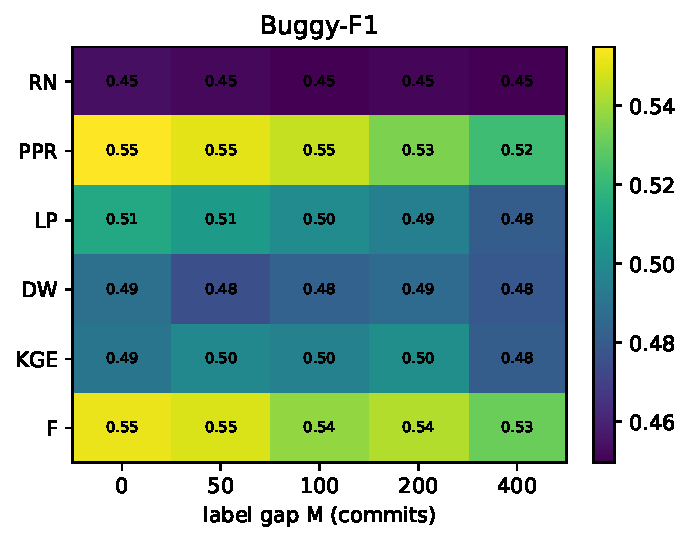
\includegraphics[width=.48\linewidth]{v4/param/fig_param_M_heat}
		\caption{Sensitivity to the label gap $M$: graceful degradation as recent
		labels are withheld, with no collapse --- the graph structure carries signal
		even when labels arrive late.}\label{fig:param-M}
	\end{figure}

	\begin{figure}[t]\centering
		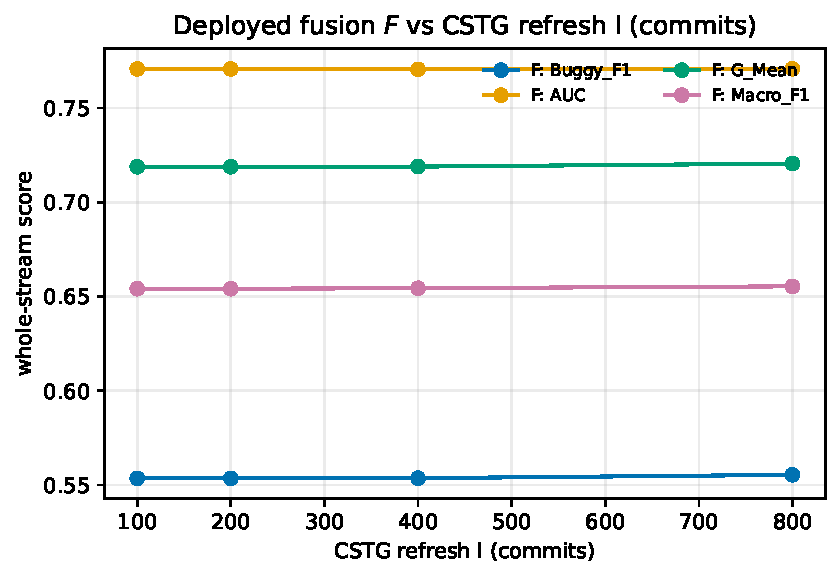
\includegraphics[width=.48\linewidth]{v4/param/fig_param_l_lines}\hfill
		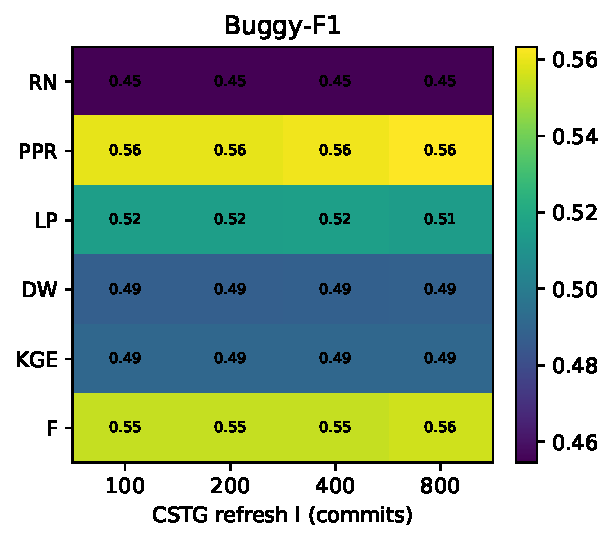
\includegraphics[width=.48\linewidth]{v4/param/fig_param_l_heat}
		\caption{Sensitivity to the online CSTG-hub refresh cadence $l$: the deployed
		fusion is essentially flat, so infrequent (cheap) refresh
		suffices.}\label{fig:param-l}
	\end{figure}

	\begin{figure}[t]\centering
		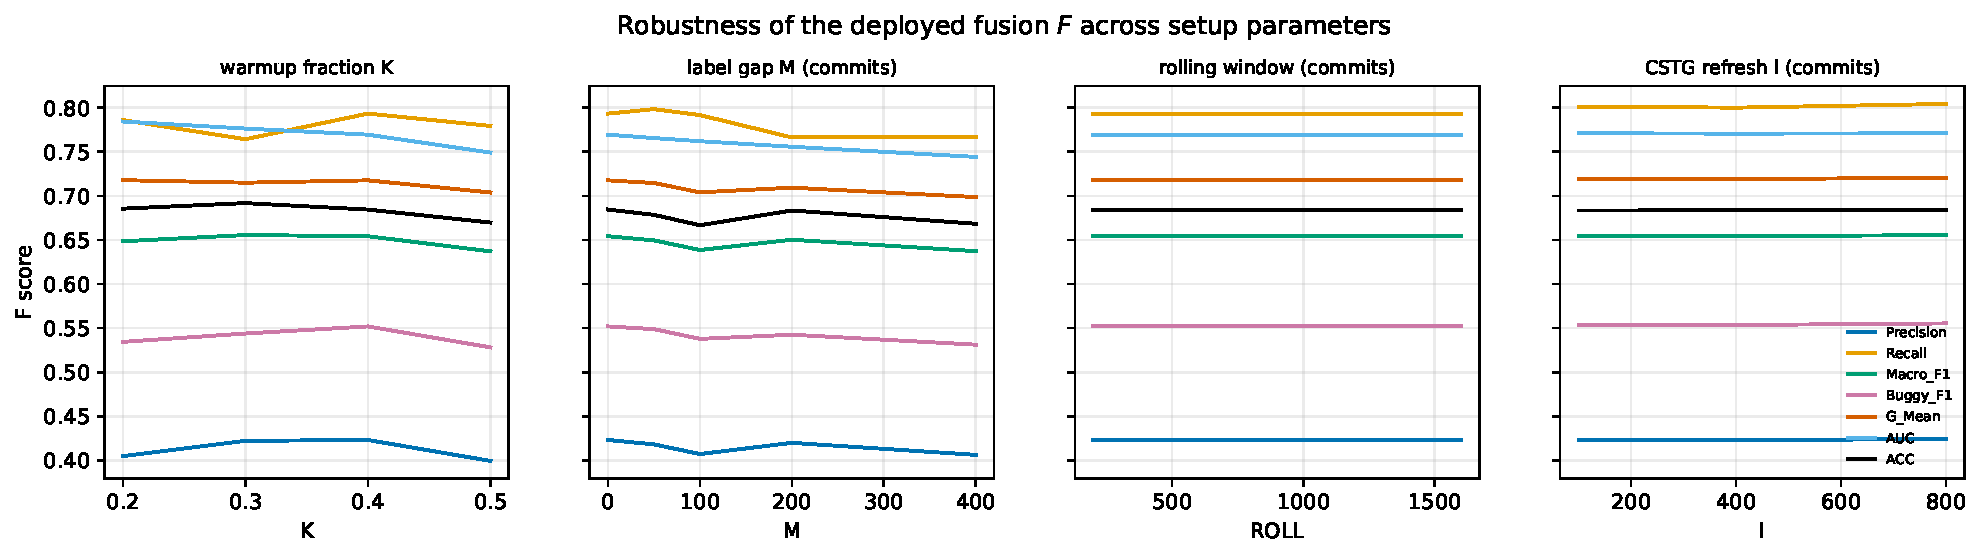
\includegraphics[width=\linewidth]{v4/param/fig_param_F_robustness}
		\caption{Robustness synthesis: the deployed fusion $F$'s seven headline
		metrics against each setup parameter. The model is stable throughout, so the
		headline conclusions do not depend on the setup.}\label{fig:param-robust}
	\end{figure}

\end{document}
